%---------------------------------------------------------------------------%
%-                                                                         -%
%-                           LaTeX Template                                -%
%-                                                                         -%
%---------------------------------------------------------------------------%
%- Copyright (C) Huangrui Mo <huangrui.mo@gmail.com> 
%- This is free software: you can redistribute it and/or modify it
%- under the terms of the GNU General Public License as published by
%- the Free Software Foundation, either version 3 of the License, or
%- (at your option) any later version.
%---------------------------------------------------------------------------%
%->> Document class declaration
%---------------------------------------------------------------------------%
\documentclass[twoside]{Style/ucasthesis}%
%- Multiple optional arguments:
%- [<oneside|twoside|print>]% oneside eprint, twoside eprint, or paper print
%- [fontset=<adobe|none|...>]% specify font set instead of automatic detection
%- [scheme=plain]% thesis writing of international students
%- [draftversion]% show draft version information
%- [standard options for ctex book class: draft|paper size|font size|...]%
%---------------------------------------------------------------------------%
%->> Document settings
%---------------------------------------------------------------------------%
\usepackage{caption}
\usepackage[super,list,table,math]{Style/artratex}
%- usage: \usepackage[option1,option2,...,optionN]{artratex}
%- Multiple optional arguments:
%- [bibtex|biber]% set bibliography processor and package
%- [<numbers|super|authoryear|alpha>]% set citation and reference style
%- <numbers>: textual: Jones [1]; parenthetical: [1]
%- <super>: textual: Jones superscript [1]; parenthetical: superscript [1]
%- <authoryear>: textual: Jones (1995); parenthetical: (Jones, 1995)
%- <alpha>: textual: not available; parenthetical: [Jon95]
%- [geometry]% reconfigure page layout via geometry package
%- [lscape]% provide landscape layout environment
%- [xhf]% disable header and footer via fancyhdr package
%- [color]% provide color support via xcolor package
%- [background]% enable page background
%- [tikz]% provide complex diagrams via tikz package
%- [table]% provide complex tables via ctable package
%- [list]% provide enhanced list environments for algorithm and coding
%- [math]% enable some extra math packages
%- [xlink]% disable link colors
\usepackage{Style/artracom}% user defined commands
%---------------------------------------------------------------------------%
%->> Document inclusion
%---------------------------------------------------------------------------%
%\includeonly{Tex/Chap_1,...,Tex/Chap_N}% selected files compilation
%---------------------------------------------------------------------------%
%->> Document content
%---------------------------------------------------------------------------%
%-
%-> Titlepage information
%-

%---------------------------------------------------------------------------%
%->> Titlepage information
%---------------------------------------------------------------------------%
%-
%-> 中文封面信息
%-
\confidential{}% 密级:涉密论文或延迟公开论文填写
\schoollogo[scale=0.095]{ucas_logo}% 校徽
\title{容器化环境中的横向移动检测方法}% 论文中文题目
\author{吴国璋}% 论文作者
\advisor{姜海洋~副研究员\\中国科学院计算技术研究所}% 指导教师:姓名 专业技术职务 工作单位
%\advisor{指导教师一\\指导教师二\\指导教师三}% 多行指导教师示例
\degree{硕士}% 学位:学士、硕士、博士
\degreetype{工学}% 学位类别:理学、工学、工程、医学等
\major{网络空间安全}% 一级/二级学科专业名称,领域名称需要与学籍信息一致
\institute{中国科学院计算技术研究所}% 院系名称
%\institute{中国科学院力学研究所\\流固耦合实验室}% 多行院系名称示例
\date{2024~年~6~月}% 毕业日期:夏季为6月、冬季为12月
%-
%-> 英文封面信息
%-
\TITLE{Lateral Movement Detection in Containerized Environments}% 论文英文题目
\AUTHOR{WU Guozhang}% 论文作者
\ADVISOR{Supervisor: Associate Professor JIANG Haiyang}% 指导教师
\DEGREE{Master}% 学位:Bachelor, Master, Doctor, Postdoctor。封面据英文学位名称自动切换,需确保拼写准确
\DEGREETYPE{Science in Engineering}% 学位类别:Philosophy, Natural Science, Engineering, Economics, Agriculture 等
\MAJOR{Cyber Security}% 二级学科专业名称
\INSTITUTE{Institute of Computing Technology, Chinese Academy of Sciences}% 院系名称
\DATE{June, 2024}% 毕业日期:夏季为June、冬季为December
%---------------------------------------------------------------------------%
%
\renewcommand\floatpagefraction{.9}
\renewcommand\topfraction{.9}
\renewcommand\bottomfraction{.9}
\renewcommand\textfraction{.1}
\begin{document}
%-
%-> Frontmatter: title page, abstract, content list, symbol list, preface
%-

\frontmatter% initialize the environment

%---------------------------------------------------------------------------%
%->> Frontmatter
%---------------------------------------------------------------------------%
%-
%-> 生成封面
%-

\maketitle% 生成中文封面
\MAKETITLE% 生成英文封面
%-
%-> 作者声明
%-
\makedeclaration% 生成声明页
%-
%-> 中文摘要
%-
\intobmk\chapter*{摘\quad 要}% 显示在书签但不显示在目录
\setcounter{page}{1}% 开始页码
\pagenumbering{Roman}% 页码符号

云计算技术的持续进步使得云原生容器平台成为企业数字化转型的核心。然而,随着容器化集群的广泛部署,许多集群受到各种攻击的困扰,安全性问题日益凸显。这些攻击可以分为若干个阶段,其中横向移动阶段的检测十分重要,在这一阶段,攻击者已进入集群中,开始收集集群内的信息,并寻找集群内的下一个攻击目标。尽管对于横向移动的检测在企业网络等环境中已有所研究,但针对容器化环境的检测方法仍然不足。

目前,容器化环境下的横向移动检测存在两方面的挑战:一是与已有研究的环境不同,容器化集群中的横向移动通常不包含用户身份验证信息,使得可用于检测的特征不明确;二是横向移动检测任务的横向移动检测任务的分类难度大,且样本不均衡,对高检测率和低误报率提出了高要求。

为了解决上述挑战,本文通过特征分析、特征重要度评估和特征嵌入方法对数据进行了增强,并提出了一种横向移动检测方法,提高了容器化环境中的检测性能。本文主要工作如下:

\begin{itemize}
    \item 针对容器化集群可用于检测的特征不明确的问题,本文从两个方面着手分析。在网络流量特征方面,本文进行了特征分析和特征重要度评估。通过数据集验证表明,通过特征分析,可发现横向移动流量中的``关键少数'',它们代表了攻击者在集群中部署恶意脚本并窃取机密信息的行为;通过特征重要度评估,可对重要性最低的特征进行筛除,节省 27\% 的模型训练时间。
    \item 在网络流量的时空特性方面,本文进行了拓扑分析和特征嵌入方法研究。通过拓扑分析,可以发现横向移动使网络拓扑发生改变,受感染的负载向 API 服务器非法通信的同时与外部网络保持联系;通过基于图神经网络的空间特征嵌入方法和基于循环神经网络的时间特征嵌入方法,可分别使模型的 AUC 分数提升 4 个和 3 个百分点。
    \item 针对横向移动检测任务的检测性能问题,本文提出了一种横向移动检测方法。该方法分两个阶段进行检测:首先,通过基于最值和拓扑的检测方法,本文从数据集中检出了关键的横向移动流量。在第二个阶段,提出了 LMDCE 模型,通过基于 Transformer 模型的编码器—解码器模块和两步预测机制,提升了检测的准确率,达到了 96.401\% 的 AUC 分数,超过了现有其他横向移动检测模型在容器化环境下的表现。
\end{itemize}

\keywords{容器化,横向移动,Transformer,自动编码器,入侵检测系统}% 中文关键词
%-
%-> 英文摘要
%-
\intobmk\chapter*{Abstract}% 显示在书签但不显示在目录

Continuous advances in cloud computing technology have made cloud-native containerized platforms the core of enterprise digital transformation. However, with the widespread deployment of containerized clusters, many clusters are plagued by various attacks, and security issues are becoming increasingly prominent. These attacks can be categorized into several phases, among which the detection of the lateral movement phase is very important. In this phase, the attacker has entered the cluster, starts to collect information within the cluster and looks for the next attack target within the cluster. Although lateral movement detection has been studied in environments such as enterprise networks, detection methods for containerized environments are still insufficient.

Currently, there are two challenges for lateral movement detection in containerized environments. First, unlike the environments that have been researched, lateral movements in containerized clusters usually do not contain user authentication information, making the features that can be used for detection unclear. Second, the difficulty of classifying lateral movement detection tasks with uneven samples puts a high demand on high detection rate and low false alarm rate.

To address the above challenges, this thesis enhances the data through feature analysis, feature importance evaluation and feature embedding methods, and proposes a lateral movement detection model to improve the detection performance in containerized environments. The main work of this thesis is as follows:

\begin{enumerate}
    \item Aiming at the problem that the features available for detection in containerized clusters are not clear, this thesis starts to analyze from two aspects. In terms of network flow features, this thesis performs feature analysis and feature importance assessment. Validation of the dataset shows that the feature analysis can identify the ``critical few'' in the lateral movement flows, which represent the attacker's behavior of deploying malicious scripts and stealing confidential information in the cluster; and the feature importance assessment can filter out the features with the lowest importance, which saves 27\% of the model training time. 

    \item In terms of the spatial and temporal characteristics of network flows, this thesis carries out research on topology analysis and feature embedding methods. Through topology analysis, it can be found that lateral movement changes the network topology, and the infected pod communicates illegally to the API server while keeping in touch with the external network; through the spatial feature embedding method based on graph neural network and the temporal feature embedding method based on recurrent neural network, the AUC scores of the model can be improved by 4 and 3 percentage points, respectively.

    \item Aiming at the detection performance problem of lateral movement detection task, this thesis proposes a lateral movement detection method. The method performs detection in two stages. First, through the detection method based on the most value and topology, this thesis detects critical lateral movement flows from the dataset. Second, this thesis proposes a model called LMDCE; the accuracy of detection is improved by a Transformer model-based encoder-decoder module and a two-phase prediction mechanism, achieving an AUC score of 96.401\%, which outperforms the performance of other existing lateral-movement detection models in a containerized environment.
\end{enumerate}
    %- the current style, comment all the lines in plain style definition.

\KEYWORDS{Containerization, Lateral Movement, Transformer, Autoencoder, Intrusion Detection System}% 英文关键词

\pagestyle{enfrontmatterstyle}%
\cleardoublepage\pagestyle{frontmatterstyle}%

%---------------------------------------------------------------------------%
% title page, abstract

{% content list region
\linespread{1.2}% local line space
\intobmk*{\cleardoublepage}{\contentsname}% add link to bookmark
\tableofcontents% content catalog

\intobmk*{\cleardoublepage}{图表目录}
\thispagestyle{noheaderstyle}

{
\renewcommand*{\addvspace}[1]{}
\let\oldnumberline\numberline%
\renewcommand{\numberline}{\figurename~\oldnumberline}%
\listoffigures%
\renewcommand{\numberline}{\appfigname~\oldnumberline}%
\let\cleardoublepage\relax
\let\clearpage\relax
\vspace{-30pt}
\listofappfigs
}
{
\let\cleardoublepage\relax
\let\clearpage\relax
\renewcommand*{\addvspace}[1]{}
\let\oldnumberline\numberline%
\renewcommand{\numberline}{\tablename~\oldnumberline}%
\listoftables%

\renewcommand{\numberline}{\apptabname~\oldnumberline}%
\let\cleardoublepage\relax
\let\clearpage\relax
\vspace{-30pt}
\listofapptabs
}

\thispagestyle{figureheader}
}
% \intobmk\chapter*{符号列表}% 显示在书签但不显示在目录

\section*{字符}
\nomenclatureitem[\textbf{Unit}]{\textbf{Symbol}}{\textbf{Description}}
\nomenclatureitem[$\Unit{m^{2} \cdot s^{-2} \cdot K^{-1}}$]{$R$}{the gas constant}
\nomenclatureitem[$\Unit{m^{2} \cdot s^{-2} \cdot K^{-1}}$]{$C_v$}{specific heat capacity at constant volume}
\nomenclatureitem[$\Unit{m^{2} \cdot s^{-2} \cdot K^{-1}}$]{$C_p$}{specific heat capacity at constant pressure}
\nomenclatureitem[$\Unit{m^{2} \cdot s^{-2}}$]{$E$}{specific total energy}
\nomenclatureitem[$\Unit{m^{2} \cdot s^{-2}}$]{$e$}{specific internal energy}
\nomenclatureitem[$\Unit{m^{2} \cdot s^{-2}}$]{$h_T$}{specific total enthalpy}
\nomenclatureitem[$\Unit{m^{2} \cdot s^{-2}}$]{$h$}{specific enthalpy}
\nomenclatureitem[$\Unit{kg \cdot m \cdot s^{-3} \cdot K^{-1}}$]{$k$}{thermal conductivity}
\nomenclatureitem[$\Unit{kg \cdot m^{-1} \cdot s^{-2}}$]{$S_{ij}$}{deviatoric stress tensor}
\nomenclatureitem[$\Unit{kg \cdot m^{-1} \cdot s^{-2}}$]{$\tau_{ij}$}{viscous stress tensor}
\nomenclatureitem[$\Unit{1}$]{$\delta_{ij}$}{Kronecker tensor}
\nomenclatureitem[$\Unit{1}$]{$I_{ij}$}{identity tensor}

\section*{算子}
\nomenclatureitem{\textbf{Symbol}}{\textbf{Description}}
\nomenclatureitem{$\Delta$}{difference}
\nomenclatureitem{$\nabla$}{gradient operator}
\nomenclatureitem{$\delta^{\pm}$}{upwind-biased interpolation scheme}

\section*{缩写}
\nomenclatureitem{CFD}{Computational Fluid Dynamics}
\nomenclatureitem{CFL}{Courant-Friedrichs-Lewy}
\nomenclatureitem{EOS}{Equation of State}
\nomenclatureitem{JWL}{Jones-Wilkins-Lee}
\nomenclatureitem{WENO}{Weighted Essentially Non-oscillatory}
\nomenclatureitem{ZND}{Zel'dovich-von Neumann-Doering}

% symbol list, preface content
%-
%-> Mainmatter
%-
\mainmatter% initialize the environment

%---------------------------------------------------------------------------%
%->> Main content
%---------------------------------------------------------------------------%
\renewcommand{\thefigure}{\thechapter-\arabic{figure}}
\renewcommand{\thetable}{\thechapter-\arabic{table}}
\renewcommand{\theequation}{\thechapter-\arabic{equation}}
% \chapter{绪论}\label{chap:introduction}{

\section{背景}

2022年修订的《中国科学院大学研究生学位论文撰写规范和指导意见》(以下简称《指导意见》)从2023年冬季批次开始实施。为方便各位同学使用,特提供此模板。

您在使用此模板进行学位论文撰写时,只需根据《指导意见》在相应章节填写具体内容即可。

本模板在第2章提供了本模板的使用说明,在第3章中提供了《指导意见》中关于内容和格式的部分要求,请仔细阅读。


\section{系统要求}\label{sec:system}
\begin{table}
    \bicaption{\enspace 支持的LaTeX编译系统和编辑器}{\enspace Supported LaTeX compiler and editor}% caption
    \footnotesize% fontsize
    \setlength{\tabcolsep}{4pt}% column separation
    \renewcommand{\arraystretch}{1.5}% row space 
    \centering
    \begin{tabular}{lcc}
        \hline
        %\multicolumn{num_of_cols_to_merge}{alignment}{contents} \\
        %\cline{i-j}% partial hline from column i to column j
        操作系统 & LaTeX编译系统 & LaTeX文本编辑器\\
        \hline
        Windows & \href{https://www.tug.org/texlive/acquire-netinstall.html}{TexLive Full} 或 \href{https://miktex.org/download}{MiKTex} & \href{http://www.xm1math.net/texmaker/}{Texmaker}\\
        Linux & \href{https://www.tug.org/texlive/acquire-netinstall.html}{TexLive Full} & \href{http://www.xm1math.net/texmaker/}{Texmaker} 或 Vim\\
        MacOS & \href{https://www.tug.org/mactex/}{MacTex Full} & \href{http://www.xm1math.net/texmaker/}{Texmaker} 或 Texshop\\
        Overleaf & XeLaTeX+TexLive2021 & Overleaf \\
        \hline
    \end{tabular}
    \label{tab:compiler}
\end{table}
\href{https://github.com/mohuangrui/ucasthesis}{\texttt{ucasthesis}} 宏包可以在目前主流的 \href{https://en.wikibooks.org/wiki/LaTeX/Introduction}{LaTeX} 编译系统中使用,如TexLive和MiKTeX。因CTex套装已停止维护,\textbf{不再建议使用} (请勿混淆CTex套装与ctex宏包。CTex套装是集成了许多LaTeX组件的LaTeX编译系统。 \href{https://ctan.org/pkg/ctex?lang=en}{ctex} 宏包如同ucasthesis,是LaTeX命令集,其维护状态活跃,并被主流的LaTeX编译系统默认集成,是几乎所有LaTeX中文文档的核心架构)。推荐的 \href{https://en.wikibooks.org/wiki/LaTeX/Installation}{LaTeX编译系统} 和 \href{https://en.wikibooks.org/wiki/LaTeX/Installation}{LaTeX文本编辑器} 为LaTeX编译系统见表~\ref{tab:compiler}。请从各软件官网下载安装程序,勿使用不明程序源。LaTeX编译系统和LaTeX编辑器分别安装成功后,即完成了LaTeX的系统配置,无需其他手动干预和配置。若系统原带有旧版的LaTeX编译系统并想安装新版,请\textbf{先卸载干净旧版再安装新版}。

使用overleaf在线编辑是一种简单有效的方法,对于绝大多数初学者来说,我们推荐使用这种无需进行系统配置的方式。在操作时,只需将压缩包上传至网站即可,无需在本地配置环境,同时支持多人,多地撰写论文。

本模板兼容操作系统:Windows、Linux、MacOS、Overleaf在线编辑器,支持多种LaTeX编译引擎(pdfLaTeX、xeLaTeX、luaLaTeX)。}

% \chapter{LaTeX使用说明}\label{chap:guide}

{
为方便使用及更好地展示LaTeX排版的优秀特性,ucasthesis的框架和文件体系进行了细致地处理,尽可能地对各个功能和板块进行了模块化和封装。

\section{初步设置}

\begin{enumerate}
    \item 使用overleaf:打开并注册\href{https://cn.overleaf.com/}{overleaf}。
    \item 将整个文件夹上传至overleaf项目。
    \item 右键菜单,设置编译器为XeLaTeX,选择TexLive 2021
    \item 点击编译,即可预览PDF文件
\end{enumerate}
编译完成即可获得本PDF说明文档。

\section{文档目录简介}

\subsection{Thesis.tex}

Thesis.tex为主文档,其设计和规划了论文的整体框架,通过对其的阅读可以了解整个论文框架的搭建。

\subsection{编译脚本}

为方便本地编译,提供bat脚本和.sh脚本分别用于windows环境和unix环境。

\begin{itemize}
    \item Windows:双击Dos脚本artratex.bat可得全编译后的PDF文档,其存在是为了帮助不了解LaTeX编译过程的初学者跨过编译这第一道坎,请勿通过邮件传播和接收此脚本,以防范Dos脚本的潜在风险。
    \item Linux或MacOS:在terminal中运行
        \begin{itemize}
            \item \verb|./artratex.sh xa|:获得全编译后的PDF文档
            \item \verb|./artratex.sh x|:快速编译,不会生成文献引用
        \end{itemize}
\end{itemize}

全编译指运行 \verb|xeLaTeX+bibtex+xeLaTeX+xeLaTeX| 以正确生成所有的引用链接,如目录、参考文献及引用等。在写作过程中若无添加新的引用,则可用快速编译,即只运行一遍LaTeX编译引擎以减少编译时间。

\subsection{Tmp文件夹}

运行编译脚本后,编译所生成的文档皆存于Tmp文件夹内,包括编译得到的PDF文档,其存在是为了保持工作空间的整洁。

\subsection{Style文件夹}

包含ucasthesis文档类的定义文件和配置文件,通过对它们的修改可以实现特定的模版设定。

\begin{enumerate}
    \item ucasthesis.cls:文档类定义文件,论文的最核心的格式即通过它来定义的。
    \item ucasthesis.cfg:文档类配置文件,设定如目录显示为“目~录”而非“目录”。
    \item artratex.sty: 常用宏包及文档设定,如参考文献样式、文献引用样式、页眉页脚设定等。这些功能具有开关选项,常只需在Thesis.tex中进行启用即可,一般无需修改artratex.sty本身。
    \item artracom.sty:自定义命令以及添加宏包的推荐放置位置。
\end{enumerate}

\subsection{Tex文件夹}

文件夹内为论文的所有实体内容,正常情况下,这也是使用ucasthesis撰写学位论文时,主要关注和修改的一个位置,注:所有文件都必须采用UTF-8编码,否则编译后将出现乱码文本,详细分类介绍如下:

\begin{itemize}
    \item Frontinfo.tex:为论文中英文封面信息。论文封面会根据英文学位名称如Master,Doctor自动切换为相应的格式。
    \item Frontmatter.tex:为论文前言内容如中英文摘要等。
    \item Mainmatter.tex:索引需要出现的Chapter。开始写论文时,可以只索引当前章节,以快速编译查看,当论文完成后,再对所有章节进行索引即可。
    \item Chap{\_}xxx.tex:为论文主体的各章,可根据需要添加和撰写。添加新章时,可拷贝一个已有的章文件再重命名,以继承文档的 UTF8 编码。
    \item Appendix.tex:为附录内容。
    \item Backmatter.tex:为发表文章信息和致谢部分等。
\end{itemize}

\subsection{Img文件夹}

用于放置论文中所需要的图类文件,支持格式有:.jpg, .png, .pdf。其中,\verb|ucas_logo.pdf|为国科大校徽。

\subsection{Biblio文件夹}

 ref.bib用于放置论文中所需要参考文献信息。

\section{功能介绍}

\subsection{数学公式}

比如Navier-Stokes方程(方程~\eqref{eq:ns}):
\begin{equation} \label{eq:ns}
    %\adddotsbeforeeqnnum%
    \begin{cases}
        \frac{\partial \rho}{\partial t} + \nabla\cdot(\rho\Vector{V}) = 0 \ \mathrm{times\ math\ test: 1,2,3,4,5}, 1,2,3,4,5\\
        \frac{\partial (\rho\Vector{V})}{\partial t} + \nabla\cdot(\rho\Vector{V}\Vector{V}) = \nabla\cdot\Tensor{\sigma} \ \text{times text test: 1,2,3,4,5}\\
        \frac{\partial (\rho E)}{\partial t} + \nabla\cdot(\rho E\Vector{V}) = \nabla\cdot(k\nabla T) + \nabla\cdot(\Tensor{\sigma}\cdot\Vector{V})
    \end{cases}
\end{equation}
\begin{equation}
    %\adddotsbeforeeqnnum%
    \frac{\partial }{\partial t}\int\limits_{\Omega} u \, \mathrm{d}\Omega + \int\limits_{S} \unitVector{n}\cdot(u\Vector{V}) \, \mathrm{d}S = \dot{\phi}
\end{equation}
\[
    \begin{split}
        \mathcal{L} \{f\}(s) &= \int _{0^{-}}^{\infty} f(t) e^{-st} \, \mathrm{d}t, \ 
        \mathscr{L} \{f\}(s) = \int _{0^{-}}^{\infty} f(t) e^{-st} \, \mathrm{d}t\\
        \mathcal{F} {\bigl (} f(x+x_{0}) {\bigr )} &= \mathcal{F} {\bigl (} f(x) {\bigr )} e^{2\pi i\xi x_{0}}, \ 
        \mathscr{F} {\bigl (} f(x+x_{0}) {\bigr )} = \mathscr{F} {\bigl (} f(x) {\bigr )} e^{2\pi i\xi x_{0}}
    \end{split}
\]

数学公式常用命令请见 \href{https://en.wikibooks.org/wiki/LaTeX/Mathematics}{WiKibook Mathematics}。artracom.sty中对一些常用数据类型如矢量矩阵等进行了封装,这样的好处是如有一天需要修改矢量的显示形式,只需单独修改artracom.sty中的矢量定义即可实现全文档的修改。

\subsection{数学环境}

\begin{axiom}
   这是一个公理。 
\end{axiom}
\begin{theorem}
   这是一个定理。 
\end{theorem}
\begin{lemma}
   这是一个引理。 
\end{lemma}
\begin{corollary}
   这是一个推论。 
\end{corollary}
\begin{assertion}
   这是一个断言。 
\end{assertion}
\begin{proposition}
   这是一个命题。 
\end{proposition}
\begin{definition}
    这是一个定义。
\end{definition}
\begin{example}
    这是一个例子。
\end{example}
\begin{remark}
    这是一个注。
\end{remark}

\subsection{图}

论文中图片的插入通常分为单图和多图,下面分别加以介绍:

单图插入:假设插入名为\verb|c06h06|(后缀可以为.jpg、.png和.pdf,下同)的图片,其效果如图~\ref{fig:c06h06}。
\begin{figure}[!htbp]
    \centering
    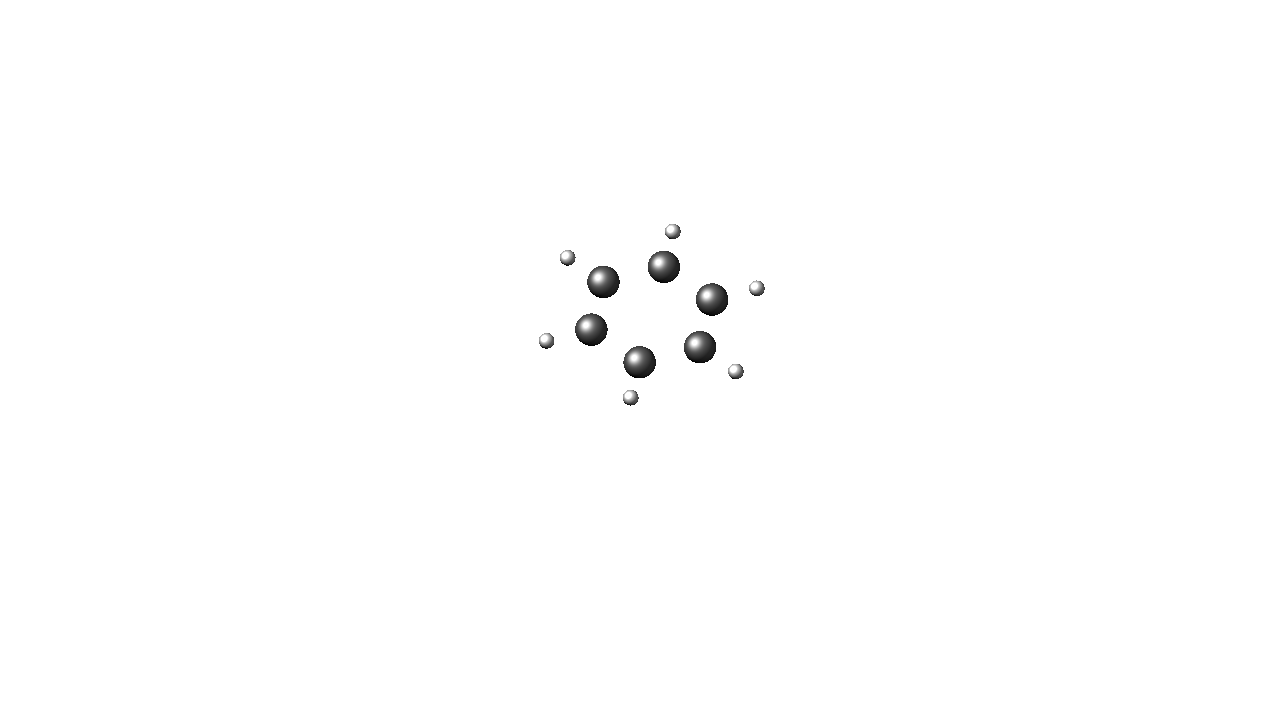
\includegraphics[width=0.40\textwidth]{c06h06}
    \bicaption{\enspace 样图}{\enspace Sample Figure}
    \fignote{对图片的注释}
    \label{fig:c06h06}

\end{figure}

如果插图的空白区域过大,以图片\verb|c06h06|为例,自动裁剪如图~\ref{fig:c06h06_trim}。
\begin{figure}[!htbp]
    \centering
    %trim option's parameter order: left bottom right top
    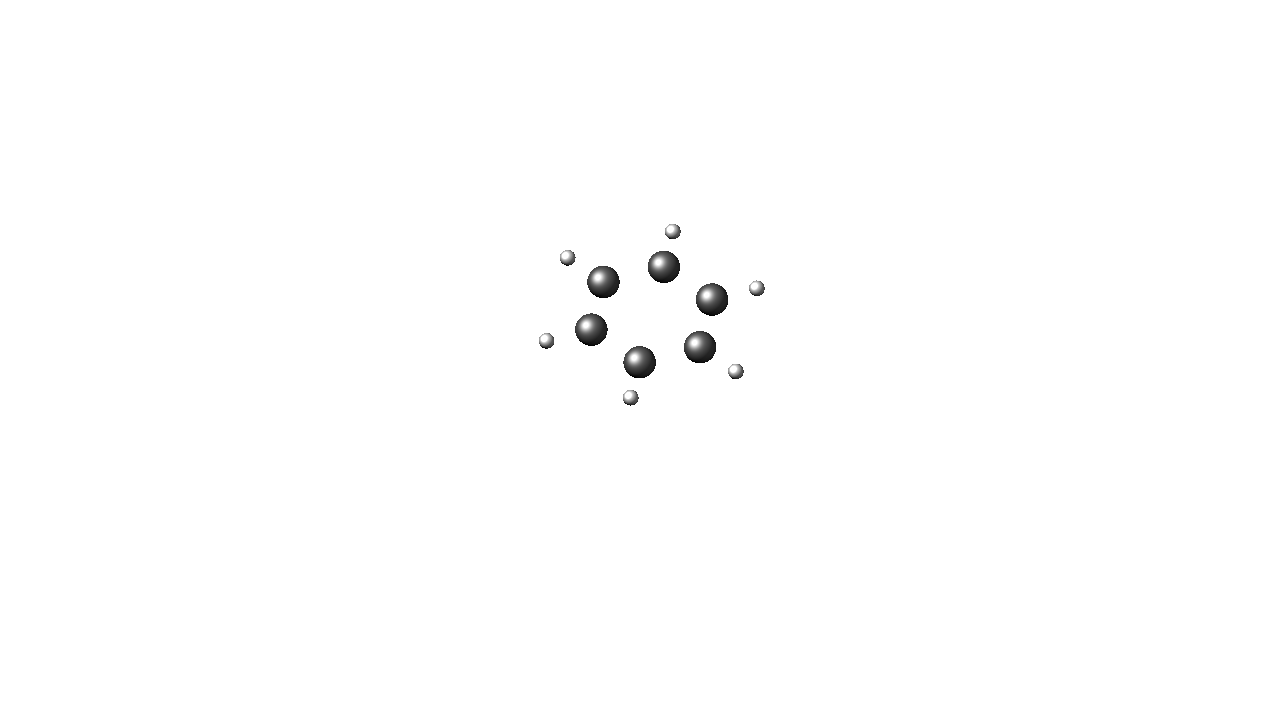
\includegraphics[trim = 60mm 80mm 60mm 60mm, clip, width=0.40\textwidth]{c06h06}
    \bicaption{\enspace 自动裁切测试}{\enspace Auto-Crop Test}
    \label{fig:c06h06_trim}
\end{figure}

多图的插入如图~\ref{fig:oaspl},多图不应在子图中给文本子标题,只要给序号,并在主标题中进行引用说明。
\begin{figure}[!htbp]
    \centering
    \begin{subfigure}[b]{0.35\textwidth}
      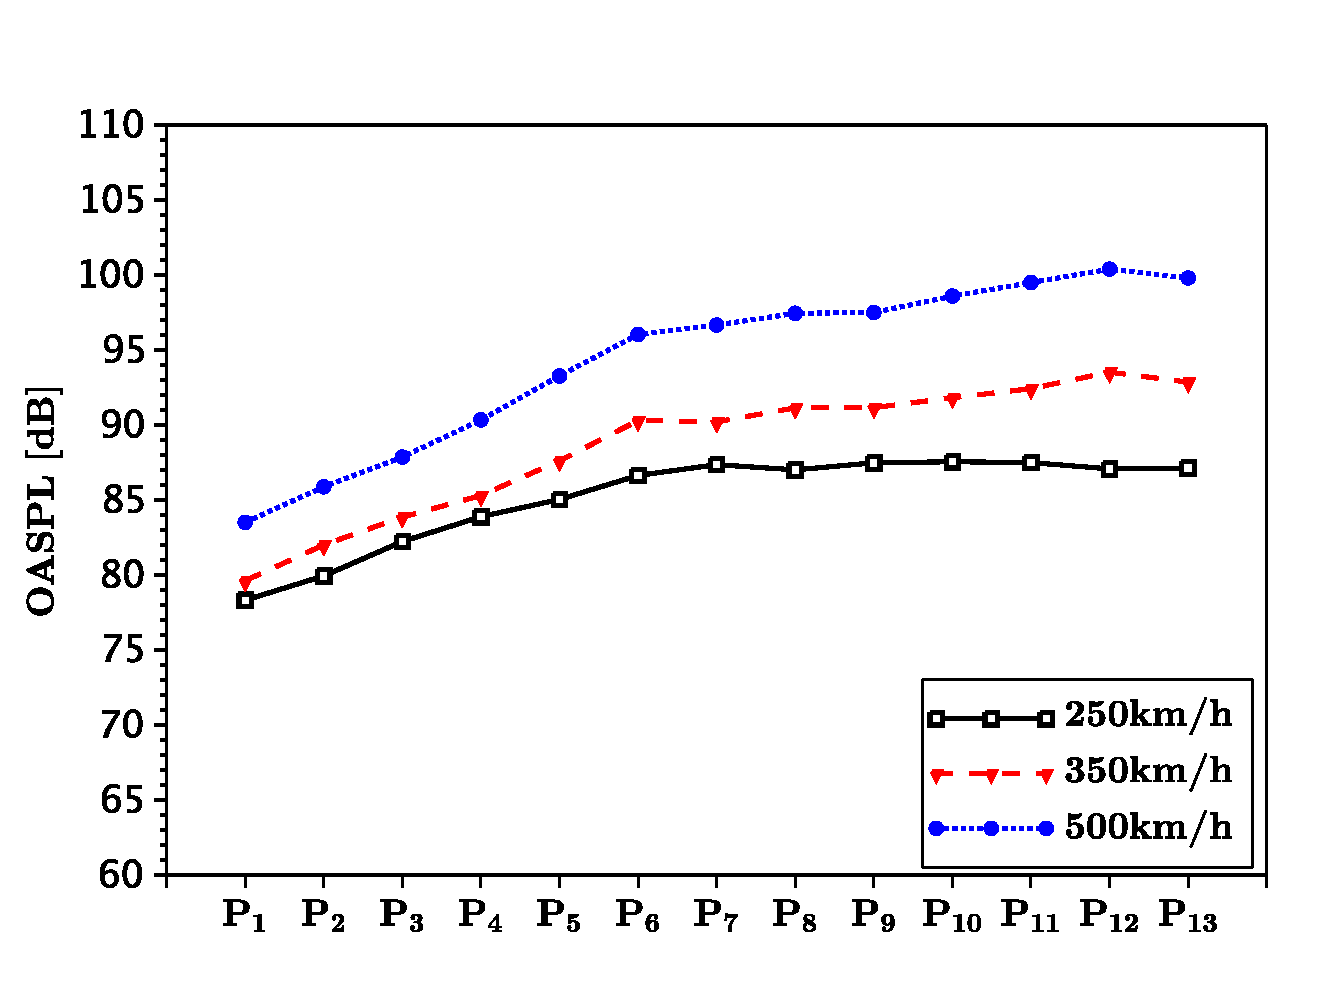
\includegraphics[width=\textwidth]{oaspl_a}
      \caption{}
      \label{fig:oaspl_a}
    \end{subfigure}%
    ~% add desired spacing
    \begin{subfigure}[b]{0.35\textwidth}
      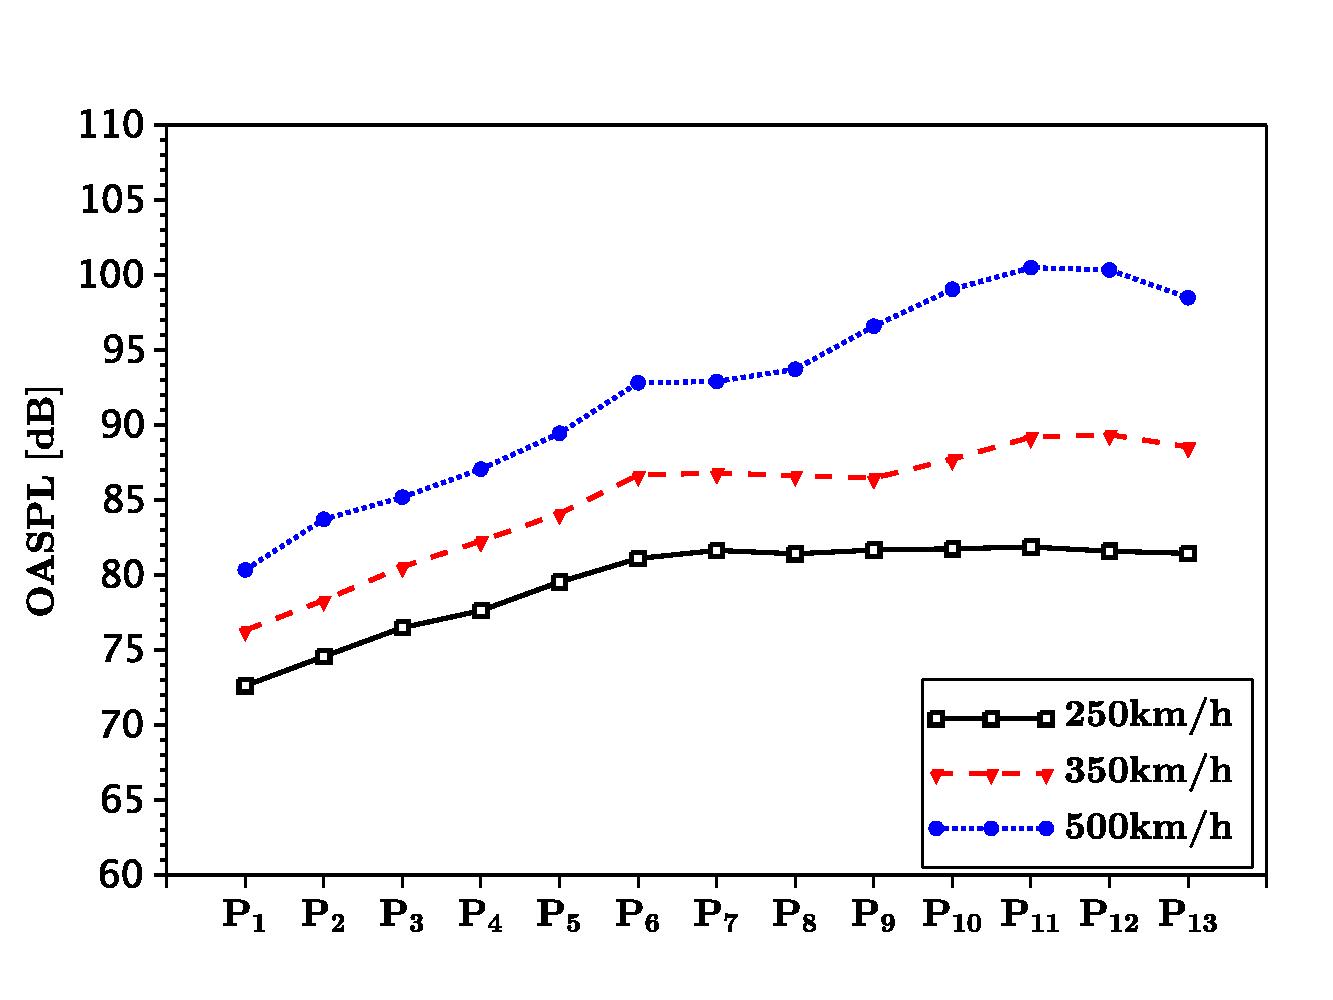
\includegraphics[width=\textwidth]{oaspl_b}
      \caption{}
      \label{fig:oaspl_b}
    \end{subfigure}
    \\% line break
    \begin{subfigure}[b]{0.35\textwidth}
      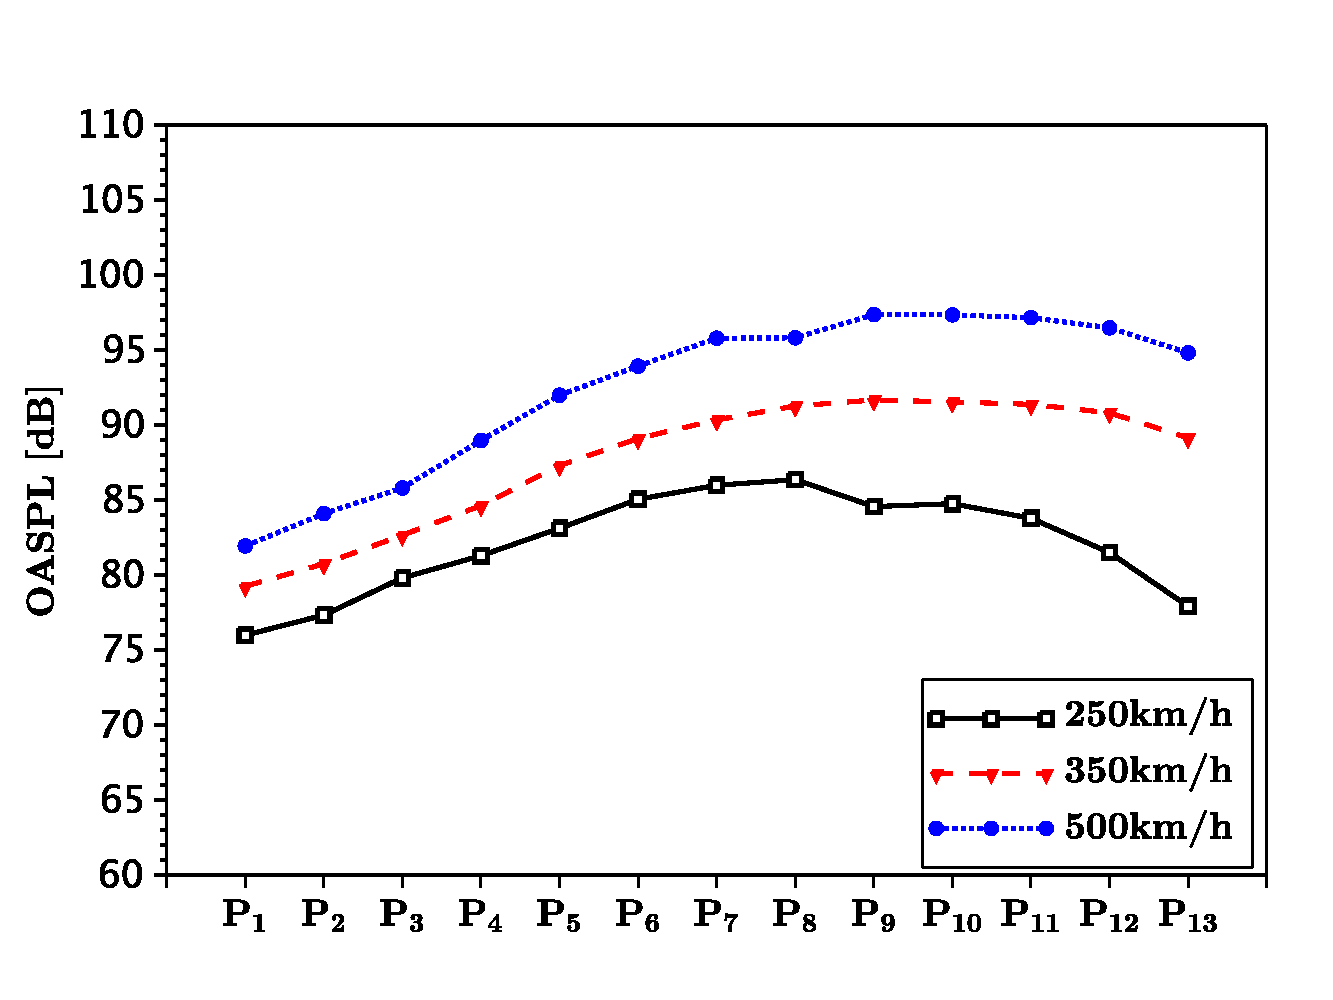
\includegraphics[width=\textwidth]{oaspl_c}
      \caption{}
      \label{fig:oaspl_c}
    \end{subfigure}%
    ~% add desired spacing
    \begin{subfigure}[b]{0.35\textwidth}
      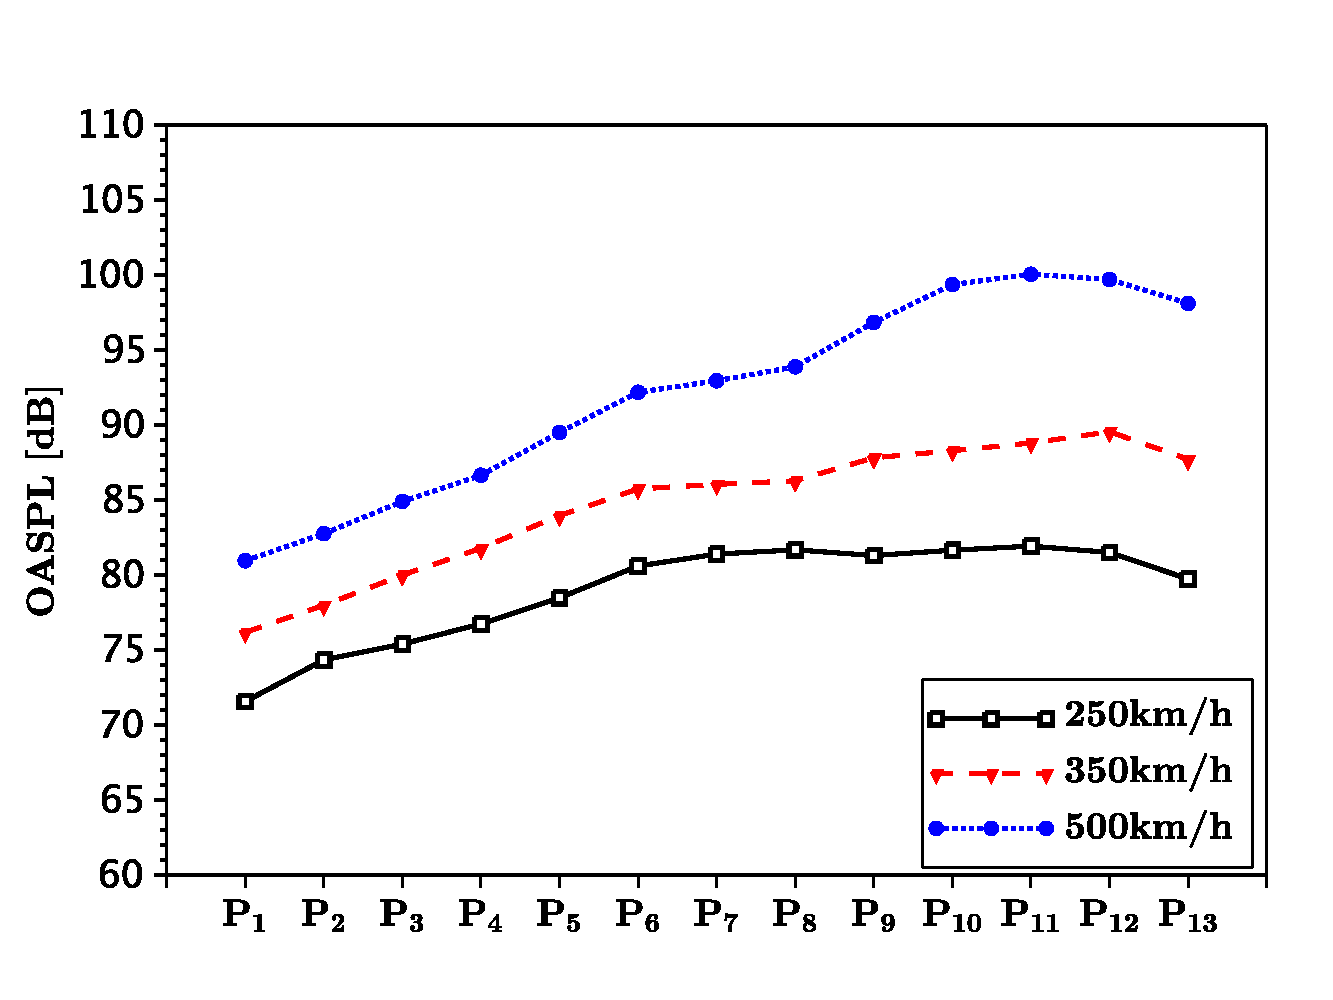
\includegraphics[width=\textwidth]{oaspl_d}
      \caption{}
      \label{fig:oaspl_d}
    \end{subfigure}
    \bicaption{\enspace 多子图测试}{\enspace A test for multi-subfig}
    \label{fig:oaspl}
\end{figure}

\subsection{表}

请见表~\ref{tab:sample}。
\begin{table}[!htbp]
    \bicaption{\enspace 这是一个样表}{\enspace This is a sample table}
    \label{tab:sample}
    \centering
    \footnotesize% fontsize
    \setlength{\tabcolsep}{4pt}% column separation
    \renewcommand{\arraystretch}{1.2}%row space 
    \begin{tabular}{lcccccccc}
        \hline
        行号 & \multicolumn{8}{c}{跨多列的标题}\\
        %\cline{2-9}% partial hline from column i to column j
        \hline
        Row 1 & $1$ & $2$ & $3$ & $4$ & $5$ & $6$ & $7$ & $8$\\
        Row 2 & $1$ & $2$ & $3$ & $4$ & $5$ & $6$ & $7$ & $8$\\
        Row 3 & $1$ & $2$ & $3$ & $4$ & $5$ & $6$ & $7$ & $8$\\
        Row 4 & $1$ & $2$ & $3$ & $4$ & $5$ & $6$ & $7$ & $8$\\
        \hline
    \end{tabular}
\end{table}

制图制表的更多范例,请见 \href{https://github.com/mohuangrui/ucasthesis/wiki}{ucasthesis 知识小站} 和 \href{https://en.wikibooks.org/wiki/LaTeX/Tables}{WiKibook Tables}。

\subsection{参考文献引用}

参考文献引用过程以实例进行介绍,假设需要引用名为"Document Preparation System"的文献,步骤如下:

1)将Bib格式的参考文献信息添加到ref.bib文件中(此文件位于Biblio文件夹下),如直接粘贴自网站,请注意修改其格式。

2)索引第一行 \verb|@article{lamport1986document,|中 \verb|lamport1986document| 即为此文献的label (中文文献也必须使用英文label,一般遵照:姓氏拼音+年份+标题第一字拼音的格式),想要在论文中索引此文献,\verb|\citep{lamport1986document}|。如此处所示 \citep{lamport1986document}。

多文献索引用英文逗号隔开, 如此处所示 \citep{lamport1986document, chu2004tushu, chen2005zhulu}。

更多例子如:

Walls等\citep{walls2013drought}根据Betts\citep{betts2005aging} 的研究,首次提出......理论。其中关于......的研究\citep{walls2013drought, betts2005aging},是当前中国得到迅速发展的研究领域 \citep{chen1980zhongguo, bravo1990comparative}。

不同文献样式和引用样式,如著者-出版年制(authoryear)、顺序编码制(numbers)、上标顺序编码制(super)可在Thesis.tex中对artratex.sty调用实现,详见 \href{https://github.com/mohuangrui/ucasthesis/wiki}{ucasthesis 知识小站之文献样式}。

%若在上标顺序编码制(super)模式下,希望在特定位置将上标改为嵌入式标,可使用 \citetns{niu2013zonghe,stamerjohanns2009mathml} 和 \citepns{niu2013zonghe,stamerjohanns2009mathml}。

参考文献索引的更多知识,请见 \href{https://en.wikibooks.org/wiki/LaTeX/Bibliography_Management}{WiKibook Bibliography}。\nocite{*}% 使文献列表显示所有参考文献(包括未引用文献)

\section{常见使用问题}\label{sec:qa}

设置文档样式: 在artratex.sty中搜索关键字定位相应命令,然后修改
\begin{enumerate}
    \item 正文行距:启用和设置 \verb|\linespread{1.25}|,默认1.25倍行距。
    \item 参考文献行距:修改 \verb|\setlength{\bibsep}{0.0ex}|
    \item 目录显示级数:修改 \verb|\setcounter{tocdepth}{2}|
    \item 文档超链接的颜色及其显示:修改 \verb|\hypersetup|
\end{enumerate}

文档内字体切换方法:
    \begin{itemize}
        \item 宋体:国科大论文模板ucasthesis 或 \textrm{国科大论文模板ucasthesis}
        \item 粗宋体:{\bfseries 国科大论文模板ucasthesis} 或 \textbf{国科大论文模板ucasthesis}
        \item 黑体:{\sffamily 国科大论文模板ucasthesis} 或 \textsf{国科大论文模板ucasthesis}
        \item 粗黑体:{\bfseries\sffamily 国科大论文模板ucasthesis} 或 \textsf{\bfseries 国科大论文模板ucasthesis}
        \item 仿宋:{\ttfamily 国科大论文模板ucasthesis} 或 \texttt{国科大论文模板ucasthesis}
        \item 粗仿宋:{\bfseries\ttfamily 国科大论文模板ucasthesis} 或 \texttt{\bfseries 国科大论文模板ucasthesis}
        \item 楷体:{\itshape 国科大论文模板ucasthesis} 或 \textit{国科大论文模板ucasthesis}
        \item 粗楷体:{\bfseries\itshape 国科大论文模板ucasthesis} 或 \textit{\bfseries 国科大论文模板ucasthesis}
    \end{itemize}
    
对附录的引用,如对附录\ref{chap:app1}的引用。
对附录中图表的引用,如,对附表\ref{apptab:1}的引用。
\let\cleardoublepage\relax
}

% \chapter{中国科学院大学
研究生学位论文撰写规范指导意见(节选)}{
{
\let\cleardoublepage\relax
}
学位论文是研究生在掌握已有的科学知识的基础上,运用科学思维和一定的科学方法、技术与工具,面向特定的科学领域所存在的科学问题,开展创新性研究而产生的科学研究成果。

学位论文是研究生科研工作成果的集中体现,是评判学位申请者学术水平、授予其学位的主要依据,是科研领域重要的文献资料。撰写学位论文是对研究生科学研究能力的基本训练,是研究生学业与研究成效的基本检验,也是科研与创新能力的重要体现。

为提高研究生学位论文的撰写质量,促进学位论文在内容和格式上的规范化,参照《学位论文编写规则》(GB/T 7713.1—2006)、《信息与文献 参考文献著录规则》(GB/T 7714—2015)和《学术出版规范 期刊学术不端行为界定》(CY/T 174—2019)等国家有关标准,特制定本指导意见(2021年修订)。各学科群学位评定分委员会(以下简称各学科群分会)可结合本学科领域的特点,参考本指导意见,制订符合本学科领域特点与要求的学位论文撰写具体要求。

本指导意见从2023年冬季批次开始实施。

\section{组成及要求}
学位论文一般由以下几个部分组成:封面、原创性声明及授权使用声明、摘要、目录、符号说明(若有)、正文、参考文献、附录(若有)、致谢、作者简历及攻读学位期间发表的学术论文与其他相关学术成果等。
\subsection{封面}
一律采用中国科学院大学规定的统一中英文封面,封面包含内容如下:

\begin{enumerate}
    \item 密级,涉密或延迟公开论文必须在论文封面标注密级,同时注明保密年限。公开论文不标注密级,可删除此行。
    \item 论文题目,应简明扼要地概括和反映整个论文的核心内容,一般不宜超过25个汉字(符),英文题目一般不应超过150个字母,必要时可加副标题。题目中应尽量避免使用缩略词、首字母缩写词、字符、代号和公式等。
    \item 作者姓名,根据《中国人名汉语拼音字母拼写规则》(GB/T 28039—2011),英文封面中的姓和名分写,姓在前,名在后,姓名之间用空格分开。姓和名需写全拼,姓全大写,名首字母大写。外国留学生姓名书写顺序以护照格式为准,字母全部大写。
    \item 指导教师,需同时填写导师姓名、专业技术职务和工作单位。如果有多位导师(均需经培养单位批准,并在学籍系统备案),第一导师在前,第二导师等依次在后。学位论文在指导小组的指导下完成的,应注明指导小组成员相应信息。
    \item 学位类别,包括学科门类(学术型)或专业学位类别以及学位级别。学科门类如理学、医学等,专业学位类别如应用统计、工商管理等。学位级别包括硕士、博士。
    \item 学科专业,填写攻读学位的一级学科/二级学科或专业学位类别/领域全称,须与学籍信息一致,不可用简写。
    \item 培养单位,填写就读研究所或学院、系全称,如中国科学院××研究所、中国科学院大学××学院。
    \item 时间,填写论文提交学位授予单位的年月,使用阿拉伯数字标注。一般夏季申请学位的论文标注6月,冬季申请学位的论文标注12月。例如:2023年6月,2023年12月。
\end{enumerate}

\subsection{原创性声明及授权使用声明}
本部分内容提供统一的模版,提交时作者和导师须亲笔签名。如遇导师无法签字时,培养单位应做出适当处理。
\subsection{摘要和关键词}
论文摘要包括中文摘要和英文摘要(Abstract)两部分。论文摘要应概括地反映出本论文的主要内容,说明本论文的主要研究目的、内容、方法、结论。要突出本论文的创造性成果或新见解,不宜使用公式、图表、表格或其他插图材料,不标注引用文献。中文摘要的字数由各学科群分会根据本分会涉及学科专业的特点提出具体要求。英文摘要与中文摘要内容应保持一致。留学生用其他语种撰写学位论文时,应有详细的中文摘要,字数由各学科群分会具体制定,建议一般不少于5000字。

摘要最后注明本文的关键词(3~5个)。关键词是为了文献标引和检索工作,从论文中选取出来,用以表示全文主题内容信息的单词或术语。关键词以显著的字符另起一行并隔行排列于摘要下方,左顶格,中文关键词间用中文逗号隔开。英文关键词应与中文关键词对应,首字母应大写,用英文逗号隔开。

摘要应另起一页,与正文前的内容连续编页(用罗马字符)。
\subsection{目录}
目录应包括论文正文中的全部内容的标题,以及参考文献、附录(若有)和致谢等,不包括中英文摘要。目录页由论文的章、条、附录等序号、名称和页码组成。正文章节题名要求最多编到第三级标题,即×.×.×(如1.1.1)。一级标题顶格书写,二级标题缩进一个汉字符位置,三级标题缩进两个汉字符位置。论文中若有图表,应有图表目录,置于目录页之后,另页编排。图表目录应有序号、图题或表题和页码。

目录应另起一页,与正文前的内容连续编页(用罗马字符)。
\subsection{符号说明(若有)}
如果论文中使用了大量的物理量符号、标志、缩略词、专门计量单位、自定义名词和术语等,应编写成注释说明汇集表。若上述符号等使用数量不多,可以不设此部分,但必须在论文中首次出现时加以说明。
论文中若有符号说明,应置于目录之后、正文之前,另起一页,与正文前的内容连续编页(用罗马字符)。
\subsection{正文}
正文一般包括绪论、论文主体、研究结论与展望等部分。

\begin{enumerate}
    \item 绪论应包括选题的背景和意义,国内外相关研究成果与进展述评,本论文所要解决的科学与技术问题、所运用的主要理论和方法、基本思路和论文结构等。绪论应独立成章,用足够的文字叙述,不与摘要雷同。要实事求是,不夸大也不弱化前人的工作和自己的工作。
    \item 论文主体是正文的核心部分,占主要篇幅,它是将学习和研究过程中调查、观察和测试所获得的材料和数据,经过思考判断、加工整理和分析研究,进而形成论点。依据学科专业及具体选题,论文主体可以有不同的表现形式,可以按照章与节的结构表述,也可以按照“研究背景与意义—研究方法与过程—研究结果与讨论”的表述形式组织论文。但主体内容必须实事求是,客观诚实,准确完备,合乎逻辑,层次分明,简明可读。
    \item 研究结论是对整个论文主要成果的总结,不是正文中各章小结的简单重复,应准确、完整、明确、精炼。应明确凝练出本研究的主要创新点,对论文的学术价值和应用价值等加以分析和评价,说明本项研究的局限性或研究中尚难解决的问题,并提出今后进一步在本研究方向进行研究工作的设想或建议。结论部分应严格区分本人研究成果与他人科研成果的界限。
\end{enumerate}
\subsection{参考文献}
本着严谨求实的科学态度撰写论文,凡学位论文中有引用或参考、借鉴他人思想或成果之处,均应按一定的引用规范,列于文末(通篇正文之后),参考文献部分应与正文的文献引用一一对应,注重合理引用,严禁抄袭剽窃等学术不端行为。
\subsection{附录(若有)}
主要列入正文内过分冗长的公式推导、供查读方便所需的辅助性数学工具或表格、数据图表、程序全文及说明、调查问卷、实验说明等。
\subsection{致谢}
对给予各类资助、指导和协助完成研究工作,以及提供各种对论文工作有利条件的单位及个人表示感谢。致谢应实事求是,切忌浮夸与庸俗之词。致谢末尾应具日期,日期与论文封面一致。
\subsection{作者简历及攻读学位期间发表的学术论文与其他相关学术成果}
作者简历应包括从大学起到申请学位时的个人学习工作经历。按学术论文发表的时间顺序,列出作者本人在攻读学位期间发表或已录用的学术论文清单(著录格式同参考文献)。其他相关学术成果可以是申请的专利、获得的奖项及完成的项目等代表本人学术成就的各类成果。


\section{撰写要求}

\subsection{学位论文基本要求}
学位论文必须是一篇系统的、完整的学术论文,遵循既定的学术规范与要求,不仅要符合学位论文的形式规范,更要符合学位论文的质量规范。做到:学术观点明确,立论正确,方法科学,材料翔实,数据可靠,推理严谨,论证充分,引用规范,结构合理,层次分明,文字通顺,表达准确,学风严谨。研究成果体现作者独到的学术见解、科学论证与创新性结论,表明作者掌握了坚实的基础理论和系统的专门知识,具有独立地从事科学研究的能力。

硕士学位论文选题应为本学科重要领域,有一定的理论意义或应用价值;在理论或方法上有一定的创新,解决了科学或生产实践中某一项重要的问题,取得重要的研究成果,具有较好的社会效益或应用前景。

博士学位论文选题应为本学科前沿领域,有重要的理论意义或应用价值;在理论或方法上有较大的创新,解决了科学或生产实践中某一项重大的问题,取得突破性的研究成果,具有重要的社会效益或应用前景。

\subsection{论文原创性要求}

学位论文应为学位申请者在导师的指导下独立完成的科学研究成果,为作者本人的原创性成果,系研究生经过多年的专业学习和科学研究,运用科学思维、科学方法或工具,探索科学领域中的某一科学问题,提出问题,分析问题,解决问题。学位论文中要有清晰完整的文献综述,但不能以文献综述来代替学位论文。论文引用规范合理,没有伪造、篡改、剽窃、他人代写、论文买卖及其它学术不端行为。

\subsection{论文创新性要求}

学位论文的研究既包括创造知识,即创新、发现和发明,是对未知世界及其规律的探索,也包括整理知识,即对已有知识分析整理,使其规范化、系统化,是对已有知识的传承。创新活动,贯穿了学位论文研究与写作的全过程,如提出新的学术思想、科学概念、假说、学说、定理、定律,设计新的观察方法和实验手段,建立新的科学模型,研制出新的产品,设计出新的工艺流程,发现新的物种等。学位论文的价值在于探索未知,发现科学发展中的规律与特征。学位论文要体现其应有的严谨性与探索性,在原创性的基础上实现对已有知识的超越、突破或颠覆,发现前所未有的科学问题,提出前所未有的分析论证,得出前所未有的科学结论。

\subsection{学位论文的字数要求}
学位论文最重要的意义在于其学术研究的创新性,应将学位论文的质量水平作为主要考量,不以字数多少作为特别要求,但各学科群分会可根据本领域涉及的学科专业特点做相应规定。

\subsection{文字、标点符号和数字}

除外国来华留学生、外语专业研究生以及特殊需要外,学位论文一律用国家正式公布实施的简化汉字书写。标点符号的用法以《标点符号用法》(GB/T 15834—2011)为准。数字用法以《出版物上数字用法》(GB/T 15835—2011)为准。

外国来华留学生可用中文或英文撰写学位论文,但应有详细的中英文摘要。外语专业的学位论文应用所学专业相应的语言撰写,摘要应使用中文和所学专业相应的语言对照撰写。

为了便于国际合作与交流,中文学位论文亦可有英文或其他文字的副本。

\subsection{论文正文}

\subsubsection{章节和各章标题}
论文正文须由另页右页(奇数页)开始,用阿拉伯数字连续编码,一直到全文最后。正文内部新章节无须另页右页(奇数页)开始。
    论文可参考“绪论-研究背景与意义-研究方法与过程-研究结果与讨论-研究结论与展望”的结构形式撰写,各主体研究内容可分别单独成为章节并作为章节标题使用。

各章标题中尽量不采用英文缩写词,对必须采用者,应使用本行业的通用缩写词。标题中尽量不使用标点符号。
\subsubsection{序号}
\textbf{标题序号}

论文标题分层设序。层次以少为宜,根据实际需要选择。各层次标题一律用阿拉伯数字连续编号。以三级标题为宜,最多四级。若确需要再增加一级,以小括号形式表示;不同层次的数字之间用小圆点“.”相隔,末位数字后面不加点号,如“1.1”,“1.1.1”等;章的标题居中排版,各层次的序号均左起顶格排,序号与题名间空一个汉字符。

\textbf{图表等编号}

论文中的图、表、附注、公式、算式等,一律用阿拉伯数字分章依序连续编码。其标注形式应便于互相区别,如:图1-1(第1章第一个图)、图2-2(第2章第二个图);表3-2(第3章第二个表)等。附录的图表参考正文的编号方式,如附图1-1或附表1-1。

\textbf{页码}

正文页码从绪论开始按阿拉伯数字(1,2,3……)连续编排,页码应位居左页左下角、右页右下角;正文前的部分(中英文摘要、目录等)用大写罗马数字(I,II,III…)单独编排,页码位于页面下方居中。
\subsubsection{页眉}
页眉从摘要开始,奇数页上标明“摘要”、“Abstract”、“目录”、“图表目录”等,偶数页上标明论文题目(英文摘要标明英文题目)。正文(即第1章开始到最后一章)的页眉,奇数页上标明每一章名称,偶数页上标明论文题目。参考文献、附录、致谢等的页眉,奇数页标明“参考文献”、“附录”、“致谢”等,偶数页标明论文题目。页眉居中设置。

\subsubsection{名词和术语}
科技名词术语及设备、元件的名称,应采用全国科学技术名词审定委员会公布的权威标准或其他相关权威信息源规定的术语或名称。标准中未规定的术语要采用行业通用术语或名称。全文名词术语必须统一。一些特殊名词或新名词应在适当位置加以说明或注解。双名法的生物学名部分均为拉丁文,并为斜体字。

采用英语缩写词时,除本行业广泛应用的通用缩写词外,文中第一次出现的缩写词应该用括号注明英文原词。新的外来名词应用括号注明英语全称和缩写语。

\subsubsection{量和单位}

量和单位要严格执行《国际单位制及其应用》(GB 3100-93)、《有关量、单位和符号的一般原则》(GB3101—93)有关量和单位的规定。量的符号一般为单个拉丁字母或希腊字母,并一律采用斜体(pH例外)。

\subsubsection{图和表}

论文中若有图和表,应设置图表目录,先列图后列表,置于目录页后,另页编排。

\textbf{(1) 图}

图片大小适当,图边界在页面范围内(图边界离页面边界距离大于页边距)。若图片中包含文字,文字大小不超过正文文字大小。
图包括曲线图、构造图、示意图、框图、流程图、记录图、地图、照片等,宜插入正文适当位置。引用的图必须注明来源。具体要求如下
\begin{itemize}
    \item 图应具有“自明性”,即只看图、图题和图注,不阅读正文,就可理解图意。每一图应有简短确切的图题,连同图序置于图下居中。
    \item 图中的符号标记、代码及实验条件等,可用最简练的文字横排于图框内或图框外的某一部位作为图注说明,全文统一。图题建议用中文及英文两种文字表达。
    \item 照片图要求主要显示部分的轮廓鲜明,便于制版,如用放大、缩小的复制品,必须清晰,反差适中,照片上应有表示目的物尺寸的标尺。
    \item 图片一般设为高6cm×宽8cm,但高、宽也可根据图片量及排版需要按比例缩放。中文(宋体)英文(Times New Roman)图注为五号字,1.25倍行距。
    \item 文中尽量不用世界地图、全国地图!如果一定要用,凡涉国界图件(国内部分地区、全国、世界部分地区、全球)必须使用自然资源部标准地图底图(下载网址:http://bzdt.ch.mnr.gov.cn),所用底图边界要完全无修改(包括南海诸岛位置),为适应排版时图的缩放,比例尺一律用线段比例尺,而不用数字比例尺。并在图题下注明“注:该图基于自然资源部标准地图服务网站下载的审图号为GS(2021)××××号的标准地图制作,底图边界无修改。”
\end{itemize}


\textbf{(2) 表}

表的编排一般是内容和测试项目由左至右横读,数据依序竖排,应有自明性,引用的表必须注明来源。具体要求如下:
\begin{itemize}
    \item 每一表应有简短确切的题名,连同表序置于表上居中。必要时,应将表中的符号、标记、代码及需说明的事项,以最简练的文字横排于表下作为表注。表题建议用中文及英文两种文字表达。
    \item 表内同一栏数字必须上下对齐。表内不应用“同上”、“同左”等类似词及“″”符号,一律填入具体数字或文字,表内“空白”代表无此项,“—”或“…”(因“—”可能与代表阴性反应相混)代表未发现,“0”该表实测结果为零。表内未测出值可以用“N.D. ”表示。
    \item 表格尽量用“三线表”,避免出现竖线,避免使用过大的表格,确有必要时可采用卧排表,正确方位应为“顶左底右”,即表顶朝左,表底朝右。表格太大需要转页时,需要在续表表头上方注明“续表”,表头也应重复排出。
    \item 中文(宋体)英文(Times New Roman)表注为五号字,1.25倍行距。
\end{itemize}

\subsubsection{表达式}
论文中的表达式需另行起,原则上应居中。若有两个以上的表达式,应从“1”开始的阿拉伯数字进行编号,并将编号置于括号内。编号采用右端对齐。表达式较多时可分章编号。

较长的表达式如必须转行,只能在+,-,×,÷,<,>等运算符之后转行,序号编于最后一行右顶格。

\subsection{参考文献}
参考文献格式规范参照《信息与文献 参考文献著录规则》(GB/T 7714—2015),或可参照国际刊物通行的参考文献格式。各学科群分会可根据本学科的一般规范制定相应的参考文献格式。文后参考文献和参考文献在正文中的标注方式可采用“顺序编码制”或“著者—出版年制”。确定采用某种方法后,文后参考文献和参考文献在正文中的标注方式要对应。

文后参考文献按“顺序编码制”组织时,各篇文献应按正文部分首次引用时标注的序号依次列出;文后参考文献按“著者—出版年制”组织时,条目不排序号,先按语种分类排列,语种顺序是:中文、日文、西文、俄文、其他文种;然后按著者字序和出版年排列。中文和日文按第一著者的姓氏笔画排序,中文也可按汉语拼音字母顺序排列,西文和俄文按第一著者姓氏字母顺序排列。当一个著者有多篇文献并为第一著者时,该著者单独署名的文献排在前面(并按出版年份的先后排列),接着排该著者与其他人合写的文献。
文后参考文献加标题“参考文献”,并列入全文目录。
凡正文里标注了参考文献的,其文献都必须列入文后参考文献。文后参考文献应集中著录于正文之后,不分章节著录。
正文中未被引用但被阅读或具有补充信息的文献可集中列入附录中,其标题为“荐读书目”。

详细内容请参考《中国科学院大学研究生学位论文撰写规范指导意见》。

\section{排版与印刷要求}

\subsection{纸张与页面要求}
\begin{table}[h]
    \centering
        \bicaption{\enspace 排版和印刷要求}{\enspace Typography and Printing Requirements}
    \begin{tabular}{lc}
        \hline
        %\multicolumn{num_of_cols_to_merge}{alignment}{contents} \\
        %\cline{i-j}% partial hline from column i to column j
        项目名称 & 要求\\
        \hline
        纸张&A4(210mm×297mm),幅面白色\\
        页面设置&上、下2.54cm,左、右3.17cm,页眉、页脚距页边界1.5cm\\
        封面&采用国科大统一格式\\
        页眉&宋体小五号居中,英文和阿拉伯数字用Times New Roman体\\
        页码&Times New Roman体小五号 \\

        \hline
    \end{tabular}

    \label{tab:printrequirements}
\end{table}

\subsection{印刷及装订要求}
论文封面使用中国科学院大学统一的封面格式。学位论文用A4标准纸(210 mm×297 mm)打印、印刷或复印,按顺序装订成册。自中文摘要起双面印刷,之前部分单面印刷。中文摘要、英文摘要、目录、论文正文、参考文献、附录、致谢、作者简历及攻读学位期间发表的学术论文与其他相关学术成果等,均须由另页右页(奇数页)开始。论文必须用线装或热胶装订,不使用钉子装订。封面用纸一般为150克花纹纸(需保证论文封面印刷质量,字迹清晰、不脱落),博士学位论文封面颜色为红色,硕士学位论文封面颜色为蓝色。

\subsection{书脊}
学位论文的书脊用黑体,英文和阿拉伯数字用Times New Roman体,字号一般为小四号,可根据论文厚度适当调整。上方写论文题目,中间写作者姓名,下方写“中国科学院大学”,距上下边界均为3cm左右。}
% \chapter{引言}{
{
\let\cleardoublepage\relax
}

\section{研究背景与意义}



\section{研究挑战与内容}



\section{本文组织结构}


}
% \chapter{相关研究成果与进展}{
{
\let\cleardoublepage\relax
}

本章首先介绍现有的横向移动检测工作,并进一步探讨该类工作所主要采用的动态图链路预测方法。然后,最后介绍本文所采用的时间序列异常检测方法的相关工作。



\section{数据集描述}

为了对容器化环境中的网络流量特征和横向移动检测方法进行研究,本文采用了 Kubernetes-dataset 数据集\citep{sever2023kubernetes}作为研究对象。

\section{本章小结}

本章首先分析并归纳了现有的横向移动检测模型,大多数模型基于图的链路预测实现。然而这些模型不适用于容器化的场景:容器化的环境中更需要考虑全局的流量信息,而不是图上每两个节点之间的局部信息。因此,本章的第二节总结了时间序列异常检测方法,这些方法有很多可采取之处,包括基于编码器—解码器的重建、对抗训练、Transformer 结构的引入,为本研究提供了思路。
}
% \chapter{基于网络流量和拓扑结构的关键横向移动流检测方法}{
{
\let\cleardoublepage\relax
}

攻击者进行横向移动时,通常会有关键的攻击行为可被发现,例如与集群 API 服务器的异常通信,旨在创建新的具有特权的 Pod。本章通过网络流量特征对关键流进行检测。

\section{容器化环境中的攻击链}

容器化集群中的资源通过 API 服务器进行增、删、改、查。因此,横向移动攻击的关键在于 API 服务器的通信。容器化环境中的攻击链\citep{armo2024}如图~\ref{fig:attack-1}~所示。

\begin{figure}[!htbp]
    \centering
    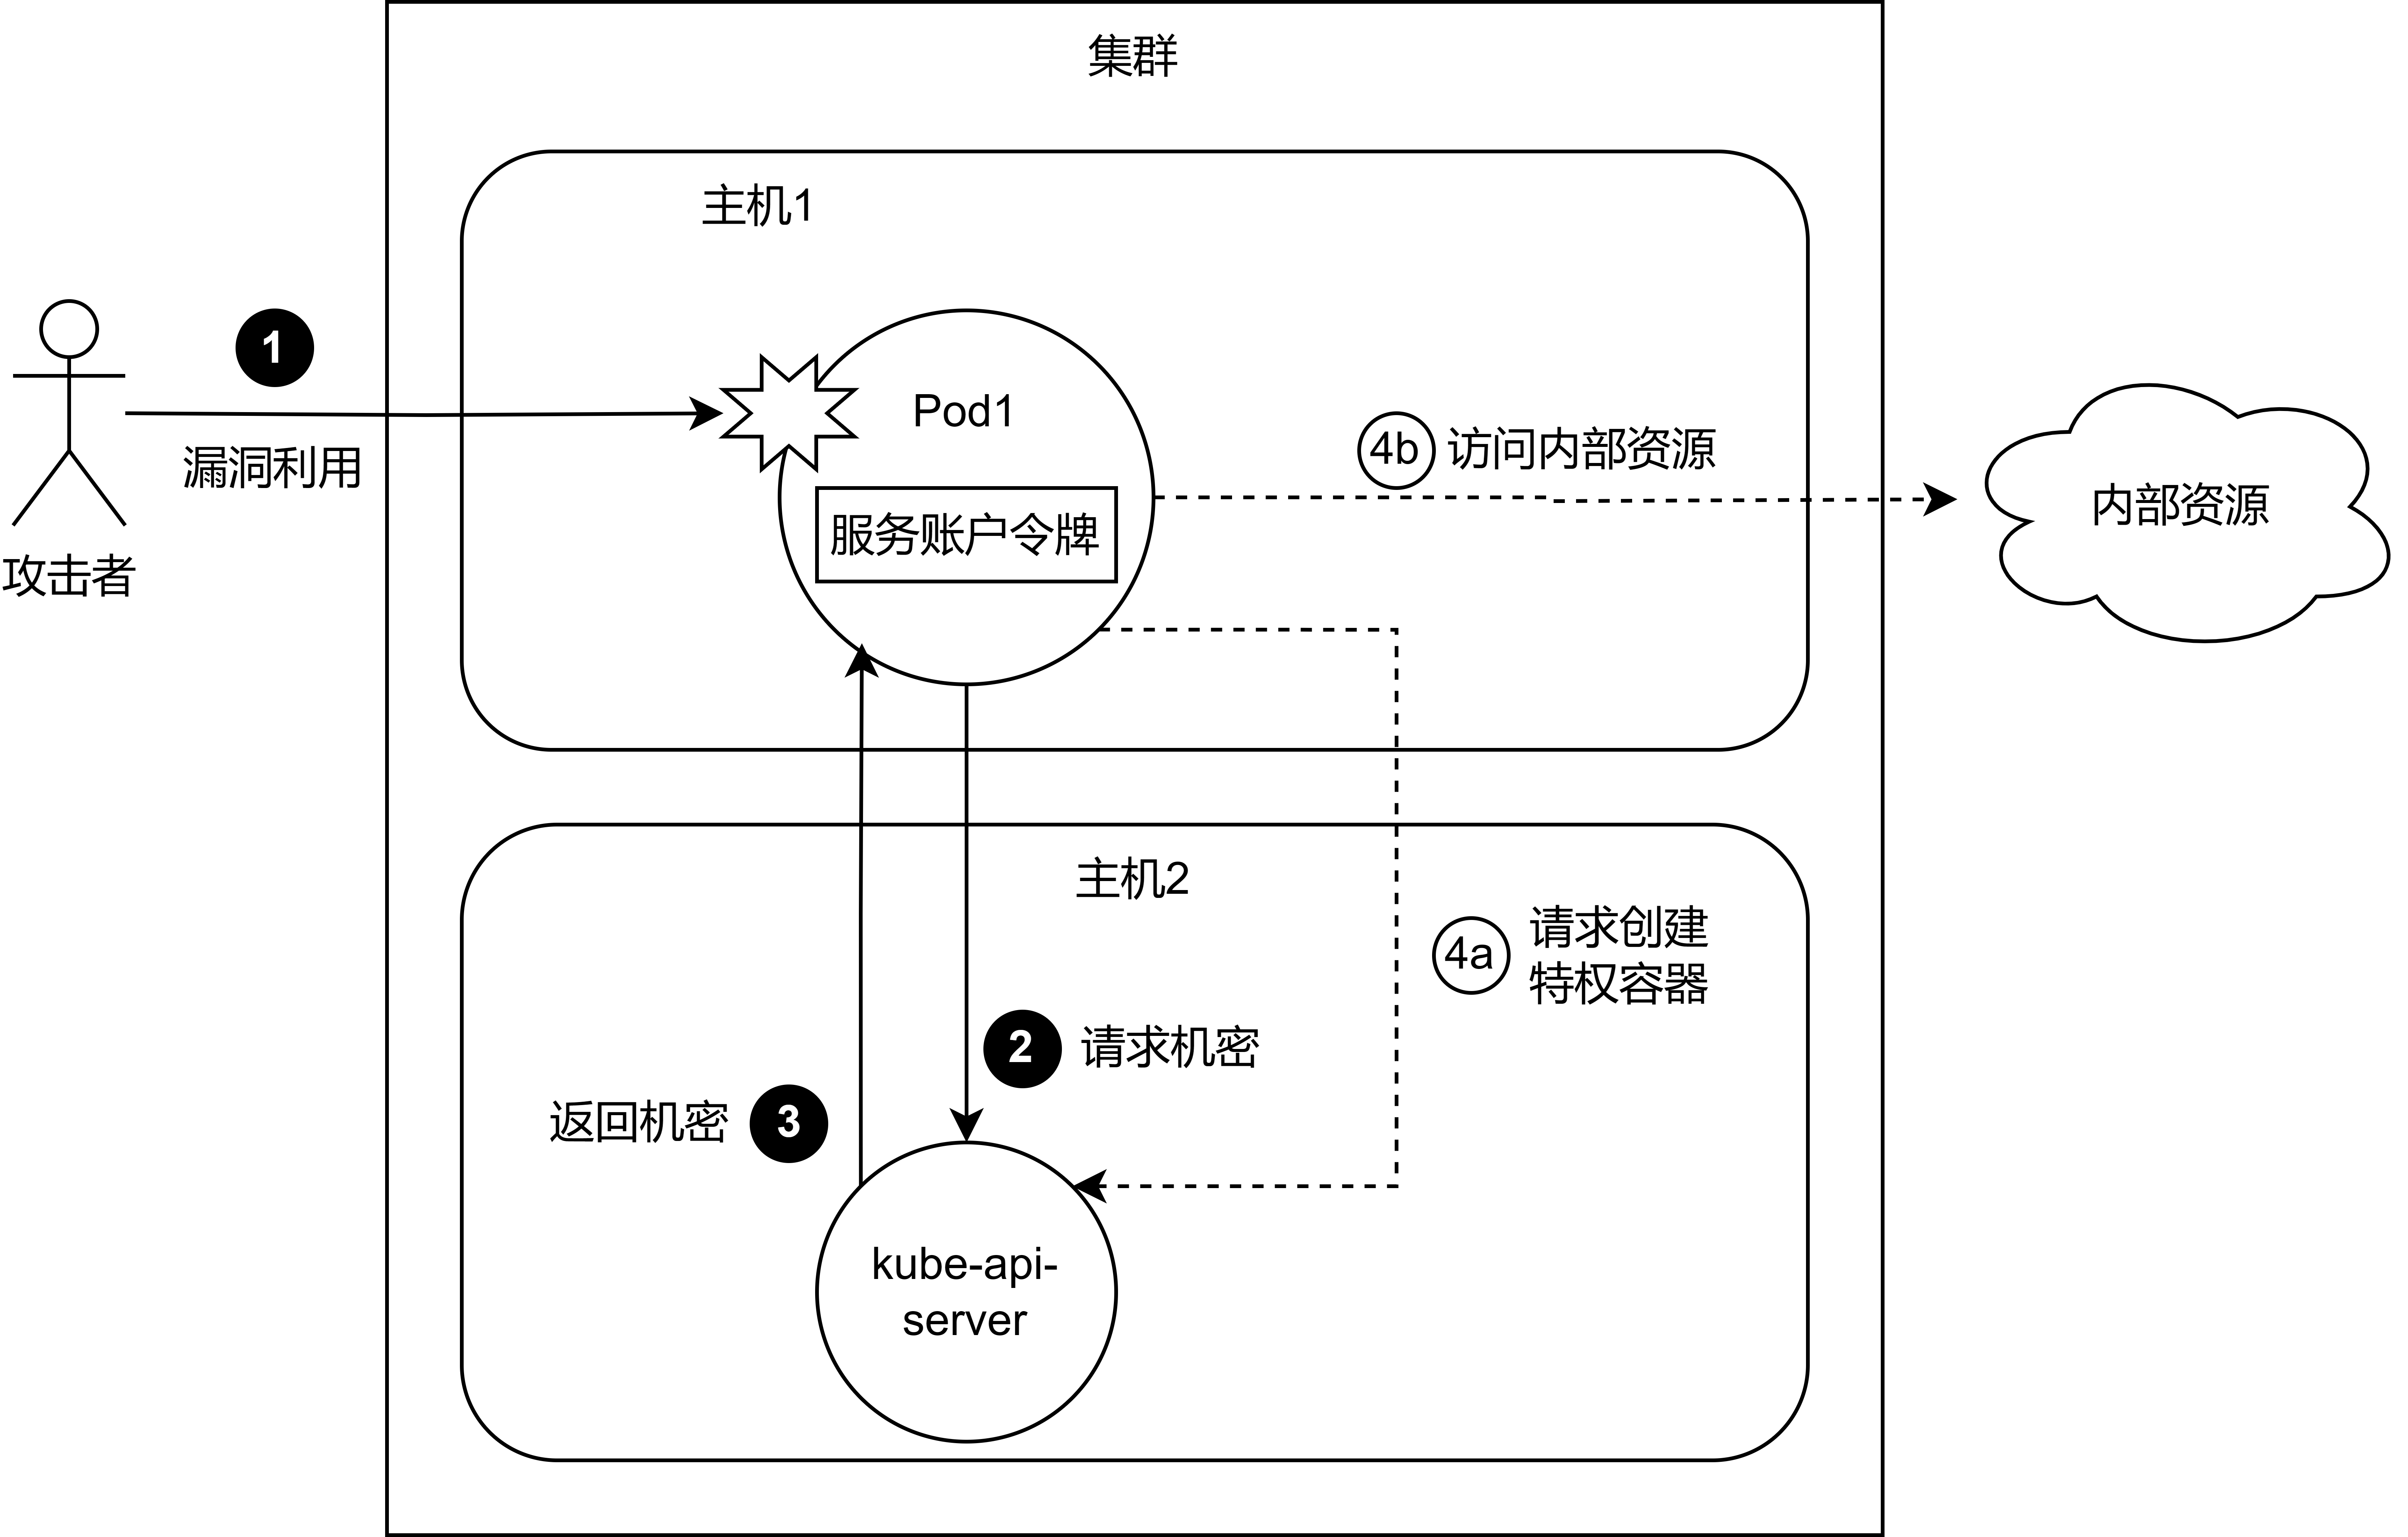
\includegraphics[width=0.95\textwidth]{attack-1}
    \bicaption{\enspace 容器化环境中的攻击链}{\enspace Attack Chain in Containerized Enviroments}
    \label{fig:attack-1}

\end{figure}

攻击链的各个阶段详细介绍如下:

\begin{enumerate}
    \item 攻击者进入目标集群。该阶段可通过远程代码执行漏洞实现,也可通过供应链攻击实现。攻击后,攻击者即可控制集群中的某个 Pod。
    \item 攻击者利用 Pod 中挂载的服务账户令牌,向集群 API 服务器请求身份认证。
    \item 集群 API 服务器对攻击者的身份认证通过。这是因为攻击者使用了 Pod 中的服务账户令牌,使 API 服务器不能识别攻击者的身份。
    \item 在这个阶段,攻击者尝试从当前的 Pod 移动到其他地方。图~\ref{fig:attack-1}~中给出了两个示例,其中第一个示例是创建一个新的特权 Pod,并将主机上的目录挂载到 Pod 中,从而实现从 Pod 到主机的横向移动;第二个示例是向 API 服务器请求机密信息,通过该机密信息,攻击者得以获得内部数据库等其他资源的访问权限。
\end{enumerate}

通过对攻击链的分析,本文发现,攻击者若要进行横向移动攻击,其最关键之处在于与 API 服务器之间的通信。攻击者需要与其通信,才能对集群的资源进行操作。因此,本文接下来将通过网络流量特征,对 API 服务器的异常通信进行检测,从而检测横向移动行为。

\section{基于网络流量特征的关键横向移动流检测方法}

本节基于网络流量特征检测关键横向移动流。检测流程如图~\ref{fig:detect-1}~所示。

\begin{figure}[!htbp]
    \centering
    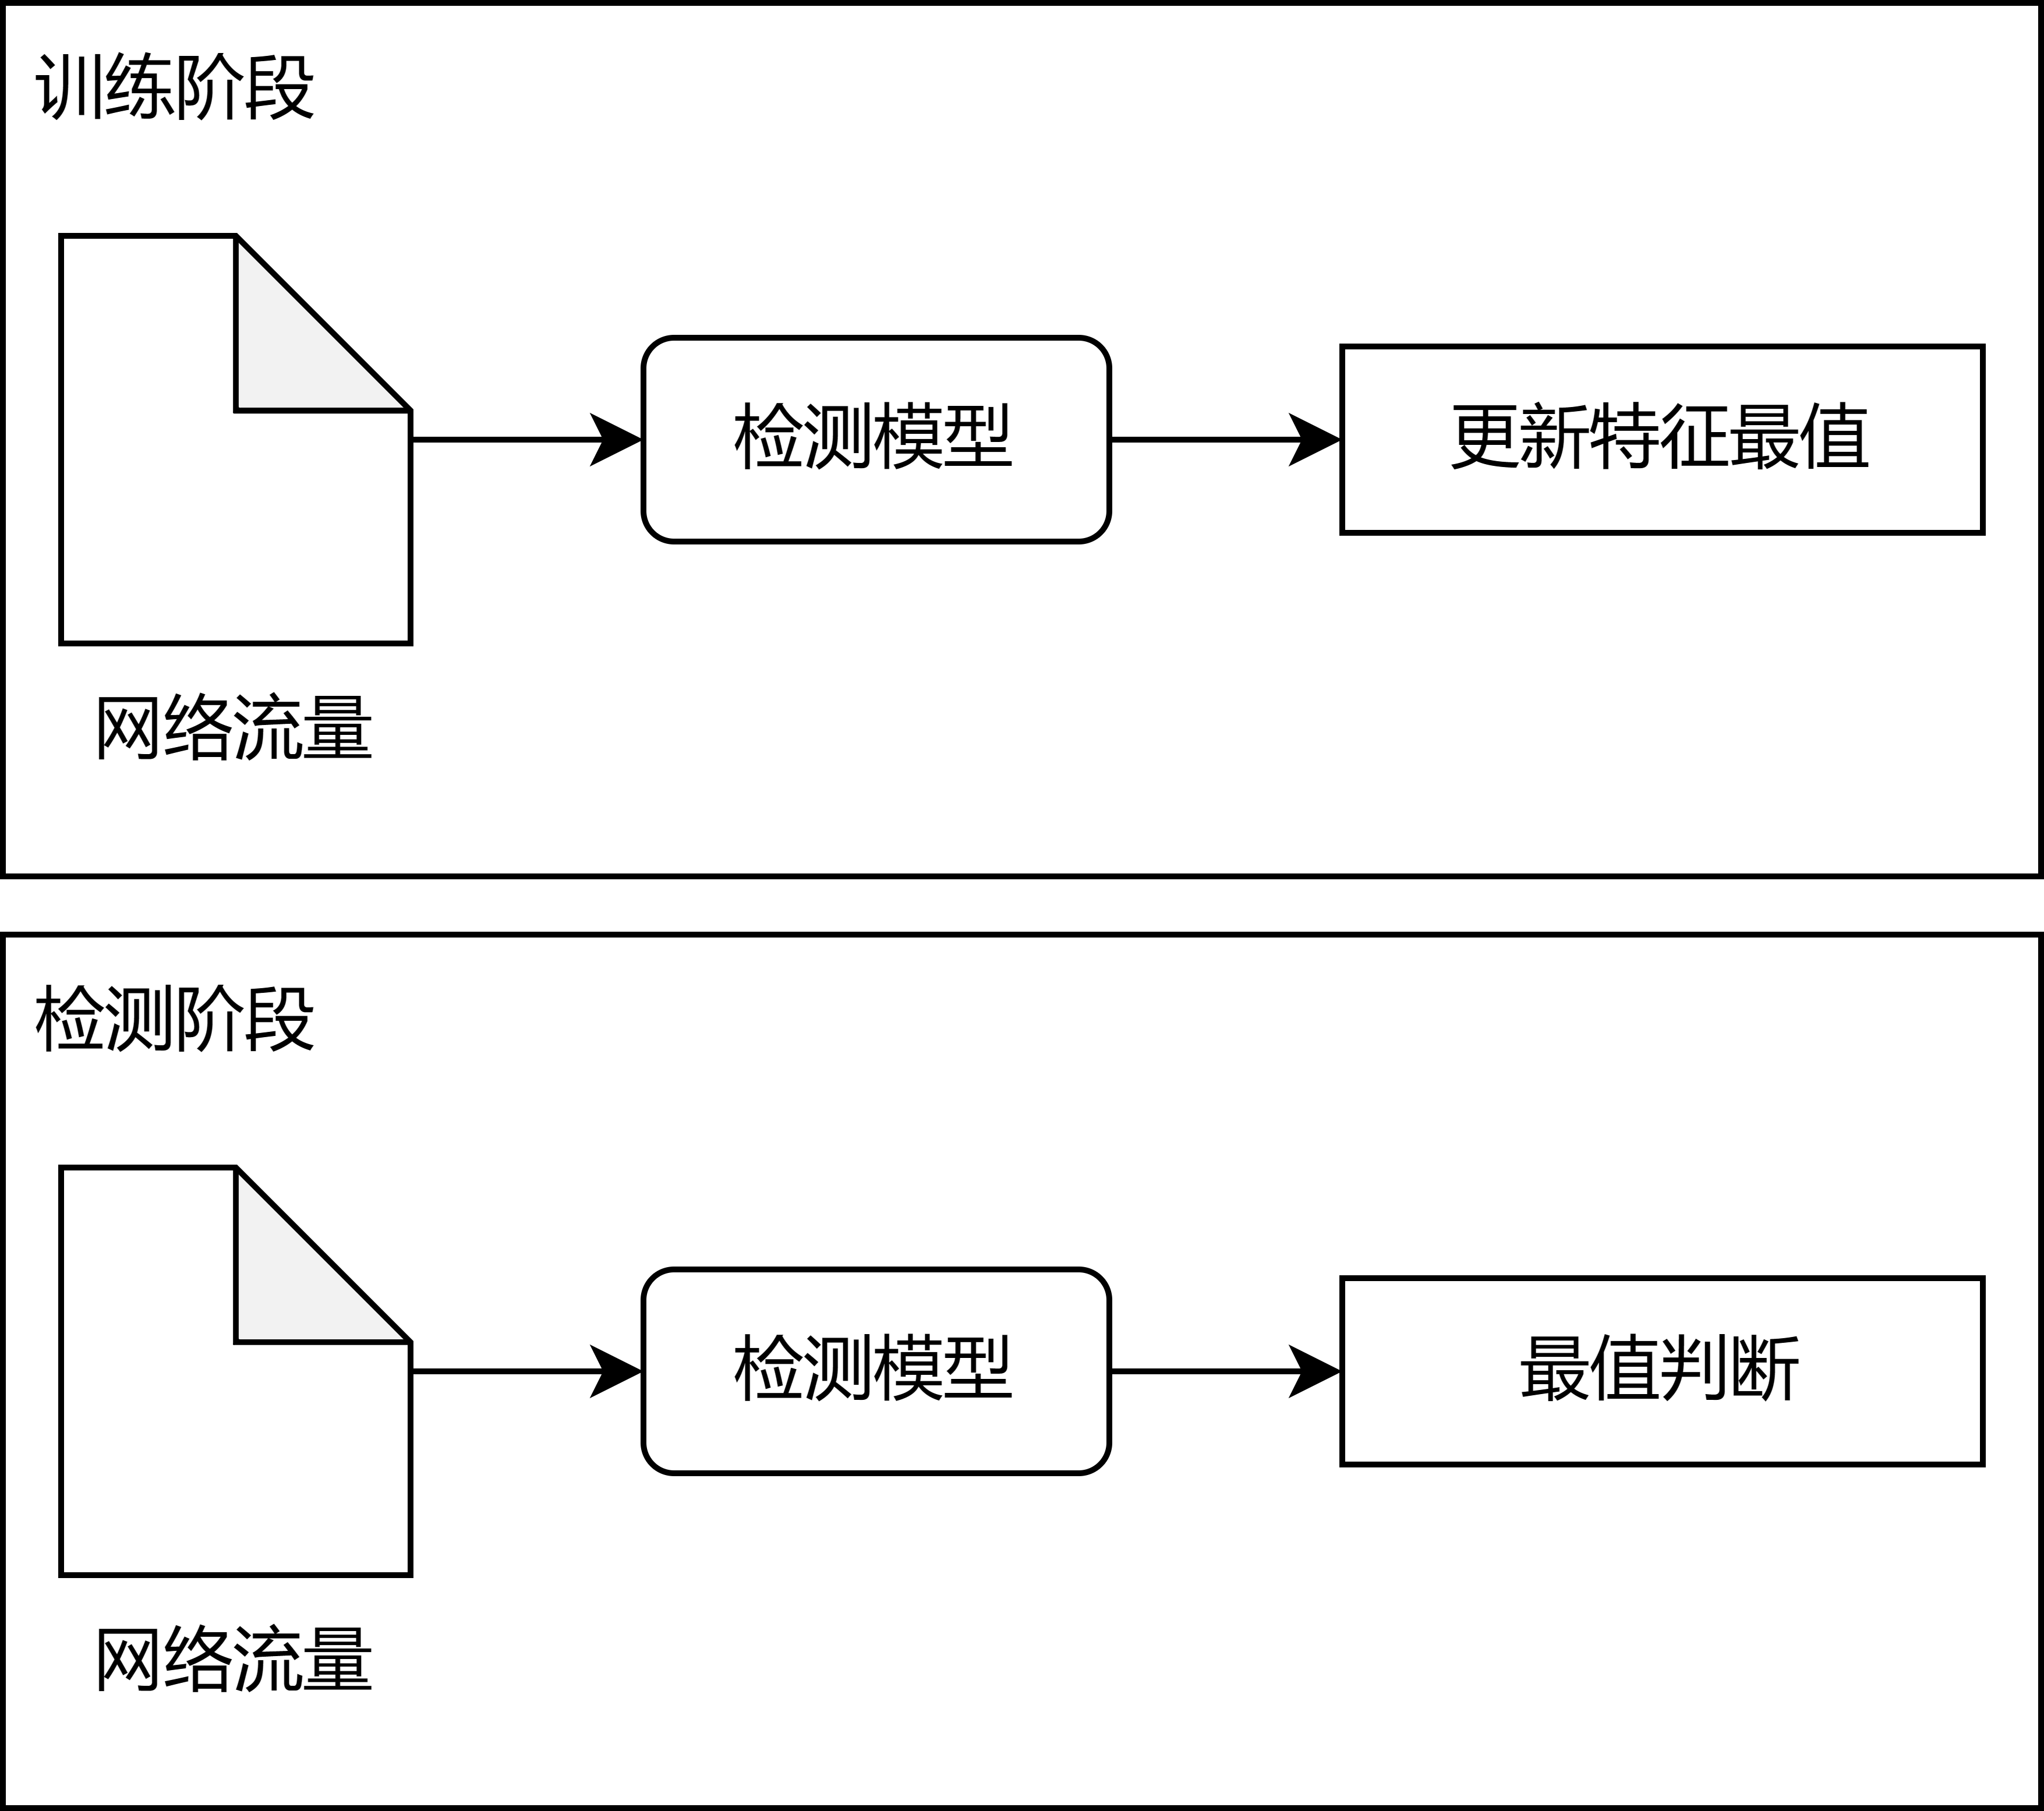
\includegraphics[width=0.50\textwidth]{detect-1}
    \bicaption{\enspace 基于网络流量特征的关键横向移动流检测流程}{\enspace Procedure of Detecting Key Flows of Lateral Movements by Flow Features}
    \label{fig:detect-1}

\end{figure}

该方法的基本思想是,当网络出现不同寻常的通信时,将报告异常。该方法通过特征最值来判断横向移动流。该方法分为两个阶段进行:

\begin{itemize}
    \item 训练阶段。在该阶段,读入网络流量的特征,更新网络流量特征的最值。
    \item 检测阶段。在该阶段,读入网络流量的特征,超出最值范围的判定为异常。
\end{itemize}

方法的伪代码如图~\ref{fig:detect-code}~所示。

\begin{figure}[!htbp]
    \centering
    \begin{subfigure}[b]{1.0\textwidth}
        \hrulefill
        \begin{algorithmic}[1]
            \Require NetflowList, FeatureList
            \Ensure MinMap, MaxMap
            \Function {TrainMap}{NetflowList, FeatureList}
                \State MinMap $\gets \emptyset$, MaxMap $\gets \emptyset$
                \For{Netflow \textbf{in} NetflowList}
                    \If{Netflow.SrcPort $\neq$ 6443 \textbf{or} Netflow.DstPort $\neq$ 6443}
                        \State \textbf{continue}
                    \EndIf
                    \For{Feature \textbf{in} FeatureList}
                        \State MinMap[Feature] $\gets $ Min (MinMap[Feature], Netflow[Feature])
                        \State MaxMap[Feature] $\gets $ Max (MinMap[Feature], Netflow[Feature])
                    \EndFor
                \EndFor
            \EndFunction
            \end{algorithmic}
        \hrulefill
        \caption{训练阶段}
    \end{subfigure}
    \\
    \begin{subfigure}[b]{1.0\textwidth}
        \hrulefill
            \begin{algorithmic}[1]
            \Require NetflowList, FeatureList, MinMap, MaxMap
            \Ensure Alerts
            \Function{TestFlow}{NetflowList, FeatureList, MinMap, MaxMap}
                \For{Netflow \textbf{in} NetflowList}
                    \If{Netflow.SrcPort $\neq$ 6443 \textbf{or} Netflow.DstPort $\neq$ 6443}
                        \State \textbf{continue}
                    \EndIf
                    \For{Feature \textbf{in} FeatureList}
                        \If{MinMap[Feature] $>$ Netflow[Feature] \textbf{or} MaxMap[Feature] $<$ Netflow[Feature]}
                            \State \textbf{alert} Netflow
                        \EndIf
                    \EndFor
                \EndFor
            \EndFunction
            \end{algorithmic}
        \hrulefill
        \caption{检测阶段}
    \end{subfigure}
    \bicaption{\enspace 基于网络流量特征的关键横向移动流检测伪代码}{\enspace Pseudocode of Detecting Key Flows of Lateral Movements}
    \label{fig:detect-code}
\end{figure}

\section{基于网络拓扑结构的关键横向移动流检测方法}

除了网络流量特征以外,攻击者的横向移动还会影响网络的拓扑结构。从容器化环境中的攻击链可以看出,攻击者可能通过新建特权 Pod 的形式实施 Pod 逃逸,以接管主机。在容器化集群中,每个 Pod 对应一个 IP 地址,因此新增 Pod 时,也会新增一个 IP 地址,从而更改了网络的拓扑结构。

此外,当攻击者攻破某一个 Pod 时,为了方便控制该 Pod,常用的方式是使用命令与控制服务器(Command and Control,C\&C)与该 Pod 进行通信。因此,该 Pod 将向其以前从未访问过的 IP 地址传输数据,从而更改了网络的拓扑结构。

因此,本文提出基于网络拓扑结构的关键横向移动流检测方法,检测流程如图~\ref{fig:detect-2}~所示。

\begin{figure}[!htbp]
    \centering
    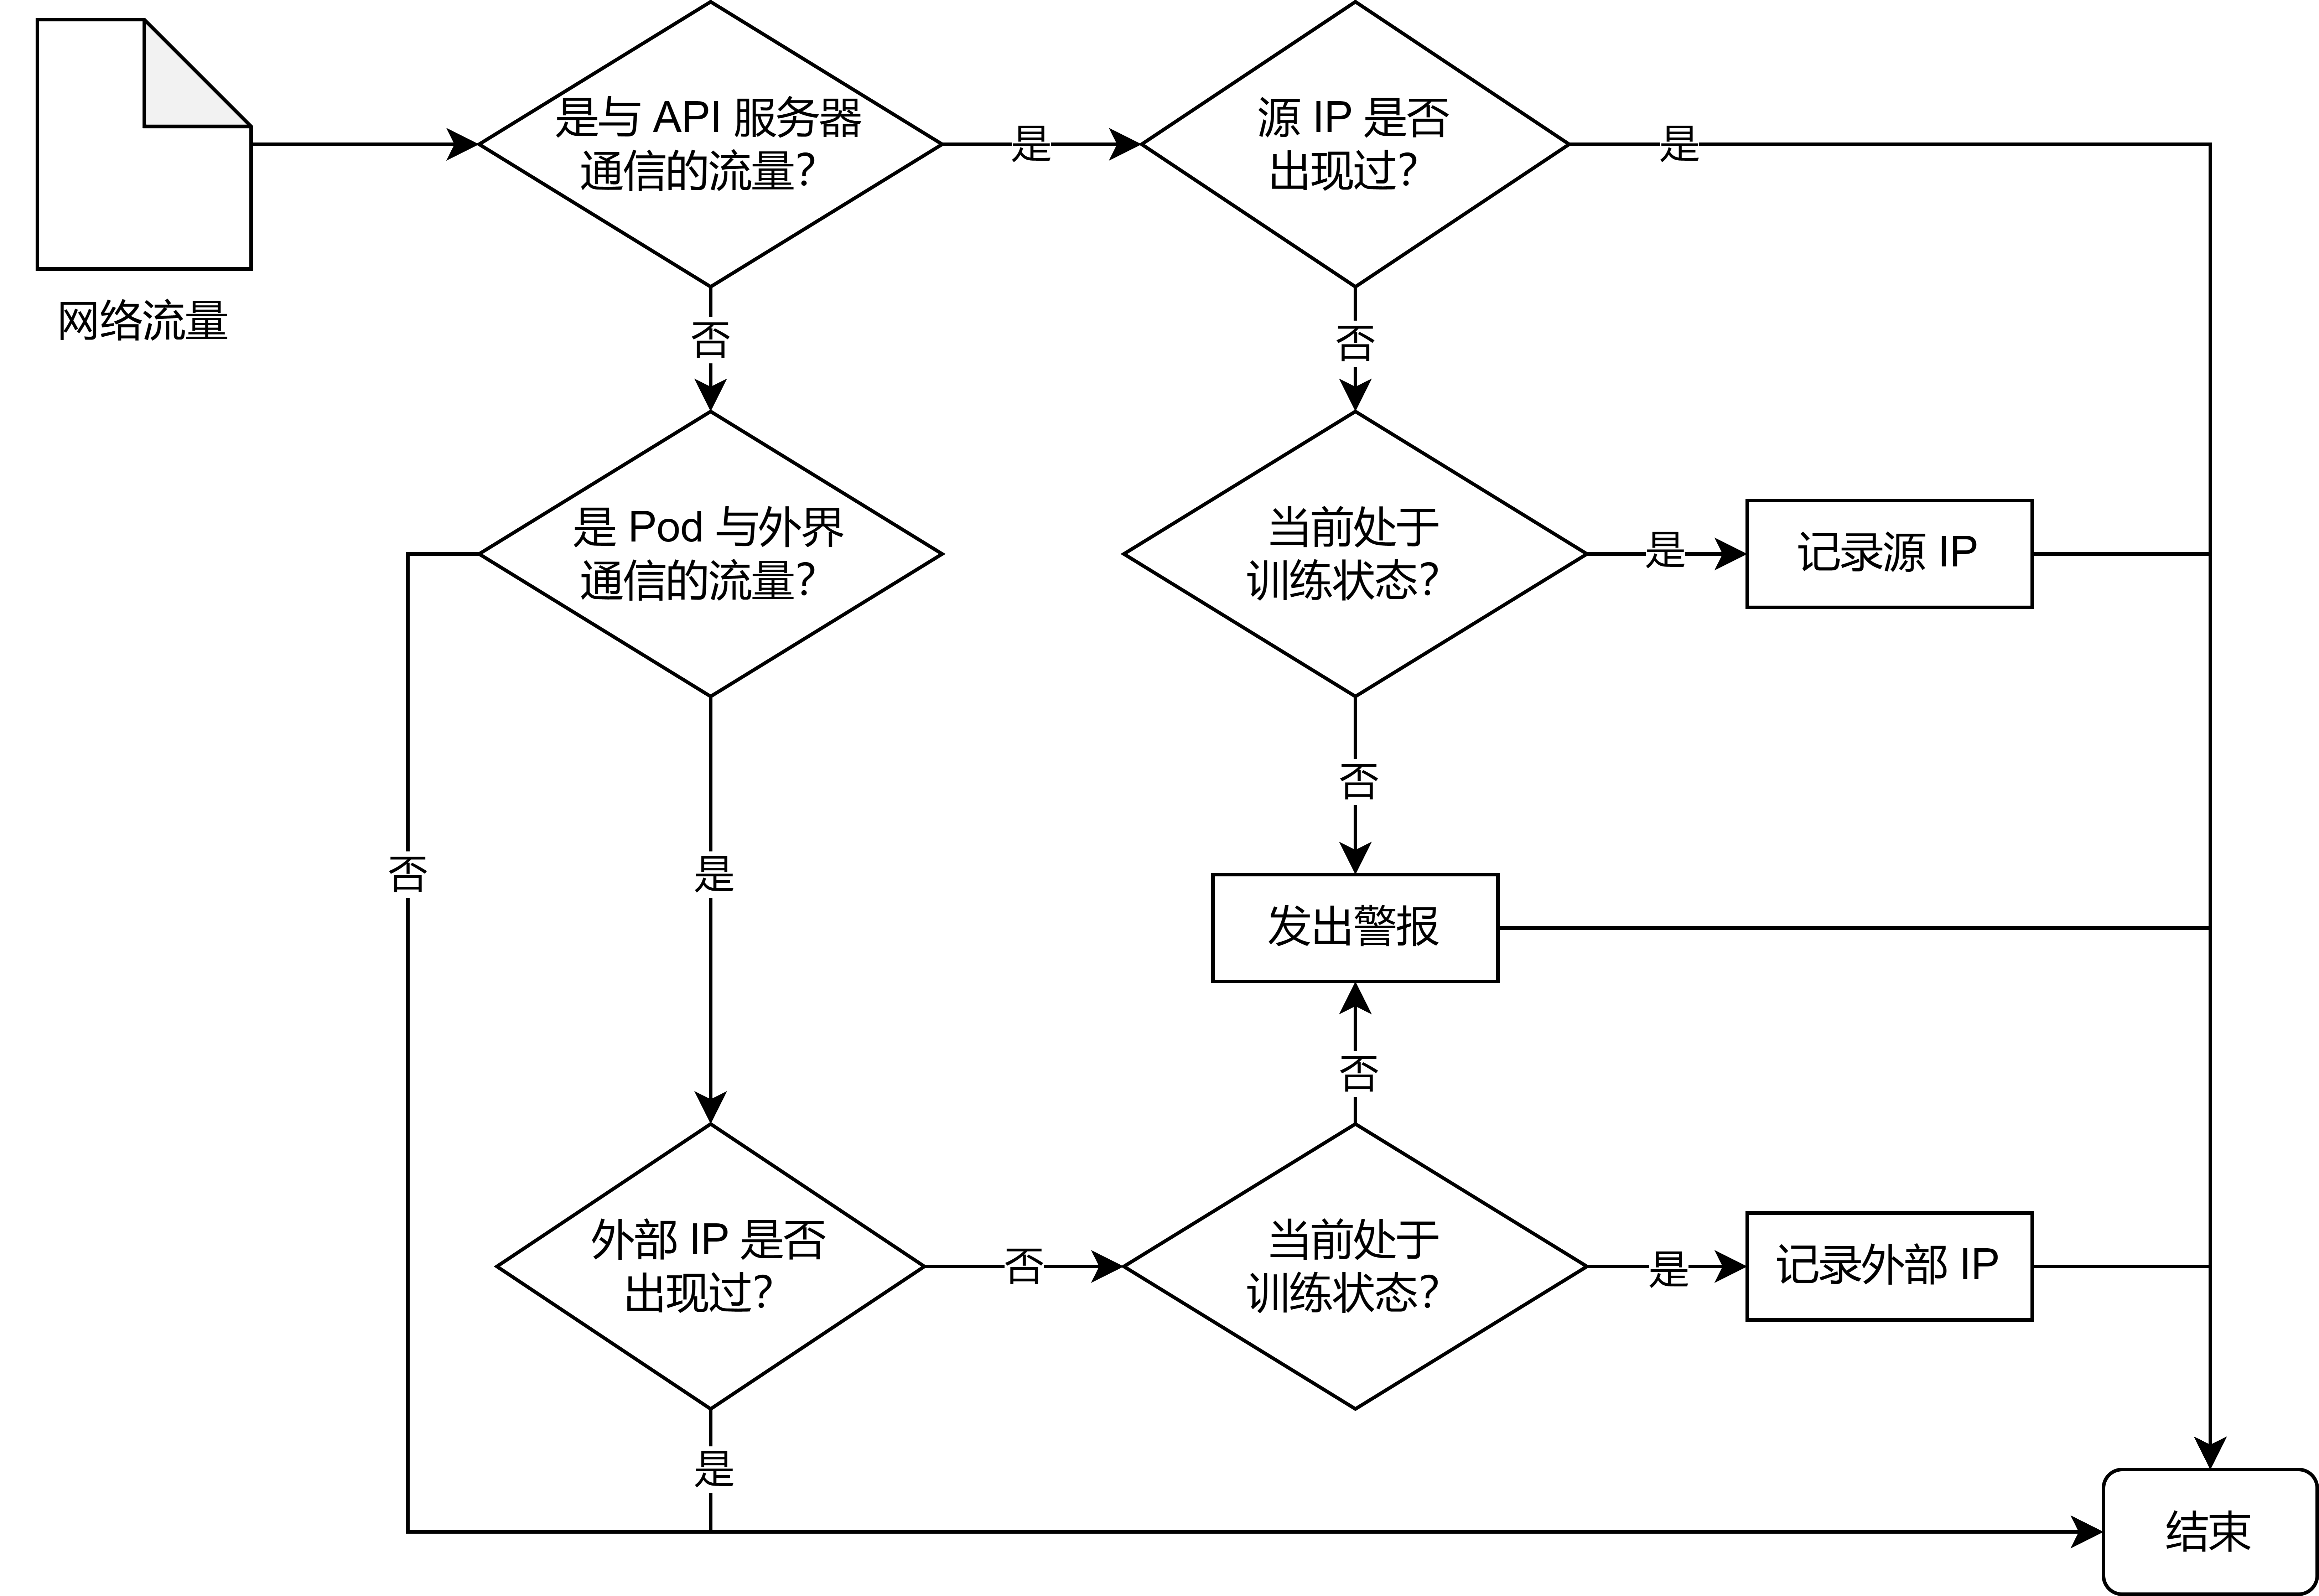
\includegraphics[width=1.0\textwidth]{detect-2}
    \bicaption{\enspace 基于网络拓扑结构的关键横向移动流检测流程}{\enspace Procedure of Detecting Key Flows of Lateral Movements by Topology}
    \label{fig:detect-2}

\end{figure}

其基本流程如下:

\begin{enumerate}
    \item 对于 API 服务器的通信,在训练阶段,记录通信的源 IP 地址;在检测阶段,检查通信的源 IP 地址是否在已记录的范围内,若未记录,则发出警报;
    \item 对于 Pod 与外部网络之间的通信,在训练阶段,记录通信的外部 IP 地址;在检测阶段,检查通信的外部 IP 地址是否在已记录的范围内,若未记录,则发出警报。
\end{enumerate}

实际应用时,根据具体部署的应用,可以对上述方法作适当调整,例如对于 Pod 与外部网络的通信,可以用域名来取代外部 IP 地址,使其更加准确;对于不需要与外部网络通信的 Pod,则可以简化策略,无需再训练阶段记录,而是在检测阶段直接检查该 Pod 是否与外部网络发生了通信,若发生了通信,则发出警报。

\section{数据集分析和验证}

本节使用 Kubernetes-dataset 数据集对关键横向移动流检测方法进行验证,其详细介绍见第~\ref{sec:dataset}~节。

\subsection{基于网络流量特征的方法验证}

Kubernetes-dataset 数据集中包含的网络流特征如表 ~\ref{tab:dataset-features}~ 所示。

\begin{table}[!htbp]
    \bicaption{\enspace Kubernetes-dataset 数据集包含的特征}{\enspace Features in Kubernetes-dataset}
    \label{tab:dataset-features}
    \centering
    \footnotesize% fontsize
    \setlength{\tabcolsep}{4pt}% column separation
    \renewcommand{\arraystretch}{1.2}%row space 
    \begin{tabular}{cp{10cm}c}
        \hline
        特征类别 & 特征 & 维度\\
        \hline
        流持续时间 & 流持续毫秒数、TCP流持续毫秒数 & 2\\
        数据包的数量 & 前向数据包数量、后向数据包数量、后向与前向数据包比例、含有至少1字节数据的数据包数量 & 4\\
        数据包的长度 & 前向数据包总长度、后向数据包总长度、前向数据包长度最大值、前向数据包长度最小值、前向数据包长度平均值、前向数据包长度标准差、后向数据包长度最大值、后向数据包长度最小值、后向数据包长度平均值、后向数据包长度标准差、数据包长度最小值、数据包长度最大值、数据包长度平均值、数据包长度标准差、数据包长度方差、平均数据包长度、前向数据段平均大小、后向数据段平均大小、前向数据段最小值 & 19\\
        流速 & 流速(包/秒)、流速(字节/秒)、前向流速(包/秒)、后向流速(包/秒)& 4\\
        数据包的间隔 & 数据包到达时间间隔(IAT)平均值、IAT标准差、IAT最大值、IAT最小值、前向IAT总和、前向IAT平均值、前向IAT标准差、前向IAT最大值、前向IAT最小值、后向IAT总和、后向IAT平均值、后向IAT标准差、后向IAT最大值、后向IAT最小值 & 14\\
        TCP Flag统计 & 前向PSH、后向PSH、前向URG、后向URG、前向RST、后向RST、FIN、SYN、RST、PSH、ACK、URG、CWR、ECE & 14\\
        数据包首部 & 前向首部长度、后向首部长度 & 2\\
        批量(bulk)传输 & 前向每bulk传输字节数、前向每bulk传输数据包数、前向bulk速率、后向每bulk传输字节数、后向每bulk传输数据包数、后向bulk速率	& 6\\
        MPTCP子流 & 前向子流数据包数、前向子流字节数、后向子流数据包数、后向子流字节数	& 4\\
        TCP窗口 & 前向窗口初始值、后向窗口初始值 & 2\\
        活跃与空闲 & 连续活跃时长平均值、连续活跃时长标准差、连续活跃时长最大值、连续活跃时长最小值、连续空闲时长平均值、连续空闲时长标准差、连续空闲时长最大值、连续空闲时长最小值 & 8\\
        \hline
    \end{tabular}
\end{table}

将数据集中的各个特征用散点图画出,可得到良性流量与横向移动流量各特征的分布情况。可以发现,部分特征在横向移动流量的值域大于良性流量的值域。符合这类分布的特征包括:前向每 bulk 传输字节数、前向每 bulk 传输数据包数、前向 bulk 速率。以前向每 bulk 传输字节数为例,横向移动流量和良性流量的散点图如图~\ref{fig:flow-bytes-bulk-avg}~所示。

\begin{figure}[!htbp]
    \centering
    \begin{subfigure}[b]{0.48\textwidth}
      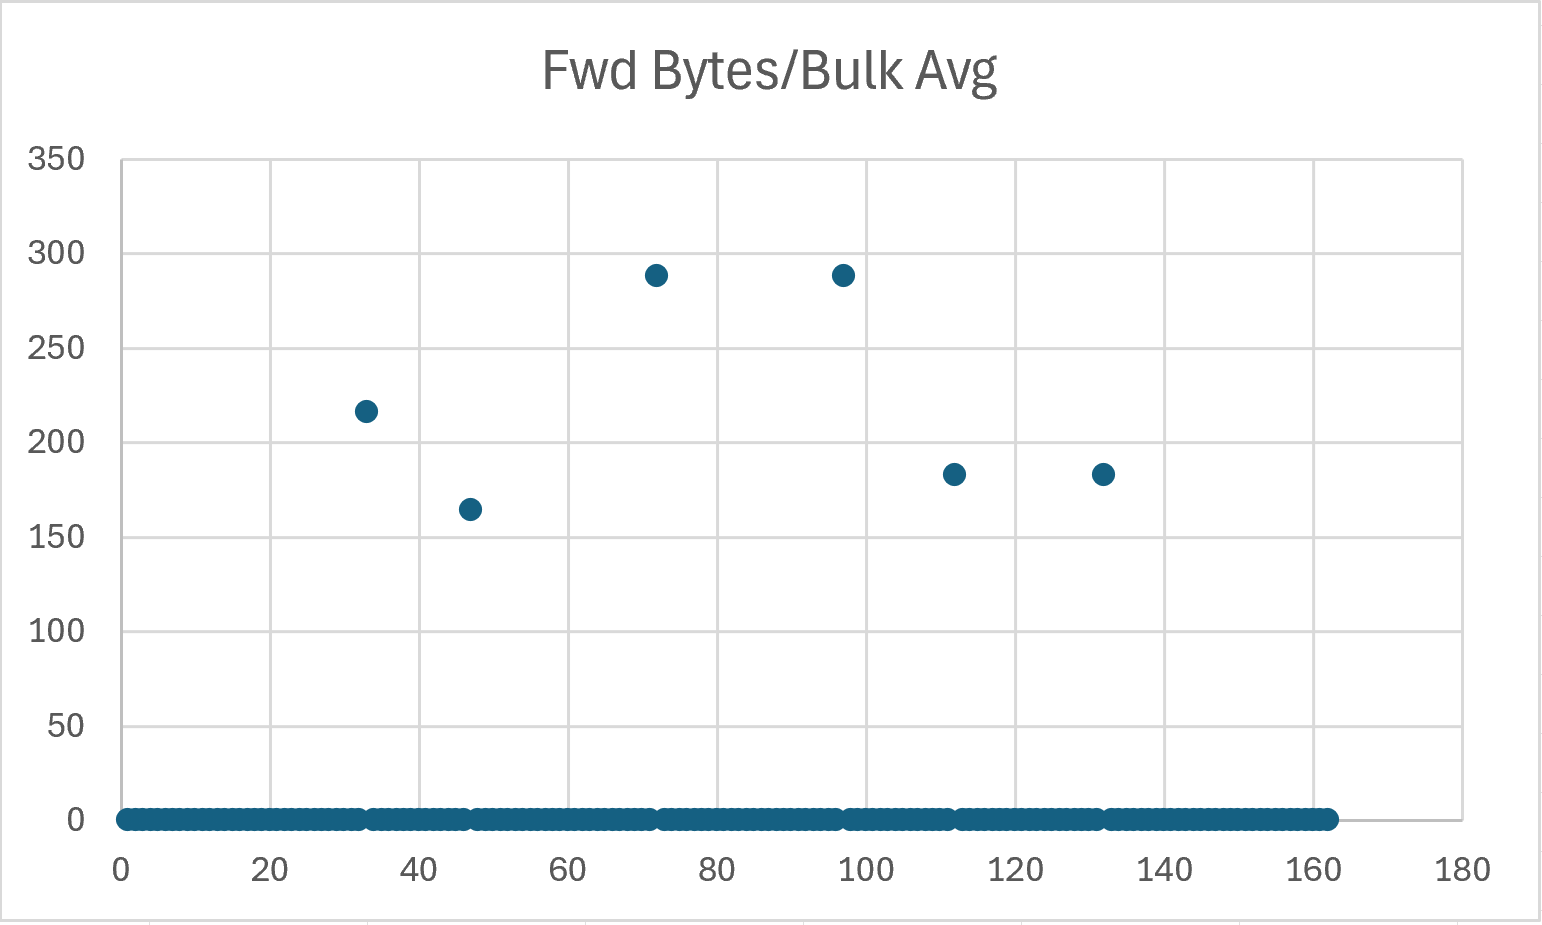
\includegraphics[width=\textwidth]{fwd-bytes-bulk-attack-1}
      \caption{横向移动流}
    \end{subfigure}%
    ~% add desired spacing
    \begin{subfigure}[b]{0.48\textwidth}
      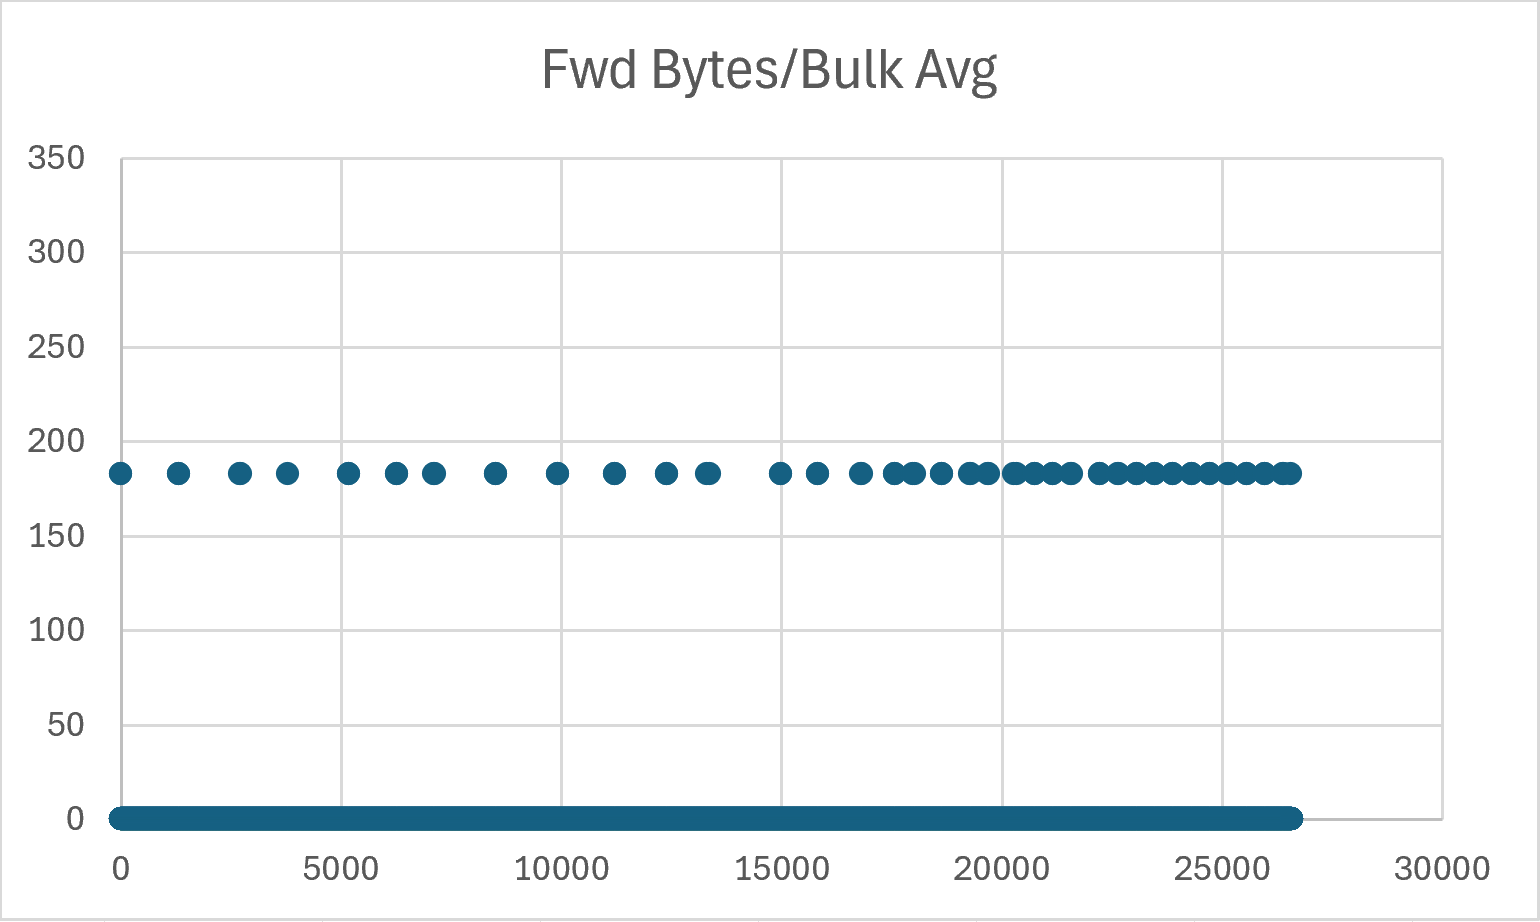
\includegraphics[width=\textwidth]{fwd-bytes-bulk-benign-1}
      \caption{良性流}
    \end{subfigure}
    \bicaption{\enspace 前向每 bulk 平均传输字节数散点图}{\enspace Scatterplot of Flow Bytes/bulk Average}
    \label{fig:flow-bytes-bulk-avg}
\end{figure}

在数据集中,若 TCP 流传输了大量数据,需分为多个数据包传输,这些数据包的集合就被称为 bulk。在进行流的聚合和特征提取时,CICFlowMeter 首先根据流中各数据包的发送时间间隔判断这些数据包能否被聚合为 bulk,然后统计数据包的数量,当数据包达到 4 个时就开始提取 bulk 的特征。因此,数据集中与 bulk 相关的特征通常为 $0$,仅在传输数据量较大时大于 $0$,表示此流发生了分包传输。

在图~\ref{fig:flow-bytes-bulk-avg}~所示的横向移动流中,共有$7$个流的前向数据发生了分包传输。这$7$个流的源IP地址、源端口、目标IP地址、目标端口如表~\ref{tab:dataset-malicious-bulks}~所示。

\begin{table}[!htbp]
    \bicaption{\enspace 横向移动流中发生分包传输的流}{\enspace Malicious Flows that Has Bulks}
    \label{tab:dataset-malicious-bulks}
    \centering
    \footnotesize% fontsize
    \setlength{\tabcolsep}{4pt}% column separation
    \renewcommand{\arraystretch}{1.2}%row space 
    \begin{tabular}{ccccccc}
        \hline
        编号 & 前向每 bulk 传输字节数 & 源 IP 地址 & 源端口 & 目标 IP 地址 & 目标端口 & 能否被检测出?\\
        \hline
        1 & 183 & 10.16.0.6 & 34788 & 144.122.71.18 & 6443 & 否\\
        2 & 183 & 10.16.0.2 & 56026 & 144.122.71.18 & 6443 & 否\\
        3 & 216 & 10.16.0.45 & 45956 & 144.122.71.18 & 6443 & 是\\
        4 & 164 & 10.16.0.45 & 47002 & 144.122.71.18 & 6443 & 是\\
        5 & 288 & 10.16.0.45 & 52904 & 144.122.71.18 & 6443 & 是\\
        6 & 288 & 10.16.0.45 & 52906 & 144.122.71.18 & 6443 & 是\\
        \hline
    \end{tabular}
\end{table}

与此同时,在良性流中,“前向每 bulk 传输字节数”大于 0 的流的情况如表~\ref{tab:dataset-benign-bulks}~所示。其中,具有相同或相似(除源端口以外其他特征相同)特征的流仅展示一次。

\begin{table}[!htbp]
    \bicaption{\enspace 良性流中发生分包传输的流}{\enspace Benign Flows that Has Bulks}
    \label{tab:dataset-benign-bulks}
    \centering
    \footnotesize% fontsize
    \setlength{\tabcolsep}{4pt}% column separation
    \renewcommand{\arraystretch}{1.2}%row space 
    \begin{tabular}{cccccc}
        \hline
        编号 & 前向每 bulk 传输字节数 & 源 IP 地址 & 源端口 & 目标 IP 地址 & 目标端口\\
        \hline
        7 & 183 & 10.16.0.6 & 34788 & 144.122.71.18 & 6443\\
        8 & 183 & 10.16.0.2 & 56026 & 144.122.71.18 & 6443\\
        \hline
    \end{tabular}
\end{table}

留意到良性流量中,向该端口传输数据的流的“前向每 bulk 传输字节数”通常为 183 字节,但横向移动流中出现了不同的值,说明 API 服务器接收到了与以往不相同的指令,而这正是横向移动攻击的关键。通过与 API 服务器通信,攻击者可以执行创建、更新、删除容器化集群中的 Pod 等资源,或者控制集群的行为,例如滚动更新、扩缩容等。因此,编号为 3、4、5、6 的 $4$ 个关键的横向移动流可通过此特征检测出来。

除了与 bulk 相关的特征以外,前向发送数据量、前向 PSH、前向首部长度等特征也可将这些流检测出来。

通过上述验证,本文证明了通过最值验证,可以检测出攻击者对 API 服务器的恶意操作,这是横向移动中的关键步骤。

(二)横向移动流量的值域与良性流量的值域大致相同。与IAT相关的特征,SYN、RST、FIN等与TCP协议握手、挥手过程相关的特征,前向初始窗口,前向数据段最小值属于此类。以IAT平均值为例,横向移动流和良性流的散点图如图~\ref{fig:flow-iat-mean}~所示。

\begin{figure}[!htbp]
    \centering
    \begin{subfigure}[b]{0.48\textwidth}
      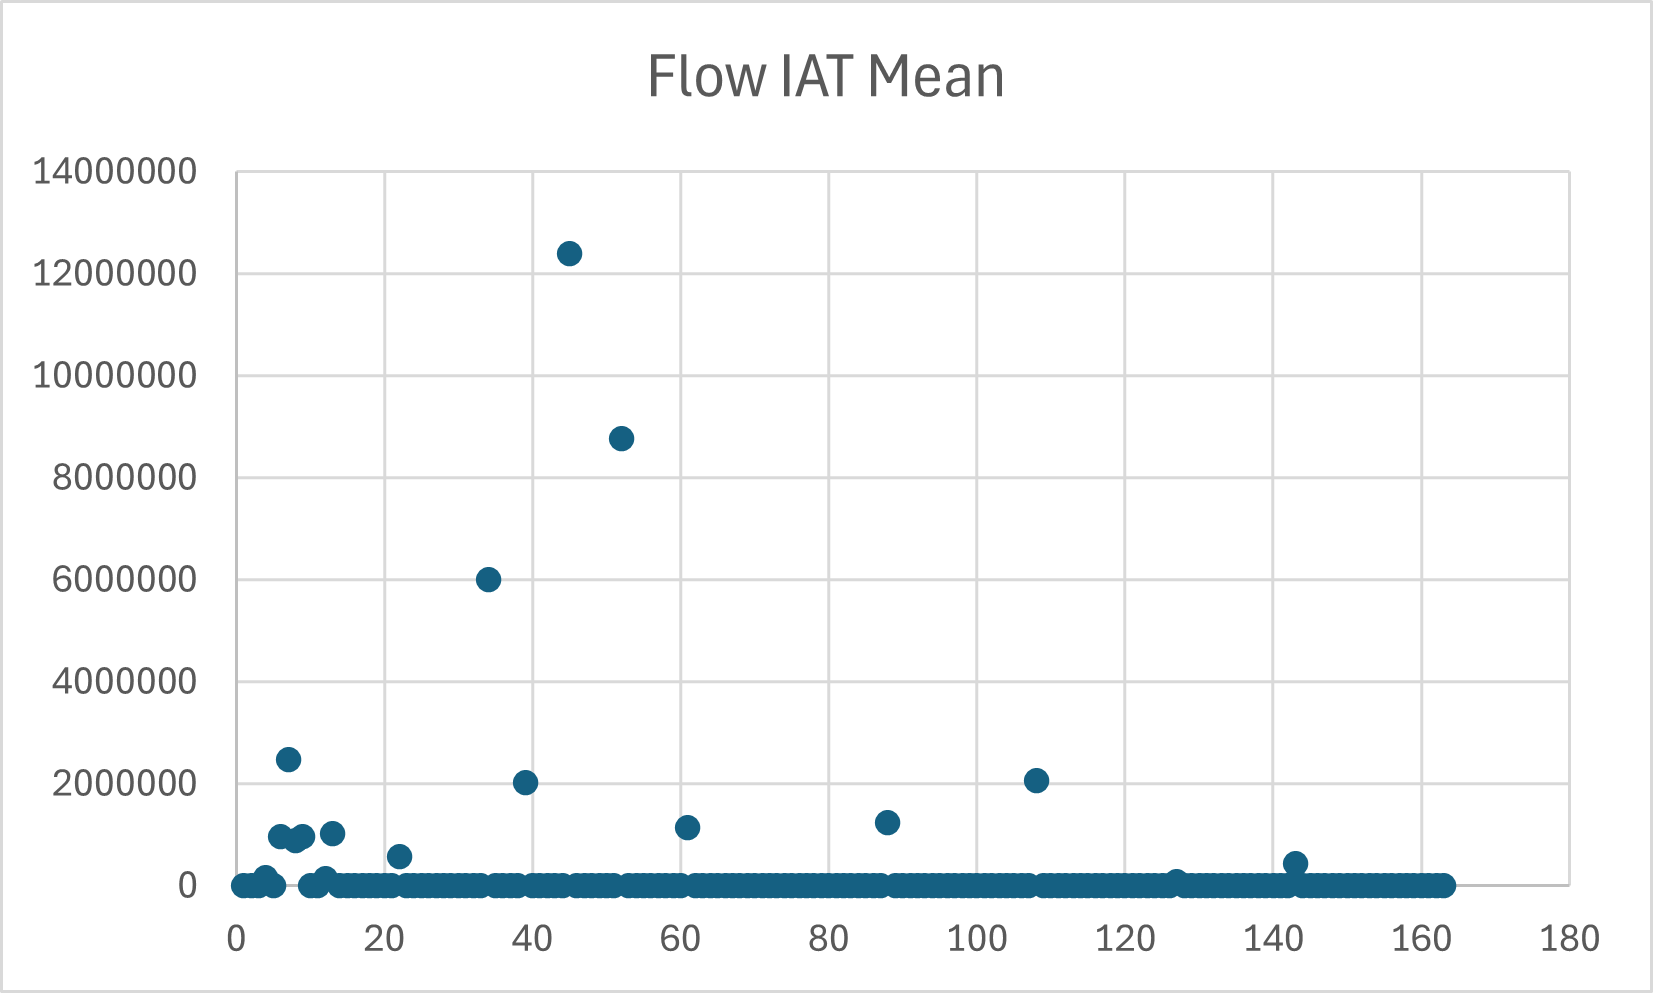
\includegraphics[width=\textwidth]{flow-iat-mean-attack}
      \caption{横向移动流}
    \end{subfigure}%
    ~% add desired spacing
    \begin{subfigure}[b]{0.48\textwidth}
      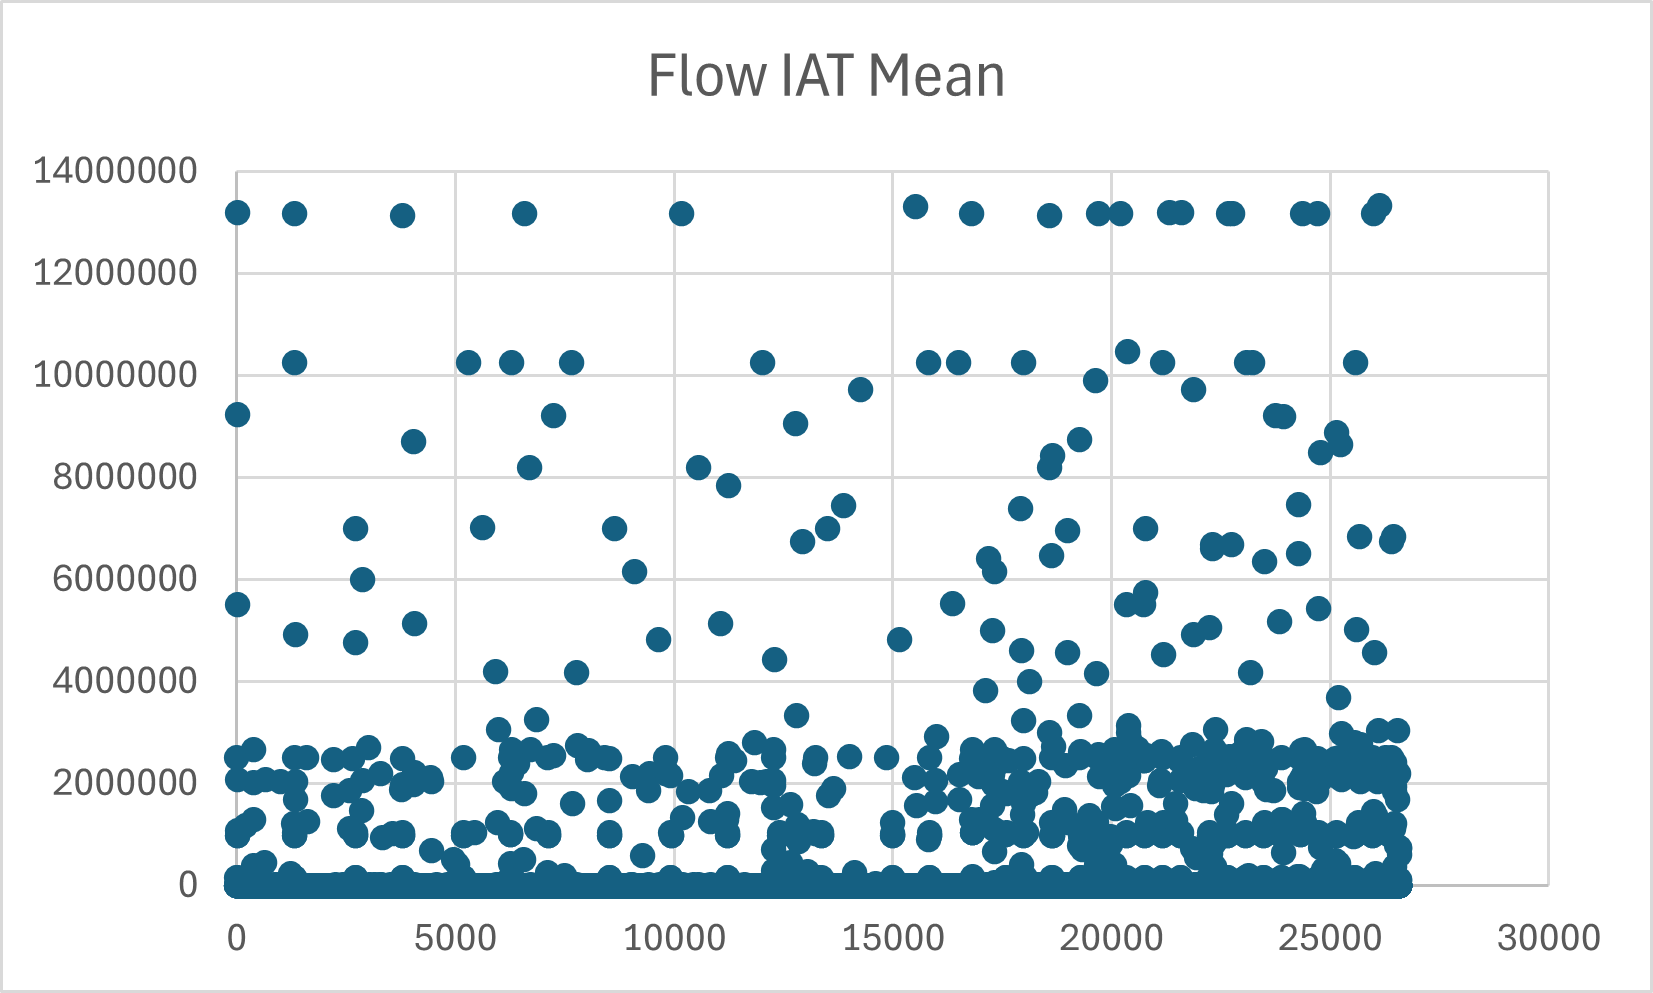
\includegraphics[width=\textwidth]{flow-iat-mean-benign}
      \caption{良性流}
    \end{subfigure}
    \bicaption{\enspace IAT 平均值散点图}{\enspace Scatterplot of IAT Mean}
    \label{fig:flow-iat-mean}
\end{figure}

此类特征难以区分横向移动流和良性流,因此难以直接用来识别横向移动。

(三)横向移动流量的值域小于良性流量的值域。与流持续时间、流速、包长相关且没有在(一)中讨论的特征属于此类。以流速为例,横向移动流量和良性流量的散点图如图~\ref{fig:flow-bytes}~所示。

\begin{figure}[!htbp]
    \centering
    \begin{subfigure}[b]{0.48\textwidth}
      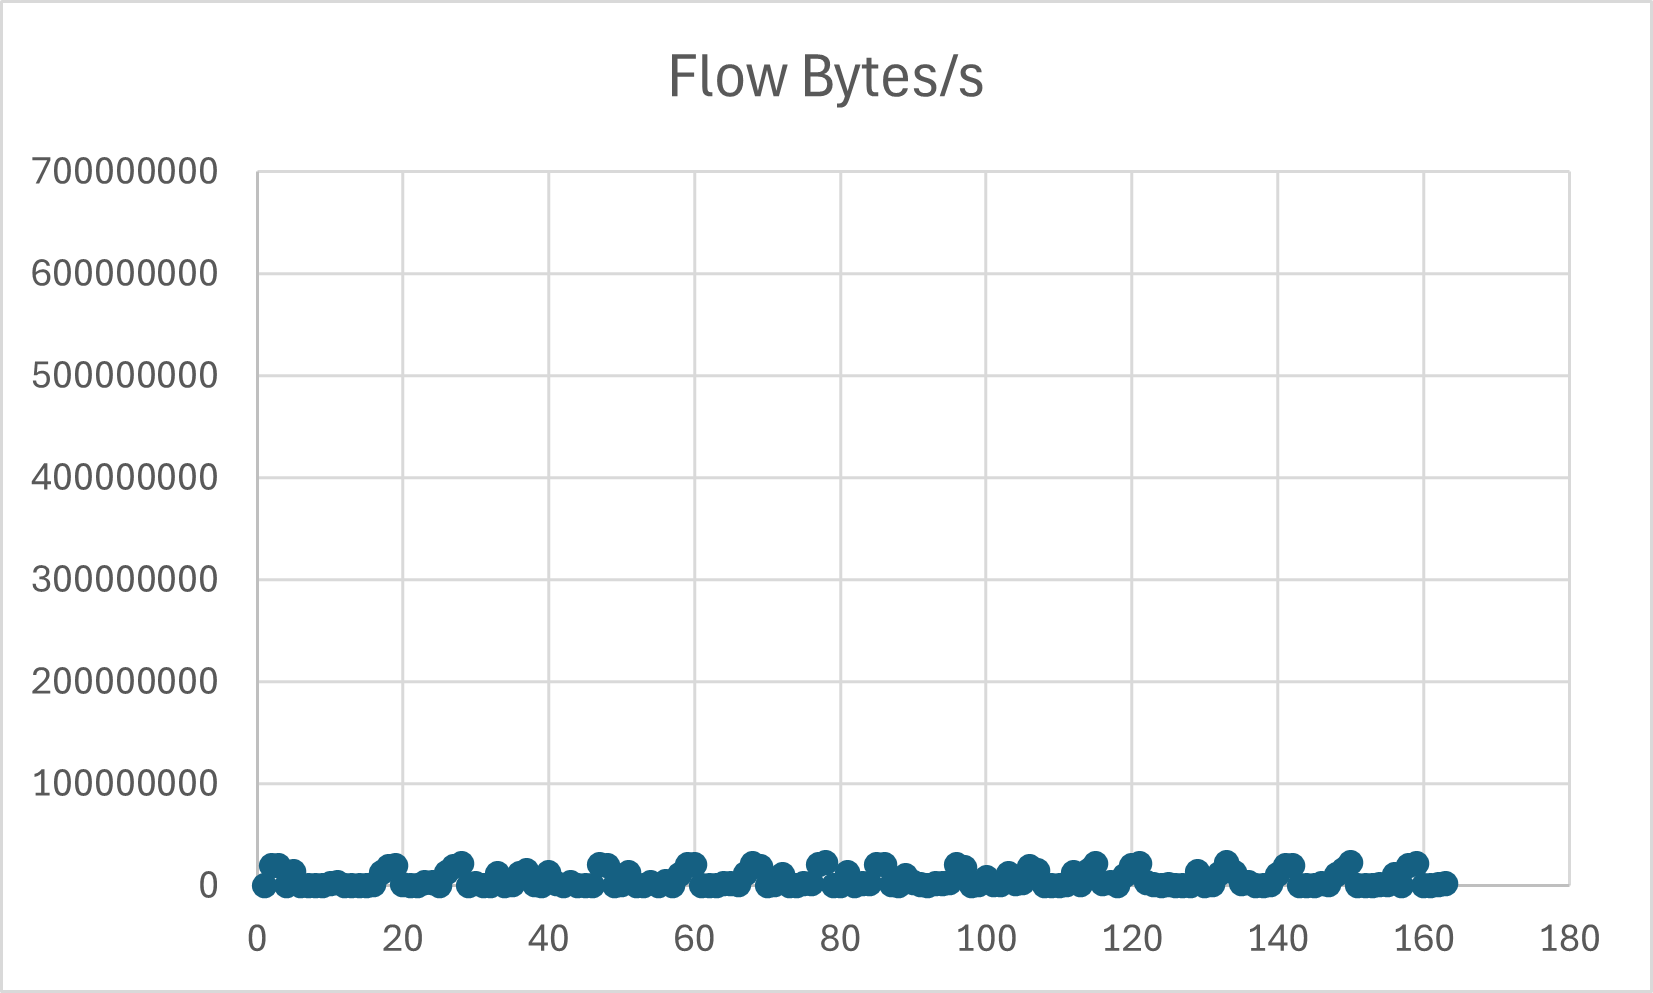
\includegraphics[width=\textwidth]{flow-bytes-attack}
      \caption{横向移动流}
    \end{subfigure}%
    ~% add desired spacing
    \begin{subfigure}[b]{0.48\textwidth}
      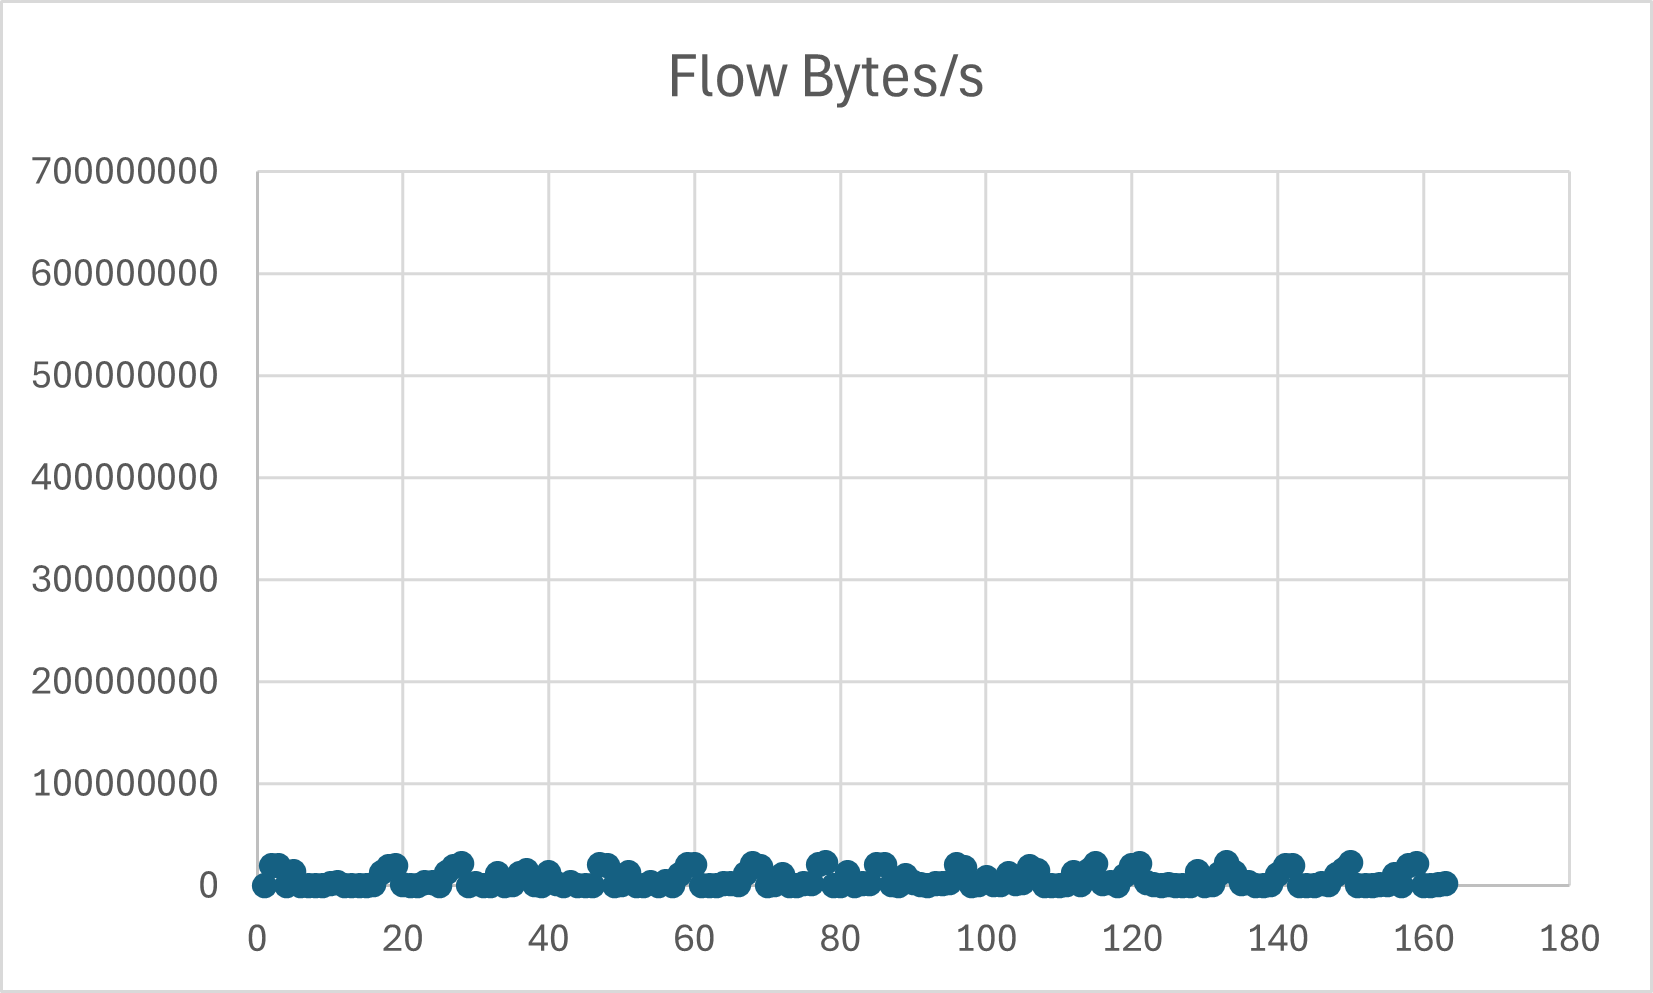
\includegraphics[width=\textwidth]{flow-bytes-attack}
      \caption{良性流}
    \end{subfigure}
    \bicaption{\enspace 流速散点图}{\enspace Scatterplot of Flow Rate}
    \label{fig:flow-bytes}
\end{figure}

此类特征同样难以区分横向移动流和良性流,因此难以直接用来识别横向移动。

因此,通过基于网络流量特征的最值检验,找出了横向移动中的 $5$ 个流,它们表示一个新建的 Pod 正在攻击者的控制下,向 API 服务器进行非法通信,进行恶意操作。然而,当这些流已经发生时才检测,往往为时已晚,最好在横向移动的更早阶段就能检测出来。因此,本节将基于机器学习进行网络流量特征筛选,为后续研究内容做好准备。

\subsection{基于网络拓扑结构的方法验证}

将网络流量的 IP 地址视为节点,节点之间的流量视为边,可以将网络流量以拓扑图的形式表现出来。数据集中良性流量的拓扑图如图~\ref{fig:benign-structure-ip}~所示。

\begin{figure}[!htbp]
    \centering
    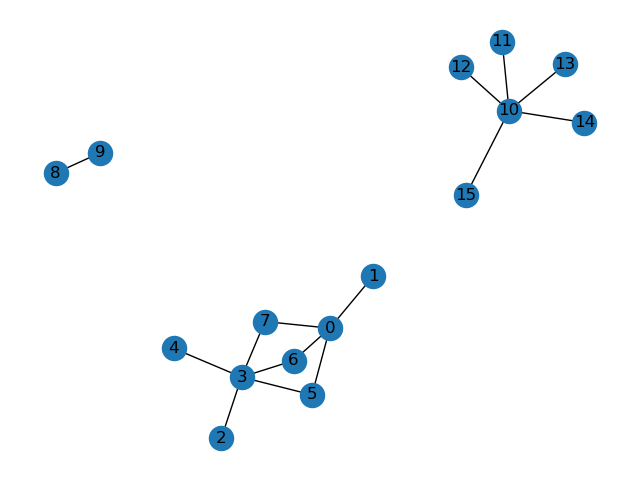
\includegraphics[width=0.75\textwidth]{benign-structure-ip}
    \bicaption{\enspace 良性流的网络拓扑结构}{\enspace Topological Diagram of Benign Flows}
    \label{fig:benign-structure-ip}

\end{figure}

包含良性流量和横向移动流量的拓扑图如图~\ref{fig:all-structure-ip}~所示。

\begin{figure}[!htbp]
    \centering
    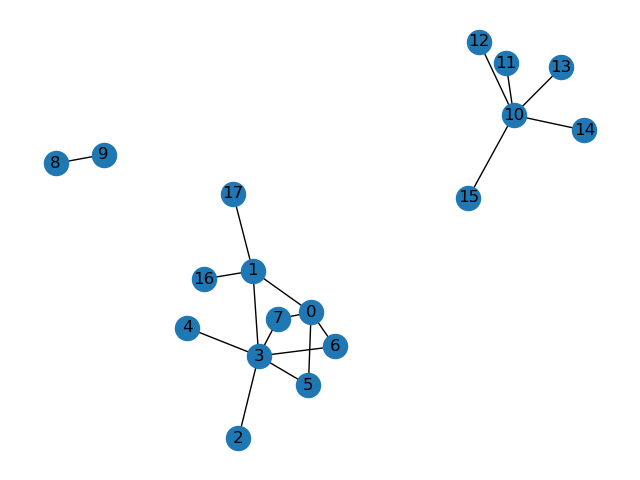
\includegraphics[width=0.75\textwidth]{all-structure-ip}
    \bicaption{\enspace 所有流的网络拓扑结构}{\enspace Topological Diagram of All Flows}
    \label{fig:all-structure-ip}

\end{figure}

图~\ref{fig:benign-structure-ip}~和图~\ref{fig:all-structure-ip}~中各节点所对应的 IP 地址如表~\ref{tab:cross-reference}~所示。

\begin{table}[!htbp]
    \bicaption{\enspace 节点与 IP 地址对照表}{\enspace Cross-reference Between Nodes and IP Addresses}
    \label{tab:cross-reference}
    \centering
    \footnotesize% fontsize
    \setlength{\tabcolsep}{4pt}% column separation
    \renewcommand{\arraystretch}{1.2}%row space 
    \begin{tabular}{cccccc}
        \hline
        编号 & IP 地址 & 备注\\
        \hline
        0 & 100.64.0.2 & 主机节点\\
        1 & 10.16.0.45 & 带有 Node-RED 软件的 Pod 节点\\
        2 & 10.16.0.2 & Pod 节点\\
        3 & 144.122.71.18 & API 服务器节点\\
        4 & 10.16.0.6 & Pod 节点\\
        5 & 10.16.0.5 & Pod 节点\\
        6 & 10.16.0.4 & Pod 节点\\
        7 & 10.16.0.7 & Pod 节点\\
        8 & 10.16.0.9 & Pod 节点\\
        9 & 18.165.61.116 & 外部节点\\
        10 & 10.16.0.18 & Pod 节点\\
        11 & 34.120.177.193 & 外部节点\\
        12 & 185.199.111.133 & 外部节点\\
        13 & 185.199.108.133 & 外部节点\\
        14 & 185.199.110.133 & 外部节点\\
        15 & 185.199.109.133 & 外部节点\\
        16 & 144.122.71.36 & 外部节点\\
        17 & 95.179.254.105 & 外部节点\\
        \hline
    \end{tabular}
\end{table}

通过图~\ref{fig:benign-structure-ip}~和图~\ref{fig:all-structure-ip}~的对比,可以看出,在正常情况下,节点 1 既不与外部节点通信,也不与 API 服务器通信。然而,当攻击者发起攻击后,节点 1 开始同时与外部节点和 API 服务器通信,这表明攻击者侵入 Node-RED 所在的 Pod 之后,操纵其向 API 服务器执行非法操作。因此,节点 1 与 API 服务器的通信和节点 1 与外部网络之间的通信均应发出警报,这对应 8 个流,具体如表~\ref{tab:dataset-topology-detect}~所示。

\begin{table}[!htbp]
    \bicaption{\enspace 基于网络拓扑结构的方法检出的横向移动流}{\enspace Malicious Flows Detected by Method Based on Topology}
    \label{tab:dataset-topology-detect}
    \centering
    \footnotesize% fontsize
    \setlength{\tabcolsep}{4pt}% column separation
    \renewcommand{\arraystretch}{1.2}%row space 
    \begin{tabular}{ccccccc}
        \hline
        源 IP 地址 & 源端口 & 目标 IP 地址 & 目标端口 & 能否被检测出?\\
        \hline
        144.122.71.36 & 9001 & 10.16.0.45 & 48754 & 是\\
        10.16.0.45 & 45956 & 144.122.71.18 & 6443 & 是\\
        10.16.0.45 & 46988 & 144.122.71.18 & 6443 & 是\\
        10.16.0.45 & 47002 & 144.122.71.18 & 6443 & 是\\
        10.16.0.45 & 52904 & 144.122.71.18 & 6443 & 是\\
        10.16.0.45 & 52906 & 144.122.71.18 & 6443 & 是\\
        10.16.0.45 & 54902 & 144.122.71.36 & 9001 & 是\\
        10.16.0.45 & 59624 & 95.179.254.105 & 443 & 是\\
        \hline
    \end{tabular}
\end{table}

\section{本章小结}

本章通过最值检测和拓扑分析的方式,将横向移动最关键阶段检测出来。在这个阶段,攻击者操控他所入侵的 Pod,与 API 服务器进行非法通信,以便进一步进行机密窃取、操控集群等行为。

然而,仅仅检测最关键阶段是不够的。如果在这个阶段才进行检测,往往为时已晚,因此我们需要在横向移动更早期的阶段就进行检测。这将在下一章中讨论。

}
% \chapter{网络流量空间和时间特征转换方法}{
{
\let\cleardoublepage\relax
}



}
% \chapter{原型系统设计}{
{
\let\cleardoublepage\relax
}

\section{系统整体架构设计}

系统整体架构如图~\ref{fig:system}~所示。

\begin{figure}[!htbp]
    \centering
    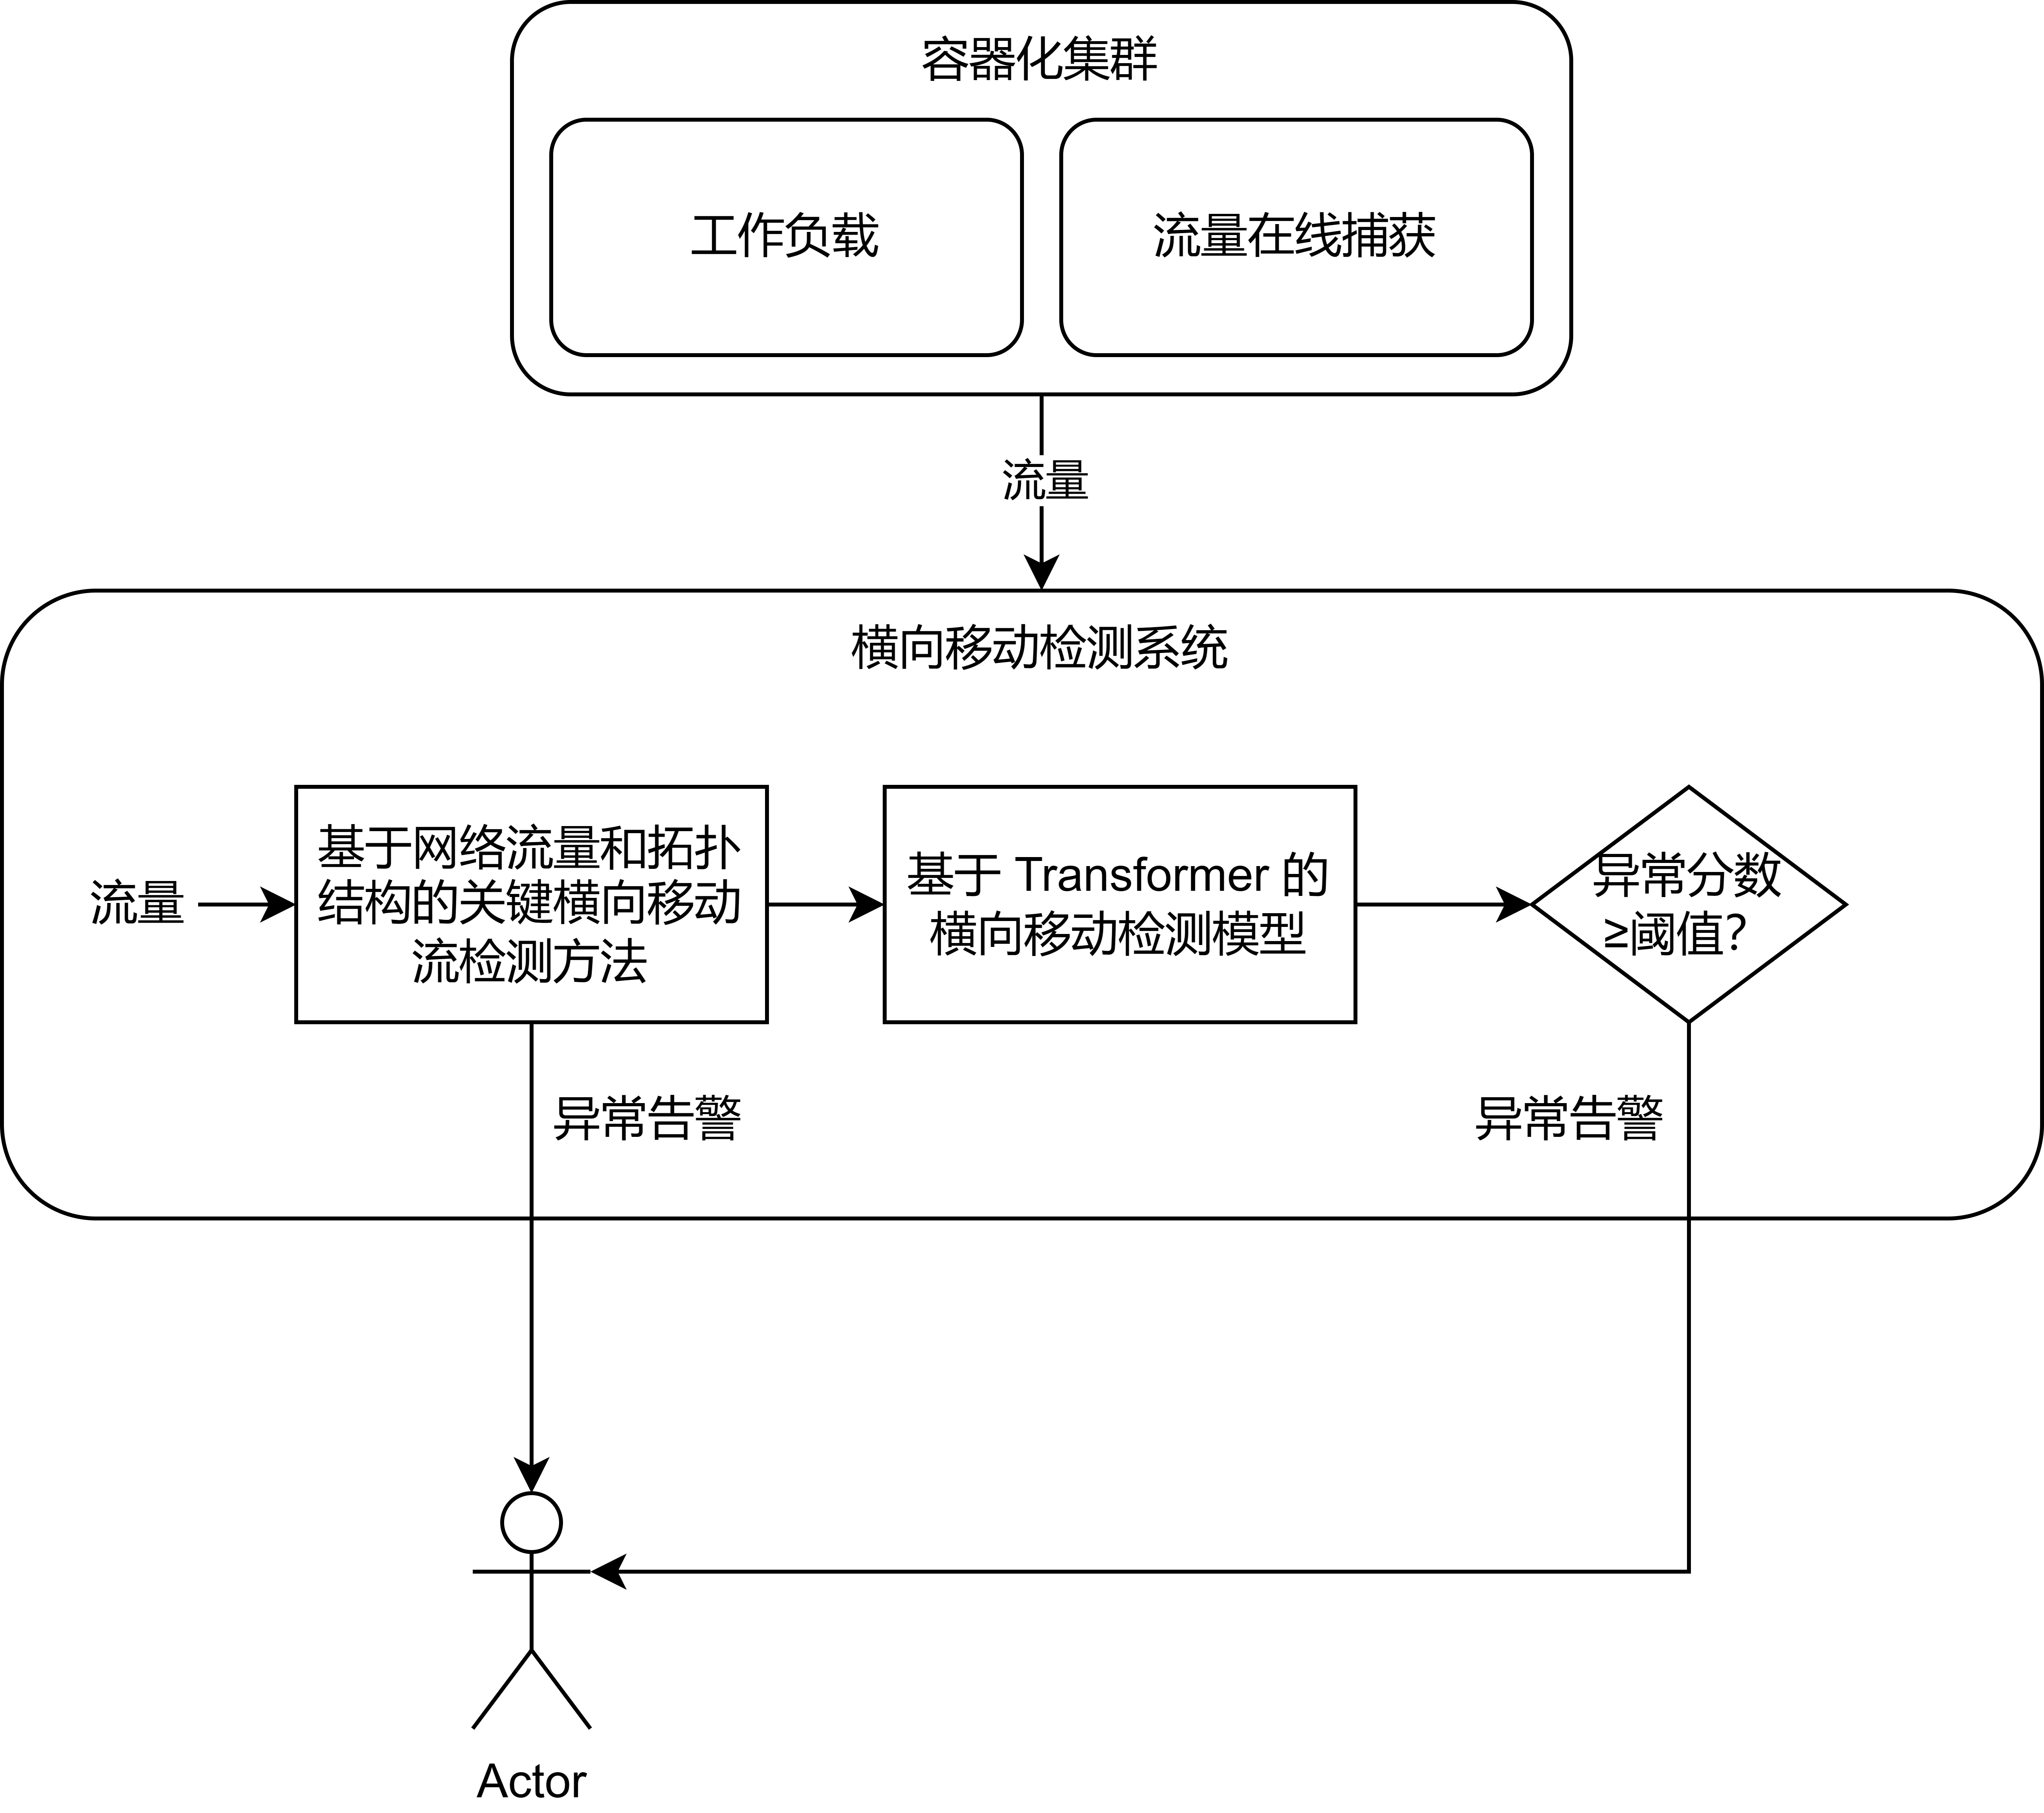
\includegraphics[width=1.00\textwidth]{system}
    \bicaption{\enspace 系统整体架构}{\enspace The System Architecture}
    \label{fig:system}

\end{figure}

主要分为三个模块:流量在线捕获模块、横向移动检测系统、告警模块,其中横向移动检测系统由基于网络流量和拓扑结构的关键横向移动流检测方法和基于 Transformer 的横向移动检测模型组成。

}
\chapter{引言}{
{
\let\cleardoublepage\relax
}

\section{研究背景与意义}

在现代的计算系统和软件工程领域,标准化和封装起非常重要的作用,它可以确保各项技术和工具在各种不同的底层技术上都能正常工作。容器就是这样的技术,它可以使应用程序在不同的底层操作系统上都能保持正常运行,使应用程序具有可移植性。容器的高度标准化催生了云原生技术,它使应用程序和容器的管理可以自动化实施,降低了维护系统的负担,减少了运营支出成本,并消除了开发人员与系统运营人员之间沟通的障碍\citep{cloudnative}。

因此,容器化的软件越来越广泛地得到采用。根据 Morder Intelligence 的报告\citep{mordor2024},应用程序容器市场规模预计将从2024年的54.5亿美元增长到2028年的194.1亿美元。根据 CNCF 组织发布的 2022 年度调查报告\citep{cncf2024},79\%的企业用户正在使用容器技术,其中有44个百分点的企业用户在绝大多数生产环境的应用中使用了容器。

然而,目前容器化环境正在遭受威胁。根据 Red Hat 的调查\citep{redhat2023sec},在全球 600 名大中小型企业的专业人员中,有 67\% 报告他们因容器化集群的安全问题而降低了部署速度,有 37\% 报告他们因容器安全事件而遭受经济损失。Aqua Security 的一次实验\citep{michael2024}发现有超过350个组织和个人的容器化集群不受保护,至少有60\%被攻击者利用,横跨金融、航空航天、汽车、工业、安全等领域。攻击者正在利用容器化集群来进行加密挖矿活动、收集机密、创建后门等。在 Docker Hub 上,用于挖掘门罗币(Monero)的矿工镜像已有超过100万次拉取。因此,提升容器化环境的安全性迫在眉睫。

容器化环境中的攻击通常分五个阶段进行,以便攻击者实现其目标\citep{alshamrani2019survey, armo2024}。这五个阶段如下:

\begin{enumerate}
    \item 侦察:攻击者探测他想要攻击的目标计算机或网络。在此阶段,他们可以获取各种信息,例如镜像、部署、Pod、节点和集群的状态等\citep{mitre2024}。
    \item 立足:攻击者成功进入目标计算机或网络。攻击者可以通过错误配置的集群组件、容器上存在的已知漏洞、零日漏洞、供应链植入、访问令牌窃取\citep{oshrat2024}等方式进入集群中。
    \item 横向移动:攻击者在目标网络内移动,在避免被检测系统发现的同时,搜索目标网络的更多内部信息,同时试图达到阶段性目标。攻击者可在此阶段获取集群的机密信息和访问令牌,创建新的具有特权的容器,访问内部资源,部署攻击脚本等。
    \item 攻击:在此阶段,攻击者达到他的最终目标,例如破坏网络中的关键组件,获取目标组织的内部数据,或者进行勒索等。
    \item 清理:攻击者在此阶段清除痕迹,以免被发现。
\end{enumerate}

在上述阶段中:

\begin{itemize}
    \item 若在侦察阶段进行检测,由于该阶段的攻击通常是被动进行的,被动攻击不会修改或干扰通信,而是监听或监视传输的信息\citep{app10113874},因此难以检测。具体来说,攻击者可能会在网络上查找公开的容器、公开的代码存储库\citep{oshrat2024}、应用程序的版本等等。
    \item 若在立足阶段进行检测,则需要了解攻击者进入集群的途径。攻击者可能通过接入方式或漏洞利用的方法进入集群中\citep{7550947}。通过接入的方式进入集群时,攻击者利用在侦察阶段找到的公开的容器进入集群;或者利用公开的代码存储库,通过供应链攻击进入集群\citep{cicd}。通过漏洞利用的方法进入集群时,攻击者通过使用较旧版本的软件或零日漏洞进入集群中\citep{7550947}。因此,在该阶段进行检测和防御,需要综合使用多种手段,这超出了本文的范围。
    \item 若在攻击、清理阶段进行检测,则攻击者已达到其目标,通常为时已晚。
\end{itemize}

本文关注在横向移动阶段的检测。当立足阶段的检测和防御措施失效时,及时地检测横向移动有助于阻止攻击者进一步破坏集群,防止危害扩大。攻击者进行横向移动的方式多种多样,Microsoft 提出的威胁矩阵\citep{yossi2020threat}总结了多达 45 种技术可用于攻击容器化集群。不过,可以留意到,攻击者在容器化集群内移动时,是通过网络的方式进行移动的。因此,本文将利用网络流量数据,检测容器化环境中的横向移动行为。

\section{挑战}

容器化环境中的横向移动检测任务的挑战如下:

\begin{itemize}
    \item {容器化集群可用于检测的特征不明确。
    
    现有的横向移动检测研究通常在企业网络等非容器化环境中进行,主要针对登录记录进行研究。这些登录记录包含了源计算机、目的计算机和登录用户信息。攻击者通常通过社会工程学或 Mimikatz\citep{mimikatz} 等工具窃取内网中其他账号的登录凭据,以便移动到其他计算机上,因此便留下了相应的登录记录信息。然而,在容器化集群中,攻击者进行横向移动的手段有所不同,他们进入系统后,使用容器内的环境变量、服务账户等凭据,或利用逃逸漏洞,以便移动到其他容器或主机上\citep{oshrat2024}。因此,容器化环境中不包含可用于横向移动检测的登录信息等特征,还需要进一步发掘可用于检测的特征。
    }
    \item {横向移动检测任务的分类难度大,且样本不均衡,对高检测率和低误报率提出了高要求。

    对于横向移动,攻击者会尽可能隐藏其行为,使其难以从正常行为中区分出来。此外,大部分流量均为正常流量,仅有极少数流量为横向移动流量,因此,在检测横向移动时容易导致警报泛滥问题,过多警报容易让人变得麻木,反而导致横向移动检测没有起到应有的效果。因此,横向移动检测任务需在较低误报率的情况下,尽可能提高横向移动的检测率。
    }
\end{itemize}

\section{主要研究内容}

为了应对上述挑战,本文将进行以下研究:

\begin{itemize}
    \item 针对容器化集群可用于检测的特征不明确的问题,本文从两个方面着手分析。在网络流量特征方面,本文首先将分析横向移动的原理及其在网络流量中的表现,进行网络流量中的特征分析,并对各特征进行重要度评估。特征分析和特征重要度评估的结果将在后续模型中使用。
    \item 在网络流量的时空特性方面,本文进行了拓扑分析和特征嵌入方法研究。本文从流量的空间和时间两方面进行了研究。在流量的空间方面,本文首先将进行流量的拓扑结构分析,明确各网络流量所起的作用并进行分类;然后,本文将研究基于图机器学习的空间特征嵌入方法,为流量的每个节点生成嵌入向量。在流量的时间方面,本文将研究基于循环神经网络的时间特征嵌入方法,为流量序列生成时间嵌入向量。拓扑分析的结果和嵌入向量将在后续模型中使用。
    \item 针对横向移动检测任务的检测性能问题,本文首先利用了特征分析和拓扑分析的结果,对于少数关键的横向移动检测行为进行检测;对于大多数横向移动流量,本文将提出基于深度学习的横向移动检测模型 LMDCE,该模型由空间特征嵌入模块、时间特征嵌入模块、编码器—解码器模块和两步预测机制构成。通过该模型,本文提出的方法达到了 96.401\% 的 AUC 分数,超过了现有其他横向移动检测模型在容器化环境下的表现。
\end{itemize}

本文的研究框架如图~\ref{fig:research}~所示。

\begin{figure}[t]
    \centering
    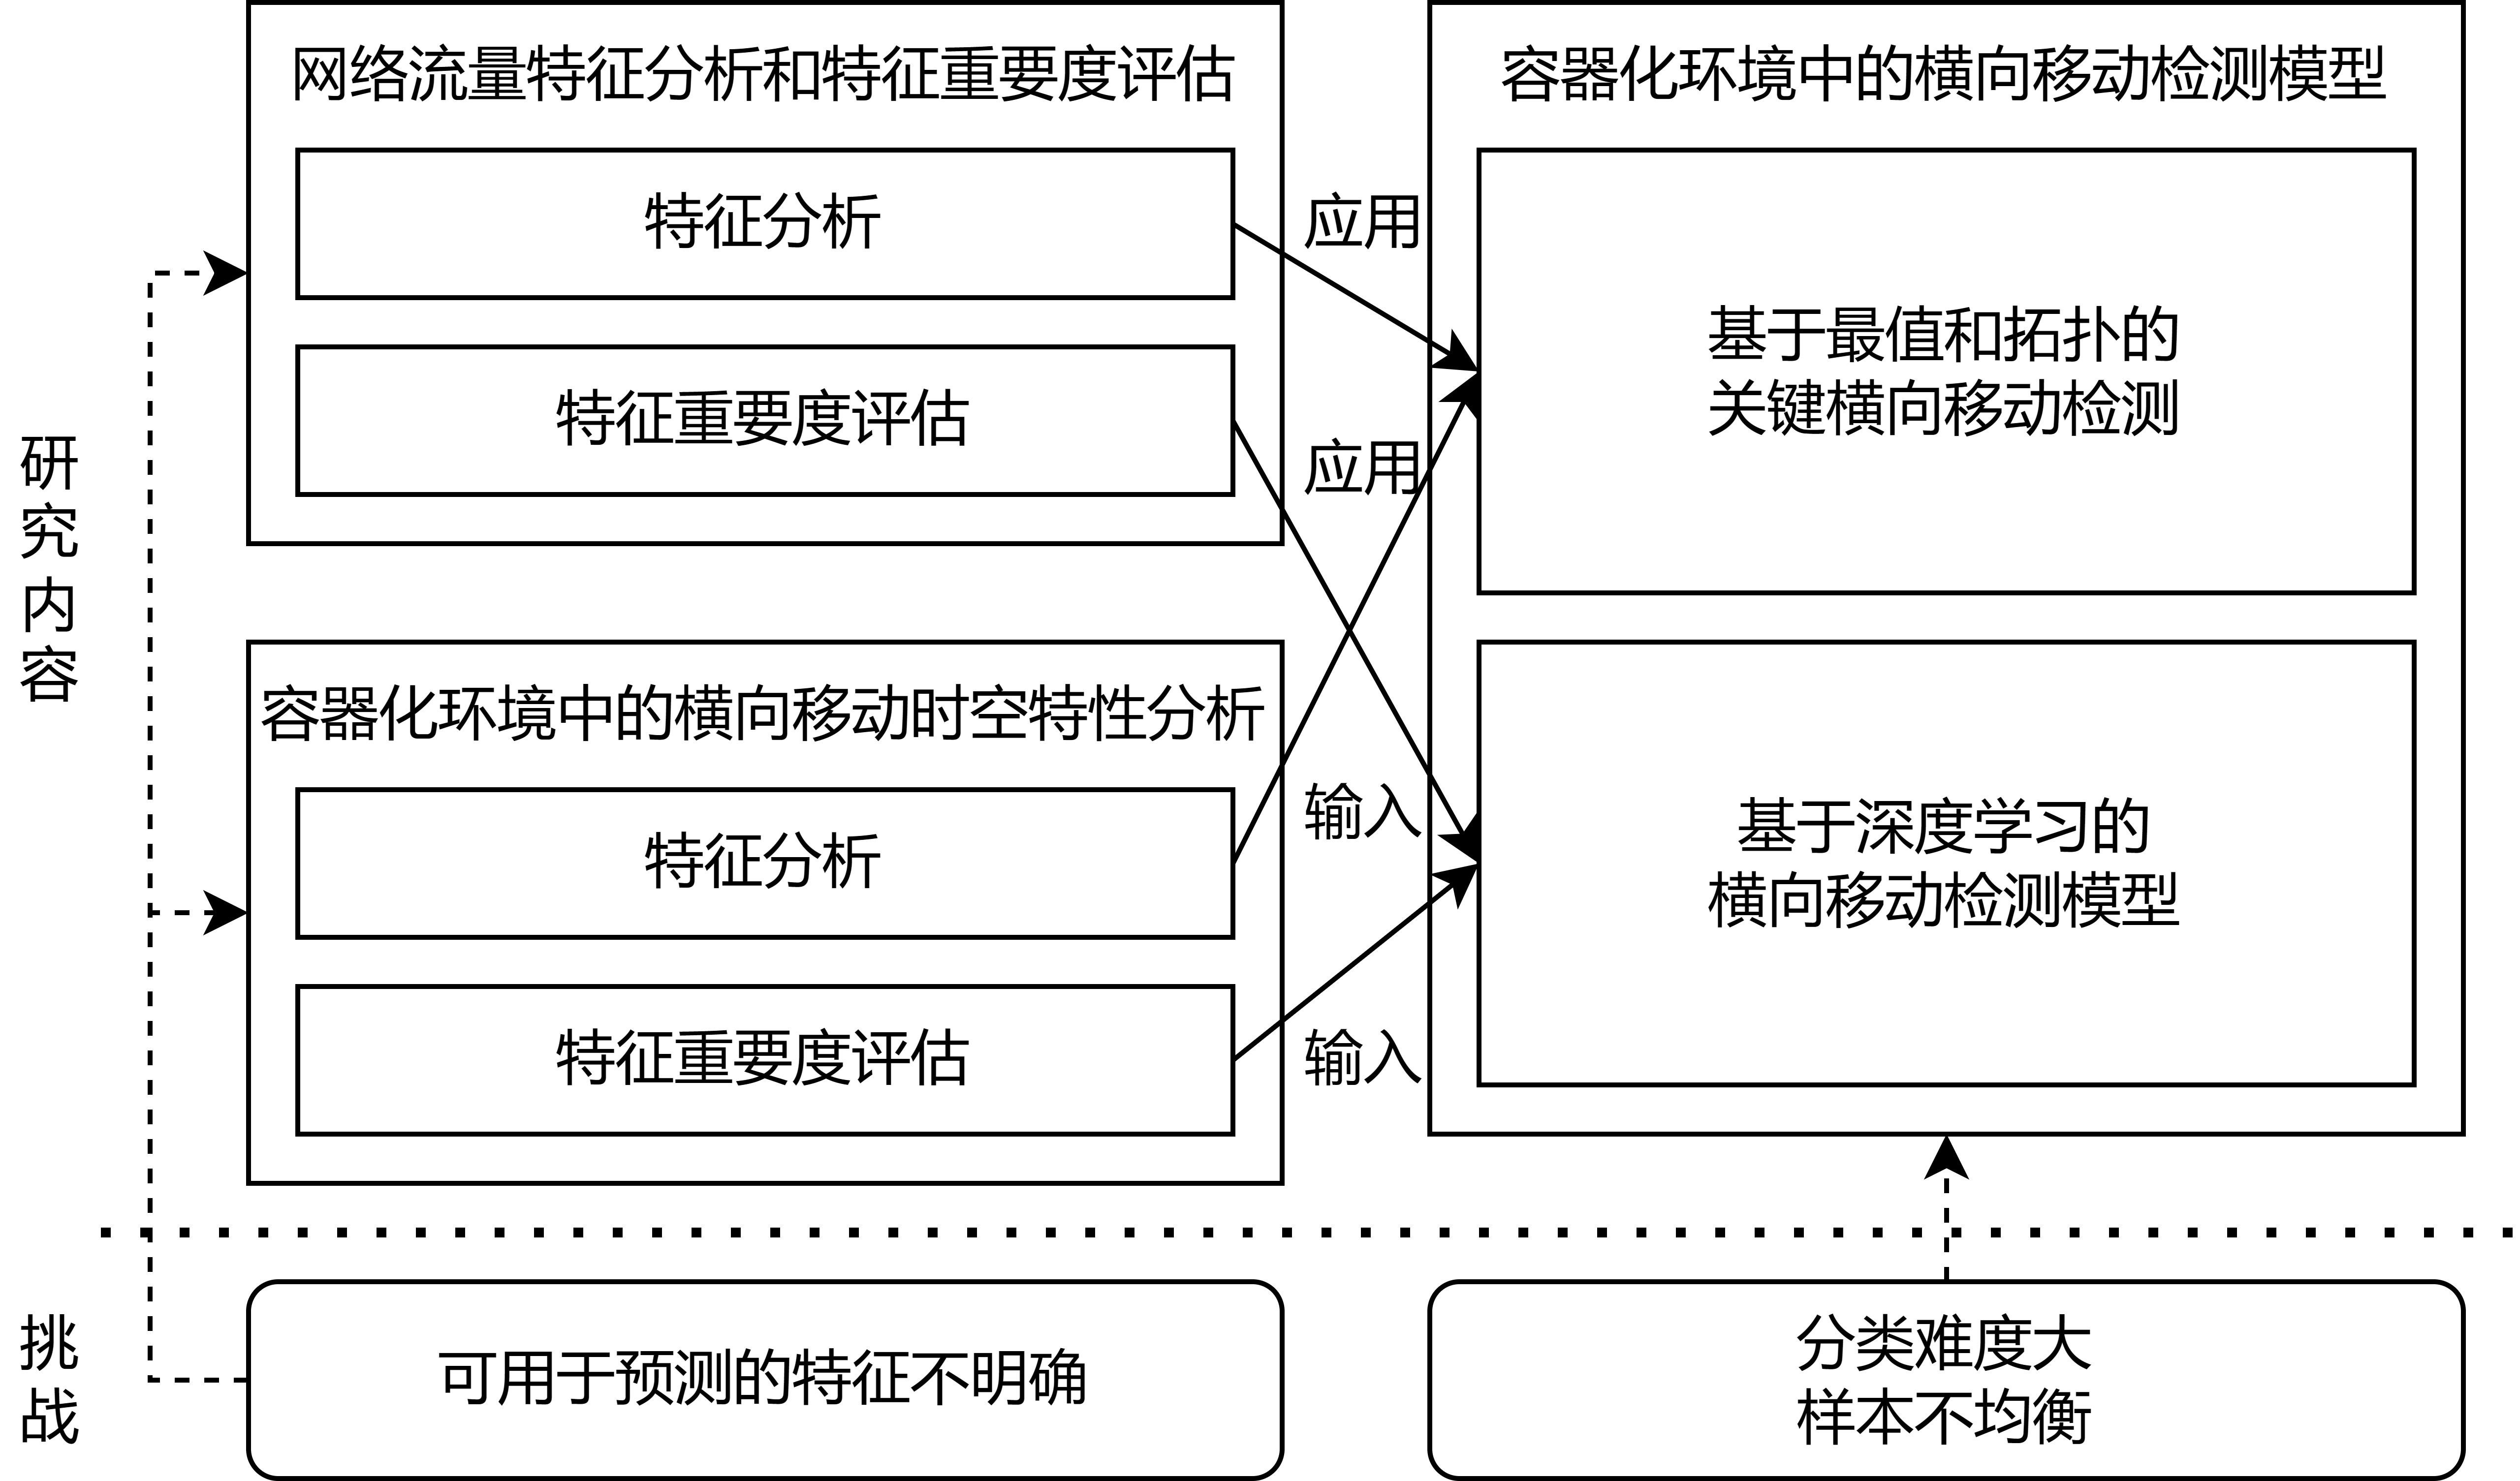
\includegraphics[width=0.8\textwidth]{research}
    \bicaption{\enspace 本文的研究框架}{\enspace The research framework of this thesis}
    \label{fig:research}
\end{figure}

\section{本文组织结构}

本文共分为六章,每章内容如下:

\begin{enumerate}
    \item 第一章:引言。该部分首先介绍了容器化环境中的横向移动检测的研究背景与意义,然后介绍了研究挑战及其对应的研究内容,最后介绍了本文组织结构。
    \item 第二章:相关研究成果与进展。该部分首先介绍了容器化环境及在该环境下存在的安全问题,然后分类介绍了现有的横向移动检测方法,指出这些方法均在非容器胡环境下应用,不能直接应用于容器化环境。接着,本文介绍了容器化环境中可行的横向移动检测技术路线。最后,介绍了本文所采用的数据集。
    \item 第三章:网络流量特征分析和特征重要度评估。首先,本文分析了容器化集群中横向移动的原理,接着通过最值分析,找到了最能体现关键的少数横向移动流量的特征,这些特征体现了横向移动导致数据传输量的变化。对于其余大部分横向移动流量,本文进行了密度分析,并采用机器学习算法进行了特征重要度评估,得到了按评估分数排列的特征列表。
    \item 第四章:容器化环境中的横向移动时空特性分析。首先,本文进行了网络流量的拓扑结构分析,指出在数据集所提供的横向移动场景中,最能体现横向移动的流量是从未与 API 服务器通信的容器开始与 API 服务器通信,同时与外部网络保持连接。接着,本文进行了空间和时间特征嵌入方法研究,分别得到了空间和时间特征嵌入向量,这些嵌入向量将作为后续检测模型的输入。
    \item 第五章:基于 Transformer 的两阶段横向移动检测方法。在第一阶段,本章首先利用了特征分析和拓扑分析的结果,提出了关键横向移动流量的检测方法。然后,在第二阶段,本章提出了一种基于 Transformer 的横向移动检测模型 LMDCE。最后,本章进行了实验,对方法和模型的各项性能进行对比验证。
    \item 第六章:总结与展望。对本文工作进行了总结,并分析了将来的研究方向。
\end{enumerate}
}
\chapter{研究背景和现状}{
{
\let\cleardoublepage\relax
}

\section{研究背景}

\subsection{容器化环境简介}

容器是应用程序的标准单元,它将应用程序的代码及其所有依赖项打包在内,以便在不同的硬件和软件环境中都可以正确执行,解决了兼容性问题,实现应用程序的可移植性\citep{whatcontainer}。相比起虚拟机,容器无需包含整个操作系统,因此容器是轻量化的,开销低\citep{Schenker2023}。由于不包含操作系统,因此容器需共享主机上的操作系统内核,这基于资源隔离技术实现\citep{Jain2020}。这些资源隔离技术包括:

\begin{itemize}
    \item 命名空间机制。将容器的网络、文件系统挂载、用户组等资源与主机隔离,使容器不能看到主机上的资源,而只能看到容器内部的资源。
    \item 更改根目录机制。将容器内的根目录限制在容器内部,避免容器读、写或执行主机上的文件。
    \item 控制组(Control Group,cgroup)机制。限制了容器可使用主机上的处理器、内存等资源的配额。
\end{itemize}

为了提高应用程序的可用性和稳定性,通常采用分布式体系结构。对于容器化的应用程序而言,则相应地采用分布式的容器化结构,这些运行不同容器的主机构成容器化集群。为了支撑容器化集群的管理,需要容器编排工具以提供资源配额、调度、负载均衡、运行状况检查、容错、自动缩放、自动修复等功能。

图~\ref{fig:orchestration}~展示了一个部署在云上的容器化集群的分层架构\citep{Casalicchio2019}。

\begin{figure}[t]
    \centering
    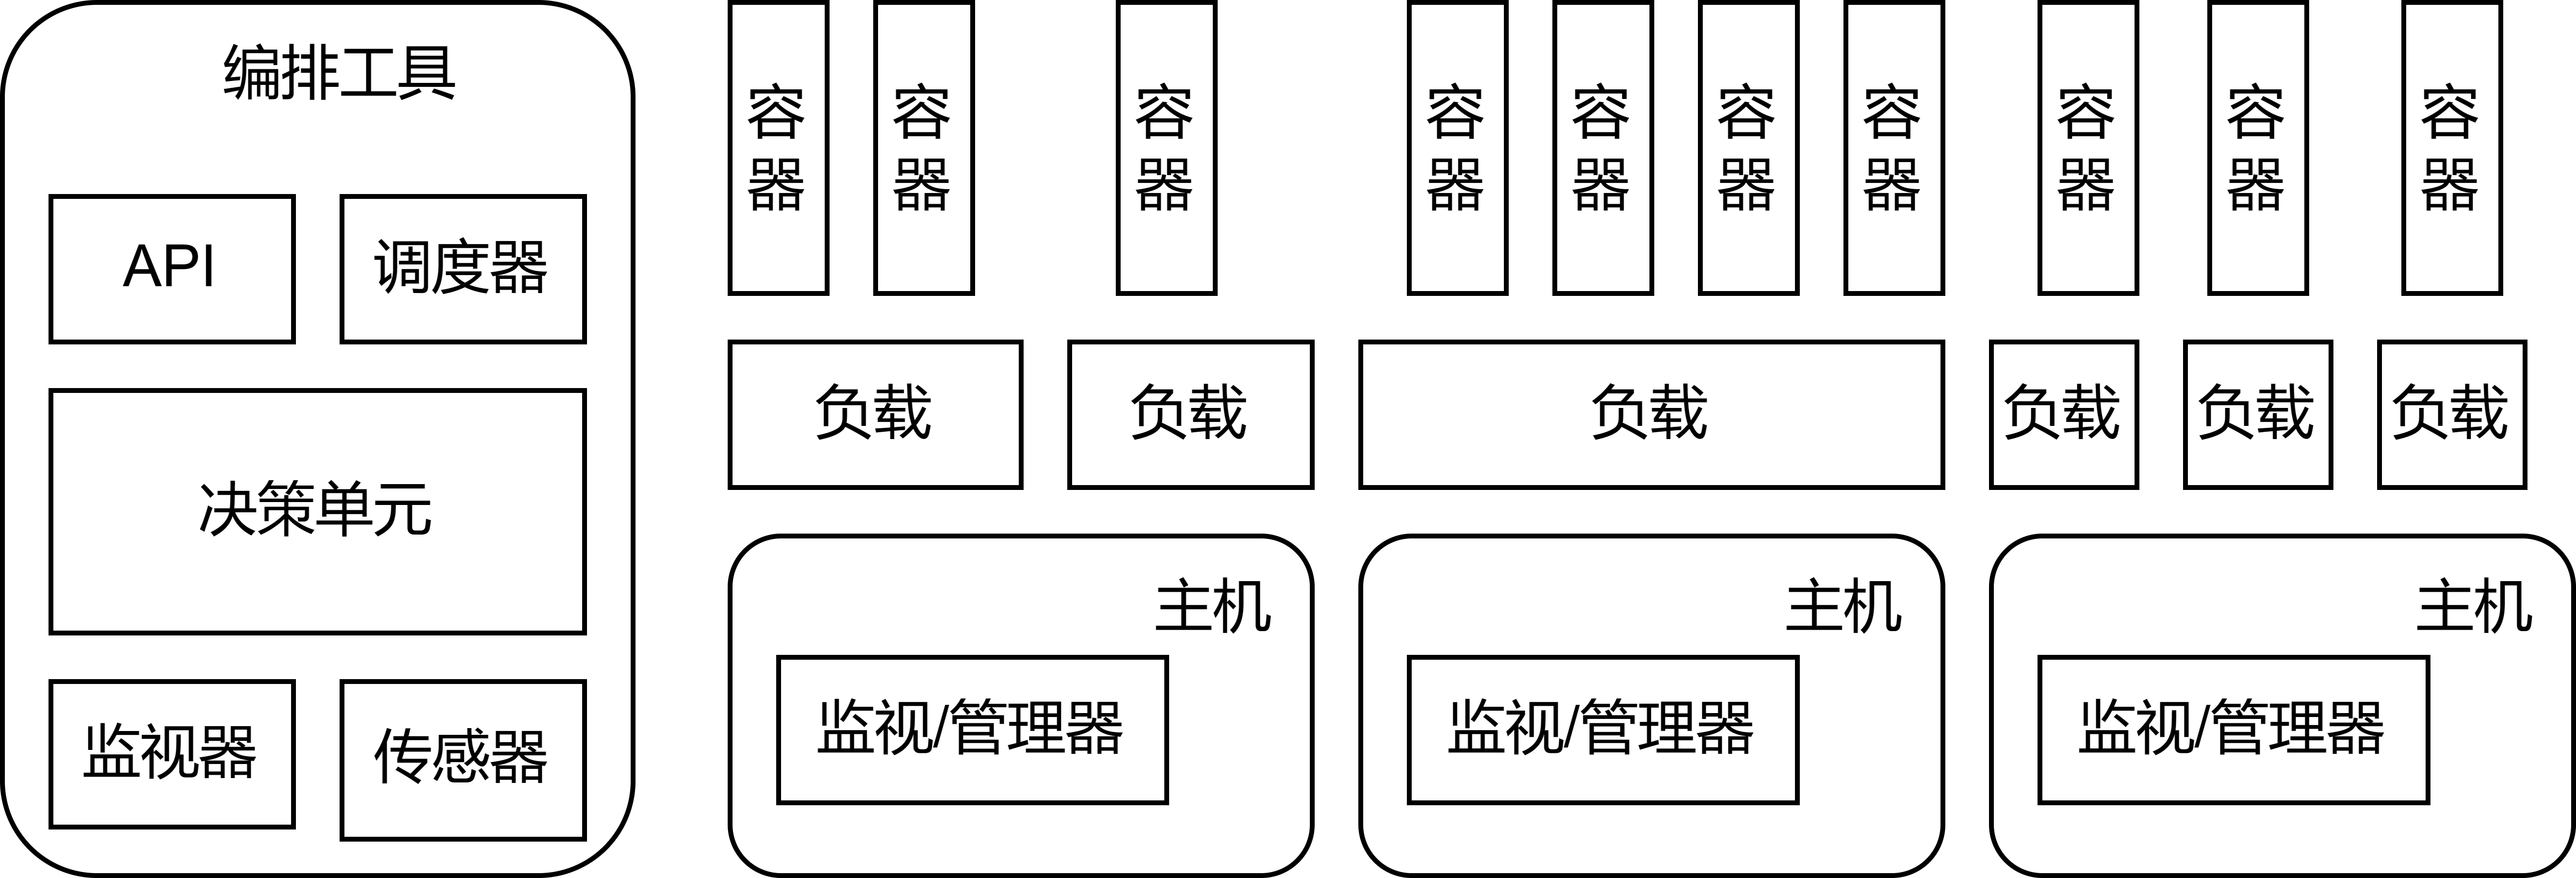
\includegraphics[width=1.00\textwidth]{orchestration}
    \bicaption{\enspace 容器化集群的架构}{\enspace The architecture of a containerized cluster}
    \label{fig:orchestration}

\end{figure}

容器化集群中的调度通常以负载为单位进行,单个负载中包含一个或多个容器,由编排工具的调度器调度到主机上。主机上均部署了监视器,将该主机的运行情况传输至编排工具的传感器中,以便编排工具检查主机的运行情况和工作载荷等。编排工具上也部署了监视器,负责检查负载及其包含的容器的运行状况(通常通过网络请求等方式探测)。编排工具的决策单元将根据用户设定的规则,执行自动缩放、自动修复等任务,具体任务通过主机上的管理器实施。编排工具还提供应用程序接口(Application Programming Interface,API),以便调整配置和管理集群中的资源。

\subsection{容器化环境下的安全问题}

由于容器化环境中包含多种多样的组件,因此其攻击面十分广泛,任何一个组件存在缺陷都会对容器化环境造成威胁。这些攻击面如图~\ref{fig:attack-vector}~所示\citep{liz2018}。

\begin{figure}[t]
    \centering
    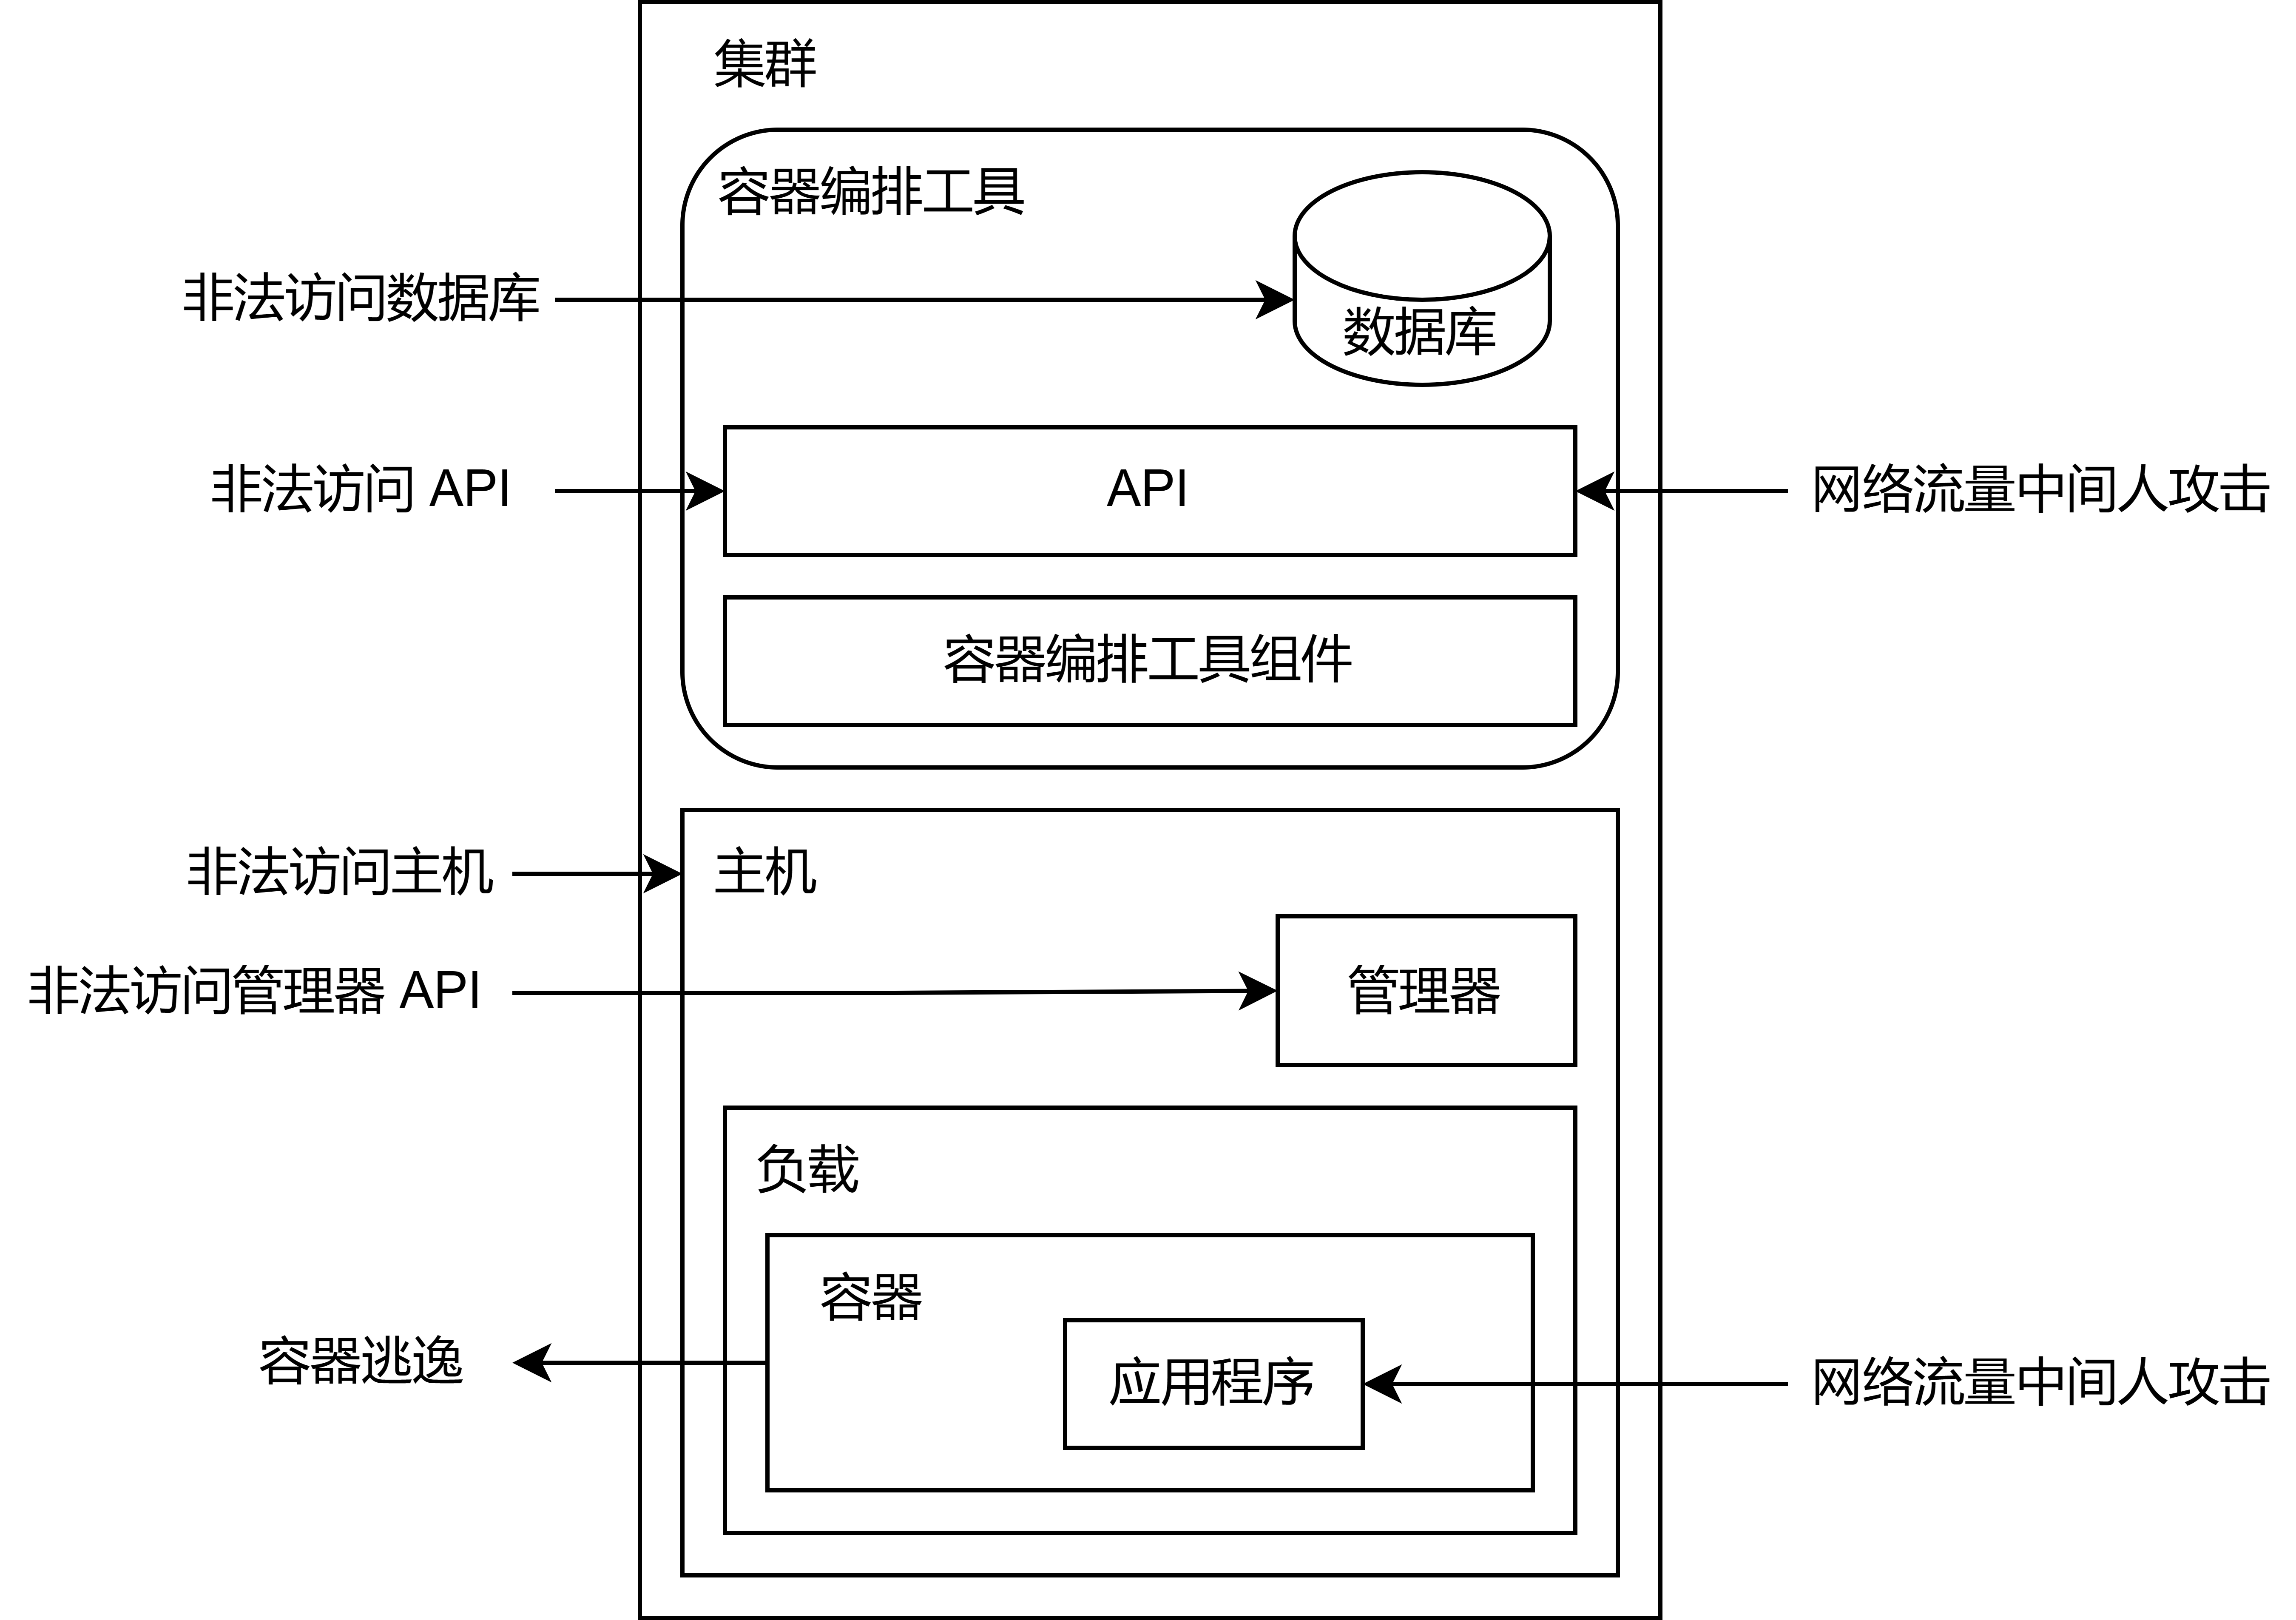
\includegraphics[width=1.00\textwidth]{attack-vector}
    \bicaption{\enspace 容器化集群的攻击面\citep{liz2018}}{\enspace Attack vectors of containerized clusters\citep{liz2018}}
    \label{fig:attack-vector}

\end{figure}

这些攻击面与 OWASP 基金会公布的网络应用程序十大安全风险\citep{owasp}相吻合。这些安全风险包括\citep{liz2020}:

\begin{itemize}
    \item 访问控制配置不当。由于容器通常在 Linux 操作系统上运行,而只有根用户才能使用资源隔离技术,所以容器默认情况下在根用户下运行,这就导致可能产生容器逃逸的风险。此外,在容器化集群中,访问控制配置不当还会产生 API 被滥用,导致数据泄露或系统无法正常运行的风险。
    \item 加密信息泄露。虽然容器编排工具的 API 默认仅允许加密流量,但开发者仍需自行为应用程序的流量加密负责。若进行了明文传输,则会导致应用程序存在被攻击的风险,从而使容器化集群陷入威胁。
    \item 注入漏洞。注入漏洞可能存在于各种 API 请求中,因此容器编排工具、主机上的管理器和应用程序都面临风险。
    \item 不安全的设计。若容器化集群未经过最小特权原则、纵深防御原则、零信任原则和安全开放原则设计,则会面临威胁。
    \item 安全配置错误。在容器化集群中,使用环境变量传递密钥会导致这些密钥通过日志泄露,威胁集群的安全。
    \item 易受攻击和过时的组件。若容器使用过时的应用程序版本,则该容器可能会包含漏洞,导致攻击者入侵到容器中。
    \item 身份认证失败。攻击者通过撞库、弱密码、盗窃会话标识符等方式登录到应用程序中,使容器化集群面临风险。
    \item 软件和数据完整性丢失。攻击者通过污染公开的应用程序源发起供应链攻击,当集群中的容器使用这类应用程序时,导致集群面临威胁。
    \item 不充分的监控和日志。平均而言,违规行为需要近 200 天才能被识别\citep{liz2020}。通过详细记录网络入站和出站等容器事件,可以显著减少这种情况。
    \item 服务器端请求伪造。这会面临内部的端口扫描、元数据和敏感数据泄露、内部服务被破坏等威胁。
\end{itemize}

因此,通过充分地监控并记录网络连接日志,可以减少容器化环境中存在的威胁。本研究基于网络流量展开横向移动检测的研究。

\section{现有横向移动检测方法}

为检测横向移动,可运用多种技术和方法。通常,可以从网络流量、端点行为、用户行为和威胁情报四方面进行检测:

\begin{itemize}
    \item 基于网络流量的检测:可通过异常的端口扫描、大量的数据传输、使用非标准协议的通信等方面进行检测;
    \item 基于端点行为的检测:可通过异常的进程创建、异常的文件访问、异常的注册表修改等方面进行检测;
    \item 基于用户行为的检测:可通过登录异常账户、访问异常的资源、执行异常的操作等方面进行检测;
    \item 基于威胁情报的检测:攻击者通常会使用已知的工具和技术进行横向移动。通过分析威胁情报,可以识别出攻击者可能使用的工具和技术,并提前进行防御。
\end{itemize}

\subsection{基于端点行为和威胁情报的检测}

Latte\citep{liu2018latte} 利用 Windows 系统和安全事件构建网络连接图,当网络中发生远程文件执行(常规检测场景)或者检测到被攻击的节点(取证分析场景)时,可利用该网络连接图找到可能的横向移动路径。然而,该方法与 Windows 系统深度绑定,无法用于容器化环境中的检测。

\subsection{基于用户行为的检测}

Log2vec\citep{liu2019log2vec}通过对用户操作日志(如登录、访问网页、发送邮件、打开文件等)建模成图,生成各节点的嵌入向量后,通过一种聚类方法,将较小的聚类认定为异常操作。在容器化场景中,没有用户行为的信息可以利用,TCP/IP 流量中也无相关用户行为信息。不过,在容器化集群中,各 Pod 的日志或许可用于横向移动检测,这有待未来的工作。

\subsection{基于网络流量的检测}

大多数横向移动检测方法通过网络流量来检测横向移动,但它们仅关注由登录活动产生的网络流量。这方法基于一个关键的假设:攻击者通常执行横向移动来访问最初的受害者无法访问的机器。

这些方法检测横向移动的模型各不相同,但都采取了将网络流量日志建模成登录图的方法,其中图的节点代表计算机,边代表计算机之间产生的流量。这些方法如表~\ref{tab:recent}~所示。

\begin{table}[t]
    \bicaption{\enspace 现有横向移动检测方法}{\enspace Recent lateral movement detection methods}
    \label{tab:recent}
    \centering
    \footnotesize% fontsize
    \setlength{\tabcolsep}{4pt}% column separation
    \renewcommand{\arraystretch}{1.2}%row space 
    \begin{tabular}{ccccccccc}
        \hline
        方法 & 机器学习模型 & 数据集 & 效果\\
        \hline
        Kent 等人\citep{kent2015authentication} & 无 & LANL\citep{kent-2015-cyberdata1} & 检测率28\% 误报率0.13\%\\
        Siadati 等人\citep{siadati2017detecting} & 无 & 私有数据集 & 检测率82\% 误报率0.3\%\\
        Bowman 等人\citep{bowman2020detecting} & Node2vec\citep{grover2016node2vec}、Logistic & LANL\citep{kent-2015-cyberdata1} & 检测率85\% 误报率0.9\%\\
        Hopper\citep{ho2021hopper} & 无 & 私有数据集 & 检测率94.5\% 误报率0.12\%\\
        Euler\citep{king2023euler} & GCN\citep{kipf2016semi}、GRU\citep{cho2014learning} & LANL\citep{kent-2015-cyberdata1} & 检测率86.1\% 误报率0.57\% AUC 99.12\%\\
        Jbeil\citep{khoury2023jbeil} & TGN\citep{rossi2020temporal} & LANL\citep{kent-2015-cyberdata1} & AUC 99.31\%\\
        \hline
    \end{tabular}
\end{table}

可以看到,这些方法采用的数据集及其评估指标不尽相同,并且均在企业网络等非容器化环境下进行横向移动检测,未对容器化场景进行研究。

Kent 等人\citep{kent2015authentication}通过提取图的特征后,使用 Logistic 回归模型检测横向移动。该方法提取图的特征包括图的节点数、边数、图形密度等。这种提取方法在图神经网络流行的今天看起来已经十分老旧,实现起来比较繁琐,并且效果欠佳。

Siadati 等人\citep{siadati2017detecting}统计挖掘了若干个最常通信的用户、源计算机、目标计算机三元组$\left<U,S,D\right>$,对于一个登录记录$\left<u,s,d\right>$,若该登录记录符合其中一个三元组即$u \in U, s \in S, d \in D$,则认为该登录是正常的;否则认定为横向移动。该方法的优点是可解释性强;缺点是其三元组的挖掘方式较低效,需要枚举所有可能的 $\left<U,S,D\right>$,用时较长。

Bowman 等人\citep{bowman2020detecting}是首个采用了机器学习的方法,它采用 Node2vec 模型学习登录图并生成各节点的嵌入向量,对于每条登录记录,计算该登录记录中两个节点的逐元素乘积并通过 Logistic 模型预测该登录记录为横向移动的概率。该方法的优点是采用了机器学习的方法,比先前的方法更有效地提取图的特征;缺点是它将登录图视为静态的,未能体现网络的动态性,对于原本正常但后来被感染的计算机,难以检出其横向移动行为。

Hopper\citep{ho2021hopper}则对路径之间的因果关系进行了深入研究。该方法定义了登录记录之间因果关系的聚合方法,对于两条登录记录 $L_1=\left<s_1, d_1\right>$ 和 $L_2=\left<s_2, d_2\right>$,若 $L_1$ 发生在 $L_2$ 之前 24 小时之内,并且 $L_1$ 的目的计算机等于 $L_2$ 的源计算机即 $d_1=s_2$,那么 $L_1$ 与 $L_2$ 呈``因果关系'',$L_1$ 是 $L_2$ 的原因。多条因果登录记录通过上述规则聚合为登录路径。Hopper 检查登录路径上的用户信息,若用户信息发生了变化,则视为横向移动;若用户信息没有发生变化,则不是横向移动。然而,由于因果关系聚合方法不够精确,一条登录记录的原因可能是多条登录记录之一而无法准确判断,对于这类不明确且可能存在用户信息变化的登录路径,Hopper 通过历史登录记录和历史告警记录推断发生横向移动的概率。该方法的优点是考虑了登录路径的时序关系,缺点是其登录路径规则聚合方法较繁琐,且需排除多种白名单情况(例如跳板机、新机器等),导致其准确率还有待提高。此外,该方法在私有的 Dropbox 数据集上完成,其检测结果无法与其他方法直接对比。

Euler\citep{king2023euler}采用类似 GCRN\citep{seo2018gcrn} 模型的方式将图深度学习网络和循环神经网络堆叠起来。该方法首先根据设定的时间间隔,划分时间片,为每个时间片生成一张登录图;然后,使用图深度学习网络为登录图中每个节点生成嵌入向量;接着将这些向量输入到循环神经网络中,得到下一时刻节点嵌入向量的预测;再对两个节点的嵌入向量进行点积,就得到这两个节点存在登录记录的概率,将概率较低者判定为横向移动。图深度学习网络为 GCN、GraphSAGE\citep{hamilton2017inductive}、GAT\citep{velivckovic2017graph} 任选其一,循环神经网络为 GRU、LSTM\citep{hochreiter1997long}、None(即使用恒等映射)任选其一。该方法的优点是考虑了网络的动态性,并结合了深度学习方法,使其准确性大大提高;缺点是需要划分时间片,使每个时间片内部的时序关系丢失。

Jbeil\citep{khoury2023jbeil}是企业网络内检测横向移动的最新方法。它引用 TGN 模型,避免了时间片的划分。该方法由图特征提取模块、记忆模块和嵌入模块两方面构成。对于图特征提取模块,模型计算每个节点每日的特征,例如该节点当日用户登录数、节点当日登录计算机数等。对于节点的记忆模块,模型按时间顺序处理每条登录记录,更新登录记录源节点和目的节点的记忆向量,节点记忆向量的更新采用循环神经网络。对于节点的嵌入模块,模型枚举节点的每一个历史邻居节点,将节点当时的记忆向量、节点当时的特征、历史邻居节点当时的记忆向量、历史邻居节点当时的特征通过注意力函数得到节点当前的嵌入向量。最后,模型将两个节点的嵌入向量经过解码器,得到这两个节点存在边的概率,将概率较低者判定为横向移动。该方法的优点是无需划分时间片,因此不会丢失时间数据,这使得其准确率大大提高。

上述方法的共同缺点在于,它们均采用了图的链路预测方式来检测横向移动,即判断两个节点存在登录记录的概率。然而,在容器化场景中,没有相应的登录记录信息可用,因为攻击者入侵到集群中时并非是根据任何人的身份信息登录到集群中,而是利用负载的漏洞等,通过远程代码执行的方式入侵到集群中。此外,容器化集群的 API 服务器虽然负责进行身份认证和鉴权,但涉及集群内部操作时,API 服务器主要鉴定的是负载、主机的身份,而非人的身份。

在容器化集群中,使用网络流量信息来检测横向移动时,也不能简单地采用图的链路预测方法。因为这类方法仅判断边的存在性,而没有考虑边上的特征;但在容器化集群中,边上的特征即网络流量的特征发挥非常重要的作用。这将在第~\ref{sec:analyze}~节中详细描述。

\section{容器化环境中的横向移动检测技术路线}

横向移动是网络入侵攻击的一个阶段,因此横向移动检测是入侵检测系统的一类。基于网络流量的入侵检测系统通常有如下可行的技术路线\citep{ahmad2021network, darban2022deep}:

\begin{itemize}
    \item 传统机器学习方法。包括决策树、K-最近邻、K-均值、支持向量机等。这些方法实现简单,运行速度快,但准确率低。
    \item 循环神经网络方法。循环神经网络用于预测一个序列在下一个时刻的值,当预测值与实际值误差较大时,判定为攻击。循环神经网络的变体包括 GRU、LSTM 等,解决梯度消失导致模型无法捕获长距离依赖关系的问题。此外,基于自注意力机制的 Transformer\citep{vaswani2017attention} 模型也可用于取代循环神经网络,因为 Transformer 可并行处理序列,同时仍然保持模型的性能。
    \item 自动编码器。自动编码器由编码器和解码器构成,编码器将输入压缩为隐向量,解码器则将隐向量还原至原来的维度,试图重现原来的输入,然后再重现值与输入对比,误差较大者视为攻击。
    \item 生成对抗网络。生成对抗网络中通常包含生成器和判别器,生成器用于生成与输入尽可能相似的样本,判别器用于尽可能准确地将生成器生成的样本与输入区分开来。通过这种对抗训练方法,可以提高生成器重现输入样本和判别器判断异常样本的准确性。
\end{itemize}

近年来,有许多工作关注上述这几种技术路线。

USAD\citep{audibert2020usad} 使用两个自动编码器 $AE_{1}$、$AE_{2}$ 进行对抗训练。这两个自动编码器共享同一个编码器,但各自有不同的解码器。在训练阶段,对于输入 $W$,首先生成其重现值 $AE_{1}(W)$、$AE_{2}(W)$,然后再将 $AE_{1}(W)$ 重新输入到编码器 $AE_{2}$ 中,得到 $AE_{2}(AE_{1}(W))$。训练时,$AE_{1}$ 使 $AE_{1}(W)$、$AE_{2}(AE_{1}(W))$ 尽可能接近 $W$,$AE_{2}$ 使 $AE_{2}(W)$ 尽可能接近 $W$,$AE_{2}(AE_{1}(W))$ 尽可能远离 $W$。在测试阶段,对 $AE_{1}(W)$ 与 $AE_{2}(AE_{1}(W))$ 和 $W$ 的误差作加权平均来判断异常。通过对抗训练的方式,第二个编码器对异常更加敏感,以便提高检测率。

OmniAnomaly\citep{su2019robust} 是变分自动编码器与循环神经网络的结合。该模型由编码器和解码器两部分组成。编码器接收输入 $\mathbf{x}_t$ 后,经过循环神经网络得到 $\mathbf{e}_t$,再将 $\mathbf{e}_t$ 经过归一化流得到隐向量 $\mathbf{z}_t$。归一化流的核心是可逆变换,可以将已转换的样本变换回原始空间。解码器则接收隐向量 $\mathbf{z}_t$,经过循环神经网络得到 $\mathbf{d}_t$,再将 $\mathbf{d}_t$ 变换回 $\hat{\mathbf{x}}_t$。最后,计算$\hat{\mathbf{x}}_t$与$\mathbf{x}_t$的误差,误差较大者发出警报。

MAD-GAN\citep{li2019mad} 则采用了生成对抗网络结构,包含基于 LSTM-RNN 结构的生成器和基于 LSTM-RNN 结构的判别器。在训练阶段,训练样本与生成器生成的样本一同输入至判别器中,由判别器判断样本是否来源于真实数据。通过训练,使生成器生成的样本尽可能接近真实样本,而判别器尽可能准确地判断样本是否真实。在检测阶段,将测试样本输入至判别器中,得到判别分数;同时将生成器生成的样本与测试样本作差,得到误差分数,最后将误差分数与判别分数作加权平均,得到异常分数,较高者发出警报。

TranAD\citep{tuli2022tranad} 的结构与 USAD 类似,但使用了 Transformer 作为自动编码器模型。通过 Transformer 的自注意力机制,模型的准确率得以提升。

这些方法为本研究提供了有益的思路,基于循环神经网络、自动编码器、对抗训练、Transformer 的方法有助于检测网络流量中的异常,从而检测横向移动行为。

\section{现有的数据集}

在横向移动检测领域,最常用的数据集是 LANL\citep{kent-2015-cyberdata1} 数据集。它是企业内部网络 58 天内各类事件的集合,包括 Windows 身份验证事件、进程事件、网络流量事件和 DNS 事件,并记录了红队的身份验证活动,被广泛用于网络攻击检测。数据集规模较大,包含 12 425 个用户、17 684 台计算机、62 974 个进程和 1 648 275 307 个事件。此外,Laprade 等人提出了 PicoDomain 数据集\citep{laprade2020picodomain}。该数据集是通过模拟的方式生成的,它记录了更详细的事件,包括网络流量、身份认证、DHCP 协议、DNS 协议、文件、HTTP 协议、SSL 协议等,但其规模较小,仅包括 7 台计算机。然而,上述两个数据集是在企业网络内部收集的基于主机事件的数据集,而不是在容器化集群中收集的基于网络流量的数据集,因此不适用于本文所做的研究。

Flora 等人\citep{floraevaluating}总结了近年来可用的入侵检测数据集,其中与容器相关的数据集仅有 Kubernetes-dataset\citep{sever2023kubernetes}、CB-DS\citep{el2022contextualizing} 和 LID-DS\citep{grimmer2019modern},但 CB-DS 和 LID-DS 均记录单台主机上的系统调用信息,而不是容器集群中的网络流量信息。单台主机上的系统调用信息无法适用于由多台主机构成的容器集群;此外,Sever 等人\citep{sever2022empirical}指出,基于网络流量的方法比基于系统调用的方法具有更高的性能。因此,这两个数据集不适用于本文所做的研究。

另一方面,与网络流量相关的数据集有 CIC-IDS-2017\citep{sharafaldin2018toward}、CSE-CIC-IDS-2018\citep{csecicids2018},它们包含了所有 TCP/IP 流的统计特征。但是,这些数据集一是并不在容器化场景下,二是没有针对横向移动场景来研究。这些数据集在一个企业网络环境中收集,包含 SQL 注入、暴力攻击、心脏出血等攻击场景,但不包含具有侦察、立足、横向移动等阶段的完整的攻击链。因此,这两个数据集也不适用于本文所做的研究。

本文将使用 Kubernetes-dataset 作为数据集进行后续研究。

\subsection{Kubernetes-dataset 数据集}
\label{sec:dataset}

Kubernetes-dataset \citep{sever2023kubernetes} 数据集由土耳其中东科技大学(Middle East Technical University)在自建的容器化集群中收集。数据集的收集环境见表~\ref{tab:dataset-environment}。

\begin{table}[t]
    \bicaption{\enspace Kubernetes-dataset 收集环境}{\enspace Kubernetes-dataset collection environment}
    \label{tab:dataset-environment}
    \centering
    \footnotesize% fontsize
    \setlength{\tabcolsep}{4pt}% column separation
    \renewcommand{\arraystretch}{1.2}%row space 
    \begin{tabular}{lcccccccc}
        \hline
        计算机数量 & 2\\
        Pod 数量 & 6\\
        计算机操作系统 & Ubuntu 22.04\\
        Kubernetes 版本 & 1.20.0\\
        containerd 版本 & 1.6.0\\
        Docker 版本 & 20.10.6\\
        CNI 插件 & Kube-OVN\citep{kube-ovn}\\
        部署的服务 & Grafana、InfluxDB、Node-RED\\
        \hline
    \end{tabular}
\end{table}

数据集包含良性流量和 10 类攻击流量的标注,其中,7 类标注中,每类标注对应一个漏洞的利用;剩余 3 类标注对应一个攻击场景。该攻击场景分为三个步骤:

\begin{enumerate}
\item 侦察阶段。攻击者使用 OWASP ZAP\citep{zap} 先被动扫描,然后主动扫描容器化环境中的 Node-RED\citep{nodered} 服务,以收集有利于攻击的信息。
\item 初始攻击阶段。攻击者利用已注入到 Node-RED 中的远程代码执行漏洞,获取到了命令行终端,然后通过负载中的服务账户获取凭据。该服务账户具有新建容器的特权。
\item 横向移动阶段。攻击者利用获取到的服务账户凭据创建了一个新的负载,并将主机上的根目录挂载到负载中。最后,使用 chroot 命令,将命令行终端的根目录切换到主机上的根目录,从而完成了由负载到主机的横向移动过程。
\end{enumerate}

数据集使用 Kube-OVN 进行子网搭建。该工具将在计算机上创建 ovn0 网卡,Pod 与主机通信和 Pod 与外部网络通信的流量将流经该网卡。使用 Tcpdump 捕获两台计算机上的网络流量,并使用 CICFlowMeter\citep{engelen2021troubleshooting} 对流量中的 TCP 流进行聚合。%网络的拓扑结构如图~\ref{fig:networking-1}~所示。

数据集的相关统计信息如表~\ref{tab:dataset-metadata}~所示。本文将基于该数据集攻击场景,选取良性流和标注为``横向移动''的流进行后续研究。选取的流共有 26 758 个。

% \begin{figure}[!htbp]
%     \centering
%     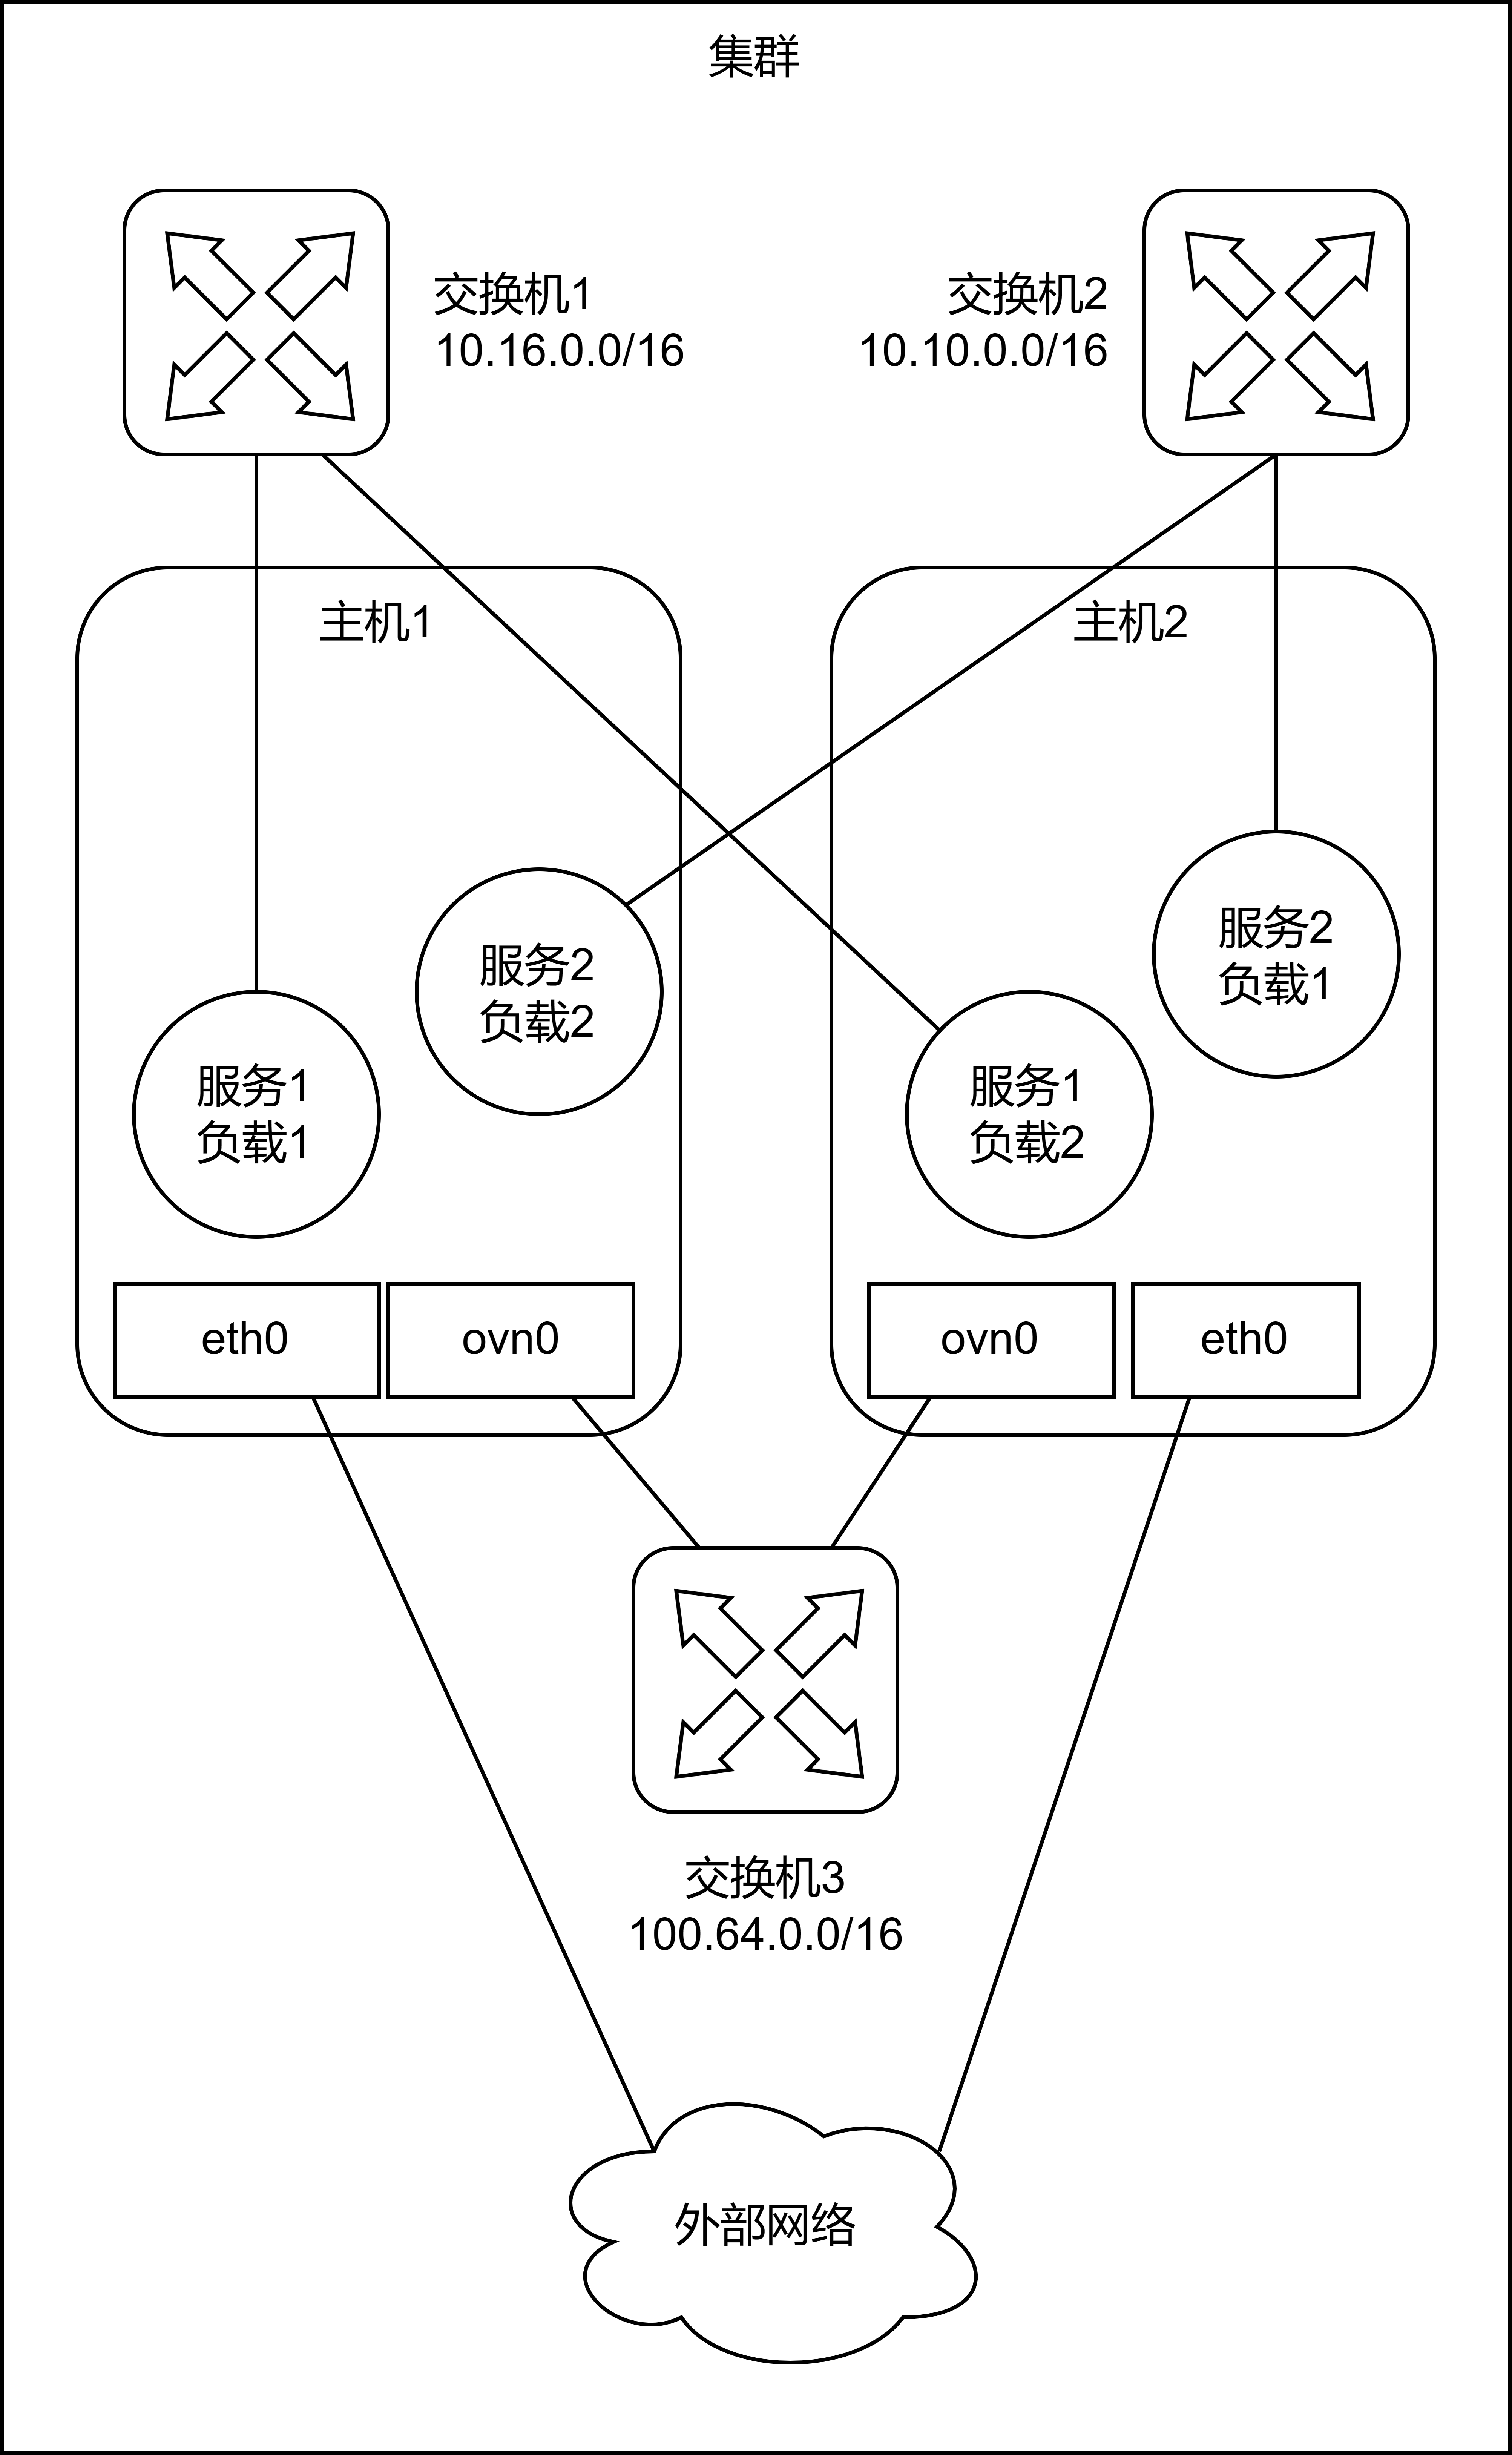
\includegraphics[width=0.50\textwidth]{networking-1}
%     \bicaption{\enspace Kubernetes-dataset 数据集网络拓扑结构}{\enspace Networking Topology of Kubernetes-dataset}
%     \label{fig:networking-1}

% \end{figure}

\begin{table}[t]
    \bicaption{\enspace Kubernetes-dataset 元数据}{\enspace Kubernetes-dataset metadata}
    \label{tab:dataset-metadata}
    \centering
    \footnotesize% fontsize
    \setlength{\tabcolsep}{4pt}% column separation
    \renewcommand{\arraystretch}{1.2}%row space 
    \begin{tabular}{lcccccccc}
        \hline
        流的数量 & 64 599\\
        良性流的数量 & 60 471\\
        ——其中:与攻击场景相关的良性流的数量 & 26 595\\
        恶意流的数量 & 4 128\\
        ——其中:与攻击场景相关的恶意流的数量 & 2 806\\
        ——其中:横向移动流的数量 & 163\\
        流的特征数量 & 79\\
        \hline
    \end{tabular}
\end{table}

}
\chapter{网络流量特征分析和特征重要度评估}{
{
\let\cleardoublepage\relax
}
\label{chap:analyze}

针对基于网络流量的横向移动检测,本文研究和分析了横向移动的原理及其在容器化环境中的行为,以及这些横向移动行为在网络流量特征中的表现。随后,本文对特征进行了最值分析和密度分析,然后进行特征重要度评估。通过这些分析,本文发现对于少量关键的横向移动流量,可进行最值判别;对于大多数横向移动流量,可进行特征筛选,为此,本文进行了特征的重要度评估并进行排序,其评估结果可用于后续模型的训练和测试工作。

\section{横向移动原理分析}
\label{sec:theory}

\subsection{横向移动总体过程}

当攻击者成功进入到目标网络的初始入侵点之后,他往往需要继续访问其初始入侵点以外的其他机器,这是因为他们的主要目标往往不在初始入侵点之上。他们需要继续探索网络以找到他们的目标,然后获得对目标的访问权限。为了达到他们的目标,攻击者可能会安装自己的远程访问工具以控制初始入侵点。

在企业网络中,用户需要使用其凭据才能登录到计算机。然而,攻击者的初始入侵点和主要目标往往不在同一台计算机上,为了达到目标,他们需要切换多个凭据。Hopper \citep{ho2021hopper} 正是利用了这一点,提出了基于凭据切换检验的横向移动检测方法。其他工作 \citep{king2023euler, khoury2023jbeil} 则是基于这些凭据的认证记录,以用户、计算机为节点,凭据认证记录为边,建立动态图模型,以检测横向移动行为。

在移动终端上,攻击者则利用远程服务或串行总线(Universal Serial Bus,USB)来移动到其他设备\citep{mitre2024lm}。例如,攻击者可以使用虚拟专用网(Virtual Private Network,VPN)连接到远程服务,当该服务存在漏洞或后门时,就有可能成功被攻击者利用;攻击者还可以将恶意软件通过 USB 传输并安装到其他计算机上,从而完成一次横向移动操作。

在工业控制系统(Industrial Control Systems,ICS)中,攻击者则可以使用设备中的默认凭据或硬编码凭据、漏洞利用等方式来实施横向移动\citep{mitre2024ics}。

虽然横向移动在不同的环境之下所采用的具体技术不同,但是其共同之处在于攻击者利用这些技术,从当前入侵点访问下一台目标机器。在这些环境中,企业网络环境由于包含了用户的凭据信息,因此为横向移动的检测提供了宝贵的信息,大多数关于横向移动检测的研究工作均在企业网络环境下进行。

\subsection{容器化集群的组件}

在容器化环境中,横向移动的过程包括从对一个容器的给定访问权限获取对集群中各种资源的访问权限,或从容器获取对底层主机的访问权限,或获取对云环境的访问权限。因此,这与容器化集群的组件息息相关。容器化集群的组件如图~\ref{fig:cluster}~所示\citep{k8scomp}。

\begin{figure}[t]
    \centering
    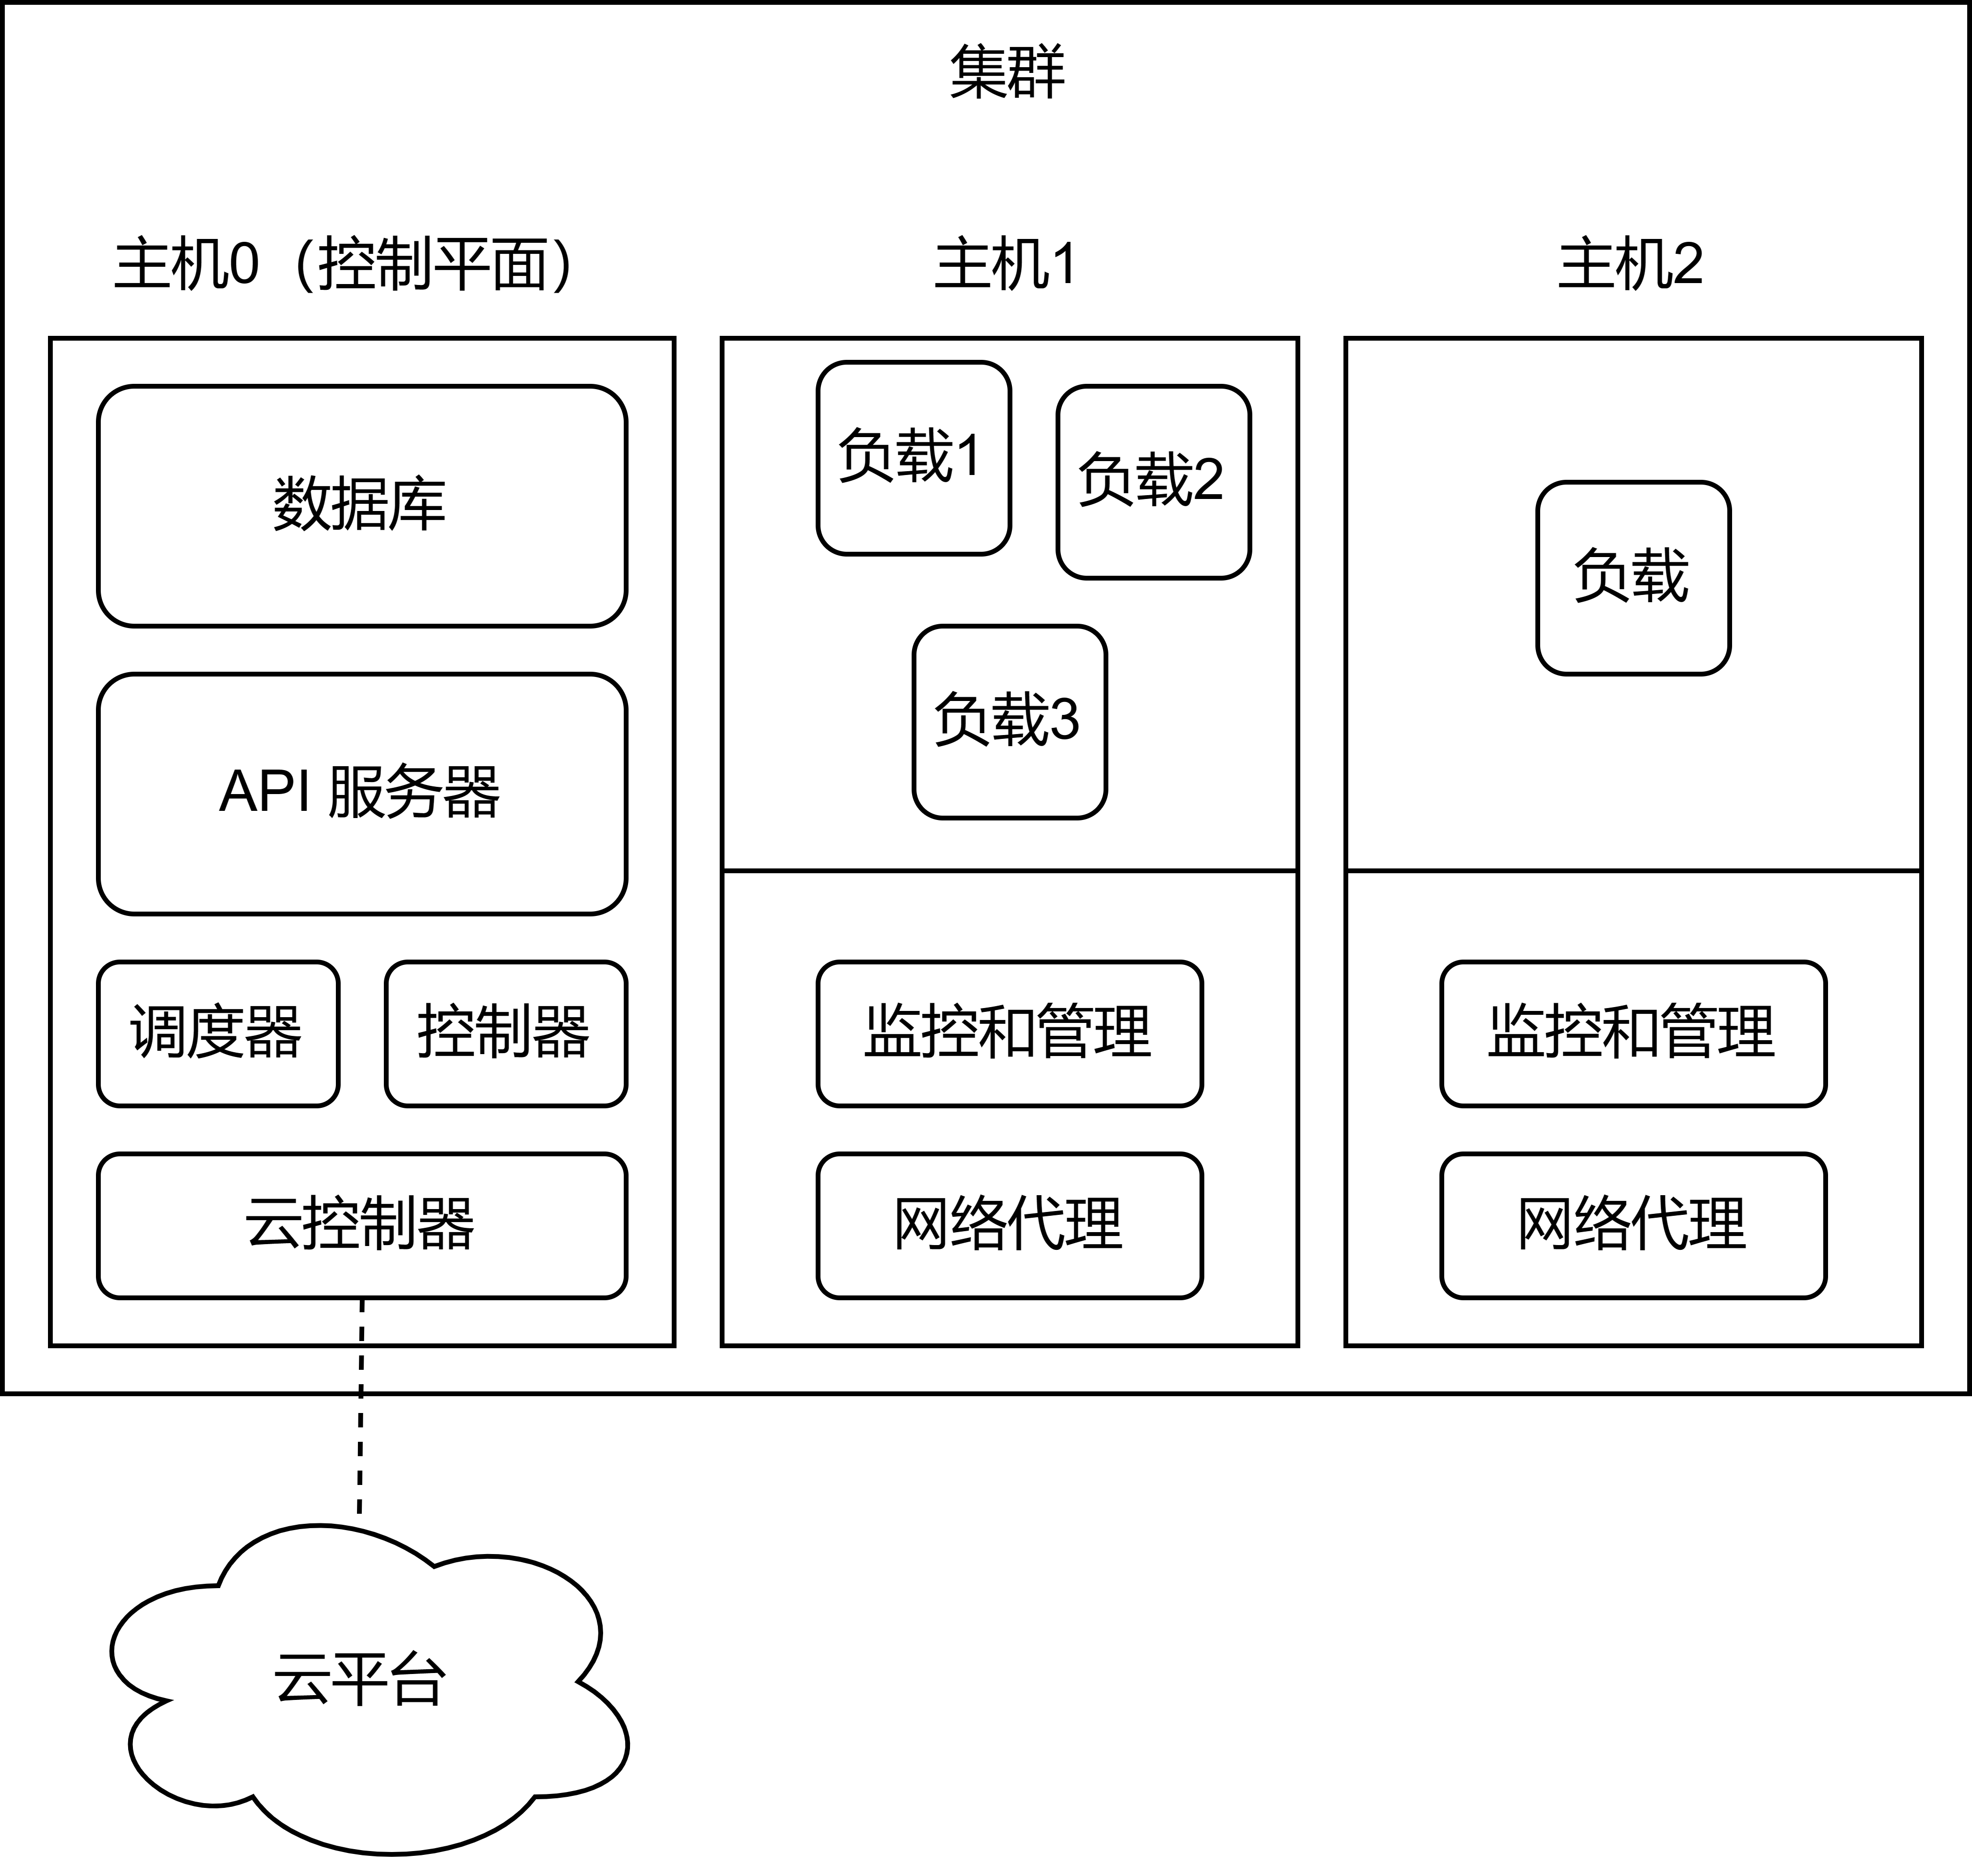
\includegraphics[width=0.7\textwidth]{cluster}
    \bicaption{\enspace 容器化集群组件}{\enspace The components of a containerized cluster}
    \label{fig:cluster}

\end{figure}

容器化集群由若干个主机组成,一般由其中一台主机集中部署控制平面组件,包括 API 服务器、数据库、调度器、控制器、云控制器等;其他主机部署应用程序负载。

在控制平面中,数据库存放集群数据,例如应用程序凭据、云平台的凭据等。API 服务器是控制平面的前端,负责接受请求并处理。调度器负责将应用程序负载调度到集群中的主机上运行。控制器负责处理主机异常时的通知和响应等。云控制器则负责与云平台对接,以便用户通过云平台的仪表板控制容器化集群,并在仪表板上展示容器化集群的状态。

在控制平面以外的主机上运行着多个负载,每个负载包括多个容器。

在容器化集群中,为了实现负载均衡并提高应用程序的可用性,一个应用程序通常对应二个或以上的负载,这些负载共同组成一个对外提供的服务。容器化集群中的服务、负载和主机之间的网络结构如图~\ref{fig:networking}~所示 \citep{k8snet}。

\begin{figure}[t]
    \centering
    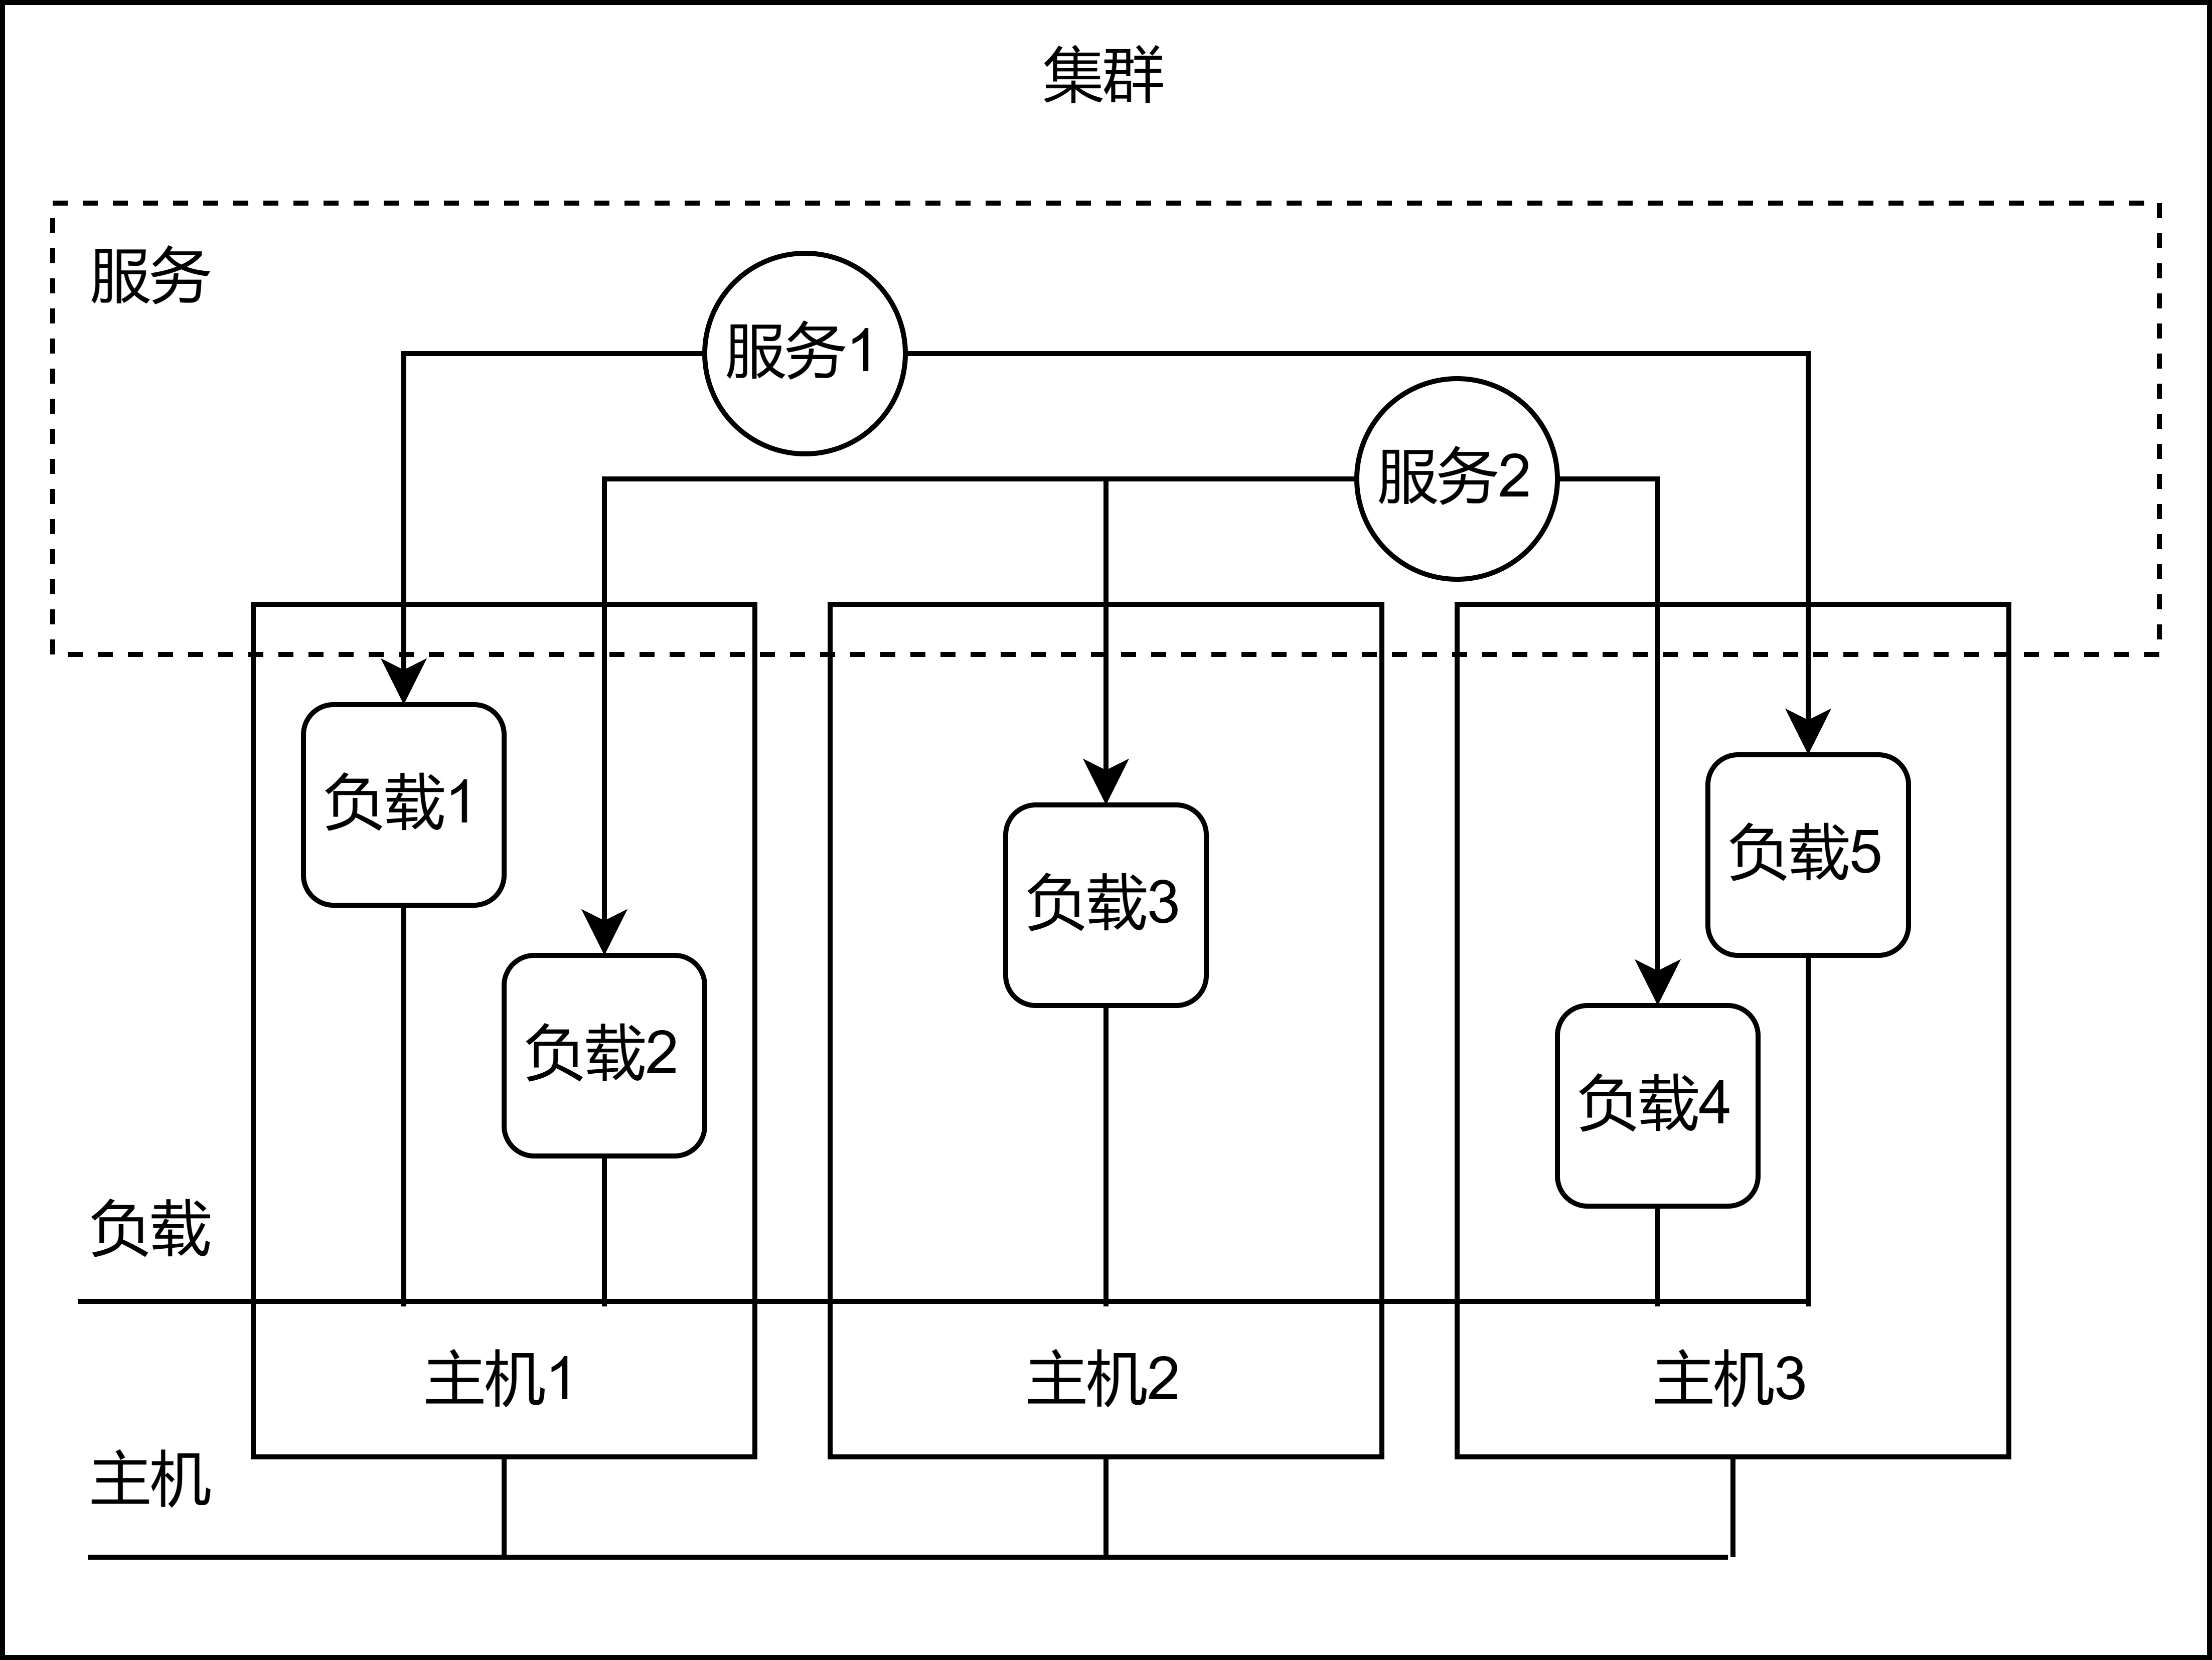
\includegraphics[width=0.80\textwidth]{networking}
    \bicaption{\enspace 容器化集群网络结构}{\enspace The networking architecture of a containerized cluster}
    \label{fig:networking}

\end{figure}

在容器化集群中,API 服务器向集群中的服务分配 IP 地址;不同的负载之间处于同一个网段内,可以直接通过 IP 地址互相访问,由集群的网络插件分配 IP 地址;不同的主机通常配置在同一个网段内,若集群通过云平台部署,则由云控制器分配 IP 地址。

\subsection{容器化集群中的横向移动}

容器化集群的结构为横向移动提供了可能,包括以下行为 \citep{yossi2020threat}:

\begin{itemize}
    \item {从集群移动到云平台:攻击者侵入负载后,利用挂载到负载当中的凭据,非法访问云平台。}
    \item {在负载之间移动:由于容器化集群中的各个负载处于同一个网段内,并在默认情况下允许互相访问,因此攻击者在侵入到其中一个负载之后,可能会非法访问另一个负载。}
    \item {非法请求资源:容器化环境中的负载默认挂载了相应的服务账户凭据。当攻击者侵入负载后,他可以利用该凭据向 API 服务器发起非法请求,以获取集群中的配置文件和其他资源。}
    \item {从负载移动到主机:当上述服务账户具有创建新容器的权限时,攻击者可以创建一个新负载并将主机上的目录挂载到该负载中,从而非法控制主机;也可通过容器逃逸漏洞来控制主机。}
\end{itemize}



% 在容器化集群中,API 服务器作为控制平面的前端,负责处理身份验证和鉴权,工作负载、服务、配置文件等的增、删、改、查操作,既影响集群的行为,也影响集群数据库中存储的敏感信息的机密性、完整性。在上述横向移动行为中,除在负载之间移动以外,其他行为均需和 API 服务器通信;在负载之间的移动虽然不直接与 API 服务器通信,但需要查询集群中的负载情况,此时需要和 API 服务器通信。因此,对 API 服务器相关流量的检测是横向移动检测的重点。

\subsection{横向移动在网络流量中的表现}

在攻击者在容器化环境中执行横向移动时,其网络流量可能发生以下变化:

\begin{itemize}
    \item 负载与外部网络的流量模式发生变化。当攻击者侵入某个负载时,他将在该负载中部署恶意软件或脚本,使该侵入点持久化。这类恶意软件或脚本使该负载处于攻击者的命令与控制(Command and Control,C\&C)服务器的控制之下,从而使该负载的流量模式发生改变。
    \item API 服务器的流量模式发生变化。在容器化集群中,API 服务器作为控制平面的前端,负责处理身份验证和鉴权,工作负载、服务、配置文件等的增、删、改、查操作,既影响集群的行为,也影响集群数据库中存储的敏感信息的机密性、完整性。当攻击者访问非法资源时,API 服务器的网络流量特征发生改变。
    \item 负载之间的流量模式发生变化。当攻击者在不同的负载之间移动时,以往并不互相通信的负载将互相通信;以往互相通信的负载,其网络流量特征发生改变。
    \item 主机的流量模式发生变化。当攻击者从负载移动到主机时,他将在主机上安装恶意软件或脚本。与攻击者侵入负载的情况类似,这也会让主机的流量模式发生改变。
\end{itemize}

\section{网络流量的统计特征}

为了从网络流量中获取统计特征,首先需要将流量聚合为会话。对于 TCP 连接,会话的建立是以一方向另一方发送第一个握手数据包开始,以一方向另一方发送最后一个挥手数据包或重置连接数据包或超时结束。对于 UDP 等无连接协议的数据包,也可以针对具体的应用层协议采用一定的聚合方法,例如对于 DNS 协议而言,可将一次查询请求和其相应的结果返回作为一个会话。会话聚合与单个数据包相比,更能反应网络流量的信息传输情况。

提取统计特征时,可以从基于数据包的特征和基于会话的特征两方面进行提取\citep{WANG2022102542}。基于数据包的特征是在流量数据包级别提取的特征,例如会话中数据包之间的时间差、会话中数据包的大小、会话中的 TCP 标记值统计等。基于会话的功能是在会话级别提取的功能,例如会话持续时间、会话中传输的总字节数、会话中传输的总数据包数等。

若 TCP 流传输了大量数据,需分为多个数据包传输,这些数据包的集合就被称为 bulk。本文参考 CICFlowMeter\citep{engelen2021troubleshooting} 对于 bulk 的聚合方式来选择特征。在进行流的聚合和特征提取时,CICFlowMeter 首先根据流中各数据包的发送时间间隔判断这些数据包能否被聚合为 bulk,然后统计数据包的数量,当数据包达到 4 个时就开始提取 bulk 的特征。因此,与 bulk 相关的特征通常为 $0$,仅在传输数据量较大时大于 $0$,表示此流发生了分包传输。关于分包传输的特征体现了关于大量数据传输的信息。

本文采用的统计特征如表~\ref{tab:dataset-features}~所示。

\begin{table}[t]
    \bicaption{\enspace 网络流量中的统计特征}{\enspace Statistical features of network flows}
    \label{tab:dataset-features}
    \centering
    \footnotesize% fontsize
    \setlength{\tabcolsep}{4pt}% column separation
    \renewcommand{\arraystretch}{1.2}%row space 
    \begin{tabular}{cp{10cm}c}
        \hline
        特征类别 & \centering 特征 & 维度\\
        \hline
        流持续时间 & 流持续毫秒数 & 1\\
        数据包的数量 & 前向数据包数量、后向数据包数量、后向与前向数据包比例、含有至少1字节数据的数据包数量 & 4\\
        数据包的长度 & 前向数据包总长度、后向数据包总长度、前向数据包长度最大值、前向数据包长度最小值、前向数据包长度平均值、前向数据包长度标准差、后向数据包长度最大值、后向数据包长度最小值、后向数据包长度平均值、后向数据包长度标准差、数据包长度最小值、数据包长度最大值、数据包长度平均值、数据包长度标准差 & 14\\
        流速 & 流速(包/秒)、流速(字节/秒)、前向流速(包/秒)、后向流速(包/秒)& 4\\
        数据包的间隔 & 数据包到达时间间隔(Inter-arrival Time,IAT)平均值、IAT标准差、IAT最大值、IAT最小值、前向IAT总和、前向IAT平均值、前向IAT标准差、前向IAT最大值、前向IAT最小值、后向IAT总和、后向IAT平均值、后向IAT标准差、后向IAT最大值、后向IAT最小值 & 14\\
        TCP Flag统计 & 前向PSH、后向PSH、前向URG、后向URG、前向RST、后向RST、FIN、SYN、RST、PSH、ACK、URG、CWR、ECE & 14\\
        数据包首部 & 前向首部长度、后向首部长度 & 2\\
        批量(bulk)传输 & 前向每bulk传输字节数平均值、前向每bulk传输数据包数平均值、前向bulk速率平均值、后向每bulk传输字节数平均值、后向每bulk传输数据包数平均值、后向bulk速率平均值 & 6\\
        TCP窗口 & 前向窗口初始值、后向窗口初始值 & 2\\
        活跃与空闲 & 连续活跃时长平均值、连续活跃时长标准差、连续活跃时长最大值、连续活跃时长最小值、连续空闲时长平均值、连续空闲时长标准差、连续空闲时长最大值、连续空闲时长最小值 & 8\\
        \hline
    \end{tabular}
\end{table}

\section{网络流量特征分析}
\label{sec:analyze}

本节将在 Kubernetes-dataset 数据集的基础上进行网络流量特征分析工作,数据集的详细信息见第~\ref{sec:dataset}~节。

\subsection{最值分析}
\label{sec:extreme}

箱线图能简单反应数据的分布情况,并能够清晰地展示数据的最值。因此,本文为数据集中的各特征绘制箱线图,以进行最值分析。

本文发现,部分特征下,横向移动流量的值域大于良性流量的值域。符合这类分布的特征包括活跃与空闲类特征、批量传输类特征、数据包的长度类特征等。

\begin{itemize}
\item {活跃与空闲类特征

在活跃与空闲类特征中,部分横向移动流量的连续活跃时长最大值、连续活跃时长标准差超过了良性流量在相同特征下的值域。其箱线图如图~\ref{fig:active-max}~所示。

\begin{figure}[t]
    \centering
    \begin{subfigure}[b]{0.48\textwidth}
      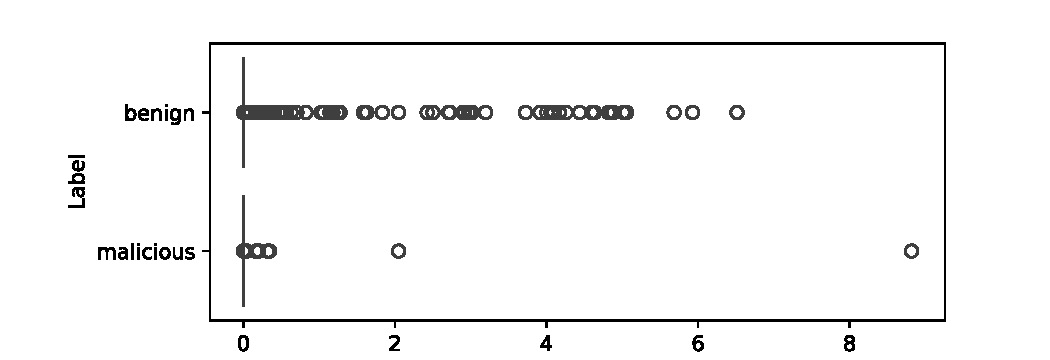
\includegraphics[width=\textwidth]{Active-Max}
      \caption{连续活跃时长最大值}
    \end{subfigure}
    ~
    \begin{subfigure}[b]{0.48\textwidth}
      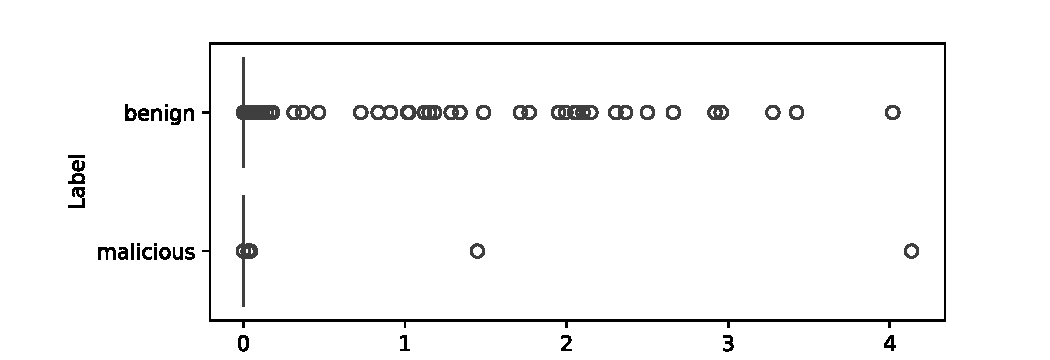
\includegraphics[width=\textwidth]{Active-Std}
      \caption{连续活跃时长标准差}
    \end{subfigure}
    \bicaption{\enspace 连续活跃时长最大值、连续活跃时长标准差箱线图}{\enspace Boxplots of active max and active std}
    \label{fig:active-max}
\end{figure}

从箱线图可以看到,网络流量在该特征下的分布呈现长尾分布,因此箱线图的箱体和线体均集中在图的左侧,几乎不可见;而图的大部分空间均被箱线图的离群点占据。实际上,网络流量在大多数特征下均呈长尾分布。

在这些离群点中,横向移动流量最右侧的离群点比良性流量更靠右,说明其连续活跃时长最大值和标准差更大。说明在集群遭受横向移动攻击后,网络的一些节点之间可能会更频繁地交换数据,这就导致了会话的连续活跃时长最大值更大,同时也带动了其标准差也跟着上升。

}

\item {批量传输类特征

在批量传输类特征中,前向每 bulk 传输字节数平均值、传输数据包数平均值和传输速率呈现出横向移动流量的值域大于良性流量的值域的特点。它们的箱线图如图~\ref{fig:bulk}~所示。

\begin{figure}[t]
    \centering
    \begin{subfigure}[b]{0.48\textwidth}
      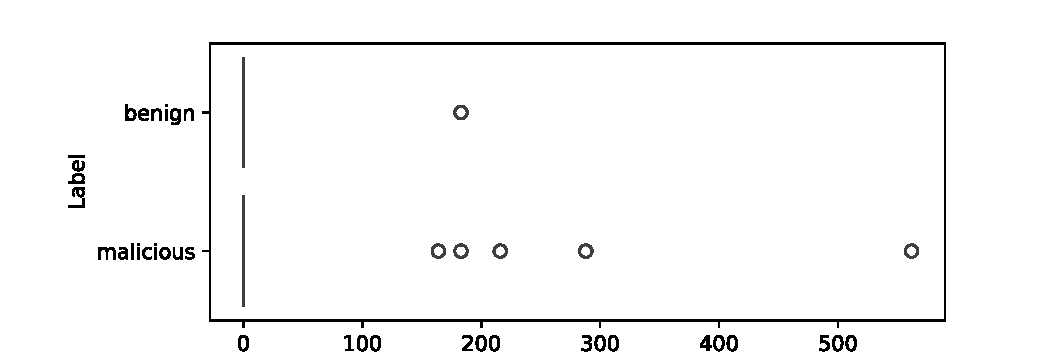
\includegraphics[width=\textwidth]{Fwd-Bytes-Bulk-Avg}
      \caption{前向每 bulk 传输字节数}
    \end{subfigure}
    ~
    \begin{subfigure}[b]{0.48\textwidth}
      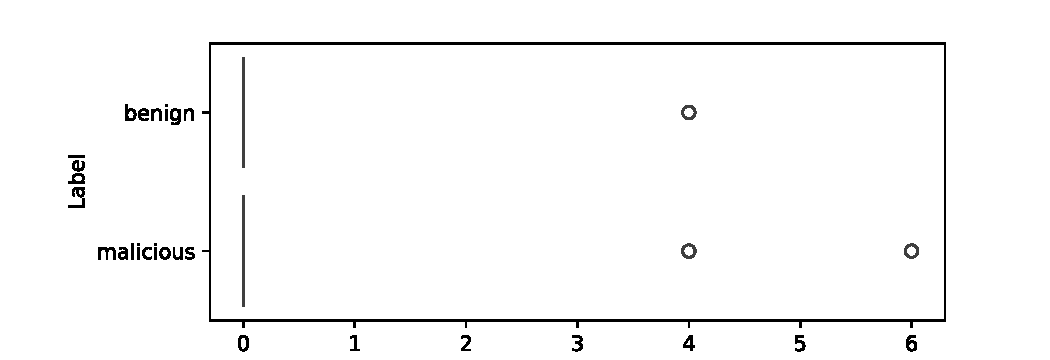
\includegraphics[width=\textwidth]{Fwd-Packet-Bulk-Avg}
      \caption{前向每 bulk 传输数据包数}
    \end{subfigure}
    \\
    \begin{subfigure}[b]{0.48\textwidth}
      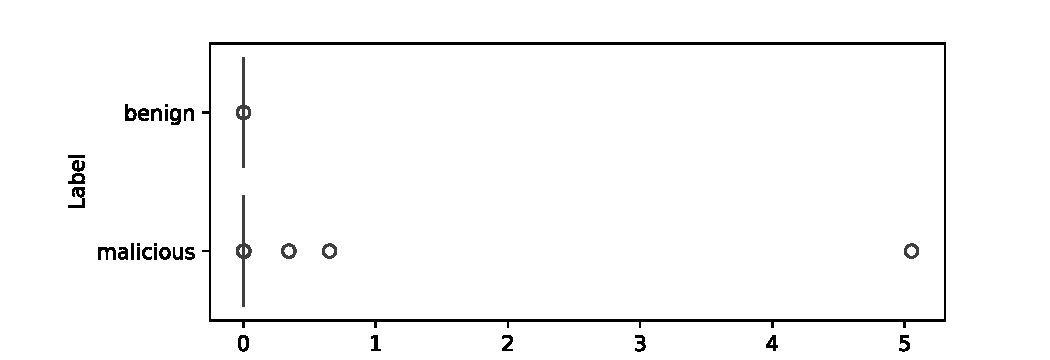
\includegraphics[width=\textwidth]{Fwd-Bulk-Rate-Avg}
      \caption{前向 bulk 传输速率}
    \end{subfigure}
    \bicaption{\enspace 前向批量传输部分特征箱线图}{\enspace Boxplots of some features of bulk data flow}
    \label{fig:bulk}
\end{figure}

结合横向移动攻击的过程,当遭受攻击的负载与攻击者的 C\&C 服务器通信,或从 API 服务器执行资源操作时,可能需要传输大量数据,以便安装恶意软件或控制集群,这会使得相应的特征的值上升。
}

\item {数据包的长度类特征

在数据包的长度类特征中,前向数据包长度最大值也可呈现出类似特点。它的箱线图如图~\ref{fig:fwd-packets-length-max}~所示。

\begin{figure}[t]
    \centering
    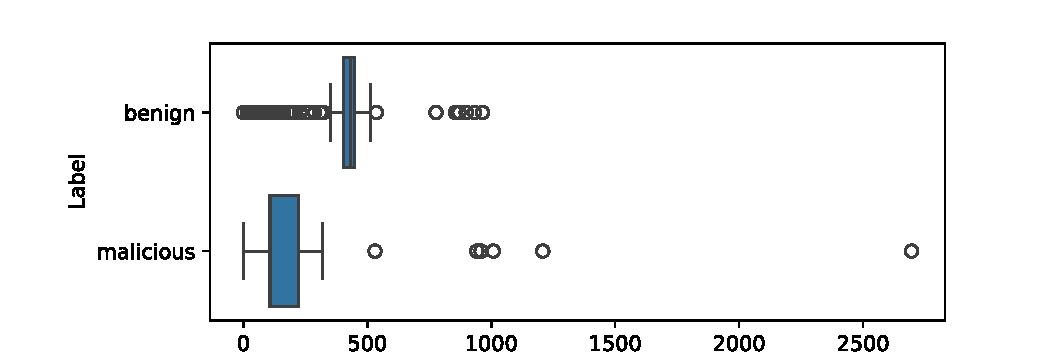
\includegraphics[width=0.48\textwidth]{Fwd-Packet-Length-Max}
    \bicaption{\enspace 前向数据包长度最大值箱线图}{\enspace Boxplot of fwd packets length max}
    \label{fig:fwd-packets-length-max}
\end{figure}
}

与上一类特征类似,结合横向移动攻击的过程,可以推断,当负载遭受攻击之后,将与攻击者的 C\&C 服务器之间传输大量数据,或向 API 服务器请求大量数据,使数据包长度的最大值上升。不过,该特征同时受到网络中最大传输单元(Maximum Transmission Unit,MTU)的影响,因此其适合与批量传输类特征一同使用,呈互补关系。

\end{itemize}

大多数特征下,横向移动流量的值域与良性流量的值域大致相同,或横向移动流量的值域小于良性流量的值域。以 IAT 平均值和前向每秒传输数据包数为例,其箱线图如图~\ref{fig:flow-iat-mean}~所示。

\begin{figure}[t]
    \centering
    \begin{subfigure}[b]{0.48\textwidth}
      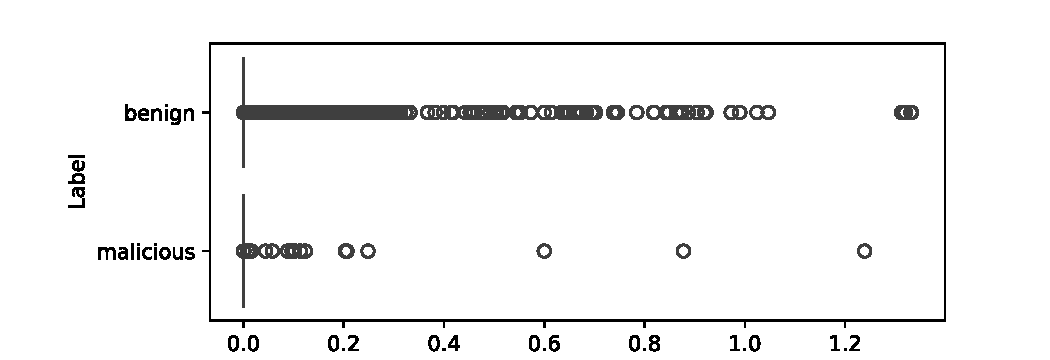
\includegraphics[width=\textwidth]{Flow-IAT-Mean}
      \caption{IAT 平均值}
    \end{subfigure}
    ~
    \begin{subfigure}[b]{0.48\textwidth}
      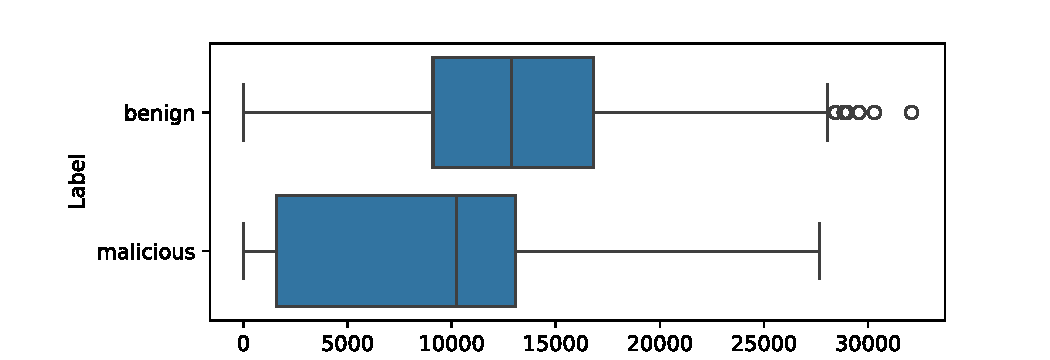
\includegraphics[width=\textwidth]{Fwd-Packets-s}
      \caption{前向每秒传输数据包数}
    \end{subfigure}
    \bicaption{\enspace IAT 平均值、前向每秒传输数据包数箱线图}{\enspace Boxplots of IAT mean and fwd packets/s}
    \label{fig:flow-iat-mean}
\end{figure}

此类特征难以区分横向移动流和良性流,因此不能直接被用来识别横向移动,需要采取机器学习等更高级的方式。

通过上述最值分析,本文发现,少量横向移动流量可以用最值法检出,这些横向移动流量代表了负载受遭受攻击之后,其与 API 服务器、与外部网络通信的流量模式发生了改变。然而,大多数横向移动流量仍不能检测出来,因此本文将进行密度分析,观察大多数流量的分布情况。

\subsection{密度分析}
\label{sec:distplots}

与箱线图相比,而直方图和密度图可以提供更全面的信息,因此,本小节将使用直方图和密度图(下文统称为分布图)进行密度分析。

虽然大多数特征呈现长尾分布,但也有少量特征不遵循长尾分布,可以不去除离群点而直接观察其分布图。这包括流速类特征、数据包的长度类特征等。

\begin{itemize}
\item {流速类特征

流速(包/秒)、前向流速(包/秒)、后向流速(包/秒)的分布图如图~\ref{fig:flow-rate}~所示。

\begin{figure}[t]
    \centering
    \begin{subfigure}[b]{0.48\textwidth}
      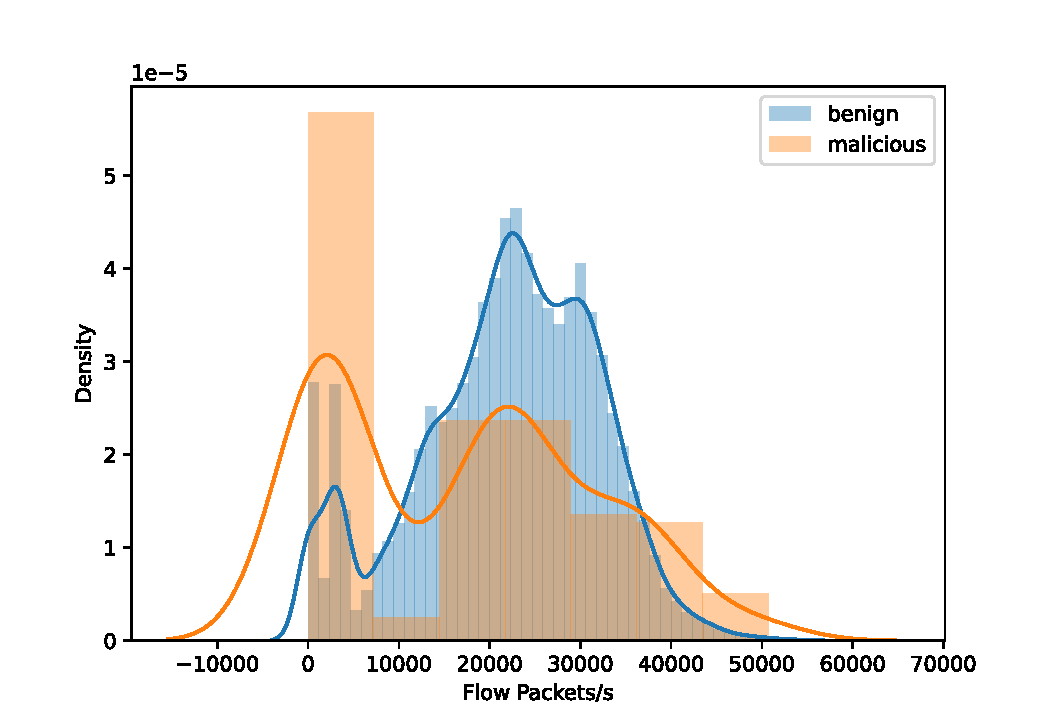
\includegraphics[width=\textwidth]{Flow-Packets-s}
      \caption{流速(包/秒)}
    \end{subfigure}
    ~
    \begin{subfigure}[b]{0.48\textwidth}
      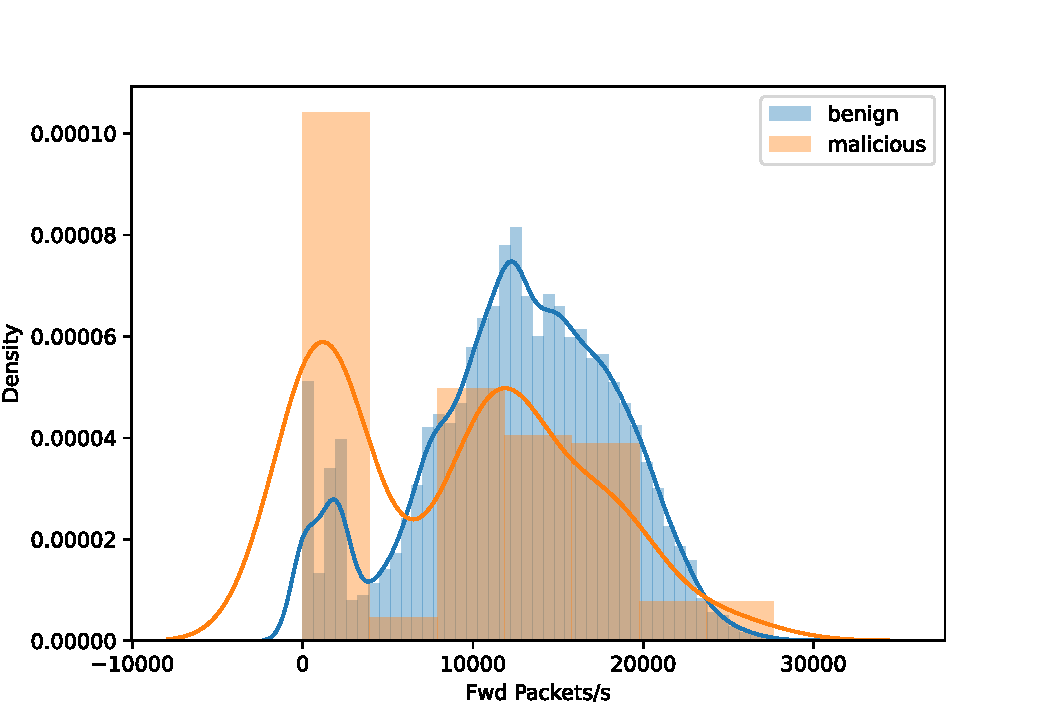
\includegraphics[width=\textwidth]{Fwd-Packets-s-1}
      \caption{前向流速(包/秒)}
    \end{subfigure}
    \\
    \begin{subfigure}[b]{0.48\textwidth}
      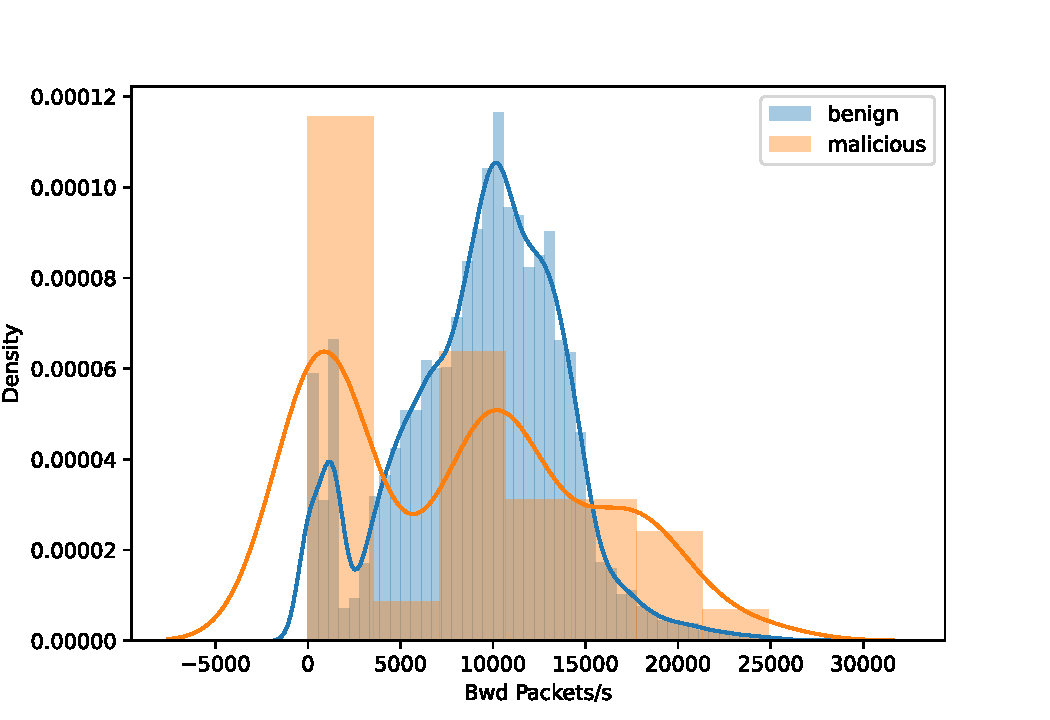
\includegraphics[width=\textwidth]{Bwd-Packets-s}
      \caption{后向流速(包/秒)}
    \end{subfigure}
    \bicaption{\enspace 流速部分特征分布图}{\enspace Distribution plots of some features of flow rate}
    \label{fig:flow-rate}
\end{figure}

横向移动流量和良性流量的流速(包/秒)、前向流速(包/秒)、后向流速(包/秒)特征均呈双峰分布,其中一峰集中于 0 附近,说明传流速慢的会话占一部分比例,这些会话可能是长连接会话;另一峰则在 10 000 至 40 000 包/秒之间,这些会话则是以数据传输为主的会话。两者的密度分布差异说明,与良性流量相比,横向移动流量的数据传输需求较低。
}

\item {数据包的长度类特征

前向数据包长度最大值、平均值、标准差的分布图如图~\ref{fig:fwd-packet-length}~所示。

\begin{figure}[t]
    \centering
    \begin{subfigure}[b]{0.48\textwidth}
      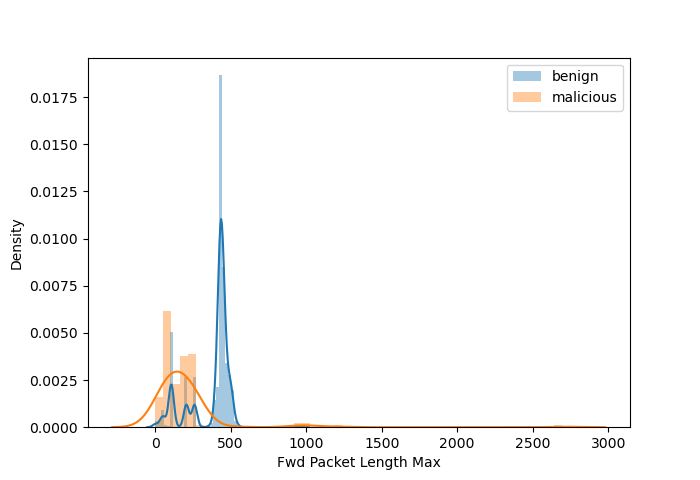
\includegraphics[width=\textwidth]{Fwd-Packet-Length-Max-1}
      \caption{前向数据包长度最大值}
    \end{subfigure}
    ~
    \begin{subfigure}[b]{0.48\textwidth}
      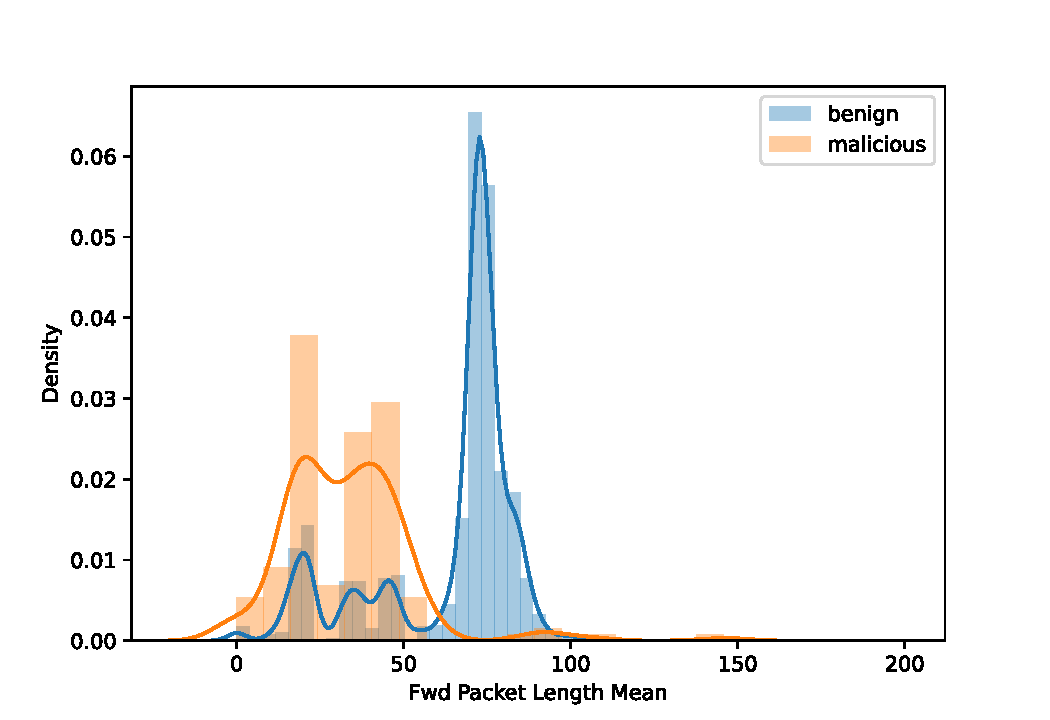
\includegraphics[width=\textwidth]{Fwd-Packet-Length-Mean}
      \caption{前向数据包长度平均值}
    \end{subfigure}
    \\
    \begin{subfigure}[b]{0.48\textwidth}
      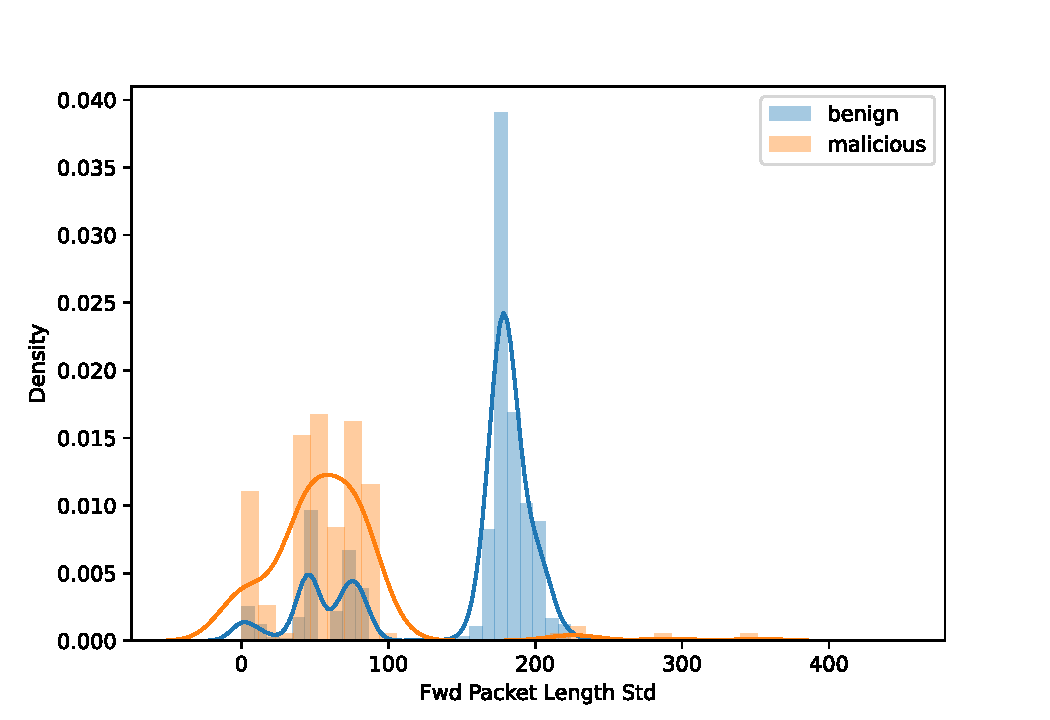
\includegraphics[width=\textwidth]{Fwd-Packet-Length-Std}
      \caption{前向数据包长度标准差}
    \end{subfigure}
    \bicaption{\enspace 前向数据包长度最大值、平均值和标准差分布图}{\enspace Distribution plots of fwd packet length max, mean and std}
    \label{fig:fwd-packet-length}
\end{figure}

横向移动流量的分布呈单峰分布,集中在 0 附近;良性流量的分布则呈双峰分布,其中一峰集中于 0 附近,另一峰则在中部。当传输大量数据时,数据包的长度较长,因此数据包长度较短时,说明此时执行的可能是简单查询操作或发起简单指令。这与 API 服务器的资源操作是匹配的。大部分横向移动流量对大量数据传输没有需求;但是,这并不排除个别横向移动流量传输大量数据的情况(见第~\ref{sec:extreme}~节)。

\item {数据包的数量类特征

在数据包的数量类特征中,后向与前向数据包比例呈现三峰分布,其分布图如图~\ref{fig:down-up-ratio}~所示。

\begin{figure}[t]
    \centering
    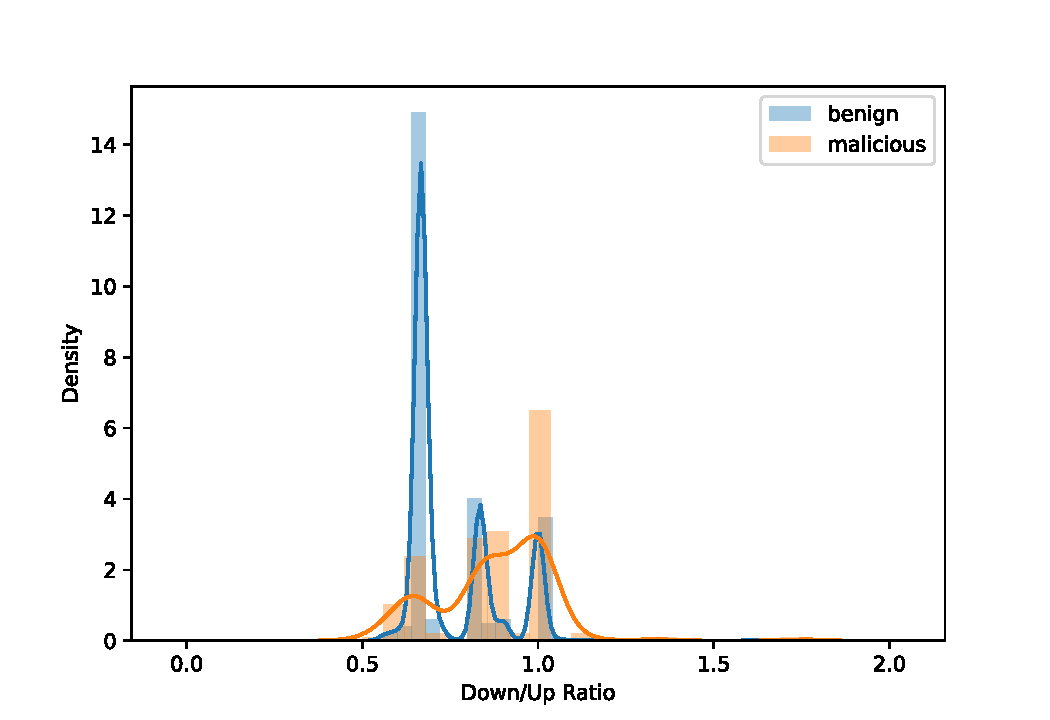
\includegraphics[width=0.48\textwidth]{Down-Up-Ratio}
    \bicaption{\enspace 后向与前向数据包比例分布图}{\enspace Distribution plot of down/up ratio}
    \label{fig:down-up-ratio}
\end{figure}

在良性流量中,大部分会话的后向数据包数量小于前向数据包,此时会话以上传为主。在 TCP 会话中,有相当一部分数据包用于维护连接,后向数据包和前向数据包数量相近,因此该比例越接近 1 时,数据包数量往往越小,说明会话中用于维护连接的数据包所占比例越大。因此,横向移动流量与良性流量的不同之处在于,横向移动流量有效传输的数据不多,它对容器化集群所提供的服务没有兴趣。
}
}
\end{itemize}

其余的大部分特征符合长尾分布,或其分布范围较窄,从分布图中难以获取有效信息。以 TCP SYN 统计和流速(字节/秒)为例,它们的分布图如图~\ref{fig:syn-flag-count}~所示。

\begin{figure}[t]
    \centering
    \begin{subfigure}[b]{0.48\textwidth}
      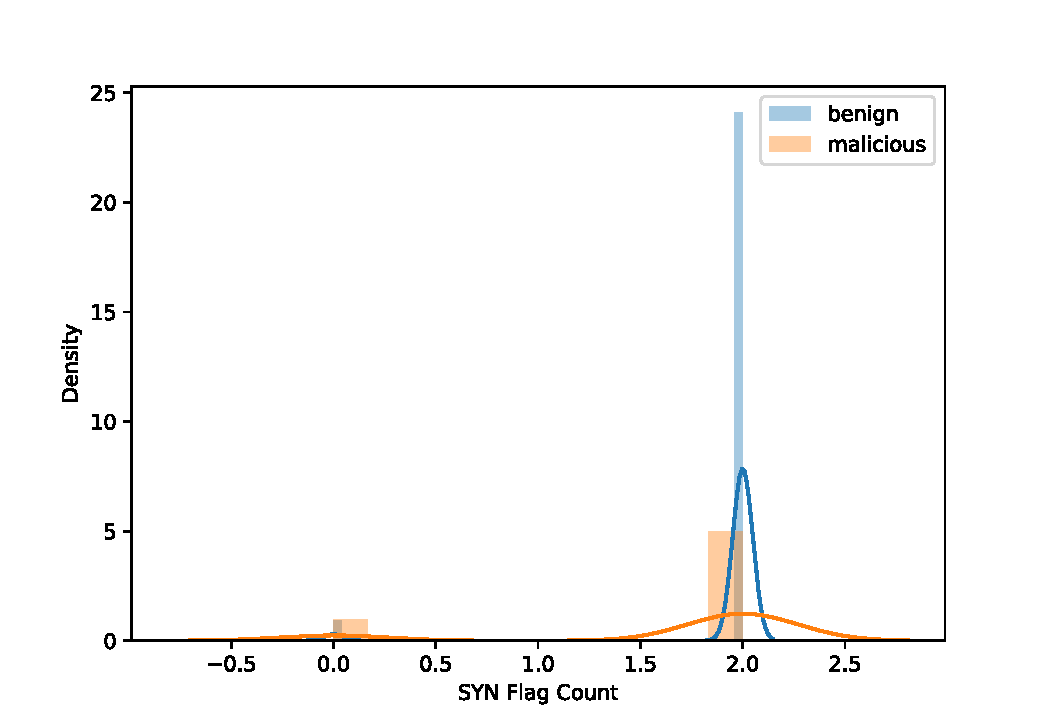
\includegraphics[width=\textwidth]{SYN-Flag-Count}
      \caption{TCP SYN 统计}
    \end{subfigure}
    ~
    \begin{subfigure}[b]{0.48\textwidth}
      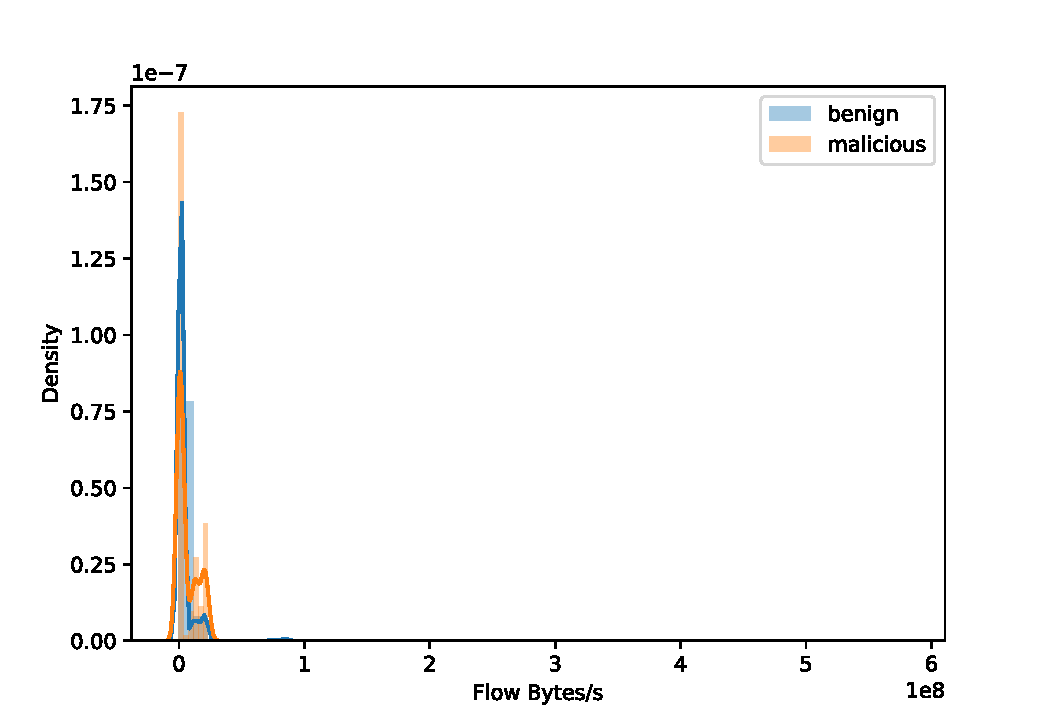
\includegraphics[width=\textwidth]{Flow-Bytes-s}
      \caption{流速(字节/秒)}
    \end{subfigure}
    \bicaption{\enspace TCP SYN 统计、流速(字节/秒)分布图}{\enspace Distribution plots of SYN flag count and flow bytes/s}
    \label{fig:syn-flag-count}
\end{figure}

\subsection{小结}

本节通过最值分析和密度分析,对横向移动流量与良性流量的差异进行了评估。通过最值分析,发现少数横向移动流量的分布超出了良性流量的范围,并且它们反映了负载遭受攻击后与 API 服务器及外部网络的访问模式发生了变化。通过密度分析,发现横向移动行为与良性流量相比,通常不需要很高的数据传输量,这使得大部分横向移动流量隐蔽在良性流量之间。此外,大部分网络流量特征呈长尾分布。因此,需要采用机器学习的方式进行特征重要度评估,进一步挖掘其中的信息。

\section{基于机器学习的网络流量特征重要度评估}
\label{sec:filter}

使用机器学习进行数值连续型特征的筛选,通常可以采用决策树方法,也可以挖掘特征与目标变量之间的关联性。

决策树由根节点、内部节点和叶子节点组成。根节点代表整个数据集,每个内部节点代表对一个特征的判断。用于分类模型时,每个叶子节点代表一个决策分数。然而,单棵决策树通常容易过拟合、准确性较低,因此通常使用多棵决策树集成学习的方法。

多棵决策树的集成学习有两种方式:

\begin{itemize}
    \item 随机森林基于装袋(bagging)方法,从训练数据中随机抽取多个子集,对每个子集训练一棵决策树,然后将其组合得到最终的预测结果。
    \item 梯度提升决策树基于提升(boosting)方法,训练多棵决策树,其中每一棵决策树训练完成后,对该树错误分类的样本给予更高的权重,以训练下一棵决策树。
\end{itemize}

为了计算特征重要度,通常采用基尼系数。它计算的是数据集中的样本属于不同类别的概率,基尼系数越大,说明数据集越不纯,即样本属于不同类别的概率越高。对集成学习中每棵决策树的相应特征的节点计算基尼系数的降低值,然后作平均,可以得出各个特征的重要度指标。

挖掘特征与目标变量之间的关联性时,对于分类问题,一般可使用卡方检验、F检验或互信息量检验。然而,卡方检验只适用于离散型特征,而网络流量的特征主要包含连续型变量,因此不适用卡方检验。F检验要求特征服从正态分布,根据第~\ref{sec:distplots}~节中的分布图,这些特征与正态分布差异较大,因此不适用F检验。互信息量检验可用于连续型特征,对特征分布没有要求,因此可以采用互信息量检验的方法。

互信息量用于评价两个随机变量之间的依赖程度,若一个随机变量已知时,另一个变量的不确定性(熵)减少,则这两个随机变量的互信息量较高。互信息的计算公式\eqref{eq:multi-info}如下:

\begin{figure}[t]
    \centering
    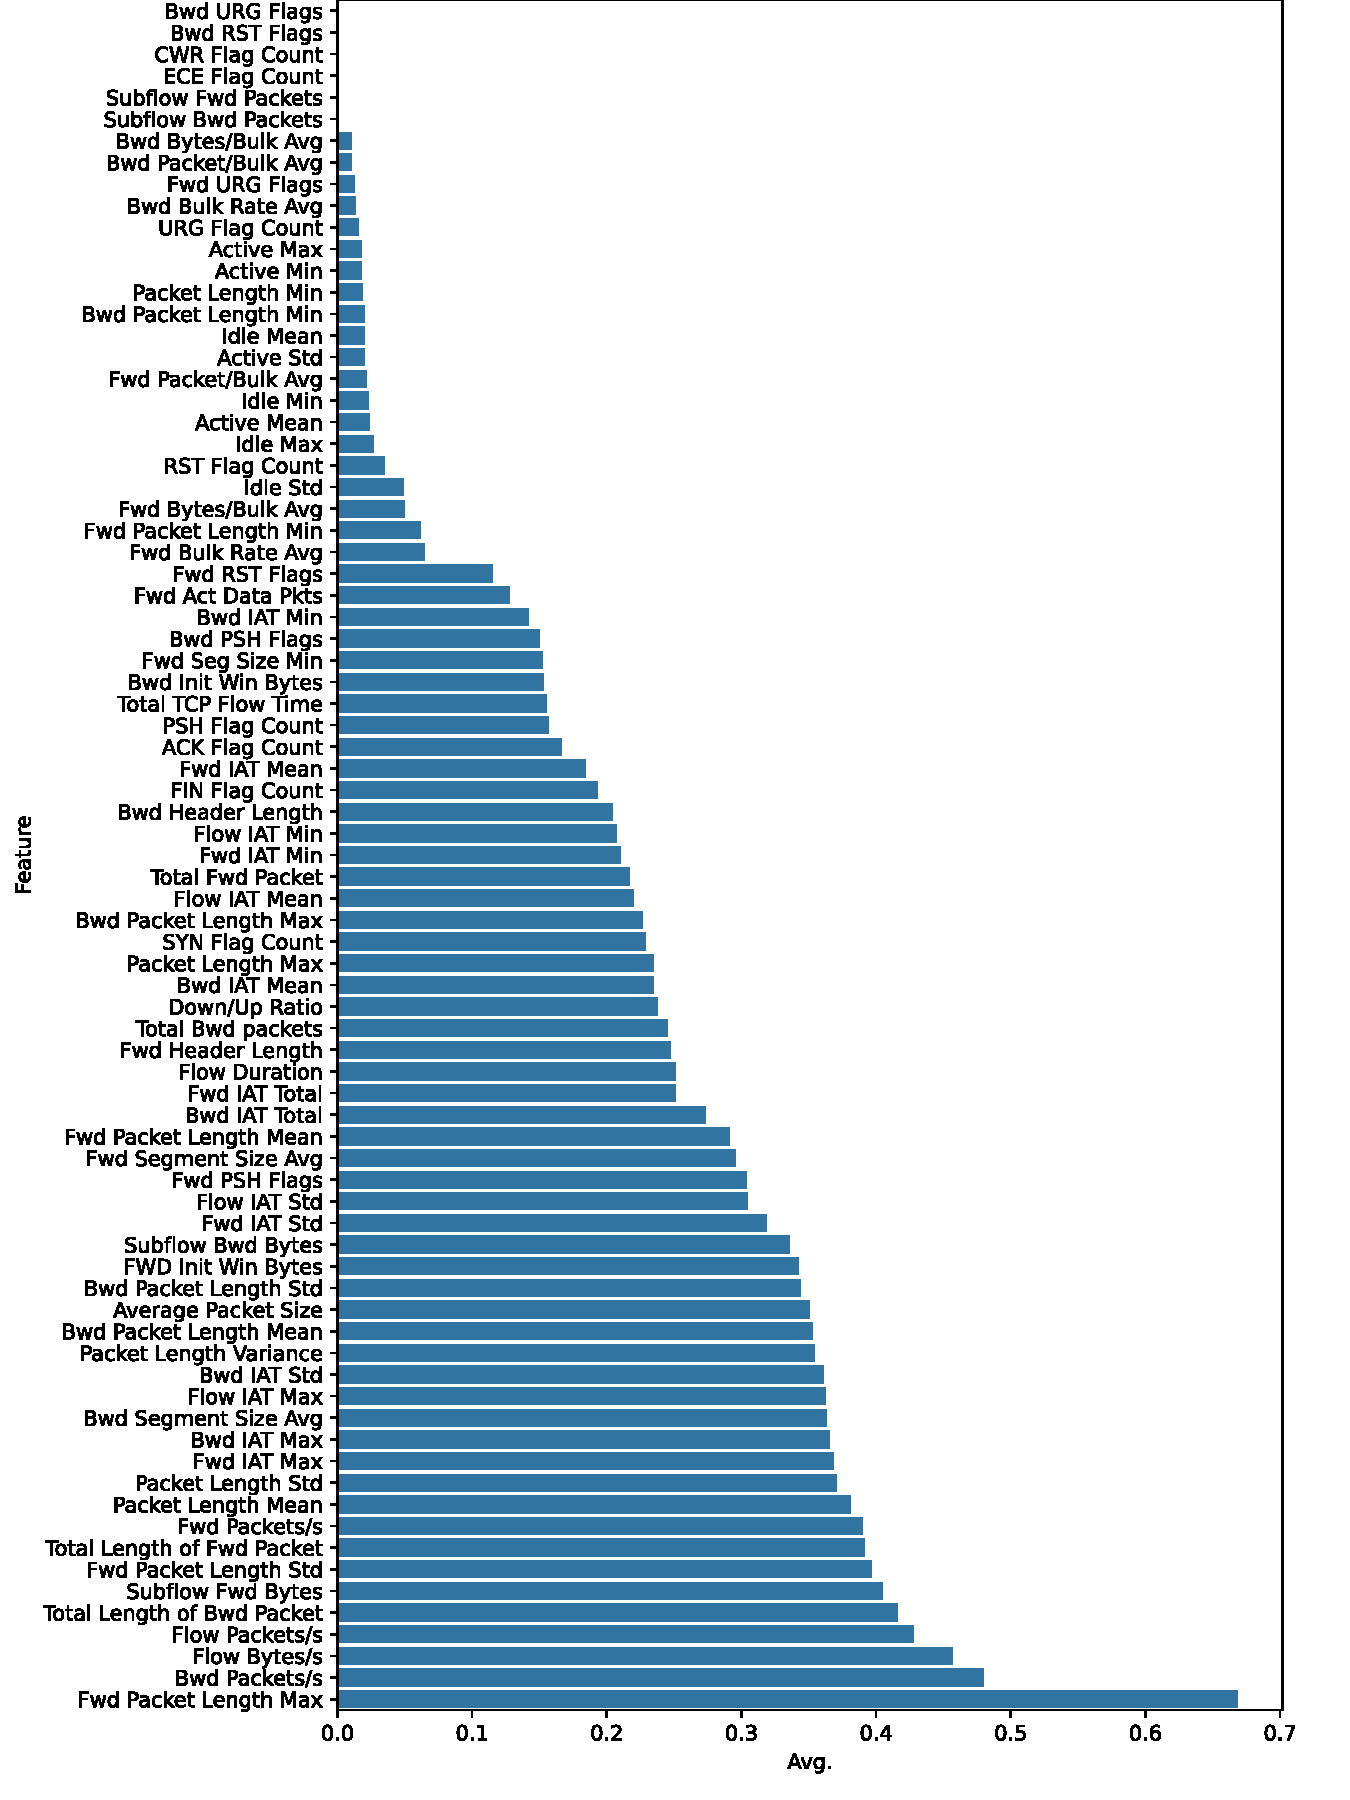
\includegraphics[width=1.0\textwidth]{unimportance}
    \bicaption{\enspace 网络流量中各特征的重要度}{\enspace The importance of features of flows}
    \label{fig:unimportance}

\end{figure}

\begin{equation}
    \label{eq:multi-info}
    \begin{split}
        I(X;Y) &= \sum_{x \in X} \sum_{y \in Y} p(x,y) \log \frac{p(x,y)}{p(x)p(y)}.
    \end{split}
\end{equation}

在公式\eqref{eq:multi-info}中,$X$ 和 $Y$ 表示两个变量,$p(x,y)$ 表示这两个变量的联合概率分布,$p(x)$、$p(y)$ 表示边缘概率分布。该公式用于计算 $X$ 和 $Y$ 的依赖程度。通过评价网络流量各特征与其标签的依赖程度,即可得到特征的重要度。

本文通过使用梯度提升决策树、随机森林、互信息量分别得到各特征的重要度,并缩放至$\left[0,1\right]$区间后,按其平均值从低到高排列,如图~\ref{fig:unimportance}~所示。

三个模型一致认为后向 URG、后向 RST、CWR、ECE、前向子流数据包数、后向子流数据包数等六个特征的重要度为零,因此可以从数据集中删除。前向数据包长度最大值的重要度最大,这也验证了第~\ref{sec:analyze}~节中的讨论。其他特征的重要度则呈梯级分布。这些特征的重要度将在后续的模型设计中得到应用。

\section{实验评估}

由于后续章节将使用基于流量预测的方法进行横向移动检测,本节将使用 GRU 模型来验证特征重要度评估方法,将最不重要的若干个特征删除,并与另一种常见的特征降维方法,主成分分析(Principal Component Analysis,PCA),进行对比。数据集和评估指标分别如第~\ref{sec:experiment-dataset}~节和第~\ref{sec:kpi}~节所述。实验对比了全量特征(79维)、筛除一部分特征(剩余57维)和使用 PCA 压缩到57维的结果,如表~\ref{tab:analyze-expreiment-result}~所示。

\begin{table}[!htbp]
    \bicaption{\enspace 特征降维方法对比实验结果}{\enspace Comparison results of feature dimensionality reduction}
    \label{tab:analyze-expreiment-result}
    \centering
    \footnotesize% fontsize
    \setlength{\tabcolsep}{4pt}% column separation
    \renewcommand{\arraystretch}{1.2}%row space 
    \begin{tabular}{ccccccccc}
        \hline
        实验项目 & 特征维度 & TPR & FPR & F1 & AUC\\
        \hline
        全量特征 & 79 & 0.7239 & 0.2814 & 0.0934 & 0.8080\\
        筛除一部分特征 & 57 & 0.7423 & 0.2543 & 0.1046 & 0.8113\\
        PCA & 57 & 0.7178 & 0.2795 & 0.0932 & 0.8038\\
        \hline
    \end{tabular}
\end{table}

结果表明,使用本文提出的方法进行降维,去除无关特征后,模型的性能有所提高,AUC 达到 0.8113,四个指标均为最优;若使用 PCA 进行降维,模型性能反而下降,并且 PCA 丢失了降维方法的可解释性。因此,本文提出的特征重要度评估方法是有效的,并且比 PCA 方法更优,后续在第~\ref{sec:feature-filter}~节还将进行进一步验证。

\section{本章小结}

本章首先对横向移动原理进行分析,指出了横向移动将导致容器化集群中的负载、主机和 API 服务器的流量模式发生改变。接着,本文通过特征分析,指出了这种改变主要存在于两个方面:对于少量但是关键的横向移动流量而言,它会传输大量数据,导致部分批量传输特征、数据包长度特征的值超出了良性流量的值域,这是因为负载处在攻击者的 C\&C 服务器的控制之下,攻击者在负载上安装恶意软件或脚本,并从 API 服务器窃取关键信息;对于大部分横向移动流量而言,它们的特征分布与良性流量也有所差异,横向移动往往具有更低的数据传输需求。最后,本文通过基于决策树和互信息量检验的特征重要度评估,验证了特征分析的结论,并得到了各特征的评估分数,这将在后续的模型设计中得到应用。
}
\chapter{容器化环境中的横向移动时空特性分析}{
{
\let\cleardoublepage\relax
}
\label{chap:embedding}

% 为了通过网络流量来检测容器化环境中的横向移动,我们需要了解横向移动的原理,以及横向移动在网络流量特征中的表现。本章将首先介绍横向移动的原理,讨论容器化环境中横向移动的特点,分析横向移动流量与良性流量的特征差异,然后在数据集上进行特征分析,最后使用决策树和互信息量检验,进行特征重要度评估。

横向移动除了导致流量的特征与良性流量相比有所不同以外,还会对网络的拓扑结构产生影响;此外,也会对网络流量随时间的变化产生影响。

本文研究和分析了容器化环境中的网络流量拓扑结构,发现横向移动行为会导致网络流量拓扑结构发生改变。例如,攻击者发起横向移动攻击后,从未与 API 服务器通信的负载开始与 API 服务器通信。因此,通过检测拓扑结构的变化可以检测出关键的横向移动流量。

对于大多数横向移动流量,本文进行了空间特征嵌入方法和时间特征嵌入方法研究,进一步挖掘网络流量中包含的信息,得到空间和时间特征嵌入向量,用于后续模型的输入。

\section{横向移动对网络流量拓扑结构的影响}
\label{sec:topology}

容器化环境中的网络流量服从一定的规律,可以从中挖掘一定的空间特征。如果将流量建模为图,图上的节点代表 IP 地址和端口的组合\footnote{IP 地址相同、端口号大于 32768 的,聚合为同一个节点。},边代表节点之间产生的流量,便可以利用图机器学习的方式挖掘这些空间特征,并通过节点的嵌入向量表现出来。

从第~\ref{sec:theory}~节的分析,可以看到,当攻击者侵入容器化集群中的负载之后,他可能移动到其他负载、主机等地方,并且将该负载与攻击者的 C\&C 服务器建立连接,以便部署恶意软件并进行控制。因此,横向移动会导致网络流量拓扑结构发生如下改变:

\begin{itemize}
    \item 负载与 API 服务器之间的连接关系发生变化。正常情况下不需要与 API 服务器通信的负载在遭受攻击后开始与 API 服务器通信,以便获取集群的配置文件并执行资源操作。
    \item 负载之间的连接关系发生变化。正常情况下不需要通信的负载之间发生通信,这表明攻击者在负载之间进行了横向移动。
    \item 容器化集群中出现了新的负载,且该负载与集群配置的扩容策略等无关。这种情况说明,攻击者通过 API 服务器非法创建了一个新的负载,该负载可能带有特殊权限,以便攻击者从负载移动到主机上。
    \item 负载与外部网络之间的连接关系发生变化。当正常情况下不需要与外部网络通信的负载开始与外部网络通信时,或者负载开始访问其以前从未访问过的网段时,说明该负载被攻击者控制,并与攻击者的 C\&C 服务器通信。
    \item 主机与外部网络之间的连接关系发生变化。和上述情况类似,当攻击者从负载移动到主机上时,主机将开始处于攻击者的 C\&C 服务器之下。
\end{itemize}

\section{网络流量的拓扑结构分析}
\label{sec:topology}

为了更加具体地研究横向移动对网络流量拓扑结构的影响,本文继续在 Kubernetes-dataset 数据集上进行分析,数据集的详细介绍见第~\ref{sec:dataset}~节。

首先,将数据集中的良性流建模为图,然后通过 NetworkX\citep{networkx} 可视化,如图~\ref{fig:benign-structure}~所示。

\begin{figure}[t]
    \centering
    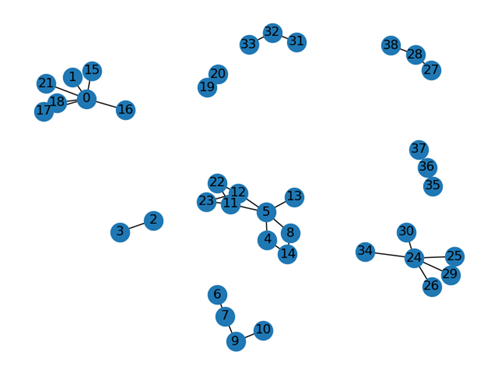
\includegraphics[width=0.75\textwidth]{benign-structure}
    \bicaption{\enspace 良性流的网络拓扑结构}{\enspace Topological diagram of benign flows}
    \label{fig:benign-structure}

\end{figure}

可以看到,在容器化集群中,各节点分为 9 个组,并在组内进行通信,这些通信表现出了不同的通信模式。接下来对不同的通信模式进行分析。

(一)主机与负载之间的通信。节点 0、1、15、16、17、18、21 之间的通信属于此类。这些节点的 IP 地址和端口如表~\ref{tab:benign-structure-1}~所示。

\begin{table}[!htbp]
    \bicaption{\enspace 良性流中主机与负载之间通信的相关节点}{\enspace Nodes related to communications between hosts and pods}
    \label{tab:benign-structure-1}
    \centering
    \footnotesize% fontsize
    \setlength{\tabcolsep}{4pt}% column separation
    \renewcommand{\arraystretch}{1.2}%row space 
    \begin{tabular}{cccccc}
        \hline
        编号 & IP 地址 & 端口\\
        \hline
        0 & 100.64.0.2 & \geq 32768\\
        1 & 10.16.0.45 & 1880\\
        15 & 10.16.0.5 & 8080\\
        16 & 10.16.0.4 & 8181\\
        17 & 10.16.0.4 & 8080\\
        18 & 10.16.0.7 & 7472\\
        21 & 10.16.0.5 & 8181\\
        \hline
    \end{tabular}
\end{table}

在这些节点中,节点 0 为主机节点,其余节点为负载节点。其中,节点 16、17 和 15、18 分别部署了 HTTP 服务,节点 1 部署了 Node-RED 服务,节点 18 部署了其他服务。主机是以客户端的身份向这些负载通信的,也就是说这些流量代表了对负载中部署的应用程序的访问。

(二)API 服务器与负载之间的通信。节点 4、5、8、11、12、13 之间的通信属于此类。这些节点的 IP 地址和端口如表~\ref{tab:benign-structure-2}~所示。

\begin{table}[!htbp]
    \bicaption{\enspace 良性流中 API 服务器与负载之间通信的相关节点}{\enspace Nodes related to communications between the API server and pods}
    \label{tab:benign-structure-2}
    \centering
    \footnotesize% fontsize
    \setlength{\tabcolsep}{4pt}% column separation
    \renewcommand{\arraystretch}{1.2}%row space 
    \begin{tabular}{cccccc}
        \hline
        编号 & IP 地址 & 端口\\
        \hline
        4 & 10.16.0.2 & \geq 32768\\
        5 & 144.122.71.18 & 6443\\
        8 & 10.16.0.6 & \geq 32768\\
        11 & 10.16.0.5 & \geq 32768\\
        12 & 10.16.0.4 & \geq 32768\\
        13 & 10.16.0.7 & \geq 32768\\
        \hline
    \end{tabular}
\end{table}

通过端口号和 IP 地址,可以看出,节点 5 为 API 服务器节点,其他节点为负载节点,并且这些负载主动向 API 服务器发起连接。这些通信表示负载节点正在使用 API 服务器提供的服务,这些服务可用于获取负载和集群的配置、修改集群的资源等。

(三)负载与外部网络的通信。节点 19、20,节点 24、25、26、29、30、34,节点 31、32、33 之间的通信属于此类。这些节点的 IP 地址和端口如表~\ref{tab:benign-structure-3}~所示。

\begin{table}[!htbp]
    \bicaption{\enspace 良性流中负载与外部网络之间通信的相关节点}{\enspace Nodes related to communications between pods and external network}
    \label{tab:benign-structure-3}
    \centering
    \footnotesize% fontsize
    \setlength{\tabcolsep}{4pt}% column separation
    \renewcommand{\arraystretch}{1.2}%row space 
    \begin{tabular}{cccccc}
        \hline
        编号 & IP 地址 & 端口\\
        \hline
        19 & 10.16.0.9 & \geq 32768\\
        20 & 18.165.61.116 & 443\\
        24 & 10.16.0.18 & \geq 32768\\
        25 & 34.120.177.193 & 443\\
        26 & 185.199.111.133 & 443\\
        29 & 185.199.108.133 & 443\\
        30 & 108.199.110.133 & 443\\
        31 & 10.16.0.14 & \geq 32768\\
        32 & 62.12.173.11 & 123\\
        33 & 10.16.0.12 & \geq 32768\\
        34 & 185.199.109.133 & 443\\
        \hline
    \end{tabular}
\end{table}

从 IP 地址和端口号可以看出,节点 19、24、31、33 为负载节点,其他节点为外部网络节点,负载节点向外部节点请求资源。在这些外部节点中,有一个节点提供网络时钟服务,其他节点提供 HTTPS 服务。

(四)DNS 通信。节点 22、23 与节点 11、12 之间,节点 27、28、38 之间的通信属于此类。这些节点的 IP 地址和端口如表~\ref{tab:benign-structure-4}~所示,其中,节点 11、12 已在表~\ref{tab:benign-structure-2}~中出现过,不再重复展示。

\begin{table}[!htbp]
    \bicaption{\enspace 良性流中与 DNS 通信相关的节点}{\enspace Nodes related to DNS communications}
    \label{tab:benign-structure-4}
    \centering
    \footnotesize% fontsize
    \setlength{\tabcolsep}{4pt}% column separation
    \renewcommand{\arraystretch}{1.2}%row space 
    \begin{tabular}{cccccc}
        \hline
        编号 & IP 地址 & 端口\\
        \hline
        22 & 144.122.171.92 & 53\\
        23 & 144.122.171.91 & 53\\
        27 & 10.16.0.4 & 53\\
        28 & 144.122.171.92 & \geq 32768\\
        38 & 100.64.0.5 & 53\\
        \hline
    \end{tabular}
\end{table}

(五)网络层或数据链路层的通信。节点 2、3,节点 6、7、9、10 之间的通信属于此类,这些节点的 IP 地址和端口如表~~\ref{tab:benign-structure-5}~~所示。

\begin{table}[!htbp]
    \bicaption{\enspace 良性流中与网络层或数据链路层通信相关的节点}{\enspace Nodes related to Layer 2 or 3 communications of TCP/IP stack}
    \label{tab:benign-structure-5}
    \centering
    \footnotesize% fontsize
    \setlength{\tabcolsep}{4pt}% column separation
    \renewcommand{\arraystretch}{1.2}%row space 
    \begin{tabular}{cccccc}
        \hline
        编号 & IP 地址 & 端口\\
        \hline
        2 & 100.64.0.2 & 0\\
        3 & 100.64.0.1 & 0\\
        6 & 10.16.0.2 & 0\\
        7 & 144.122.71.18 & 0\\
        9 & 10.16.0.6 & 0\\
        10 & 114.114.114.114 & 0\\
        \hline
    \end{tabular}
\end{table}

由于没有进行传输层(TCP、UDP)的通信,因此其端口号记为 0。此类通信可能是 ICMP 或 ARP 通信。

(六)设备发现通信。节点 35、36、37 之间的通信属于此类,这些节点的 IP 地址和端口如表~\ref{tab:benign-structure-6}~所示。

\begin{table}[!htbp]
    \bicaption{\enspace 良性流中与设备发现通信相关的节点}{\enspace Nodes related to communications of device discovery}
    \label{tab:benign-structure-6}
    \centering
    \footnotesize% fontsize
    \setlength{\tabcolsep}{4pt}% column separation
    \renewcommand{\arraystretch}{1.2}%row space 
    \begin{tabular}{cccccc}
        \hline
        编号 & IP 地址 & 端口\\
        \hline
        35 & 100.64.0.2 & 5353\\
        36 & 224.0.0.251 & 5353\\
        37 & 100.64.0.5 & 5353\\
        \hline
    \end{tabular}
\end{table}

从 IP 地址可以发现,节点 35、37 为主机节点,节点 36 为组播地址。该通信可能用于查找打印机、共享文件夹等资源。

(七)Kube-OVN 相关通信。节点 14 的 IP 地址为 144.122.71.18,端口号为 6642,为 Kube-OVN 监听节点。Kube-OVN 插件是用于构建容器化集群的子网,以便抓取数据包并生成数据集。

分析了这些节点的通信模式之后,把横向移动流也加入进来,所有流量的拓扑图如图~\ref{fig:all-structure}~所示。

\begin{figure}[!htbp]
    \centering
    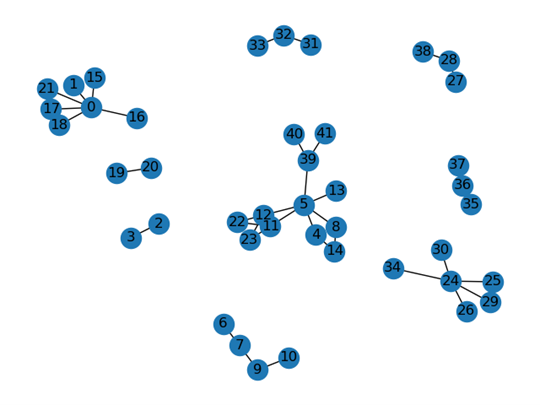
\includegraphics[width=0.75\textwidth]{all-structure}
    \bicaption{\enspace 所有流的网络拓扑结构}{\enspace Topological diagram of all flows}
    \label{fig:all-structure}

\end{figure}

与图~\ref{fig:benign-structure}~相比,图~\ref{fig:all-structure}~增加了三个节点,这些节点的 IP 地址和端口如表~\ref{tab:all-structure}~所示。

\begin{table}[t]
    \bicaption{\enspace 横向移动流中新增的节点}{\enspace Nodes added in malicious flows}
    \label{tab:all-structure}
    \centering
    \footnotesize% fontsize
    \setlength{\tabcolsep}{4pt}% column separation
    \renewcommand{\arraystretch}{1.2}%row space 
    \begin{tabular}{cccccc}
        \hline
        编号 & IP 地址 & 端口\\
        \hline
        39 & 10.16.0.45 & \geq 32768\\
        40 & 144.122.71.36 & 9001\\
        41 & 95.179.254.105 & 443\\
        \hline
    \end{tabular}
\end{table}

注意到节点 39 与节点 1 共享同一个 IP 地址,这表示它们均为 Node-RED 节点。部署 Node-RED 的负载本身无需与 API 服务器通信,但是在攻击者利用了 Node-RED 的漏洞之后,Node-RED 就会不同寻常地与 API 服务器通信,同时还与外部网络进行通信。这说明此时 Node-RED 很可能处于攻击者的 C\&C 服务器的控制之下。因此,这些节点对应的 $7$ 个流是横向移动的关键流。

最后,考虑仅包括横向移动流量的拓扑结构,如图~\ref{fig:malicious-structure}~所示。

\begin{figure}[t]
    \centering
    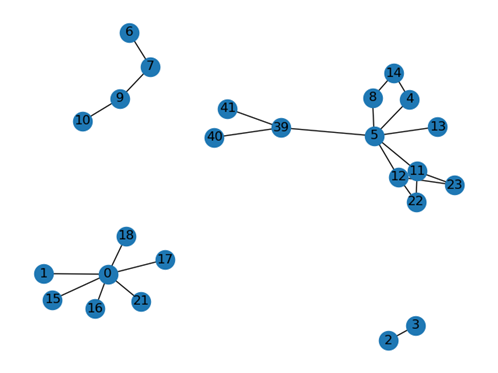
\includegraphics[width=0.75\textwidth]{malicious-structure}
    \bicaption{\enspace 横向移动流的网络拓扑结构}{\enspace Topological diagram of malicious flows}
    \label{fig:malicious-structure}

\end{figure}

从图~\ref{fig:malicious-structure}~可以看出,第(六)类通信即设备发现通信没有出现,说明设备发现通信与横向移动无关,因此可以将其从数据集中删除。

通过上述分析,本文发现,在数据集所提供的横向移动场景中,以往从未与 API 服务器和外部网络通信的 Node-RED 负载开始与 API 服务器和外部网络通信。这说明,攻击者侵入 Node-RED 负载之后,将该负载置于攻击者的 C\&C 服务器之下,并且在该负载上向 API 服务器发起非法请求,使其创建一个新的负载,以便在这个新的负载上横向移动至主机。

\section{网络流量的空间特征嵌入方法}
\label{sec:spatial}

通过拓扑分析仅能找到横向移动场景中最能体现横向移动行为的少数流量,大多数流量需要通过机器学习等方式进一步挖掘其中的信息。因此,在接下来的小节中,本文将进行特征嵌入方法的研究。

提取图中节点的空间特征并将其转换为嵌入向量,通常采用图机器学习的方法,包括 DeepWalk\citep{perozzi2014deepwalk}、Node2vec\citep{grover2016node2vec}等浅层学习方法和 GCN\citep{kipf2016semi}、GraphSAGE\citep{hamilton2017inductive}、GAT\citep{velivckovic2017graph}等深度学习方法。

DeepWalk、Node2vec 方法通过随机游走的方式在图中进行节点采样,形成若干个节点序列。若两个节点处于同一个序列中,则认为它们是相似的,它们的嵌入向量的点积应当较大;若两个节点不处于同一个序列中,则它们的嵌入向量的点积应当较小。正式的说,这两个方法的损失函数定义如公式\eqref{eq:node2vec}所示:

\begin{equation}
    \label{eq:node2vec}
    \begin{split}
        \mathcal{L} &= \sum_{u \in V} \sum_{v \in N_R(u)} - \log\frac{\exp(\mathbf{z}_u^{\mathrm{T}} \mathbf{z}_v)}{\sum_{n \in V}\exp(\mathbf{z}_u^{\mathrm{T}}\mathbf{z}_n)}.
    \end{split}
\end{equation}

公式\eqref{eq:node2vec}所示的损失函数的含义是,对于图中所有的节点$u \in V$,以随机游走的方式生成游走序列 $N_R(u)$,对于所有节点 $v \in N_R(u)$,通过 $u$ 和 $v$ 的嵌入向量的点积 $\mathbf{z}_u^{\mathrm{T}} \mathbf{z}_v$ 来计算这两个节点之间存在边的概率,并将其最大化。

为了计算概率值,需要用到 Softmax 函数,因此对于每个节点$u \in V$,需要计算所有节点$n \in V$ 与节点 $u$ 的点积,因此需要一种近似方法来降低时间复杂度。DeepWalk 和 Node2vec 采用负采样的方式近似估计损失函数,如公式\eqref{eq:node2vec-2}所示:

\begin{equation}
    \label{eq:node2vec-2}
    \begin{split}
        \mathcal{L} \approx \sum_{u \in V} (\sum_{v \in N_R(u)}\log(\sigma(\mathbf{z}_u^{\mathrm{T}} \mathbf{z}_v))+\sum_{i=1}^k \log(\sigma(-\mathbf{z}_u^{\mathrm{T}} \mathbf{z}_{n_i}))).
    \end{split}
\end{equation}

公式\eqref{eq:node2vec-2}中,$\sigma$ 表示 Sigmoid 函数。对于每个节点$u \in V$,负采样 $k$ 个节点 $n_1, \cdots, n_i, \cdots, n_k$,计算 $u$ 和 $n_i$ 的点积并求和,以替代原有的 Softmax 函数。通过将损失函数 $\mathcal{L}$ 最小化,邻近节点的嵌入向量点积得到最大化,而非邻近节点的嵌入向量点积最小化,从而学习到了图中各节点的拓扑关系。

DeepWalk 和 Node2vec 的主要区别在于随机游走的策略。在 DeepWalk 中,游走时,随机选择当前节点的邻居节点;在 Node2vec 中,游走时可选择退回上一节点、游走至上一节点的邻居节点、游走至当前节点的邻居节点的概率,让随机游走策略可以更有针对性。

然而,这类浅层学习方法有两个缺陷:

\begin{itemize}
    \item 无法学习相似但不连通或距离较远的结构。如果图中有若干个子图的拓扑结构类似但不连通或相距较远,由于随机游走无法触及,无法学习这种结构的相似性。
    \item 模型容量有限。DeepWalk 和 Node2vec 直接对节点的嵌入向量进行学习,没有经过多层神经网络,因此其容量有限,无法学习复杂的结构。
\end{itemize}

为了学习更复杂的结构,可应用 GCN、GraphSAGE、GAT 等深度学习方法。它们基于多层信息传播实现,每层信息传播将提取节点的所有邻居特征和自身节点的加权平均值,得到节点的特征向量。经过多层信息传播后得到的特征向量再输入到神经网络后可进行训练。这三种方法的信息传播细节各有不同。GCN 的信息传播模型如公式~\eqref{eq:gcn}~所示:

\begin{equation}
    \label{eq:gcn}
    \begin{split}
        \mathbf{h}_v^{(l)} &= \sigma(\mathbf{W}^{(l)} \sum_{u \in N(v)}  \frac{\mathbf{h}_u^{(l-1)}}{\left|N(v)\right|}).
    \end{split}
\end{equation}

公式~\eqref{eq:gcn}~中,$\sigma$ 代表激活函数(如 ReLU 等),$\mathbf{h}_v^{(l)}$ 表示节点 $v$ 在第 $l$ 层信息传播时的隐向量,$N(v)$ 代表 $v$ 的邻居节点的集合。该公式的含义是,每一层信息传播,将节点 $v$ 的邻居节点 $u$ 的上一层隐向量取平均值,然后经过线性变换和激活函数,得到节点 $v$ 在当前层的隐向量。

GCN 对于节点 $u$,其所有邻居都是同等重要的,实际上有可能不是。GAT 用注意力参数取代了取平均值的方法,其信息传播模型如公式~\eqref{eq:gat}~所示:

\begin{equation}
    \label{eq:gat}
    \begin{split}
        \mathbf{h}_v^{(l)} &= \sigma(\mathbf{W}^{(l)} \sum_{u \in N(v)} \alpha_{vu} \mathbf{h}_u^{(l-1)}).
    \end{split}
\end{equation}

然而,GCN 和 GAT 在进行信息传播时,只考虑邻居节点的上一层隐向量,而忽略了节点本身的上一层隐向量。GraphSAGE 把节点本身的上一层隐向量也纳入考虑范围,其信息传播模型如公式~\eqref{eq:sage}~所示:

\begin{equation}
    \label{eq:sage}
    \begin{split}
        \mathbf{h}_v^{(l)} &= \sigma(\mathbf{W}^{(l)}  \mathrm{concatenate}(\mathbf{h}_v^{(l-1)},\sum_{u \in N(v)}  \frac{\mathbf{h}_u^{(l-1)}}{\left|N(v)\right|})).
    \end{split}
\end{equation}

为了训练这些图深度学习模型并得到最终的嵌入向量,还需要定义损失函数。本文借用 DeepWalk 和 Node2vec 的方法定义损失函数,如公式\eqref{eq:node2vec-2}所示,其中的 $\mathbf{z}_u$ 代表节点 $u$ 经过所有层信息传播模型后得到的隐向量,该向量作为节点 $u$ 的嵌入向量。经过多轮训练后,得到最终的图深度学习模型和各节点的嵌入向量,供后续模型使用。具体选用的模型将在第~\ref{sec:experiment-spatial}~节中讨论。

\section{网络流量的时间特征嵌入方法}
\label{sec:temporal}

处理时间序列数据通常使用循环神经网络,常用的方法包括 GRU 和 LSTM。GRU 和 LSTM 可以处理时序数据,通过门控单元,避免了梯度消失问题,可以学习到时间上间隔较远的两条记录之间的依赖关系。

GRU 有两个门控单元,分别是重置门和更新门。模型定义如公式\eqref{eq:gru}所示:

\begin{equation}
    \label{eq:gru}
    \begin{split}
        \Tilde{\mathbf{c}}^{(t)} &= \tanh{(\mathbf{W}_c \mathrm{concatenate}(\mathbf{\tau}_r \ast \mathbf{c}^{(t-1)},\mathbf{x}^{(t)}) + b_c)} ,\\
        \mathbf{\tau}_u &= \sigma{(\mathbf{W}_u \mathrm{concatenate}(\mathbf{c}^{(t-1)},\mathbf{x}^{(t)}) + b_u)} ,\\
        \mathbf{\tau}_r &= \sigma{(\mathbf{W}_r \mathrm{concatenate}(\mathbf{c}^{(t-1)},\mathbf{x}^{(t)}) + b_r)} ,\\
        \mathbf{c}^{(t)} &= \mathbf{\tau}_u \ast \Tilde{\mathbf{c}}^{(t)} + (1-\mathbf{\tau}_u) \ast \mathbf{c}^{(t-1)} ,\\
        \mathbf{a}^{(t)} &= \mathbf{c}^{(t)}.
    \end{split}
\end{equation}

在公式\eqref{eq:gru}中,$\mathbf{x}^{(t)}$ 表示当前时刻的输入,$\mathbf{a}^{(t)}$ 代表当前时刻的输出,$\sigma$ 代表激活函数。$\mathbf{c}^{(t)}$ 表示当前时刻的隐藏状态,它由当前时刻的候选隐藏状态 $\Tilde{\mathbf{c}}^{(t)}$ 和上一时刻的隐藏状态 $\mathbf{c}^{(t-1)}$ 的加权平均确定,而更新门 $\mathbf{\tau}_u$ 则确定前者的权重。重置门 $\mathbf{\tau}_r$ 则用于控制对过去的信息的遗忘程度,以计算当前时刻的候选隐藏状态 $\Tilde{\mathbf{c}}^{(t)}$。$\mathbf{W}_i, b_i (i \in {u, r})$ 是待学习的参数。

LSTM 则有三个门控单元,分别是遗忘门、更新门和输出门。模型定义如公式\eqref{eq:lstm}所示:

\begin{equation}
    \label{eq:lstm}
    \begin{split}
        \Tilde{\mathbf{c}}^{(t)} &= \tanh{(\mathbf{W}_c \mathrm{concatenate}(\mathbf{a}^{(t-1)},\mathbf{x}^{(t)}) + b_c)} ,\\
        \mathbf{\tau}_u &= \sigma{(\mathbf{W}_u \mathrm{concatenate}(\mathbf{a}^{(t-1)},\mathbf{x}^{(t)}) + b_u)} ,\\
        \mathbf{\tau}_f &= \sigma{(\mathbf{W}_f \mathrm{concatenate}(\mathbf{a}^{(t-1)},\mathbf{x}^{(t)}) + b_f)} ,\\
        \mathbf{\tau}_o &= \sigma{(\mathbf{W}_o \mathrm{concatenate}(\mathbf{a}^{(t-1)},\mathbf{x}^{(t)}) + b_o)} ,\\
        \mathbf{c}^{(t)} &= \mathbf{\tau}_u \ast \Tilde{\mathbf{c}}^{(t)} + \mathbf{\tau}_f \ast \mathbf{c}^{(t-1)} ,\\
        \mathbf{a}^{(t)} &= \mathbf{\tau}_o \ast \mathbf{c}^{(t)}.
    \end{split}
\end{equation}

在公式\eqref{eq:lstm}中,$\mathbf{x}^{(t)}$ 表示当前时刻的输入,$\mathbf{a}^{(t)}$ 代表当前时刻的输出,$\sigma$ 代表激活函数。$\mathbf{c}^{(t)}$ 表示当前时刻的隐藏状态,它由当前时刻的候选隐藏状态 $\Tilde{\mathbf{c}}^{(t)}$ 和上一时刻的隐藏状态 $\mathbf{c}^{(t-1)}$ 的加权平均确定,而遗忘门 $\mathbf{\tau}_f$ 和更新门 $\mathbf{\tau}_u$ 则确定它们的权重。输出门 $\mathbf{\tau}_o$ 则用于对隐藏状态再作一个线性变换,得到当前时刻的输出。$\mathbf{W}_i, b_i (i \in {u, f, o})$ 是待学习的参数。

GRU 和 LSTM 均支持多层堆叠。堆叠时,下层 GRU 或 LSTM 的输出 $\mathbf{a}^{(t)\left[l-1\right]}$ 作为上层 GRU 或 LSTM 的输入 $\mathbf{x}^{(t)\left[l\right]}$。多层堆叠可以捕捉更复杂的依赖关系。

由于 GRU 的门控单元较少,LSTM 的门控单元更多,因此 LSTM 有更强的表达能力,可以处理更长序列的数据。因此,本文将选用 LSTM 作为网络流量的时间特征转换方法。此外,由于网络流量的变化频繁多样,因此适合采用多层堆叠的方法,本文将采用三层堆叠的 LSTM。将网络流量的子序列输入到三层 LSTM 之后,取 LSTM 最后一个时刻的输出,供后续模型使用。

\section{实验验证}

本节将对网络流量的空间和时间特征嵌入方法进行验证。

\subsection{空间特征嵌入方法验证}
\label{sec:experiment-spatial}

本文将通过公式\eqref{eq:node2vec-2}所示的损失函数,对 DeepWalk、Node2vec、GCN、GraphSAGE 和 GAT 的损失函数值随训练轮数的下降情况进行对比。

对于 DeepWalk 和 Node2vec,本文对比了它们在不同的超参数下的实验结果,具体超参数如表~\ref{tab:hyperparameters-deep-walk-node2vec}~所示。对于每个模型,对比了 Local 和 Global 两种方法,Local 方法的随机游走长度和窗口长度比 Global 方法更短,Local 方法更针对相邻节点之间进行损失函数估计,而 Global 方法则针对节点所在的更大的连通分量区域进行损失函数估计。

\begin{table}[!htbp]
    \bicaption{\enspace DeepWalk 和 Node2vec 的实验超参数设置}{\enspace Hyperparameters of DeepWalk and Node2vec}
    \label{tab:hyperparameters-deep-walk-node2vec}
    \centering
    \footnotesize% fontsize
    \setlength{\tabcolsep}{4pt}% column separation
    \renewcommand{\arraystretch}{1.2}%row space 
    \begin{tabular}{ccccccc}
        \hline
        名称 & 模型 & 嵌入向量维度 & 随机游走长度 & 窗口长度 & 每节点随机游走数\\
        \hline
        Node2vec-Local & Node2vec & 36 & 4 & 2 & 20\\
        Node2vec-Global & Node2vec & 36 & 20 & 10 & 20\\
        DeepWalk-Local & DeepWalk & 36 & 4 & 2 & 20\\
        DeepWalk-Global & DeepWalk & 36 & 20 & 10 & 20\\
        \hline
    \end{tabular}
\end{table}

其损失函数值随训练轮数的下降情况如图~\ref{fig:deep-walk-node2vec}~所示。可以看出,在图中所示的学习率中,0.2 是两种模型最优的学习率;此外,与 Local 方法相比,相应的 Global 方法更稳定。这说明,对于容器化集群网络流量构成的图,从更加宏观、全局的角度可以更稳定地学习图的结构。

\begin{figure}[!htbp]
    \centering
    \begin{subfigure}[b]{0.48\textwidth}
      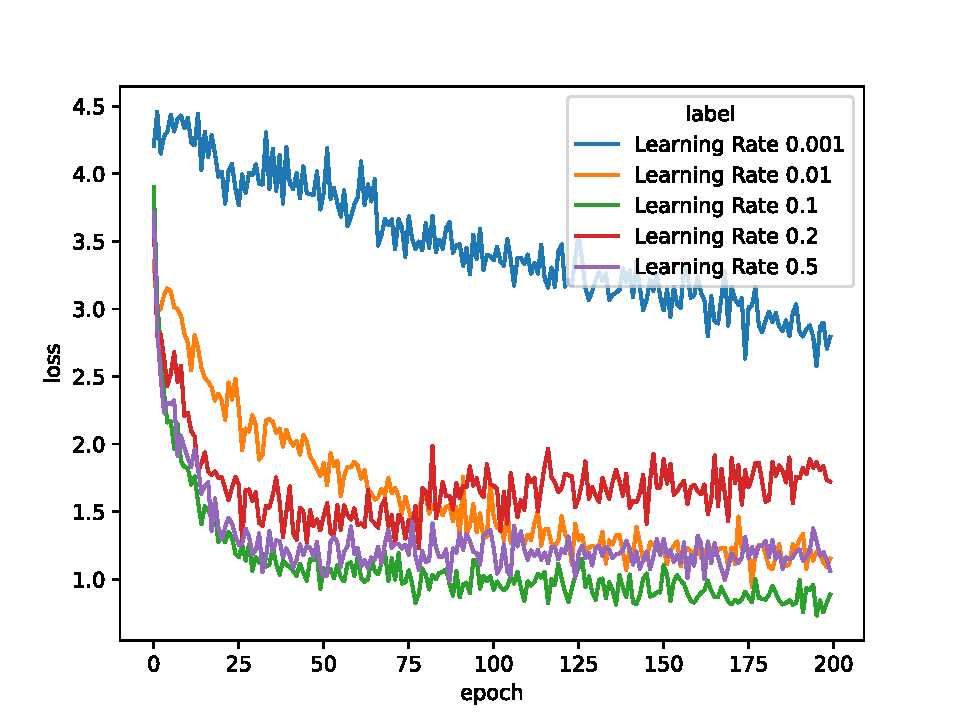
\includegraphics[width=\textwidth]{Node2vec-local}
      \caption{Node2vec-Local}
    \end{subfigure}
    ~
    \begin{subfigure}[b]{0.48\textwidth}
      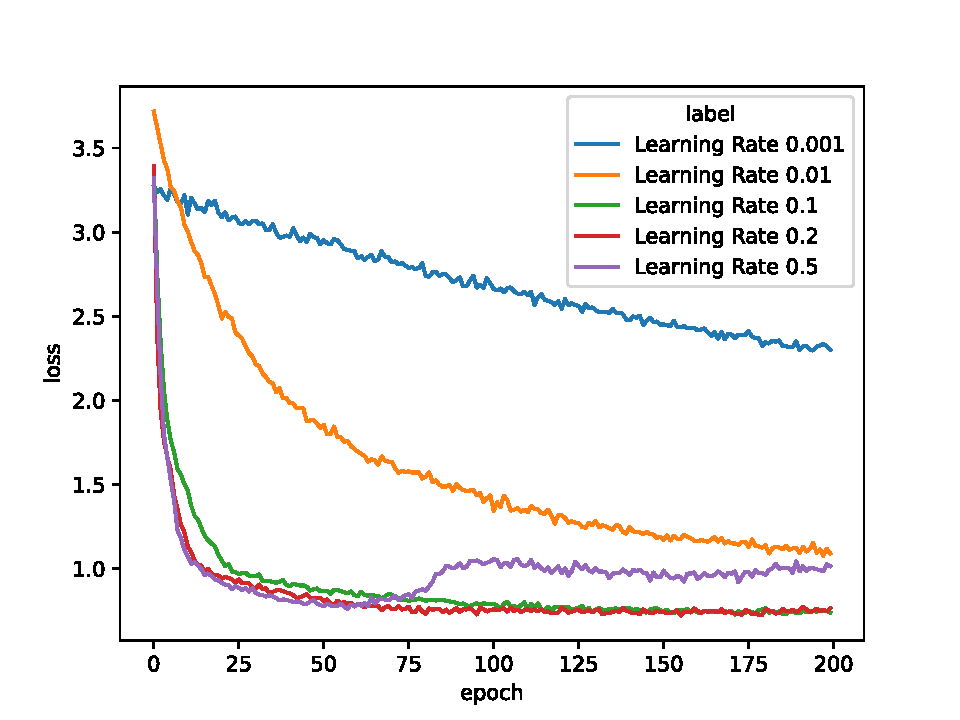
\includegraphics[width=\textwidth]{Node2vec-global}
      \caption{Node2vec-Global}
    \end{subfigure}
    \\
    \begin{subfigure}[b]{0.48\textwidth}
      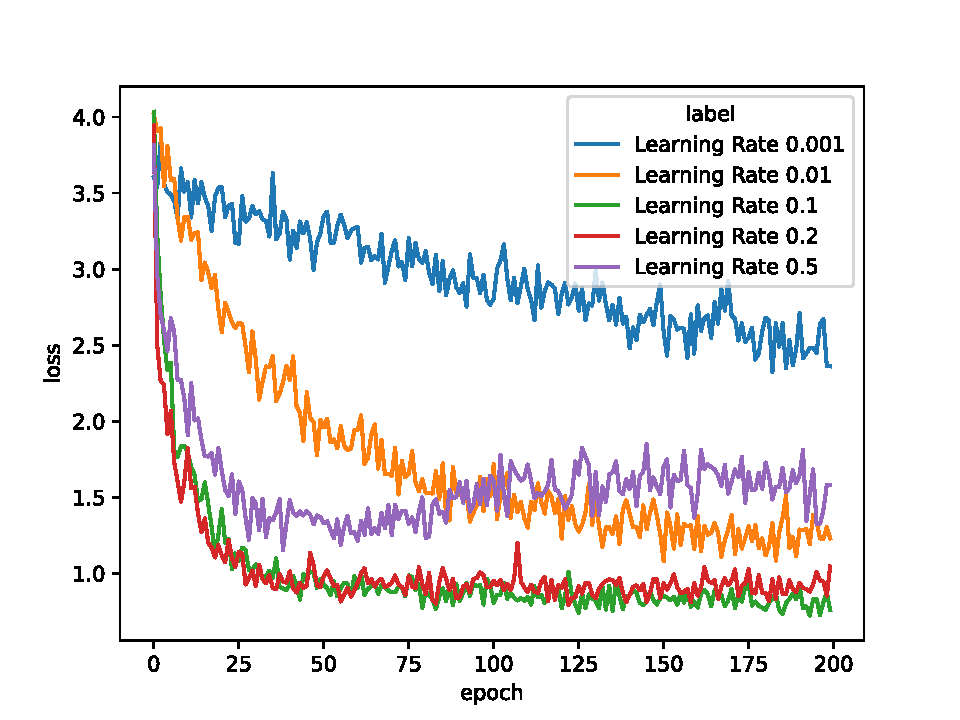
\includegraphics[width=\textwidth]{DeepWalk-local}
      \caption{DeepWalk-Local}
    \end{subfigure}
    ~
    \begin{subfigure}[b]{0.48\textwidth}
      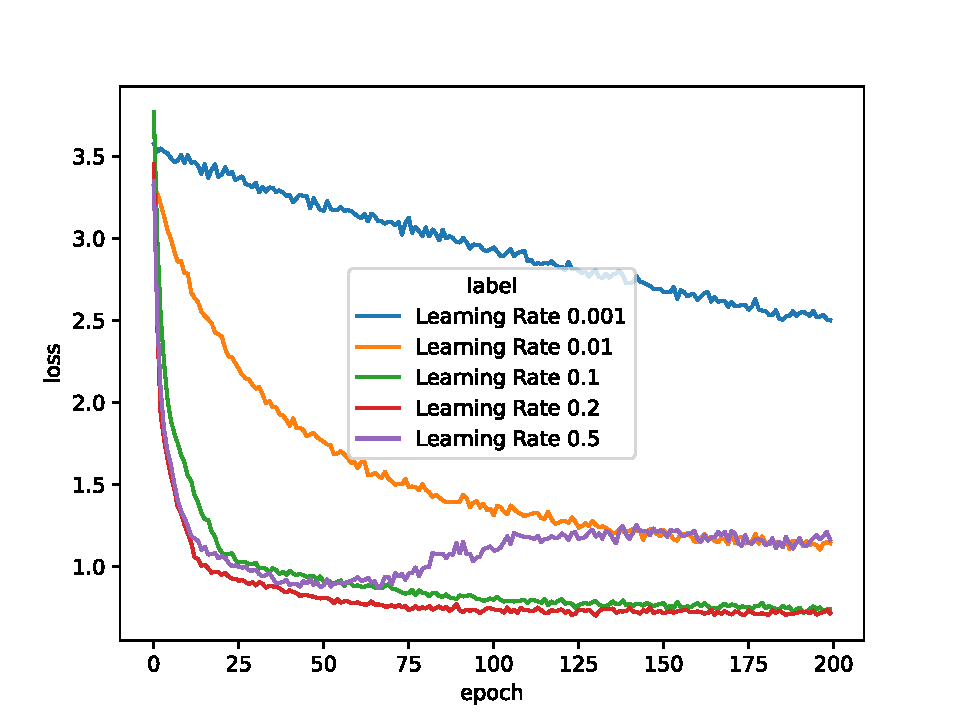
\includegraphics[width=\textwidth]{DeepWalk-global}
      \caption{DeepWalk-Global}
    \end{subfigure}
    \bicaption{\enspace DeepWalk 和 Node2vec 损失函数值与训练轮数曲线图}{\enspace Plots of DeepWalk and Node2vec's loss function values with epoches}
    \label{fig:deep-walk-node2vec}
\end{figure}

对于 GCN、GraphSAGE 和 GAT,本文采用了两个图卷积层,第一个图卷积层采用了 ReLU 激活函数,并有概率为 0.1 的失活(Dropout)层,以避免过拟合;第二个图卷积层采用了 TanH 激活函数。它们的超参数如表~\ref{tab:hyperparameters-gnns}~所示。

\begin{table}[!htbp]
    \bicaption{\enspace GCN、GraphSAGE 和 GAT 的实验超参数设置}{\enspace Hyperparameters of GCN, GraphSAGE and GAT}
    \label{tab:hyperparameters-gnns}
    \centering
    \footnotesize% fontsize
    \setlength{\tabcolsep}{4pt}% column separation
    \renewcommand{\arraystretch}{1.2}%row space 
    \begin{tabular}{ccccccc}
        \hline
        名称 & 模型 & 输入维度 & 隐向量维度 & 输出维度\\
        \hline
        GCN & GCN & 36 & 36 & 36\\
        GraphSAGE & GraphSAGE & 36 & 36 & 36\\
        GAT & GAT & 36 & 36 & 36\\
        \hline
    \end{tabular}
\end{table}

这些模型损失函数值随训练轮数的下降情况如图~\ref{fig:gnns}~所示。可以看出,在图中所示的学习率中,0.01 是三种模型最优的学习率;此外,三种深度图神经网络模型无需只需要很少的迭代就能到达收敛状态。

\begin{figure}[!htbp]
    \centering
    \begin{subfigure}[b]{0.48\textwidth}
      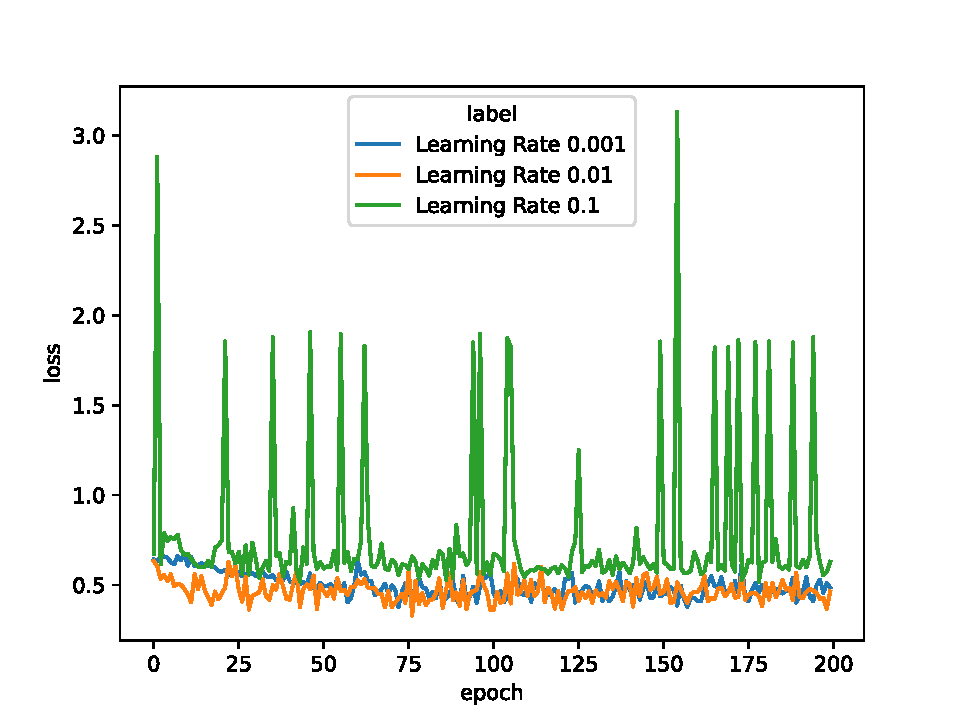
\includegraphics[width=\textwidth]{GCN}
      \caption{GCN}
    \end{subfigure}
    ~
    \begin{subfigure}[b]{0.48\textwidth}
      \includegraphics[width=\textwidth]{SAGE}
      \caption{GraphSAGE}
    \end{subfigure}
    \\
    \begin{subfigure}[b]{0.48\textwidth}
      \includegraphics[width=\textwidth]{GAT}
      \caption{GAT}
    \end{subfigure}
    \bicaption{\enspace GCN、GraphSAGE 和 GAT 损失函数值与训练轮数曲线图}{\enspace Plots of GCN, GraphSAGE and GAT's loss function values with epoches}
    \label{fig:gnns}
\end{figure}

最后,取上述五个模型的最佳学习率进行对比,其曲线图如图~\ref{fig:graph-plots}~所示。

\begin{figure}[!htbp]
    \centering
    \includegraphics[width=0.48\textwidth]{ALL}
    \bicaption{\enspace 五个图机器学习模型损失函数值与训练轮数曲线图}{\enspace Plots of Five Graph Learning Models' loss function values with epoches}
    \label{fig:graph-plots}
\end{figure}

从图~\ref{fig:graph-plots}~可以看出,在这些机器学习模型中,基于深度学习的模型比基于随机游走的浅层模型收敛更快,这是因为深度学习模型具有更大的容量,有更强的表达能力。在基于深度学习的模型中,三个模型的损失函数值差别不大,但 GCN 模型最为稳定。因此,本文将采用 GCN 模型作为空间特征嵌入方法进行后续的横向移动检测方法研究。

\subsection{时间特征嵌入方法验证}

对于循环神经网络模型 GRU 和 LSTM,本文采用了预测的方式来比较它们的性能,即先将 Kubernetes-dataset 中的良性流量按时间顺序排列后,划分为一定长度的子序列,然后输入至循环神经网络模型中,由循环神经网络模型输出下一时刻的流量预测值,最后取预测值和实际值的欧几里得距离作为模型的评估指标。本文所采用的超参数设置如表~\ref{tab:hyperparameters-rnns}~所示。

\begin{table}[!htbp]
    \bicaption{\enspace GRU 和 LSTM 的实验超参数设置}{\enspace Hyperparameters of GRU and LSTM}
    \label{tab:hyperparameters-rnns}
    \centering
    \footnotesize% fontsize
    \setlength{\tabcolsep}{4pt}% column separation
    \renewcommand{\arraystretch}{1.2}%row space 
    \begin{tabular}{ccccccc}
        \hline
        名称 & 模型 & 层数 & 隐向量维度 & 学习率\\
        \hline
        GRU-1 & GRU & 1 & 同输入流量特征维度 & 0.01\\
        GRU-3 & GRU & 3 & 同输入流量特征维度 & 0.01\\
        LSTM-1 & LSTM & 1 & 同输入流量特征维度 & 0.01\\
        LSTM-3 & LSTM & 3 & 同输入流量特征维度 & 0.01\\
        \hline
    \end{tabular}
\end{table}

其损失函数值随训练轮数的下降情况如图~\ref{fig:rnn-plot}~所示。在这些循环神经网络模型中,三层堆叠的模型比单层堆叠的收敛速度更快,损失函数值更低;与 GRU 相比,LSTM 的预测值更准确,收敛速度也占优势。

\begin{figure}[!htbp]
    \centering
    \includegraphics[width=0.48\textwidth]{RNN}
    \bicaption{\enspace GRU 和 LSTM 损失函数值与训练轮数曲线图}{\enspace Plots of GRU and LSTM's loss function values with epoches}
    \label{fig:rnn-plot}
\end{figure}

为了进一步验证四种模型的效果,本文将良性流量的子序列划分为训练集和测试集,其中训练集占比 70\%,测试集占比 30\%。四种模型在测试集上的均方误差如表~\ref{tab:result-rnns}~所示。采用三层 LSTM 的均方误差最低,因此其效果最好。这说明,容量更大的模型具有更强的表达能力。本文将采用三层 LSTM 模型作为时间特征嵌入方法进行后续的横向移动检测模型研究。

\begin{table}[!htbp]
    \bicaption{\enspace GRU 和 LSTM 在测试集上的均方误差结果}{\enspace MSE loss of GRU and LSTM on the test set}
    \label{tab:result-rnns}
    \centering
    \footnotesize% fontsize
    \setlength{\tabcolsep}{4pt}% column separation
    \renewcommand{\arraystretch}{1.2}%row space 
    \begin{tabular}{ccccccc}
        \hline
        名称 & 均方误差\\
        \hline
        GRU-1 & 0.37442\\
        GRU-3 & 0.32283\\
        LSTM-1 & 0.29323\\
        LSTM-3 & 0.28088\\
        \hline
    \end{tabular}
\end{table}

\section{本章小结}

本节首先通过可视化的方式分析容器化集群中网络流量的拓扑结构,对各类通信模式进行了分类,发现了横向移动的关键流。此类流表示一个负载正在攻击者的 C\&C 服务器的控制之下,与 API 服务器进行通信,反映了横向移动攻击的行为。

然而,通过拓扑分析仅能识别出少量的横向移动流量,大部分横向移动流量未能检出。因此,还需要通过机器学习的方法进行识别。本章分析了图神经网络和循环神经网络的多种模型,总结其优缺点,最终选用 GCN 和 LSTM 分别作为时间和空间特征嵌入方法,分别得到各节点的嵌入向量和时间特征向量,供后续模型使用。

}
% \chapter{容器化环境中的横向移动检测模型}{
{
\let\cleardoublepage\relax
}



}
% \chapter{总结与展望}{
{
\let\cleardoublepage\relax
}
}
\chapter{基于 Transformer 的两阶段横向移动检测方法}{
{
\let\cleardoublepage\relax
}

根据本文第~\ref{chap:analyze}~章和第~\ref{chap:embedding}~章的分析,攻击者发起横向移动攻击之后,将使得一部分横向移动流量在批量传输特征、数据包长度特征等的值超出了良性流量相应的值域,并且使网络的拓扑结构发生更改,这反映了攻击者利用被攻破的负载与集群的 API 服务器进行非法通信等行为。此外,还有大多数横向移动流量仍然十分隐蔽,不能通过特征分析和拓扑分析直接进行分类。

因此,本文将分别针对这两类横向移动流量进行研究,并提出基于 Transformer 的两阶段横向移动检测方法。该方法应能:

\begin{itemize}
    \item 检出关键横向移动流量,这些横向移动流量体现出横向移动的关键行为;
    \item 对于大多数横向移动流量,应在误报率较低的水平上尽可能提高检测率,AUC 分数达到 95\% 以上,优于其他现有的模型。
\end{itemize}

本章将提出基于 Transformer 的两阶段横向移动检测方法。在第一阶段,基于最值和拓扑的横向移动检测方法负责检测关键的横向移动流量;在第二阶段,基于 Transformer 的横向移动检测模型 LMDCE 检测大多数横向移动流量,由空间特征嵌入模块、时间特征嵌入模块、编码器—解码器模块和两阶段预测机制构成,以提高模型的性能。本文通过实验,验证了方法的有效性,并且其性能高于已有的方法。

\section{问题定义}

本文考虑的横向移动检测是一个自监督的问题。给定时间连续的两个流量序列
\begin{equation}
    \label{eq:definition}
    \begin{split}
        \tau_1 &= \left \langle X_1, X_2, \cdots, X_t \right \rangle ,\\
        \tau_2 &= \left \langle X_{t+1}, X_{t+2}, \cdots, X_T \right \rangle ,
    \end{split}
\end{equation}
在假设 $\tau_1$ 为良性流量序列的情况下,需对未知序列 $\tau_2$ 中的每个流量 $X_i$ 进行二分类,分类结果为该流量是良性流量,或该流量是横向移动流量。

其中,每个流量 $X_i$ 由源节点 $s_i$、目的节点 $d_i$ 和流量特征 $\mathbf{x}_i$ 组成。

\section{总体流程}

方法的总体流程如图~\ref{fig:total-model}~所示。

\begin{figure}[t]
    \centering
    \includegraphics[width=0.75\textwidth]{total-model}
    \bicaption{\enspace 基于 Transformer 的两阶段横向移动检测方法总体流程}{\enspace The overall workflow of the lateral movement detection method based on Transformer}
    \label{fig:total-model}

\end{figure}

流量按时间顺序逐个输入。按照本研究的目标,方法将由两阶段构成。

为了检出关键的横向移动流量,方法首先将根据最值和拓扑对流量进行检测,未能通过检测(即被识别为横向移动)的流量将发出告警;通过检测的大部分流量,再由基于 Transformer 的横向移动检测模型进行检测,未能通过检测的流量将发出告警,通过检测的流量视为正常流量。

将方法分为两个阶段进行设计有两个好处:

\begin{itemize}
    \item 提高了可解释性。基于最值和拓扑的检测方法具有很强的可解释性,该方法可以明确指出横向移动流量的哪些特征超出了正常范围,或它导致网络流量拓扑发生了哪些改变;而基于 Transformer 等深度学习的模型具有不可解释性\citep{SAEED2023110273}。
    \item 提高了横向移动流量的检测率。基于 Transformer 的横向移动检测模型进行检测可以检出绝大多数的横向移动流量,是高检测率的支柱;而基于最值和拓扑的检测方法可以进一步检出前述模型尚不能检出的横向移动流量,是该模型的补充,可进一步提高检测率。
\end{itemize}

\section{第一阶段:基于最值和拓扑的横向移动检测}

本节将利用第~\ref{sec:extreme}~节和第~\ref{sec:topology}~节的分析结果,对横向移动流量进行检测。

\subsection{基于最值的横向移动流量检测}

根据第~\ref{sec:extreme}~节的最值分析,横向移动将改变容器化集群中的网络流量模式,使连续活跃时长最大值等特征的值超过了良性流量的相应值。因此,本文提出了基于最值的横向移动流量检测方法。该方法分为两个阶段进行:

\begin{itemize}
    \item 训练阶段。在该阶段,读入网络流量,更新网络流量特征的最值。
    \item 检测阶段。在该阶段,读入网络流量,并判断其各项特征是否超出了最值,超出的判定为横向移动。
\end{itemize}

该方法使用的特征包括前向数据包长度最大值、前向每 bulk 传输字节数、前向每 bulk 传输数据包数、前向 bulk 速率、连续活跃时长最大值。这些特征的有关分析见第~\ref{sec:extreme}~节。

方法的伪代码如图~\ref{fig:detect-code}~所示。

\begin{figure}[t]
    \centering
    \begin{subfigure}[b]{1.0\textwidth}
        \hrulefill
        \begin{algorithmic}[1]
            \Require $\tau_1$, FeatureList
            \Ensure MinMap, MaxMap
            \Function {TrainMap}{$\tau_1$, FeatureList}
                \State MinMap $\gets \emptyset$, MaxMap $\gets \emptyset$
                \For{$X$ \textbf{in} $\tau_1$}
                    \For{Feature \textbf{in} FeatureList}
                        \State MinMap[Feature] $\gets $ Min (MinMap[Feature], $X$[Feature])
                        \State MaxMap[Feature] $\gets $ Max (MinMap[Feature], $X$[Feature])
                    \EndFor
                \EndFor
            \EndFunction
            \end{algorithmic}
        \hrulefill
        \caption{训练阶段}
    \end{subfigure}
    \\
    \begin{subfigure}[b]{1.0\textwidth}
        \hrulefill
            \begin{algorithmic}[1]
            \Require $\tau_2$, FeatureList, MinMap, MaxMap
            \Ensure Alerts
            \Function{TestFlow1}{$\tau_2$, FeatureList, MinMap, MaxMap}
                \For{$X$ \textbf{in} $\tau_2$}
                    \For{Feature \textbf{in} FeatureList}
                        \If{$X$[Feature] $\notin$ [MinMap[Feature],MaxMap[Feature]]}
                            \State \textbf{alert} $X$
                        \EndIf
                    \EndFor
                \EndFor
            \EndFunction
            \end{algorithmic}
        \hrulefill
        \caption{检测阶段}
    \end{subfigure}
    \bicaption{\enspace 基于最值的横向移动流检测伪代码}{\enspace Pseudocode of detecting lateral movements based on min and max values}
    \label{fig:detect-code}
\end{figure}

\subsection{基于拓扑的横向移动流量检测}
\label{sec:detect-on-topology}

根据第~\ref{sec:topology}~节的拓扑分析,横向移动将改变容器化集群中的拓扑结构。本文检测以下拓扑结构的变更:

\begin{itemize}
    \item 负载节点增加;
    \item 与 API 服务器通信的节点增加,或从未与 API 服务器通信的节点开始通信;
    \item 从未访问外部网络的负载节点开始访问外部网络。
\end{itemize}

方法的伪代码如图~\ref{fig:detect-topology-code}~所示。

\begin{figure}[t]
    \centering
    \begin{subfigure}[b]{1.0\textwidth}
        \hrulefill
        \begin{algorithmic}[1]
            \Require $\tau_1$, ApiServer
            \Ensure PodSet, ApiSet, PodExternalSet
            \Function {TrainSet}{$\tau_1$, ApiServer}
                \State PodSet $\gets \emptyset$, ApiSet $\gets \emptyset$, PodExternalSet $\gets \emptyset$
                \For{$X$ \textbf{in} $\tau_1$}
                    \State $s, d \gets X$
                    \State Append $s$ to PodSet if $s$ is a Pod
                    \State Append $d$ to PodSet if $d$ is a Pod
                    \State Append $s$ to ApiSet if $d$ equals ApiServer
                    \State Append $d$ to ApiSet if $s$ equals ApiServer
                    \State Append $s$ to PodExternalSet if $s$ is a Pod and $d$ is an external node
                    \State Append $d$ to PodExternalSet if $d$ is a Pod and $s$ is an external node
                \EndFor
            \EndFunction
            \end{algorithmic}
        \hrulefill
        \caption{训练阶段}
    \end{subfigure}
    \\
    \begin{subfigure}[b]{1.0\textwidth}
        \hrulefill
            \begin{algorithmic}[1]
            \Require $\tau_2$, ApiServer, PodSet, ApiSet, PodExternalSet
            \Ensure Alerts
            \Function{TestFlow2}{$\tau_2$, ApiServer, PodSet, ApiSet, PodExternalSet}
                \For{$X$ \textbf{in} $\tau_2$}
                    \State $s, d \gets X$
                    \State malicious $\gets 0$
                    \State Set malicious to 1 if $s \notin$ PodSet and $s$ is a Pod
                    \State Set malicious to 1 if $d \notin$ PodSet and $d$ is a Pod
                    \State Set malicious to 1 if $s \notin$ ApiSet and $d$ equals ApiServer
                    \State Set malicious to 1 if $d \notin$ ApiSet and $s$ equals ApiServer
                    \State Set malicious to 1 if $s \notin$ PodExternalSet and $s$ is a Pod and $d$ is an external node
                    \State Set malicious to 1 if $d \notin$ PodExternalSet and $d$ is a Pod and $s$ is an external node
                    \If{malicious $= 1$}
                        \State \textbf{alert} $X$
                    \EndIf
                \EndFor
            \EndFunction
            \end{algorithmic}
        \hrulefill
        \caption{检测阶段}
    \end{subfigure}
    \bicaption{\enspace 基于拓扑结构的横向移动流检测伪代码}{\enspace Pseudocode of detecting lateral movements based on topology}
    \label{fig:detect-topology-code}
\end{figure}

\section{第二阶段:LMDCE,基于 Transformer 的横向移动检测模型}

对于大部分横向移动流量,其检测的难点在于:它们隐蔽在正常流量之间,无法直接利用它们的特征判别出来。特别是,经过了基于最值和拓扑的检测之后,横向移动流量就更加隐蔽了。尽管本文已经提取了这些流量的空间嵌入向量和时间嵌入向量,但是,还需要有效的深度学习模型才能进行检测。

因此,本文提出了基于 Transformer 的横向移动检测模型,并称其为 LMDCE(Lateral Movement Detection in Containerized Environments)。LMDCE 的结构如图~\ref{fig:model}~所示。

\begin{figure}[t]
    \centering
    \includegraphics[width=1.00\textwidth]{model}
    \bicaption{\enspace LMDCE 模型结构}{\enspace The architecutre of LMDCE}
    \label{fig:model}

\end{figure}

LMDCE 是基于预测的横向移动检测模型。LMDCE 分为空间特征嵌入模块、时间特征嵌入模块、编码器—解码器模块和两步预测机制。

\subsection{空间特征嵌入模块}

LMDCE 采用 GCN 作为空间特征嵌入方法,如第~\ref{sec:spatial}~节所述。

考虑到在基于拓扑的横向移动流量检测中,包含有新负载的流量已经被识别为横向移动流量,因此,在 LMDCE 中,可以将网络流量拓扑图视为静态的。因此,本模块独立进行训练,输入训练流量序列 $\tau_1$ 后,经过训练,为 $\tau_1$ 的每个节点生成嵌入向量。

在测试流量序列 $\tau_2$ 中,可能包含 $\tau_1$ 中所没有的新节点,因此需要考虑这些节点的嵌入向量。根据容器化集群网络结构(图~\ref{fig:networking}),新节点可能是新的服务、新的负载、新的主机或新的外部节点。新的主机需要容器化集群的管理员来配置,因此由攻击者创建的可能性较低,不纳入 LMDCE 的考虑范围。新的服务依赖于新的负载,而新的负载在第~\ref{sec:detect-on-topology}~节就已被筛除,因此不纳入 LMDCE 的考虑范围。所以,在 $\tau_2$ 中包含的节点只可能是新的外部节点。对于新的外部节点,本模块随机生成向量作为该节点的嵌入向量。

\subsection{时间特征嵌入模块}
\label{sec:temporal-module}

LMDCE 采用三层 LSTM 作为时间特征嵌入方法,如第~\ref{sec:temporal}~节所述。

在 LMDCE 中,时间特征嵌入模块的输出为时间特征嵌入向量,作为后续编码器—解码器模块的输入,用于自注意力机制。因此,本模块将与编码器—解码器模块一起进行训练和测试。

在自注意力机制中,时间特征嵌入向量的作用是让模型根据当前时间的特征,从编码器输出的隐向量中获取与当前特征最有关联性的信息,有助于模型生成预测,降低良性流量的预测误差,从而降低模型的误报率。

\subsection{编码器—解码器模块}

LMDCE 的编码器—解码器受 Transformer\citep{vaswani2017attention} 启发进行设计。它接收一个长度为 $n$ 的流量窗口 $W=\left<X_{t-n},\cdots,X_{t-1}\right>$ 和时间特征嵌入向量,输出该窗口下一个时刻的流量预测 $\hat{X}_t$。其中流量 $X_i$ 由源节点 $s_i$ 所对应的嵌入向量 $\mathbf{s}_i$、目的节点 $d_i$ 所对应的嵌入向量 $\mathbf{d}_i$ 和流量特征 $\mathbf{x}_i$ 连接而成。

流量窗口经过位置编码后输入到编码器中。通过多头注意力机制,编码器可以并行地处理流量窗口,计算流量之间的相关性和依赖关系\citep{vaswani2017attention}。通过前馈网络,编码器可以学习到更复杂的语义关系。最终,编码器生成隐向量。

隐向量和时间特征嵌入向量输入至解码器中。通过多头注意力机制,编码器可以并行地检索时间特征嵌入向量与流量窗口之间的相关性。编码器将根据时间特征嵌入向量,查询流量窗口中最相关的流量,随后经过输出层,得到当前流量窗口的预测。

\subsection{两步预测机制}

LMDCE 的两步预测机制受 USAD\citep{audibert2020usad}、TranAD\citep{tuli2022tranad} 的启发进行设计,但进行了改进,以进一步提高性能。

由于生成对抗网络和对抗训练机制存在不稳定性和收敛困难等问题\citep{darban2022deep,kodali2017convergence},通常不适合在线使用。因此,本文没有像以往的工作\citep{audibert2020usad, tuli2022tranad, li2019mad}那样采用对抗训练的方式,而是采用一种两步预测的方式来提升模型的性能。LMDCE 使用了一个编码器和两个解码器用于两步预测。

在第一步,模型使用编码器和第一个解码器预测流量 $X_t$,预测值为 $O_1$。随后,LMDCE 将计算 $O_1$ 与 $X_t$ 的误差,得到误差向量 $E$。

在第二步,将 $E$ 与流量窗口 $W$ 连接,再次输入至 LMDCE 的编码器中。此时,编码器中与误差向量相接的神经元将会激活,自注意力机制将更关注第一次预测中存在误差的部分。LMDCE 使用同一个编码器和第二个解码器预测流量 $X_t$,预测值为 $O_2$。

通过将误差向量重新输入至模型中,LMDCE 对良性流量的预测更准确,有助于降低误报率。

\subsection{LMDCE 的训练过程}

LMDCE 的时间特征嵌入模块单独进行训练,训练过程参见第~\ref{sec:temporal-module}~节。训练完成后,得到网络流量各节点对应的嵌入向量。

对于训练流量序列 $\tau_1$ 中的每个流量 $X_t$,取 $X_t$ 之前(不含)长度为 $n$ 的流量序列作为流量窗口 $W_t$。模型接收 $W_t$ 作为输入,输出两个预测值 $O_{1,t}$ 和 $O_{2,t}$。本文分别计算这两个预测值与实际值 $X_t$ 的误差
\begin{equation}
    \label{eq:loss}
    \begin{split}
        l_{1,t} &= \left\Vert O_1 - X_t \right\Vert,\\
        l_{2,t} &= \left\Vert O_2 - X_t \right\Vert,
    \end{split}
\end{equation}
随后,将误差加权平均,得到
\begin{equation}
    \label{eq:total-loss}
    \begin{split}
        l_t &= \epsilon l_{1,t} + (1-\epsilon)l_{2,t} ,
    \end{split}
\end{equation}
其中 $\epsilon$ 随着训练的迭代而减小。上述 $l_t$ 即是用于模型训练的损失函数。

在训练刚开始时,LMDCE 更关注流量窗口和流量整体,使预测在总体上接近实际值;随着训练迭代过程的推进,LMDCE 更关注预测存在误差的部分,使预测尽可能地接近实际值。通过这种方式,减少了良性流量的预测误差;而横向移动流量由于 LMDCE 未对其进行适配,预测的误差较大,使其容易被检测出来。

\subsection{LMDCE 的检测过程}

对于测试流量序列 $\tau_2$,检测时,LMDCE 使用 $l_{2,t}$ 作为流量 $X_t$ 的评估分数。$l_{2,t}$ 体现的是 LMDCE 经过两步预测形成的最终误差,它可以将良性流量的预测误差最小化,从而横向移动流量的预测误差变得相对较大,降低误报率,提高检测率。

在根据评估分数进行最终的分类时,还需确定异常分数的阈值。这通常可根据对误报的容忍度、对检测灵敏度的需求等动态选定。本文第~\ref{sec:threshold}~节将通过实验结果讨论阈值选定方法。

\section{实验验证}

\subsection{实验配置}
本章使用 PyTorch 进行建模、训练和测试等工作。实验的具体配置如表 \ref{tab:experiment-environment} 所示。

\begin{table}[t]
    \bicaption{\enspace 实验配置}{\enspace Experiment environment}
    \label{tab:experiment-environment}
    \centering
    \footnotesize% fontsize
    \setlength{\tabcolsep}{4pt}% column separation
    \renewcommand{\arraystretch}{1.2}%row space 
    \begin{tabular}{lcccccccc}
        \hline
        操作系统 & Ubuntu 20.04.6 LTS\\
        Python 版本 & 3.7.16\\
        Pytorch 版本 & 1.13.1\\
        CUDA 版本 & 11.7\\
        显卡 & NVIDIA RTX A60000\\
        处理器 & Intel(R) Xeon(R) Silver 4214 CPU @ 2.20GHz\\
        \hline
    \end{tabular}
\end{table}

\subsection{实验所采用的数据集}
\label{sec:experiment-dataset}

实验采用了 Kubernetes-dataset 作为数据集,数据集的详细介绍见第~\ref{sec:dataset}~节。在该数据集中,良性流量和横向移动流量是分开录制的,因此本实验将横向移动流量注入至良性流量的末尾,同时保留横向移动流量之间和良性流量之间的时间关系,并对齐了横向移动流量和良性流量的结束时间。随后,本文划分了训练集和测试集,其中训练集 $\tau_1$ 占 70\% 的网络流量,测试集 $\tau_2$ 占 30\% 的网络流量,并且所有横向移动流量仅出现在 $\tau_2$ 中。

\subsection{评估指标}
\label{sec:kpi}
混淆矩阵是评估机器学习分类模型的工具。它包含如下四个部分:

\begin{enumerate}
    \item TP(True Positive):将横向移动流正确地识别为横向移动流的样本数量。
    \item FP(False Positive):将良性流错误地识别为横向移动流的样本数量。
    \item TN(True Negative):将良性流正确地识别为良性流的样本数量。
    \item FN(False Negative):将横向移动流错误地识别为良性流的样本数量。
\end{enumerate}

基于混淆矩阵,延伸出分类模型的评价指标:真正率(召回率)、假正率、准确率、精确率、F1 分数,其定义如下:

\begin{itemize}
    \item 真正率(True Positive Rate,TPR):$\mathrm{TPR}=\frac{\mathrm{TP}}{\mathrm{TP}+\mathrm{FN}}$,代表在所有横向移动流中被检测出来的比例,在本文中也称检测率。检测率越高,代表模型的性能越好。
    \item 假正率(False Positive Rate,FPR):$\mathrm{FPR}=\frac{\mathrm{FP}}{\mathrm{FP}+\mathrm{TN}}$,代表在所有良性流中被误判为横向移动流的比例,在本文中也称误报率。误报率越低,代表模型的性能越好。
    \item 准确率(Accuracy,A):$\mathrm{A}=\frac{\mathrm{TP}+\mathrm{TN}}{\mathrm{TP}+\mathrm{FP}+\mathrm{TN}+\mathrm{FN}}$,代表在所有样本中分类正确的比例。准确率越高,代表模型的性能越好。
    \item 精确率(Precision,P):$\mathrm{P}=\frac{\mathrm{TP}}{\mathrm{TP}+\mathrm{FP}}$,代表在检出为横向移动流的样本中,实际也是横向移动流的比例。精确率越高,代表模型的性能越好。
    \item 召回率(Recall,R):$\mathrm{R}=\mathrm{TPR}$,与真正率相同。
    \item F1 分数(F1):$\frac{2\mathrm{P}\mathrm{R}}{\mathrm{P}+\mathrm{R}}$,是精确率和召回率的调和平均值。精确率和召回率往往呈负相关,F1 分数以单一指标平衡了这两个指标。
\end{itemize}

在基于异常检测的分类模型中,模型为每个样本评估位于$\left[0,1\right]$之间的异常分数,并根据一个阈值$\delta\in\left[0,1\right]$,将异常分数小于$\delta$的样本分类为正常样本,将异常分数大于$\delta$的样本分类为异常样本。将阈值$\delta$遍历$\left[0,1\right]$,可得到一系列的混淆矩阵,基于这些混淆矩阵,可以提出 ROC 曲线作为一个评估工具:

\begin{itemize}
    \item 受试者操作特征曲线(Receiver Operating Characteristic,ROC):以 FPR 为横坐标,TPR 为纵坐标作出的曲线。ROC 曲线下的面积(Area Under the Curve,AUC)越大,代表模型的性能越好。
\end{itemize}

\subsection{第一阶段方法验证与优化}
\label{sec:verify-1}

本小节将验证基于最值和拓扑的横向移动检测方法。

通过基于最值的横向移动检测方法,检出了 5 个横向移动流量,另有 3 个良性流量被误报为横向移动。这些流量的详细情况如表~\ref{tab:experiment-minmax}~所示。

\begin{table}[t]
    \bicaption{\enspace 被基于最值的横向移动检测方法检出的流量}{\enspace Flows detected by method based on min and max values}
    \label{tab:experiment-minmax}
    \centering
    \footnotesize% fontsize
    \setlength{\tabcolsep}{4pt}% column separation
    \renewcommand{\arraystretch}{1.2}%row space 
    \begin{tabular}{ccccp{4cm}cccc}
        \hline
        源 IP 地址 & 源端口 & 目的 IP 地址 & 目的端口 & 被检特征\centering & 是否为横向移动流量\\
        \hline
        144.122.71.18 & 6443 & 10.16.0.4 & 52536 & 连续活跃时长最大值\centering & 否\\
        10.16.0.4 & 46958 & 144.122.171.91 & 53 & 连续活跃时长最大值\centering & 否\\
        10.16.0.5 & 36757 & 144.122.172.92 & 53 & 连续活跃时长最大值\centering & 否\\
        10.16.0.45 & 54902 & 144.122.71.36 & 9001 & 连续活跃时长最大值、前向数据包长度最大值、前向每 bulk 传输字节数、前向 bulk 速率\centering & 是\\
        10.16.0.45 & 52904 & 144.122.71.18 & 6443 & 前向数据包长度最大值、前向每 bulk 传输字节数、前向每 bulk 传输数据包数、前向 bulk 速率\centering & 是\\
        10.16.0.45 & 52906 & 144.122.71.18 & 6443 & 前向数据包长度最大值、前向每 bulk 传输字节数、前向每 bulk 传输数据包数、前向 bulk 速率\centering & 是\\
        10.16.0.45 & 45956 & 144.122.71.18 & 6443 & 前向每 bulk 传输字节数、前向 bulk 速率\centering & 是\\
        10.16.0.45 & 47002 & 144.122.71.18 & 6443 & 前向每 bulk 传输数据包数、前向 bulk 速率\centering & 是\\
        \hline
    \end{tabular}
\end{table}

通过实验结果可以发现,``连续活跃时长最大值''特征导致了误报,而且该特征对检测作用不大,为优化检测方法,可以将此特征从基于最值的方法的特征列表中删除。

通过基于拓扑的横向移动检测方法,检出了 8 个横向移动流量,没有产生误报。除了已被最值方法检出的流量以外,其余流量的详细情况如表~\ref{tab:experiment-topology}~所示。

\begin{table}[t]
    \bicaption{\enspace 被基于拓扑的横向移动检测方法检出的流量}{\enspace Flows detected by method based on topology}
    \label{tab:experiment-topology}
    \centering
    \footnotesize% fontsize
    \setlength{\tabcolsep}{4pt}% column separation
    \renewcommand{\arraystretch}{1.2}%row space 
    \begin{tabular}{ccccccccc}
        \hline
        源 IP 地址 & 源端口 & 目的 IP 地址 & 目的端口 & 被检指标 & 是否为横向移动流量\\
        \hline
        10.16.0.45 & 54902 & 144.122.71.36 & 9001 & 新负载、与外部连接 & 是\\
        144.122.71.36 & 9001 & 10.16.0.45 & 48754 & 新负载、与外部连接 & 是\\
        10.16.0.45 & 52904 & 144.122.71.18 & 6443 & 新负载、与 API 服务器连接 & 是\\
        10.16.0.45 & 52906 & 144.122.71.18 & 6443 & 新负载、与 API 服务器连接 & 是\\
        10.16.0.45 & 59624 & 95.179.254.105 & 443 & 新负载、与外部连接 & 是\\
        10.16.0.45 & 45956 & 144.122.71.18 & 6443 & 新负载、与 API 服务器连接 & 是\\
        10.16.0.45 & 46988 & 144.122.71.18 & 6443 & 新负载、与 API 服务器连接 & 是\\
        10.16.0.45 & 47002 & 144.122.71.18 & 6443 & 新负载、与 API 服务器连接 & 是\\
        \hline
    \end{tabular}
\end{table}

实验结果表明,通过基于最值和拓扑的横向移动检测方法,可以发现关键的横向移动行为,去除重复后共有 8 条流量。攻击者在网络中创建了新的负载节点,并且该负载节点同时与 API 服务器和外部网络保持通信。

\subsection{第二阶段模型 LMDCE 的验证}
\label{sec:verify-2}

本节将 LMDCE 的性能,同时与横向移动检测模型 Euler\citep{king2023euler}、Bowman 等人\citep{bowman2020detecting},图链路预测模型 TGN\citep{rossi2020temporal},以及时间序列异常检测模型 USAD\citep{audibert2020usad}、OmniAnomaly\citep{su2019robust}、TranAD\citep{tuli2022tranad}进行对比。其中,Euler、Bowman 等人、TranAD 由本文作者重新实现;OmniAnomaly、USAD 使用了由文献\citep{tuli2022tranad}实现的版本;TGN 使用原作者的开源版本,其解码器由链路预测更改为边特征的预测(实验结果表明,链路预测的性能表现较低)。模型参数如表~\ref{tab:experiment-compare}~所示。

\begin{table}[t]
    \bicaption{\enspace 模型的训练参数}{\enspace Training parameters of models}
    \label{tab:experiment-compare}
    \centering
    \footnotesize% fontsize
    \setlength{\tabcolsep}{4pt}% column separation
    \renewcommand{\arraystretch}{1.2}%row space 
    \begin{tabular}{lp{8cm}}
        \hline
        模型 & 参数\\
        \hline
        Bowman 等人 & walk=Node2Vec(walk\_length=10, context\_size=2, p=1, q=1e-9, walks\_per\_node=20)\\
        Euler & delta=5(seconds), gnn=GCN(), rnn=GRU(n\_layers=3)\\
        TGN & batch\_size=5\\
        USAD & n\_hidden=74, n\_latent=38, n\_window=180\\
        OmniAnomaly & beta=0.01, n\_hidden=74, n\_latent=38, rnn=GRU(n\_layers=2)\\
        TranAD & n\_window=180, rnn=LSTM(num\_layers=3), gnn=GCN()\\
        LMDCE & n\_window=180, rnn=LSTM(num\_layers=3), gnn=GCN()\\
        \hline
    \end{tabular}
\end{table}

实验结果如表~\ref{tab:experiment-compare-result}~所示。

\begin{table}[t]
    \bicaption{\enspace 模型性能对比实验结果}{\enspace Comparison results}
    \label{tab:experiment-compare-result}
    \centering
    \footnotesize% fontsize
    \setlength{\tabcolsep}{4pt}% column separation
    \renewcommand{\arraystretch}{1.2}%row space 
    \begin{tabular}{ccccccccc}
        \hline
        模型 & TPR & FPR & F1 & AUC & 训练用时(秒)\\
        \hline
        Bowman 等人 & 0.0491 & 0.0004 & 0.0920 & 0.6976 & 7.2\\
        Euler & 0.5521 & 0.2633 & 0.1839 & 0.7242 & 266.1\\
        TGN & 0.6970 & 0.3013 & 0.1582 & 0.7728 & 5037.6\\
        USAD & 0.7607 & 0.3028 & 0.0930 & 0.8141 & 5953.0\\
        OmniAnomaly & 0.7485 & 0.3034 & 0.0914 & 0.8028 & 7285.7\\
        TranAD & 0.8037 & 0.0890 & 0.2636 & 0.9102 & 6080.3\\
        LMDCE & \textbf{0.8834} & 0.0510 & \textbf{0.4068} & \textbf{0.9640} & 3919.9\\
        \hline
    \end{tabular}
\end{table}

根据实验结果,可以看出,LMDCE具有最佳性能。

Bowman 等人的模型获得的分数最低,这是因为该模型没有利用时间信息,而只是在静态图上执行链路预测任务。Euler 模型由于采用了动态图的链路预测方法,因此其 AUC 分数稍高;然而,由于该方法需要将连续的时间划分为离散的时间片,因此其时间信息的粒度过粗,导致其性能较低。TGN 模型对连续的时间进行建模,无需划分时间片,因此在这三者之中获得了最高的 AUC 分数。然而,这三种方法的 AUC 分数均低于其他方法,这说明基于图的模型在容器化环境中不适用;此外,TGN 的实验结果表明,应从全局的角度考虑横向移动检测,而不是仅仅考虑图上相邻两个节点之间的局部信息。

USAD、OmniAnomaly、TranAD 取得的 AUC 分数均在 0.8 以上,说明基于编码器—解码器的结构和对抗训练的方法可以提升检测的性能。在这三者之间,TranAD 取得的 AUC 分数显著高于其他两者,达到 0.91,这说明自注意力机制特别适合用于横向移动检测场景。

LMDCE 再一次提升了 AUC 分数,达到 0.96,并且检测率、误报率均优于 TranAD。这说明,TranAD 基于对抗训练的机制由于其不稳定性反而不利于横向移动检测场景,本文提出的两步预测机制有更好的表现。

关于这些方法的时间开销方面,Bowman 等人和 Euler 的训练时间最短,这是因为它们没有考虑细粒度的时间信息,其模型容量不足。在其余方法中,本文所提出的方法训练用时最短。与TGN相比,本文没有将时序信息与空间结构耦合在一起训练;与 USAD、OmniAnomaly、TranAD 相比,本文提出的方法去除了对抗训练机制,因此可以缩短训练时间。

USAD、OmniAnomaly、TranAD 和 LMDCE 的 ROC 曲线如图~\ref{fig:compare-roc}~所示。

\begin{figure}[t]
    \centering
    \includegraphics[width=1.00\textwidth]{Compare-ROC}
    \bicaption{\enspace USAD、OmniAnomaly、TranAD 和 LMDCE 的 ROC 曲线}{\enspace ROC curve of USAD, OmniAnomaly, TranAD and LMDCE}
    \label{fig:compare-roc}

\end{figure}

对于横向移动检测任务而言,ROC 曲线越靠左,说明模型在越低误报率的情况下可具有同样的检测性能;越靠上,说明在同样误报容忍度的情况下检测性能越高。从 ROC 曲线可以看出,LMDCE 在误报率低于 0.05 的情况下即具有显著优于 TranAD 和其他模型的检测性能,因此适用于横向移动检测任务。

\subsection{LMDCE 特征筛选}
\label{sec:feature-filter}

本小节利用第~\ref{sec:filter}~节的特征重要度评估结果,对流量特征进行筛选,以缩短 LMDCE 的训练时间,同时避免不相关的特征影响性能。通过实验,观察了从 2 个特征到 79 个特征之下,LMDCE 的训练时间和 AUC 分数的变化,如图~\ref{fig:experiment-filter}~所示。

\begin{figure}[t]
    \centering
    \includegraphics[width=1.00\textwidth]{filter}
    \bicaption{\enspace AUC 分数、训练时间与特征数量折线图}{\enspace Lineplot between AUC, training time and the number of features}
    \label{fig:experiment-filter}

\end{figure}

实验结果说明,在保留 57 个特征的情况下,LMDCE 达到最佳性能,AUC 分数达到 0.9640,同时训练时间可缩短 27\%;而在保留全量 79 个特征的情况下,AUC 分数为 0.9615。因此,本文验证了基于特征重要度评估的特征筛选的有效性,去除不相关的特征后,在缩短训练时间的同时提升了性能。

\subsection{LMDCE 消融实验}

为了研究 LMDCE 的每个组成部分的相对重要性,本文进行了消融实验,分别去除模型中的组成部分,并观察其对 AUC 分数的影响。首先,本文考虑了去除编码器—解码器的模型,即仅使用循环神经网络;其次,本文考虑了去除空间特征嵌入模块的模型,即仅输入网络流量的特征而不输入节点空间嵌入向量;第三,本文考虑了去除时间特征嵌入模块的模型,即使用恒等变换替换循环神经网络;第四,本文考虑了去除两步预测机制的模型,即直接采用 $O_{1,t}$ 作为预测值。实验结果如表~\ref{tab:experiment-ablation}~所示,对应的 ROC 曲线图如图~\ref{fig:experiment-ablation}~所示。

\begin{table}[t]
    \bicaption{\enspace LMDCE 消融实验结果}{\enspace Results of ablation experiments of LMDCE}
    \label{tab:experiment-ablation}
    \centering
    \footnotesize% fontsize
    \setlength{\tabcolsep}{4pt}% column separation
    \renewcommand{\arraystretch}{1.2}%row space 
    \begin{tabular}{lcccccccc}
        \hline
        消融部分 & AUC\\
        \hline
        编码器—解码器 & 0.79992\\
        空间特征嵌入模块 & 0.92614\\
        时间特征嵌入模块 & 0.93493\\
        两步预测机制 & 0.93797\\
        无 & 0.96401\\
        \hline
    \end{tabular}
\end{table}

\begin{figure}[t]
    \centering
    \includegraphics[width=1.00\textwidth]{ablation}
    \bicaption{\enspace 消融实验 ROC 曲线图}{\enspace ROC curve of ablation experiments}
    \label{fig:experiment-ablation}

\end{figure}

根据消融实验,可以得出以下结论:

\begin{itemize}
    \item 去除编码器—解码器结构之后,AUC 分数下降最大,并且 ROC 曲线整体右移,说明该结构在横向移动检测中起最重要的作用。
    \item 去除空间特征嵌入模块之后,AUC 分数下降了 0.04,并且 ROC 曲线稍有右移。在横向移动检测任务中,模型应在低误报率情况下保持尽可能高的检测率,也就是 ROC 曲线应尽可能靠左。因此,尽管其 AUC 分数达到了 0.92,但仍然容易产生警报泛滥。这说明,空间特征嵌入模块有助于减少模型的误报。
    \item 模型的时间特征嵌入模块和两步预测机制有助于进一步提高模型的检测率。分别去除这两个模块(机制)后,ROC 曲线没有右移,但有下移,这说明在误报率不变的情况下,模型的检测率有所提升。
\end{itemize}

% \subsection{网络流量的空间特征转换方法验证}

% 本节将对比不同的空间特征转换方法,将对 Node2vec、GCN、GraphSAGE、GAT 等方法进行对比,选出最佳的空间特征转换方法。实验结果如表~\ref{tab:experiment-gnn-result}~所示。其中,Node2Vec(global) 的窗口大小为 10,步长为 20,表示该模型将根据节点所在的整个节点群调整节点的嵌入向量;Node2vec(local) 的窗口大小为 2,步长为 4,表示该模型在调整嵌入向量时,将更关注节点的单跳或二跳邻居。

% \begin{table}[t]
%     \bicaption{\enspace 空间特征转换方法实验结果}{\enspace Results of Experiments Verifying Spacial Feature Transformations}
%     \label{tab:experiment-gnn-result}
%     \centering
%     \footnotesize% fontsize
%     \setlength{\tabcolsep}{4pt}% column separation
%     \renewcommand{\arraystretch}{1.2}%row space 
%     \begin{tabular}{lcccccccc}
%         \hline
%         组别 & AUC\\
%         \hline
%         Node2vec(global) & 0.95368\\
%         Node2vec(local) & 0.95536\\
%         GCN & 0.95884\\
%         GraphSAGE & 0.96192\\
%         GAT & 0.94764\\
%         None & 0.92614\\
%         \hline
%     \end{tabular}
% \end{table}

% 根据实验结果,可以看出,使用空间特征转换方法与不使用相比,可以显著提高模型的性能。在各种图神经网络模型中,GraphSAGE 的性能最佳,这是因为该模型的图卷积层同时考虑节点本身的信息和节点邻居的信息来生成节点的向量,而其他两个模型仅考虑节点邻居的信息。GAT 的性能较低,这可能是由于该模型需学习节点邻居的注意力参数导致。

% \subsection{网络流量的时间特征转换方法验证}

% 本节验证网络流量的时间特征转换方法,将 GRU、LSTM 与不使用循环神经网络模型进行对比。实验参数如表~\ref{tab:experiment-gru}~所示。

% \begin{table}[t]
%     \bicaption{\enspace 时间特征转换方法实验参数}{\enspace Parameters of Experiments Verifying Temporal Feature Transformations}
%     \label{tab:experiment-gru}
%     \centering
%     \footnotesize% fontsize
%     \setlength{\tabcolsep}{4pt}% column separation
%     \renewcommand{\arraystretch}{1.2}%row space 
%     \begin{tabular}{lcccccccc}
%         \hline
%         组别 & 模型 & 输入层维度 & 隐藏层维度 & 层数\\
%         \hline
%         GRU-1 & GRU & 145 & 145 & 1\\
%         GRU-3 & GRU & 145 & 145 & 3\\
%         LSTM-1 & LSTM & 145 & 145 & 1\\
%         LSTM-3 & LSTM & 145 & 145 & 3\\
%         None & & & & \\
%         \hline
%     \end{tabular}
% \end{table}

% 实验结果如表~\ref{tab:experiment-gru-result}~所示。

% \begin{table}[t]
%     \bicaption{\enspace 时间特征转换方法实验结果}{\enspace Results of Experiments Verifying Temporal Feature Transformations}
%     \label{tab:experiment-gru-result}
%     \centering
%     \footnotesize% fontsize
%     \setlength{\tabcolsep}{4pt}% column separation
%     \renewcommand{\arraystretch}{1.2}%row space 
%     \begin{tabular}{lcccccccc}
%         \hline
%         组别 & AUC\\
%         \hline
%         GRU-1 & 0.94417\\
%         GRU-3 & 0.95333\\
%         LSTM-1 & 0.94966\\
%         LSTM-3 & 0.95368\\
%         None & 0.93275\\
%         \hline
%     \end{tabular}
% \end{table}

% 根据实验结果,可以看出,与不使用时间特征转换方法相比,使用时间特征转换方法可以提高模型的性能。与 GRU 模型相比,采用 LSTM 模型的性能更高,其提升程度超过了采用多层模型所能提升的程度。在所有实验中,性能最高的是 LSTM-3 组。

% \subsection{横向移动检测模型的二阶段训练方法验证}

% 本节对横向移动检测模型的二阶段训练方法进行验证。实验包括两组,实验组去除二阶段训练方法,仅使用一阶段训练,模型结构图如图~\ref{fig:model-one-phase}~所示;对照组保留二阶段训练方法。实验结果如表~\ref{tab:experiment-phase-result}~所示。

% \begin{figure}[t]
%     \centering
%     \includegraphics[width=1.00\textwidth]{model-one-phase}
%     \bicaption{\enspace 去除二阶段训练方法的横向移动检测模型结构}{\enspace Lateral Movement Detection Model Without Two-phase Training}
%     \label{fig:model-one-phase}

% \end{figure}

% \begin{table}[t]
%     \bicaption{\enspace 横向移动检测模型的二阶段训练方法实验结果}{\enspace Results of Experiments Verifying Two-phase Training}
%     \label{tab:experiment-phase-result}
%     \centering
%     \footnotesize% fontsize
%     \setlength{\tabcolsep}{4pt}% column separation
%     \renewcommand{\arraystretch}{1.2}%row space 
%     \begin{tabular}{lcccccccc}
%         \hline
%         组别 & AUC\\
%         \hline
%         实验组 & 0.93966\\
%         对照组 & 0.95368\\
%         \hline
%     \end{tabular}
% \end{table}

% 根据实验结果,可以看出,与使用一阶段训练方法相比,采用二阶段训练方法,可以提高模型的性能。

\subsection{LMDCE 异常阈值选取}
\label{sec:threshold}

LMDCE 为每个流量 $X_i$ 给出了检测分数。在前面小节的实验中,本文主要通过 AUC 分数来对比模型的性能。然而,还需要以一定的手段确定检测分数的阈值,才能完成良性流量和横向移动流量的分类任务。

本文统计了不同阈值设定下的 TP、FP、TPR、FPR、精确率 和 F1 分数(关于这些指标的介绍见第~\ref{sec:kpi}~节),结果如表~\ref{tab:experiment-kpi}~所示。精确率、F1 分数随 TP 的变化如图~\ref{fig:experiment-kpi}~所示。

\begin{table}[t]
    \bicaption{\enspace 不同阈值设定下的 LMDCE 测试结果}{\enspace Results of LMDCE under different thresholds}
    \label{tab:experiment-kpi}
    \centering
    \footnotesize% fontsize
    \setlength{\tabcolsep}{4pt}% column separation
    \renewcommand{\arraystretch}{1.2}%row space 
    \begin{tabular}{ccccccccc}
        \hline
        TP & FP & TPR & FPR & 精确率 & F1 分数\\
        \hline
        120 & 119 & 0.7362 & 0.0151 & 0.5021 (\approx 1/2) & 0.5970\\
        138 & 265 & 0.8466 & 0.0337 & 0.3424 (\approx 1/3) & 0.4876\\
        145 & 402 & 0.8896 & 0.0511 & 0.2651 (\approx 1/4) & 0.4085\\
        \hline
    \end{tabular}
\end{table}

\begin{figure}[t]
    \centering
    \includegraphics[width=1.00\textwidth]{kpi}
    \bicaption{\enspace 精确率、F1 分数随 TP 的变化曲线图}{\enspace Lineplot of precision and F1 score with TP}
    \label{fig:experiment-kpi}

\end{figure}

由于本文提出的横向移动检测任务是针对每条流量进行检测,而一次横向移动行为对应上百条流量,因此,实际上不需要达到很高的检测率即可达到检测效果,只需检测大部分流量即可。本文推荐采取精确率大约为二分之一所对应的阈值,此时检出的流量中,有大约一半为横向移动流量,检测率为 73.6\%,误报率为 1.5\%,达到了检测率与误报率之间的平衡。另一方面,若对误报率的容忍较高,则可把精确率放宽至大约四分之一,此时检测率可达到大约 89\%,误报率为 5\%。

\subsection{两阶段方法集成验证}

本文提出的横向移动检测方法分为两个阶段,第~\ref{sec:verify-1}~节和第~\ref{sec:verify-2}~-~\ref{sec:threshold}~节分别对两个阶段进行了验证。本小节对两个阶段进行集成验证。

在第~\ref{sec:verify-1}~节中,本文检测到了 8 条关键横向移动流量。在第~\ref{sec:verify-2}~节中,本文对测试集中的所有流量给出了评估分数。这 8 条流量对应的 LMDCE 以及其他方法的评估分数在测试集中的排名如表~\ref{tab:experiment-rank}~所示。

\begin{table}[t]
    \bicaption{\enspace 关键横向移动流量的评估分数排名}{\enspace Ranks of key lateral movement flows}
    \label{tab:experiment-rank}
    \centering
    \footnotesize% fontsize
    \setlength{\tabcolsep}{4pt}% column separation
    \renewcommand{\arraystretch}{1.2}%row space 
    \begin{tabular}{ccccccccc}
        \hline
        源 IP 地址 & 源端口 & 目的 IP 地址 & 目的端口 & LMDCE & USAD & OmniAnomaly & TranAD\\
        \hline
        10.16.0.45 & 52906 & 144.122.71.18 & 6443 & 1 & 1 & 2422 & 1\\
        10.16.0.45 & 47002 & 144.122.71.18 & 6443 & 18 & 2694 & 808 & 114\\
        10.16.0.45 & 59624 & 95.179.254.105 & 443 & 53 & 439 & 371 & 219\\
        10.16.0.45 & 45956 & 144.122.71.18 & 6443 & 110 & 1251 & 3 & 56\\
        10.16.0.45 & 46988 & 144.122.71.18 & 6443 & 151 & 2859 & 2766 & 150\\
        10.16.0.45 & 54902 & 144.122.71.36 & 9001 & 271 & 900 & 1856 & 1833\\
        10.16.0.45 & 52904 & 144.122.71.18 & 6443 & 326 & 1160 & 2 & 3701\\
        144.122.71.36 & 9001 & 10.16.0.45 & 48754 & 636 & 2606 & 44 & 3196\\
        \hline
    \end{tabular}
\end{table}

根据第~\ref{sec:threshold}~节中的阈值分析,如果仅使用 LMDCE ,即使忍受了 1/4 的精确率,也仅能检出 145 条横向移动流量,而在 8 条关键横向移动流量中仅有 4 条排名在 145 以内。若使用 USAD、OmniAnomaly、TranAD 方法,分别仅有 1、3、3 条横向移动流量排名在 145 以内,并且根据第~\ref{sec:verify-2}~节的实验结果,这些方法的精确率更低。因此,不论是仅使用第二阶段的颊侧方法,还是采用现有的其他方案,均不能有效检出关键的横向移动流量。特别是,负载(10.16.0.45)与外部服务器(144.122.71.36:9001)通信的流量会被排除在外,导致无法找到攻击者所使用的服务器。

造成这种现象的原因是,LMDCE 基于自注意力机制实现,其在检测时间特性上有优势,而不擅长于捕获图的空间关系。

因此,尽管第一阶段的方法实现简单,检出的流量也较少,但仍是方法不可或缺的一部分,因为该方法检出的都是十分重要的、代表关键横向移动行为的流量,从而本文验证了两阶段集成方法的有效性。

\section{本章小结}

本章提出了基于 Transformer 的两阶段横向移动检测方法,达到了研究目标。通过基于最值和拓扑的横向移动检测,本文检出了 8 条横向移动流量,这些流量代表了关键的横向移动行为,即攻击者利用了入侵后的节点,对 API 服务器进行非法通信。通过基于 Transformer 的横向移动检测模型 LMDCE,本文达到了 96.4\% 的 AUC 分数,优于其他现有的模型。通过特征筛选,本文节省了 27\% 的训练时间,并使模型达到了最佳性能。本文进行了消融实验,验证了 LMDCE 各模块的相对重要性。本文还讨论了 LMDCE 的异常阈值选取。最后,本文对方法的两个阶段做了集成分析。

}
\chapter{总结与展望}{
{
\let\cleardoublepage\relax
}

\section{本文工作总结}

随着容器化技术的发展,容器化集群越来越广泛地得到应用。然而,与此同时,容器化集群也得到了越来越多攻击者的青睐。因此,有必要采取措施,及时检测攻击行为。

容器化攻击分为侦察、立足、横向移动、攻击、清理五个阶段。在这些阶段中,横向移动是检测攻击行为的最重要的阶段,也最具有可行性。在容器化环境中,网络流量最容易获得。本文对容器化环境中基于网络流量的横向移动检测方法进行了研究。

本文回顾了现有的横向移动检测工作。这些工作大多数在企业网络环境下进行。一些工作强依赖于用户行为信息、系统事件等,无法应用于容器化环境。其他大多数工作基于用户登录信息采用了动态图的链路预测方法,从静态图到动态图,方法的准确性逐步提高;然而这些基于图的方法也不适用于容器化环境,因为在容器化环境中,没有用户登录信息可用。随后,本文对容器化环境中的可行的横向移动检测技术路线进行了讨论,一些方法分别采用了编码器—解码器结构、对抗训练、引入 Transformer 模型等手段,为本文提出的方法提供了思路。

为了解决检测特征不明确的问题,在网络流量特征方面,本文进行了网络流量特征分析和特征重要度评估。通过特征分析,本文发现通过对前向 bulk 等相关特征的挖掘,可以直接检测到关键的横向移动流,这些流代表攻击者利用被攻击的负载向容器化集群的 API 服务器的恶意访问。通过特征重要度评估,本文得到了网络流量各特征的重要度,供后续实验进行特征筛选使用。

在时空特性方面,本文进行了网络流量拓扑分析和特征嵌入方法研究。通过拓扑结构分析,本文发现通过 API 服务器与负载之间的通信,可以直接发现关键的横向移动流,这些流代表负载在攻击者的控制下,对 API 服务器进行恶意操作。然而,这些流只占横向移动流的一小部分。为了检测到大多数的横向移动流,本文通过图神经网络方法和循环神经网络方法,将网络流量转换为节点的嵌入向量和时间特征向量,供后续模型使用。

为了提高横向移动流量的检测率、降低误报率,本文提出了基于 Transformer 的两阶段横向移动检测方法。在第一阶段,基于最值和拓扑的横向移动检测利用了特征分析和拓扑分析的结果,检测最关键的横向移动行为;在第二个阶段,基于 Transformer 的横向移动检测模型 LMDCE 包含了空间特征嵌入模块、时间特征嵌入模块和编码器—解码器模块,并将现有工作的对抗训练机制改进两步预测机制,提升了模型的检测率并降低了误报率,达到了 0.9640 的 AUC 分数,优于其他现有模型。本文还对模型的各模块的相对重要性进行了评估,并讨论了异常阈值选定的问题。最后,本文对方法的两个阶段进行了集成验证。因此,本文提出的容器化环境中的横向移动检测方法是有效的。

\section{后续展望}

本文未来的发展方向包括:

\begin{enumerate}
    \item 除了 Kubernetes-dataset 提供的一种横向移动场景以外,还需要在真实场景中收集其他横向移动场景的流量,以便对本文所提出的方法进行交叉验证。
    \item 本文研究的容器化集群规模还不够大,在更大规模的容器化环境中的横向移动检测有待研究。
    \item 由于引入了 Transformer 结构,并包含时间特征嵌入模块,本文提出的方法的空间开销较大,需研究减少开销的方法。
    \item 使用本文提出的检测方法,开发容器化集群中横向移动的在线检测系统。
\end{enumerate}
}
%---------------------------------------------------------------------------%
% main content
%-
%-> Appendix
%-

%-
%-> Backmatter: bibliography, glossary, index
%-

\intotoc*{\cleardoublepage}{\bibname}% add link to toc
\artxifstreq{\artxbib}{bibtex}{% enable bibtex
    \bibliography{Biblio/ref}% bibliography
}{%
    \printbibliography% bibliography
}
\cleardoublepage%
% \appendix% initialize the environment
% \thispagestyle{appendixheader}
\stepcounter{app}
\setcounter{app_fig}{1}
\setcounter{app_tab}{1}
\setcounter{equation}{0}
\renewcommand\theequation{附\arabic{app}-\arabic{equation}}
% \renewcommand\theequation{\Alph{app}.\arabic{equation}}
\renewcommand\chaptername{附录}
\renewcommand\chaptername{Appendix} 
\renewcommand\thechapter{附录\zhnum{app}} 

\setcounter{chapter}{0}
\setcounter{section}{0}
\chapter{附录中的公式}\label{chap:app1}{

对公式的引用如,公式\eqref{eq:appedns}
\begin{equation} \label{eq:appedns}
    % \adddotsbeforeeqnnum%
    \begin{cases}
        \frac{\partial \rho}{\partial t} + \nabla\cdot(\rho\Vector{V}) = 0\\
        \frac{\partial (\rho\Vector{V})}{\partial t} + \nabla\cdot(\rho\Vector{V}\Vector{V}) = \nabla\cdot\Tensor{\sigma}\\
        \frac{\partial (\rho E)}{\partial t} + \nabla\cdot(\rho E\Vector{V}) = \nabla\cdot(k\nabla T) + \nabla\cdot(\Tensor{\sigma}\cdot\Vector{V})
    \end{cases}
\end{equation}

\begin{equation} \label{eq:appedns2}
    % \adddotsbeforeeqnnum%
    \begin{cases}
        \frac{\partial \rho}{\partial t} + \nabla\cdot(\rho\Vector{V}) = 0\\
        \frac{\partial (\rho\Vector{V})}{\partial t} + \nabla\cdot(\rho\Vector{V}\Vector{V}) = \nabla\cdot\Tensor{\sigma}\\
        \frac{\partial (\rho E)}{\partial t} + \nabla\cdot(\rho E\Vector{V}) = \nabla\cdot(k\nabla T) + \nabla\cdot(\Tensor{\sigma}\cdot\Vector{V})
    \end{cases}
\end{equation}


mathtext: $A,F,L,2,3,5,\sigma$, mathnormal: $A,F,L,2,3,5,\sigma$, mathrm: $\mathrm{A,F,L,2,3,5,\sigma}$.

mathbf: $\mathbf{A,F,L,2,3,5,\sigma}$, mathit: $\mathit{A,F,L,2,3,5,\sigma}$, mathsf: $\mathsf{A,F,L,2,3,5,\sigma}$.

mathtt: $\mathtt{A,F,L,2,3,5,\sigma}$, mathfrak: $\mathfrak{A,F,L,2,3,5,\sigma}$, mathbb: $\mathbb{A,F,L,2,3,5,\sigma}$.

mathcal: $\mathcal{A,F,L,2,3,5,\sigma}$, mathscr: $\mathscr{A,F,L,2,3,5,\sigma}$, boldsymbol: $\boldsymbol{A,F,L,2,3,5,\sigma}$.

vector: $\Vector{\sigma, T, a, F, n}$, unitvector: $\unitVector{\sigma, T, a, F, n}$

matrix: $\Matrix{\sigma, T, a, F, n}$, unitmatrix: $\unitMatrix{\sigma, T, a, F, n}$

tensor: $\Tensor{\sigma, T, a, F, n}$, unittensor: $\unitTensor{\sigma, T, a, F, n}$ 


\thispagestyle{appendixheader}
}
\chapter{附录中的图表}{
\stepcounter{app}
\setcounter{app_fig}{1}
\setcounter{app_tab}{1}


附表测试

\begin{apptab}[!htbp]
    \bicaption{\enspace 这是一个样表}{\enspace This is a sample table}
    \stepcounter{app_tab}
    \label{apptab:1}
    \centering
    \footnotesize% fontsize
    \setlength{\tabcolsep}{4pt}% column separation
    \renewcommand{\arraystretch}{1.2}%row space 
    \begin{tabular}{lcccccccc}
        \hline
        行号 & \multicolumn{8}{c}{跨多列的标题}\\
        %\cline{2-9}% partial hline from column i to column j
        \hline
        Row 1 & $1$ & $2$ & $3$ & $4$ & $5$ & $6$ & $7$ & $8$\\
        \hline
    \end{tabular}
\end{apptab}


\begin{apptab}[!htbp]
    \bicaption{\enspace 这是一个样表}{\enspace This is a sample table}
    \stepcounter{app_tab}
    \label{apptab:2}
    \centering
    \footnotesize% fontsize
    \setlength{\tabcolsep}{4pt}% column separation
    \renewcommand{\arraystretch}{1.2}%row space 
    \begin{tabular}{lcccccccc}
        \hline
        行号 & \multicolumn{8}{c}{跨多列的标题}\\
        %\cline{2-9}% partial hline from column i to column j
        \hline
        Row 1 & $1$ & $2$ & $3$ & $4$ & $5$ & $6$ & $7$ & $8$\\
        \hline
    \end{tabular}
\end{apptab}

附图测试

\begin{appfig}[!htbp]
    \centering
    \includegraphics[width=0.40\textwidth]{c06h06}
    \bicaption{\enspace 这是一个样图}{\enspace This is a sample figure}
    \fignote{对图片的注释}
    
    \label{appfig:1}
    \stepcounter{app_fig}
\end{appfig}
\begin{appfig}[!htbp]
    \centering
    \includegraphics[width=0.40\textwidth]{c06h06}
    \bicaption{\enspace 这是一个样图}{\enspace This is a sample figure}
    
    \label{appfig:2}
    \stepcounter{app_fig}
\end{appfig}
}% appendix content

\thispagestyle{appendixheader}
\backmatter% initialize the environment
%---------------------------------------------------------------------------%
%->> Backmatter
%---------------------------------------------------------------------------%
\chapter[致谢]{致\quad 谢}\chaptermark{致\quad 谢}% syntax: \chapter[目录]{标题}\chaptermark{页眉}
%\thispagestyle{noheaderstyle}% 如果需要移除当前页的页眉
%\pagestyle{noheaderstyle}% 如果需要移除整章的页眉

在国科大和计算所的三年硕士研究生的生活已经到达了尾声。在这三年之间,我不仅接触、学习了专业知识,更重要的是锻炼了发现、解决科学问题的能力和表达能力。

首先,我要感谢我的导师姜海洋老师,姜老师在百忙之中抽出时间对我的工作和论文进行悉心指导,从培养、选题到写作,都给予了我很大的帮助。此外,张广兴老师和刁祖龙老师对我在论文工作中存在的疑问、困难都给予了解答,为我指明了改进的方向。

同时,我要感谢我的同学和师兄弟姐妹,我从你们这里接触到许多不同领域方向的科研资讯。感谢我的舍友们,你们让我的在校生活充满了色彩。

最后,我要感谢我的家人,他们一直以来对我的理解、支持和鼓励是我前进的动力。


\rightline{2024年6月}
\chapter{作者简历及攻读学位期间发表的学术论文与其他相关学术成果}

\section*{作者简历:}
2017年08月——2021年06月,在中山大学计算机学院获得工学学士学位。

2021年09月——2024年07月,在中国科学院计算技术研究所攻读工学硕士学位。

% 工作经历:

% \section*{已发表(或正式接受)的学术论文:}

% {
% \setlist[enumerate]{}% restore default behavior
% \begin{enumerate}[nosep]
%     \item 已发表的工作1
%     \item 已发表的工作2
% \end{enumerate}
% }

% \section*{申请或已获得的专利:}

% (无专利时此项不必列出)

% \section*{参加的研究项目及获奖情况:}


\cleardoublepage[plain]% 让文档总是结束于偶数页,可根据需要设定页眉页脚样式,如 [noheaderstyle]
%---------------------------------------------------------------------------%
% other information
\end{document}
%---------------------------------------------------------------------------%

